OOD sampling is the source of failure in many explainability methods
that perturb features~\citep{Hooker2021}. ALE is vulnerable to OOD
sampling when the bin length is relatively big, or, equivalently, when
the number of bins (hyperparameter \(K\)) is relatively small. We use
the word \textit{relatively} to indicate that the threshold for
characterizing a bin as big/small depends on the properties of the
black-box function, i.e., how quickly it diverges outside of the data
manifold. ML models learn to map \( \xb \rightarrow y \) only in the
manifold of the data generating distribution \(\Xb\). Therefore, the
black-box function \(f\) can take any arbitrary form away from \(\Xb\)
without any increase in the training loss. On the other hand, when a
limited number of samples is available, it maybe necessary to lower
\(K\) to ensure a robust estimation of the mean effect. An end-to-end
experimentation on the effect of OOD will be provided in Case 2 of
Section~\ref{sec:5-1-artificial-experiments}.

In Figure~\Ref{fig:example-different-bins} we illustrate a small
example where the underlying black-box function \(f\) has different
behavior on the data generating distribution and away from it. As can
be seen in Figure~\ref{fig:example-different-bins}(a), we set the
black-box function to be \(f = x_1x_2\) inside \(|x_1-x_2| < 0.5\) and
to rapidly diverge outside of the region. The first feature follows a
uniform distribution, i.e. \(x_1 \sim U(0,10)\), and for the second
feature \(x_2=x_1\). The local effect of \(x_1\) is
\(f_1(\xb) = x_2 \). Spliting in K bins, the first bin is in
\( [0, \frac{10}{K} ) \), therefore, the ground truth bin effect is
\(\int_0^{10/K} \E_{x_2|z}\left[f_1(\xb)\right]\partial z =
\frac{5}{K}\). In Figure~\Ref{fig:example-different-bins}(b), we
observe that as the bin-length becomes bigger (smaller K), DALE
approximates the effect perfectly, whereas, ALE fails due to OOD
sampling. This happens because in the ALE approximation of
Eq.~\eqref{eq:ALE_appr}, the bin limits \(z_{k-1}, z_k\) fall outside
of the region \(|x_1-x_2| < 0.5\).


% For \(x_1\), the local effect is
% \(\frac{\partial f}{\partial x_1} = x_2\).  Spliting in K bins, the
% expected value of the local effect in the first bin is
% \(\frac{10}{K}\).

% We argue that grid density is a hyperparameter that should not lead to
% different local effect estimations. Instead, it should only affect the
% resolution of the feature effect plot, as is the case with DALE. The
% user may select a narrow grid if interested only in the general trend
% of the feature effect (coarse-grain details) without risking deviating
% from the data manifold.


\begin{figure}[h]
  \centering
  \resizebox{.35\columnwidth}{!}{% This file was created with tikzplotlib v0.10.1.
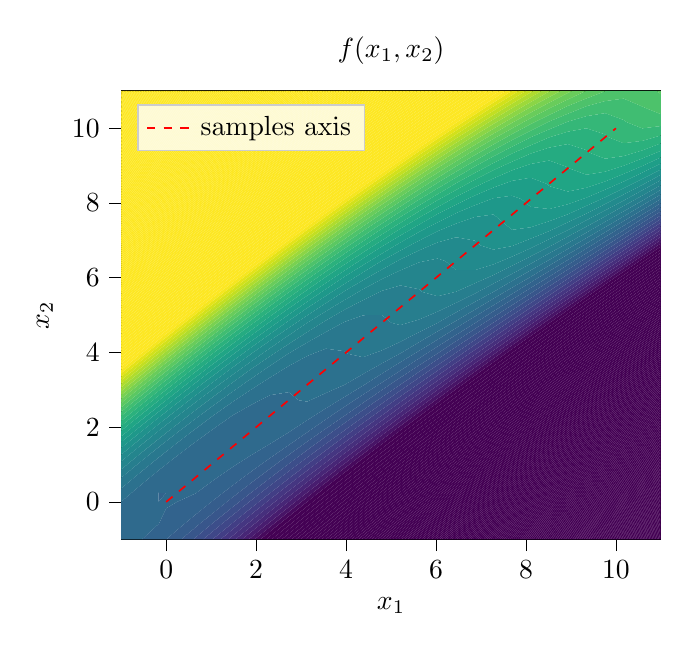
\begin{tikzpicture}

\definecolor{darkcyan30152138}{RGB}{30,152,138}
\definecolor{darkcyan30158136}{RGB}{30,158,136}
\definecolor{darkcyan32145140}{RGB}{32,145,140}
\definecolor{darkcyan34138141}{RGB}{34,138,141}
\definecolor{darkcyan36133141}{RGB}{36,133,141}
\definecolor{darkcyan39126142}{RGB}{39,126,142}
\definecolor{darkgray176}{RGB}{176,176,176}
\definecolor{darkslateblue5099141}{RGB}{50,99,141}
\definecolor{darkslateblue5393140}{RGB}{53,93,140}
\definecolor{darkslateblue5686139}{RGB}{56,86,139}
\definecolor{darkslateblue6078138}{RGB}{60,78,138}
\definecolor{darkslateblue6371136}{RGB}{63,71,136}
\definecolor{darkslateblue6662133}{RGB}{66,62,133}
\definecolor{darkslateblue6954129}{RGB}{69,54,129}
\definecolor{darkslateblue7047124}{RGB}{70,47,124}
\definecolor{darkslateblue7138118}{RGB}{71,38,118}
\definecolor{gold22822724}{RGB}{228,227,24}
\definecolor{gold24623031}{RGB}{246,230,31}
\definecolor{gold25323136}{RGB}{253,231,36}
\definecolor{greenyellow19422334}{RGB}{194,223,34}
\definecolor{greenyellow21022527}{RGB}{210,225,27}
\definecolor{indigo68184}{RGB}{68,1,84}
\definecolor{indigo70992}{RGB}{70,9,92}
\definecolor{indigo7120102}{RGB}{71,20,102}
\definecolor{indigo7229111}{RGB}{72,29,111}
\definecolor{lightgray204}{RGB}{204,204,204}
\definecolor{mediumseagreen10520491}{RGB}{105,204,91}
\definecolor{mediumseagreen32165133}{RGB}{32,165,133}
\definecolor{mediumseagreen37171129}{RGB}{37,171,129}
\definecolor{mediumseagreen43177125}{RGB}{43,177,125}
\definecolor{mediumseagreen53183120}{RGB}{53,183,120}
\definecolor{mediumseagreen64189114}{RGB}{64,189,114}
\definecolor{mediumseagreen77194107}{RGB}{77,194,107}
\definecolor{mediumseagreen9120098}{RGB}{91,200,98}
\definecolor{steelblue47106141}{RGB}{47,106,141}
\definecolor{teal41120142}{RGB}{41,120,142}
\definecolor{teal44113142}{RGB}{44,113,142}
\definecolor{yellowgreen12120981}{RGB}{121,209,81}
\definecolor{yellowgreen13921370}{RGB}{139,213,70}
\definecolor{yellowgreen15721758}{RGB}{157,217,58}
\definecolor{yellowgreen17522046}{RGB}{175,220,46}

\begin{axis}[
legend cell align={left},
legend style={
  fill opacity=0.8,
  draw opacity=1,
  text opacity=1,
  at={(0.03,0.97)},
  anchor=north west,
  draw=lightgray204
},
tick align=outside,
tick pos=left,
title={\(\displaystyle f(x_1, x_2)\)},
x grid style={darkgray176},
xlabel={\(\displaystyle x_1\)},
xmin=-1, xmax=11,
xtick style={color=black},
y grid style={darkgray176},
ylabel={\(\displaystyle x_2\)},
ymin=-1, ymax=11,
ytick style={color=black}
]
\addplot [draw=none, fill=indigo68184, forget plot]
table{%
x  y
11 -1
11 -0.997974577454952
10.997889066822 -1
11 -1
};
\addplot [draw=none, fill=indigo68184, forget plot]
table{%
x  y
11 -0.997974577454952
11 -0.965567816734181
10.9641141359732 -1
10.997889066822 -1
11 -0.997974577454952
};
\addplot [draw=none, fill=indigo68184, forget plot]
table{%
x  y
11 -0.965567816734181
11 -0.933161056013409
10.9303392051245 -1
10.9641141359732 -1
11 -0.965567816734181
};
\addplot [draw=none, fill=indigo68184, forget plot]
table{%
x  y
11 -0.933161056013409
11 -0.900754295292638
10.8965642742757 -1
10.9303392051245 -1
11 -0.933161056013409
};
\addplot [draw=none, fill=indigo68184, forget plot]
table{%
x  y
11 -0.900754295292638
11 -0.868347534571867
10.862789343427 -1
10.8965642742757 -1
11 -0.900754295292638
};
\addplot [draw=none, fill=indigo68184, forget plot]
table{%
x  y
11 -0.868347534571867
11 -0.835940773851096
10.8290144125782 -1
10.862789343427 -1
11 -0.868347534571867
};
\addplot [draw=none, fill=indigo68184, forget plot]
table{%
x  y
11 -0.835940773851096
11 -0.803534013130325
10.7952394817295 -1
10.8290144125782 -1
11 -0.835940773851096
};
\addplot [draw=none, fill=indigo68184, forget plot]
table{%
x  y
11 -0.803534013130325
11 -0.771127252409554
10.7614645508808 -1
10.7952394817295 -1
11 -0.803534013130325
};
\addplot [draw=none, fill=indigo68184, forget plot]
table{%
x  y
11 -0.771127252409554
11 -0.738720491688783
10.727689620032 -1
10.7614645508808 -1
11 -0.771127252409554
};
\addplot [draw=none, fill=indigo68184, forget plot]
table{%
x  y
11 -0.738720491688783
11 -0.706313730968011
10.6939146891833 -1
10.727689620032 -1
11 -0.738720491688783
};
\addplot [draw=none, fill=indigo68184, forget plot]
table{%
x  y
11 -0.706313730968011
11 -0.67390697024724
10.6601397583345 -1
10.6939146891833 -1
11 -0.706313730968011
};
\addplot [draw=none, fill=indigo68184, forget plot]
table{%
x  y
11 -0.67390697024724
11 -0.641500209526469
10.6263648274858 -1
10.6601397583345 -1
11 -0.67390697024724
};
\addplot [draw=none, fill=indigo68184, forget plot]
table{%
x  y
11 -0.641500209526469
11 -0.609093448805698
10.5925898966371 -1
10.6263648274858 -1
11 -0.641500209526469
};
\addplot [draw=none, fill=indigo68184, forget plot]
table{%
x  y
10.5862068965517 -1
10.5925898966371 -1
11 -0.609093448805698
11 -0.586206896551724
11 -0.576356459723599
10.9896999890564 -0.586206896551724
10.5862068965517 -0.972758770462749
10.5578232531042 -1
10.5862068965517 -1
};
\addplot [draw=none, fill=indigo68184, forget plot]
table{%
x  y
10.5862068965517 -0.972758770462749
10.9896999890564 -0.586206896551724
11 -0.576356459723599
11 -0.54282560266333
10.9546387830718 -0.586206896551724
10.5862068965517 -0.939169657968178
10.5228255158889 -1
10.5578232531042 -1
10.5862068965517 -0.972758770462749
};
\addplot [draw=none, fill=indigo68184, forget plot]
table{%
x  y
10.5862068965517 -0.939169657968178
10.9546387830718 -0.586206896551724
11 -0.54282560266333
11 -0.509294745603061
10.9195775770872 -0.586206896551724
10.5862068965517 -0.905580545473607
10.4878277786736 -1
10.5228255158889 -1
10.5862068965517 -0.939169657968178
};
\addplot [draw=none, fill=indigo68184, forget plot]
table{%
x  y
10.5862068965517 -0.905580545473607
10.9195775770872 -0.586206896551724
11 -0.509294745603061
11 -0.475763888542792
10.8845163711026 -0.586206896551724
10.5862068965517 -0.871991432979037
10.4528300414584 -1
10.4878277786736 -1
10.5862068965517 -0.905580545473607
};
\addplot [draw=none, fill=indigo68184, forget plot]
table{%
x  y
10.5862068965517 -0.871991432979037
10.8845163711026 -0.586206896551724
11 -0.475763888542792
11 -0.442233031482524
10.8494551651181 -0.586206896551724
10.5862068965517 -0.838402320484466
10.4178323042431 -1
10.4528300414584 -1
10.5862068965517 -0.871991432979037
};
\addplot [draw=none, fill=indigo68184, forget plot]
table{%
x  y
10.5862068965517 -0.838402320484466
10.8494551651181 -0.586206896551724
11 -0.442233031482524
11 -0.408702174422255
10.8143939591335 -0.586206896551724
10.5862068965517 -0.804813207989895
10.3828345670278 -1
10.4178323042431 -1
10.5862068965517 -0.838402320484466
};
\addplot [draw=none, fill=indigo68184, forget plot]
table{%
x  y
10.5862068965517 -0.804813207989895
10.8143939591335 -0.586206896551724
11 -0.408702174422255
11 -0.375171317361986
10.7793327531489 -0.586206896551724
10.5862068965517 -0.771224095495325
10.3478368298126 -1
10.3828345670278 -1
10.5862068965517 -0.804813207989895
};
\addplot [draw=none, fill=indigo68184, forget plot]
table{%
x  y
10.5862068965517 -0.771224095495325
10.7793327531489 -0.586206896551724
11 -0.375171317361986
11 -0.341640460301717
10.7442715471643 -0.586206896551724
10.5862068965517 -0.737634983000754
10.3128390925973 -1
10.3478368298126 -1
10.5862068965517 -0.771224095495325
};
\addplot [draw=none, fill=indigo68184, forget plot]
table{%
x  y
10.5862068965517 -0.737634983000754
10.7442715471643 -0.586206896551724
11 -0.341640460301717
11 -0.308109603241449
10.7092103411797 -0.586206896551724
10.5862068965517 -0.704045870506183
10.277841355382 -1
10.3128390925973 -1
10.5862068965517 -0.737634983000754
};
\addplot [draw=none, fill=indigo68184, forget plot]
table{%
x  y
10.5862068965517 -0.704045870506183
10.7092103411797 -0.586206896551724
11 -0.308109603241449
11 -0.27457874618118
10.6741491351951 -0.586206896551724
10.5862068965517 -0.670456758011613
10.2428436181668 -1
10.277841355382 -1
10.5862068965517 -0.704045870506183
};
\addplot [draw=none, fill=indigo68184, forget plot]
table{%
x  y
10.5862068965517 -0.670456758011613
10.6741491351951 -0.586206896551724
11 -0.27457874618118
11 -0.241047889120911
10.6390879292106 -0.586206896551724
10.5862068965517 -0.636867645517042
10.2078458809515 -1
10.2428436181668 -1
10.5862068965517 -0.670456758011613
};
\addplot [draw=none, fill=indigo68184, forget plot]
table{%
x  y
10.5862068965517 -0.636867645517042
10.6390879292106 -0.586206896551724
11 -0.241047889120911
11 -0.207517032060642
10.604026723226 -0.586206896551724
10.5862068965517 -0.603278533022471
10.1728481437362 -1
10.2078458809515 -1
10.5862068965517 -0.636867645517042
};
\addplot [draw=none, fill=indigo68184, forget plot]
table{%
x  y
10.1724137931034 -1
10.1728481437362 -1
10.5862068965517 -0.603278533022471
10.604026723226 -0.586206896551724
11 -0.207517032060642
11 -0.173986175000374
10.5862068965517 -0.569094821121013
10.5683166335916 -0.586206896551724
10.1724137931034 -0.965571646933858
10.1365520479704 -1
10.1724137931034 -1
};
\addplot [draw=none, fill=indigo68184, forget plot]
table{%
x  y
10.1724137931034 -0.965571646933858
10.5683166335916 -0.586206896551724
10.5862068965517 -0.569094821121013
11 -0.173986175000374
11 -0.172413793103448
11 -0.139306937338338
10.9652599073598 -0.172413793103448
10.5862068965517 -0.534296561034018
10.5319358902954 -0.586206896551724
10.1724137931034 -0.930710640172025
10.1002396360123 -1
10.1365520479704 -1
10.1724137931034 -0.965571646933858
};
\addplot [draw=none, fill=indigo68184, forget plot]
table{%
x  y
10.1724137931034 -0.930710640172025
10.5319358902954 -0.586206896551724
10.5862068965517 -0.534296561034018
10.9652599073598 -0.172413793103448
11 -0.139306937338338
11 -0.104571198455271
10.9288105750738 -0.172413793103448
10.5862068965517 -0.499498300947022
10.4955551469992 -0.586206896551724
10.1724137931034 -0.895849633410192
10.0639272240543 -1
10.1002396360123 -1
10.1724137931034 -0.930710640172025
};
\addplot [draw=none, fill=indigo68184, forget plot]
table{%
x  y
10.1724137931034 -0.895849633410192
10.4955551469992 -0.586206896551724
10.5862068965517 -0.499498300947022
10.9288105750738 -0.172413793103448
11 -0.104571198455271
11 -0.0698354595722051
10.8923612427879 -0.172413793103448
10.5862068965517 -0.464700040860026
10.459174403703 -0.586206896551724
10.1724137931034 -0.860988626648359
10.0276148120962 -1
10.0639272240543 -1
10.1724137931034 -0.895849633410192
};
\addplot [draw=none, fill=indigo68184, forget plot]
table{%
x  y
10.1724137931034 -0.860988626648359
10.459174403703 -0.586206896551724
10.5862068965517 -0.464700040860026
10.8923612427879 -0.172413793103448
11 -0.0698354595722051
11 -0.0350997206891388
10.8559119105019 -0.172413793103448
10.5862068965517 -0.429901780773031
10.4227936604067 -0.586206896551724
10.1724137931034 -0.826127619886525
9.99130240013817 -1
10.0276148120962 -1
10.1724137931034 -0.860988626648359
};
\addplot [draw=none, fill=indigo68184, forget plot]
table{%
x  y
10.1724137931034 -0.826127619886525
10.4227936604067 -0.586206896551724
10.5862068965517 -0.429901780773031
10.8559119105019 -0.172413793103448
11 -0.0350997206891388
11 -0.000363981806072472
10.819462578216 -0.172413793103448
10.5862068965517 -0.395103520686035
10.3864129171105 -0.586206896551724
10.1724137931034 -0.791266613124692
9.95498998818012 -1
9.99130240013817 -1
10.1724137931034 -0.826127619886525
};
\addplot [draw=none, fill=indigo68184, forget plot]
table{%
x  y
10.1724137931034 -0.791266613124692
10.3864129171105 -0.586206896551724
10.5862068965517 -0.395103520686035
10.819462578216 -0.172413793103448
11 -0.000363981806072472
11 0.0343717570769939
10.7830132459301 -0.172413793103448
10.5862068965517 -0.360305260599039
10.3500321738143 -0.586206896551724
10.1724137931034 -0.756405606362859
9.91867757622206 -1
9.95498998818012 -1
10.1724137931034 -0.791266613124692
};
\addplot [draw=none, fill=indigo68184, forget plot]
table{%
x  y
10.1724137931034 -0.756405606362859
10.3500321738143 -0.586206896551724
10.5862068965517 -0.360305260599039
10.7830132459301 -0.172413793103448
11 0.0343717570769939
11 0.0691074959600602
10.7465639136441 -0.172413793103448
10.5862068965517 -0.325507000512044
10.3136514305181 -0.586206896551724
10.1724137931034 -0.721544599601026
9.88236516426401 -1
9.91867757622206 -1
10.1724137931034 -0.756405606362859
};
\addplot [draw=none, fill=indigo68184, forget plot]
table{%
x  y
10.1724137931034 -0.721544599601026
10.3136514305181 -0.586206896551724
10.5862068965517 -0.325507000512044
10.7465639136441 -0.172413793103448
11 0.0691074959600602
11 0.103843234843127
10.7101145813582 -0.172413793103448
10.5862068965517 -0.290708740425048
10.2772706872219 -0.586206896551724
10.1724137931034 -0.686683592839193
9.84605275230596 -1
9.88236516426401 -1
10.1724137931034 -0.721544599601026
};
\addplot [draw=none, fill=indigo68184, forget plot]
table{%
x  y
10.1724137931034 -0.686683592839193
10.2772706872219 -0.586206896551724
10.5862068965517 -0.290708740425048
10.7101145813582 -0.172413793103448
11 0.103843234843127
11 0.138578973726193
10.6736652490722 -0.172413793103448
10.5862068965517 -0.255910480338052
10.2408899439256 -0.586206896551724
10.1724137931034 -0.65182258607736
9.80974034034791 -1
9.84605275230596 -1
10.1724137931034 -0.686683592839193
};
\addplot [draw=none, fill=indigo68184, forget plot]
table{%
x  y
10.1724137931034 -0.65182258607736
10.2408899439256 -0.586206896551724
10.5862068965517 -0.255910480338052
10.6736652490722 -0.172413793103448
11 0.138578973726193
11 0.173314712609259
10.6372159167863 -0.172413793103448
10.5862068965517 -0.221112220251057
10.2045092006294 -0.586206896551724
10.1724137931034 -0.616961579315527
9.77342792838985 -1
9.80974034034791 -1
10.1724137931034 -0.65182258607736
};
\addplot [draw=none, fill=indigo68184, forget plot]
table{%
x  y
9.75862068965517 -1
9.77342792838985 -1
10.1724137931034 -0.616961579315527
10.2045092006294 -0.586206896551724
10.5862068965517 -0.221112220251057
10.6372159167863 -0.172413793103448
11 0.173314712609259
11 0.208050451492326
10.6007665845004 -0.172413793103448
10.5862068965517 -0.186313960164061
10.1724137931034 -0.581946945467251
10.1679608704691 -0.586206896551724
9.75862068965517 -0.978541847302181
9.73627615367792 -1
9.75862068965517 -1
};
\addplot [draw=none, fill=indigo68184, forget plot]
table{%
x  y
9.75862068965517 -0.978541847302181
10.1679608704691 -0.586206896551724
10.1724137931034 -0.581946945467251
10.5862068965517 -0.186313960164061
10.6007665845004 -0.172413793103448
11 0.208050451492326
11 0.241379310344828
11 0.242838628829707
10.9984628575619 0.241379310344828
10.5862068965517 -0.150735313843001
10.5634595355384 -0.172413793103448
10.1724137931034 -0.545781707743167
10.1301573834233 -0.586206896551724
9.75862068965517 -0.942308831528325
9.6985464415296 -1
9.73627615367792 -1
9.75862068965517 -0.978541847302181
};
\addplot [draw=none, fill=indigo68184, forget plot]
table{%
x  y
9.75862068965517 -0.942308831528325
10.1301573834233 -0.586206896551724
10.1724137931034 -0.545781707743167
10.5634595355384 -0.172413793103448
10.5862068965517 -0.150735313843001
10.9984628575619 0.241379310344828
11 0.242838628829707
11 0.278869068338948
10.9605109517873 0.241379310344828
10.5862068965517 -0.114637601068767
10.5255819845179 -0.172413793103448
10.1724137931034 -0.509616470019083
10.0923538963775 -0.586206896551724
9.75862068965517 -0.906075815754469
9.66081672938128 -1
9.6985464415296 -1
9.75862068965517 -0.942308831528325
};
\addplot [draw=none, fill=indigo68184, forget plot]
table{%
x  y
9.75862068965517 -0.906075815754469
10.0923538963775 -0.586206896551724
10.1724137931034 -0.509616470019083
10.5255819845179 -0.172413793103448
10.5862068965517 -0.114637601068767
10.9605109517873 0.241379310344828
11 0.278869068338948
11 0.314899507848188
10.9225590460127 0.241379310344828
10.5862068965517 -0.0785398882945337
10.4877044334975 -0.172413793103448
10.1724137931034 -0.473451232294999
10.0545504093318 -0.586206896551724
9.75862068965517 -0.869842799980613
9.62308701723297 -1
9.66081672938128 -1
9.75862068965517 -0.906075815754469
};
\addplot [draw=none, fill=indigo68184, forget plot]
table{%
x  y
9.75862068965517 -0.869842799980613
10.0545504093318 -0.586206896551724
10.1724137931034 -0.473451232294999
10.4877044334975 -0.172413793103448
10.5862068965517 -0.0785398882945338
10.9225590460127 0.241379310344828
11 0.314899507848188
11 0.350929947357429
10.8846071402382 0.241379310344828
10.5862068965517 -0.0424421755203
10.4498268824771 -0.172413793103448
10.1724137931034 -0.437285994570915
10.016746922286 -0.586206896551724
9.75862068965517 -0.833609784206757
9.58535730508465 -1
9.62308701723297 -1
9.75862068965517 -0.869842799980613
};
\addplot [draw=none, fill=indigo68184, forget plot]
table{%
x  y
9.75862068965517 -0.833609784206757
10.016746922286 -0.586206896551724
10.1724137931034 -0.437285994570915
10.4498268824771 -0.172413793103448
10.5862068965517 -0.0424421755203
10.8846071402382 0.241379310344828
11 0.350929947357429
11 0.386960386866669
10.8466552344636 0.241379310344828
10.5862068965517 -0.00634446274606631
10.4119493314567 -0.172413793103448
10.1724137931034 -0.40112075684683
9.97894343524018 -0.586206896551724
9.75862068965517 -0.797376768432901
9.54762759293633 -1
9.58535730508465 -1
9.75862068965517 -0.833609784206757
};
\addplot [draw=none, fill=indigo68184, forget plot]
table{%
x  y
9.75862068965517 -0.797376768432901
9.97894343524018 -0.586206896551724
10.1724137931034 -0.40112075684683
10.4119493314567 -0.172413793103448
10.5862068965517 -0.00634446274606631
10.8466552344636 0.241379310344828
11 0.386960386866669
11 0.42299082637591
10.808703328689 0.241379310344828
10.5862068965517 0.0297532500281674
10.3740717804363 -0.172413793103448
10.1724137931034 -0.364955519122746
9.94113994819439 -0.586206896551724
9.75862068965517 -0.761143752659045
9.50989788078802 -1
9.54762759293633 -1
9.75862068965517 -0.797376768432901
};
\addplot [draw=none, fill=indigo68184, forget plot]
table{%
x  y
9.75862068965517 -0.761143752659045
9.94113994819439 -0.586206896551724
10.1724137931034 -0.364955519122746
10.3740717804363 -0.172413793103448
10.5862068965517 0.0297532500281674
10.808703328689 0.241379310344828
11 0.42299082637591
11 0.45902126588515
10.7707514229144 0.241379310344828
10.5862068965517 0.0658509628024011
10.3361942294159 -0.172413793103448
10.1724137931034 -0.328790281398662
9.9033364611486 -0.586206896551724
9.75862068965517 -0.724910736885189
9.4721681686397 -1
9.50989788078802 -1
9.75862068965517 -0.761143752659045
};
\addplot [draw=none, fill=indigo68184, forget plot]
table{%
x  y
9.75862068965517 -0.724910736885189
9.9033364611486 -0.586206896551724
10.1724137931034 -0.328790281398662
10.3361942294159 -0.172413793103448
10.5862068965517 0.0658509628024011
10.7707514229144 0.241379310344828
11 0.45902126588515
11 0.495051705394391
10.7327995171398 0.241379310344828
10.5862068965517 0.101948675576635
10.2983166783955 -0.172413793103448
10.1724137931034 -0.292625043674578
9.86553297410281 -0.586206896551724
9.75862068965517 -0.688677721111333
9.43443845649138 -1
9.4721681686397 -1
9.75862068965517 -0.724910736885189
};
\addplot [draw=none, fill=indigo68184, forget plot]
table{%
x  y
9.75862068965517 -0.688677721111333
9.86553297410281 -0.586206896551724
10.1724137931034 -0.292625043674578
10.2983166783955 -0.172413793103448
10.5862068965517 0.101948675576635
10.7327995171398 0.241379310344828
11 0.495051705394391
11 0.531082144903631
10.6948476113653 0.241379310344828
10.5862068965517 0.138046388350869
10.2604391273751 -0.172413793103448
10.1724137931034 -0.256459805950494
9.82772948705703 -0.586206896551724
9.75862068965517 -0.652444705337477
9.39670874434307 -1
9.43443845649138 -1
9.75862068965517 -0.688677721111333
};
\addplot [draw=none, fill=indigo68184, forget plot]
table{%
x  y
9.75862068965517 -0.652444705337477
9.82772948705703 -0.586206896551724
10.1724137931034 -0.256459805950494
10.2604391273751 -0.172413793103448
10.5862068965517 0.138046388350869
10.6948476113653 0.241379310344828
11 0.531082144903631
11 0.567112584412872
10.6568957055907 0.241379310344828
10.5862068965517 0.174144101125102
10.2225615763547 -0.172413793103448
10.1724137931034 -0.22029456822641
9.78992600001124 -0.586206896551724
9.75862068965517 -0.616211689563621
9.35897903219475 -1
9.39670874434307 -1
9.75862068965517 -0.652444705337477
};
\addplot [draw=none, fill=indigo68184, forget plot]
table{%
x  y
9.3448275862069 -1
9.35897903219475 -1
9.75862068965517 -0.616211689563621
9.78992600001124 -0.586206896551724
10.1724137931034 -0.22029456822641
10.2225615763547 -0.172413793103448
10.5862068965517 0.174144101125102
10.6568957055907 0.241379310344828
11 0.567112584412872
11 0.603143023922112
10.6189437998161 0.241379310344828
10.5862068965517 0.210241813899336
10.1846840253343 -0.172413793103448
10.1724137931034 -0.184129330502325
9.75862068965517 -0.579736133880164
9.75185804587955 -0.586206896551724
9.3448275862069 -0.976429400321786
9.32029166496461 -1
9.3448275862069 -1
};
\addplot [draw=none, fill=indigo68184, forget plot]
table{%
x  y
9.3448275862069 -0.976429400321786
9.75185804587955 -0.586206896551724
9.75862068965517 -0.579736133880164
10.1724137931035 -0.184129330502325
10.1846840253343 -0.172413793103448
10.5862068965517 0.210241813899336
10.6189437998161 0.241379310344828
11 0.603143023922112
11 0.639173463431353
10.5862068965517 0.24653193849172
10.5807787830927 0.241379310344828
10.1724137931034 -0.147013821024711
10.1457621656462 -0.172413793103448
9.75862068965517 -0.542092129336922
9.71251600755498 -0.586206896551724
9.3448275862069 -0.938711956003789
9.28102952247011 -1
9.32029166496461 -1
9.3448275862069 -0.976429400321786
};
\addplot [draw=none, fill=indigo68184, forget plot]
table{%
x  y
9.3448275862069 -0.938711956003789
9.71251600755498 -0.586206896551724
9.75862068965517 -0.542092129336922
10.1457621656462 -0.172413793103448
10.1724137931034 -0.147013821024711
10.5807787830927 0.241379310344828
10.5862068965517 0.24653193849172
11 0.639173463431353
11 0.655172413793103
11 0.675979440510427
10.9779930457907 0.655172413793103
10.5862068965517 0.284029918126438
10.5412759736257 0.241379310344828
10.1724137931034 -0.109442970822282
10.1063399056631 -0.172413793103448
9.75862068965517 -0.50444812479368
9.67317396923041 -0.586206896551724
9.3448275862069 -0.900994511685792
9.24176737997561 -1
9.28102952247011 -1
9.3448275862069 -0.938711956003789
};
\addplot [draw=none, fill=indigo68184, forget plot]
table{%
x  y
9.3448275862069 -0.900994511685792
9.67317396923041 -0.586206896551724
9.75862068965517 -0.50444812479368
10.1063399056631 -0.172413793103448
10.1724137931034 -0.109442970822282
10.5412759736257 0.241379310344828
10.5862068965517 0.284029918126438
10.9779930457907 0.655172413793103
11 0.675979440510427
11 0.713404831702555
10.9384093570004 0.655172413793103
10.5862068965517 0.321527897761156
10.5017731641586 0.241379310344828
10.1724137931034 -0.0718721206198523
10.0669176456801 -0.172413793103448
9.75862068965517 -0.466804120250438
9.63383193090584 -0.586206896551724
9.3448275862069 -0.863277067367795
9.20250523748111 -1
9.24176737997561 -1
9.3448275862069 -0.900994511685792
};
\addplot [draw=none, fill=indigo68184, forget plot]
table{%
x  y
9.3448275862069 -0.863277067367795
9.63383193090584 -0.586206896551724
9.75862068965517 -0.466804120250438
10.0669176456801 -0.172413793103448
10.1724137931034 -0.0718721206198523
10.5017731641586 0.241379310344828
10.5862068965517 0.321527897761156
10.9384093570004 0.655172413793103
11 0.713404831702555
11 0.750830222894682
10.8988256682101 0.655172413793103
10.5862068965517 0.359025877395874
10.4622703546915 0.241379310344828
10.1724137931034 -0.0343012704174231
10.0274953856971 -0.172413793103448
9.75862068965517 -0.429160115707196
9.59448989258127 -0.586206896551724
9.3448275862069 -0.825559623049798
9.16324309498661 -1
9.20250523748111 -1
9.3448275862069 -0.863277067367795
};
\addplot [draw=none, fill=indigo68184, forget plot]
table{%
x  y
9.3448275862069 -0.825559623049798
9.59448989258127 -0.586206896551724
9.75862068965517 -0.429160115707196
10.0274953856971 -0.172413793103448
10.1724137931034 -0.0343012704174231
10.4622703546915 0.241379310344828
10.5862068965517 0.359025877395874
10.8988256682101 0.655172413793103
11 0.750830222894682
11 0.78825561408681
10.8592419794198 0.655172413793103
10.5862068965517 0.396523857030592
10.4227675452245 0.241379310344828
10.1724137931034 0.00326957978500618
9.98807312571412 -0.172413793103448
9.75862068965517 -0.391516111163954
9.5551478542567 -0.586206896551724
9.3448275862069 -0.787842178731801
9.12398095249211 -1
9.16324309498661 -1
9.3448275862069 -0.825559623049798
};
\addplot [draw=none, fill=indigo68184, forget plot]
table{%
x  y
9.3448275862069 -0.787842178731801
9.5551478542567 -0.586206896551724
9.75862068965517 -0.391516111163954
9.98807312571412 -0.172413793103448
10.1724137931034 0.00326957978500617
10.4227675452245 0.241379310344828
10.5862068965517 0.396523857030592
10.8592419794198 0.655172413793103
11 0.78825561408681
11 0.825681005278938
10.8196582906295 0.655172413793103
10.5862068965517 0.43402183666531
10.3832647357574 0.241379310344828
10.1724137931034 0.0408404299874355
9.94865086573111 -0.172413793103448
9.75862068965517 -0.353872106620712
9.51580581593212 -0.586206896551724
9.3448275862069 -0.750124734413804
9.08471880999761 -1
9.12398095249211 -1
9.3448275862069 -0.787842178731801
};
\addplot [draw=none, fill=indigo68184, forget plot]
table{%
x  y
9.3448275862069 -0.750124734413804
9.51580581593212 -0.586206896551724
9.75862068965517 -0.353872106620712
9.94865086573111 -0.172413793103448
10.1724137931034 0.0408404299874355
10.3832647357574 0.241379310344828
10.5862068965517 0.43402183666531
10.8196582906295 0.655172413793103
11 0.825681005278938
11 0.863106396471066
10.7800746018392 0.655172413793103
10.5862068965517 0.471519816300028
10.3437619262904 0.241379310344828
10.1724137931034 0.0784112801898647
9.9092286057481 -0.172413793103448
9.75862068965517 -0.31622810207747
9.47646377760755 -0.586206896551724
9.3448275862069 -0.712407290095807
9.04545666750311 -1
9.08471880999761 -1
9.3448275862069 -0.750124734413804
};
\addplot [draw=none, fill=indigo68184, forget plot]
table{%
x  y
9.3448275862069 -0.712407290095807
9.47646377760755 -0.586206896551724
9.75862068965517 -0.31622810207747
9.9092286057481 -0.172413793103448
10.1724137931034 0.0784112801898647
10.3437619262904 0.241379310344828
10.5862068965517 0.471519816300028
10.7800746018392 0.655172413793103
11 0.863106396471066
11 0.900531787663194
10.7404909130489 0.655172413793103
10.5862068965517 0.509017795934746
10.3042591168233 0.241379310344828
10.1724137931034 0.115982130392294
9.8698063457651 -0.172413793103448
9.75862068965517 -0.278584097534228
9.43712173928298 -0.586206896551724
9.3448275862069 -0.67468984577781
9.00619452500861 -1
9.04545666750311 -1
9.3448275862069 -0.712407290095807
};
\addplot [draw=none, fill=indigo68184, forget plot]
table{%
x  y
9.3448275862069 -0.67468984577781
9.43712173928298 -0.586206896551724
9.75862068965517 -0.278584097534228
9.8698063457651 -0.172413793103448
10.1724137931034 0.115982130392294
10.3042591168233 0.241379310344828
10.5862068965517 0.509017795934746
10.7404909130489 0.655172413793103
11 0.900531787663194
11 0.937957178855322
10.7009072242585 0.655172413793103
10.5862068965517 0.546515775569464
10.2647563073563 0.241379310344828
10.1724137931034 0.153552980594723
9.83038408578209 -0.172413793103448
9.75862068965517 -0.240940092990986
9.39777970095841 -0.586206896551724
9.3448275862069 -0.636972401459813
8.96693238251411 -1
9.00619452500861 -1
9.3448275862069 -0.67468984577781
};
\addplot [draw=none, fill=indigo68184, forget plot]
table{%
x  y
8.93103448275862 -1
8.96693238251411 -1
9.3448275862069 -0.636972401459813
9.39777970095841 -0.586206896551724
9.75862068965517 -0.240940092990986
9.83038408578209 -0.172413793103448
10.1724137931034 0.153552980594723
10.2647563073563 0.241379310344828
10.5862068965517 0.546515775569464
10.7009072242585 0.655172413793103
11 0.937957178855322
11 0.97538257004745
10.6613235354682 0.655172413793103
10.5862068965517 0.584013755204182
10.2252534978892 0.241379310344828
10.1724137931034 0.191123830797153
9.79096182579908 -0.172413793103448
9.75862068965517 -0.203296088447744
9.35843766263383 -0.586206896551724
9.3448275862069 -0.599254957141816
8.93103448275862 -0.996630054188027
8.92752781309116 -1
8.93103448275862 -1
};
\addplot [draw=none, fill=indigo68184, forget plot]
table{%
x  y
8.93103448275862 -0.996630054188027
9.3448275862069 -0.599254957141816
9.35843766263383 -0.586206896551724
9.75862068965517 -0.203296088447744
9.79096182579908 -0.172413793103448
10.1724137931034 0.191123830797153
10.2252534978892 0.241379310344828
10.5862068965517 0.584013755204182
10.6613235354682 0.655172413793103
11 0.97538257004745
11 1.01280796123958
10.6217398466779 0.655172413793103
10.5862068965517 0.6215117348389
10.1857506884222 0.241379310344828
10.1724137931034 0.228694680999582
9.75862068965517 -0.165378099402097
9.75123850829235 -0.172413793103448
9.3448275862069 -0.560535879919962
9.31800393775182 -0.586206896551724
8.93103448275862 -0.957301354408403
8.88660348781333 -1
8.92752781309116 -1
8.93103448275862 -0.996630054188027
};
\addplot [draw=none, fill=indigo68184, forget plot]
table{%
x  y
8.93103448275862 -0.957301354408403
9.31800393775182 -0.586206896551724
9.3448275862069 -0.560535879919962
9.75123850829235 -0.172413793103448
9.75862068965517 -0.165378099402097
10.1724137931034 0.228694680999582
10.1857506884222 0.241379310344828
10.5862068965517 0.6215117348389
10.6217398466779 0.655172413793103
11 1.01280796123958
11 1.05023335243171
10.5862068965517 0.659164574430458
10.5819832033814 0.655172413793103
10.1724137931035 0.267271882171804
10.1451330521496 0.241379310344828
9.75862068965517 -0.12620875954054
9.71014019119758 -0.172413793103448
9.3448275862069 -0.52128702185872
9.27699280110696 -0.586206896551724
8.93103448275862 -0.91797265462878
8.84567916253551 -1
8.88660348781333 -1
8.93103448275862 -0.957301354408403
};
\addplot [draw=none, fill=indigo68184, forget plot]
table{%
x  y
8.93103448275862 -0.91797265462878
9.27699280110696 -0.586206896551724
9.3448275862069 -0.52128702185872
9.71014019119758 -0.172413793103448
9.75862068965517 -0.12620875954054
10.1451330521496 0.241379310344828
10.1724137931034 0.267271882171804
10.5819832033814 0.655172413793103
10.5862068965517 0.659164574430458
11 1.05023335243171
11 1.06896551724138
11 1.08841161731603
10.9793404688278 1.06896551724138
10.5862068965517 0.698175840615089
10.540709408683 0.655172413793104
10.1724137931034 0.306362025390001
10.1039471831633 0.241379310344828
9.75862068965517 -0.0870394196789835
9.66904187410281 -0.172413793103448
9.3448275862069 -0.482038163797479
9.23598166446209 -0.586206896551724
8.93103448275862 -0.878643954849156
8.80475483725768 -1
8.84567916253551 -1
8.93103448275862 -0.91797265462878
};
\addplot [draw=none, fill=indigo68184, forget plot]
table{%
x  y
8.93103448275862 -0.878643954849156
9.23598166446209 -0.586206896551724
9.3448275862069 -0.482038163797479
9.66904187410281 -0.172413793103448
9.75862068965517 -0.0870394196789835
10.1039471831633 0.241379310344828
10.1724137931034 0.306362025390001
10.540709408683 0.655172413793103
10.5862068965517 0.698175840615089
10.9793404688278 1.06896551724138
11 1.08841161731603
11 1.12734432414603
10.9379783721974 1.06896551724138
10.5862068965517 0.73718710679972
10.4994356139845 0.655172413793103
10.1724137931034 0.345452168608199
10.0627613141769 0.241379310344828
9.75862068965517 -0.0478700798174268
9.62794355700803 -0.172413793103448
9.3448275862069 -0.442789305736237
9.19497052781723 -0.586206896551724
8.93103448275862 -0.839315255069532
8.76383051197985 -1
8.80475483725768 -1
8.93103448275862 -0.878643954849156
};
\addplot [draw=none, fill=indigo68184, forget plot]
table{%
x  y
8.93103448275862 -0.839315255069532
9.19497052781723 -0.586206896551724
9.3448275862069 -0.442789305736237
9.62794355700803 -0.172413793103448
9.75862068965517 -0.0478700798174268
10.0627613141769 0.241379310344828
10.1724137931034 0.345452168608198
10.4994356139845 0.655172413793103
10.5862068965517 0.73718710679972
10.9379783721974 1.06896551724138
11 1.12734432414603
11 1.16627703097604
10.896616275567 1.06896551724138
10.5862068965517 0.77619837298435
10.4581618192861 0.655172413793103
10.1724137931034 0.384542311826396
10.0215754451906 0.241379310344828
9.75862068965517 -0.00870073995587016
9.58684523991326 -0.172413793103448
9.3448275862069 -0.403540447674995
9.15395939117236 -0.586206896551724
8.93103448275862 -0.799986555289909
8.72290618670203 -1
8.76383051197985 -1
8.93103448275862 -0.839315255069532
};
\addplot [draw=none, fill=indigo68184, forget plot]
table{%
x  y
8.93103448275862 -0.799986555289909
9.15395939117236 -0.586206896551724
9.3448275862069 -0.403540447674995
9.58684523991326 -0.172413793103448
9.75862068965517 -0.00870073995587017
10.0215754451906 0.241379310344828
10.1724137931034 0.384542311826396
10.4581618192861 0.655172413793103
10.5862068965517 0.77619837298435
10.896616275567 1.06896551724138
11 1.16627703097604
11 1.20520973780604
10.8552541789366 1.06896551724138
10.5862068965517 0.815209639168981
10.4168880245876 0.655172413793103
10.1724137931034 0.423632455044593
9.98038957620426 0.241379310344828
9.75862068965517 0.0304685999056865
9.54574692281848 -0.172413793103448
9.3448275862069 -0.364291589613753
9.1129482545275 -0.586206896551724
8.93103448275862 -0.760657855510285
8.6819818614242 -1
8.72290618670203 -1
8.93103448275862 -0.799986555289909
};
\addplot [draw=none, fill=indigo68184, forget plot]
table{%
x  y
8.93103448275862 -0.760657855510285
9.1129482545275 -0.586206896551724
9.3448275862069 -0.364291589613753
9.54574692281848 -0.172413793103448
9.75862068965517 0.0304685999056865
9.98038957620426 0.241379310344828
10.1724137931034 0.423632455044593
10.4168880245876 0.655172413793103
10.5862068965517 0.815209639168981
10.8552541789366 1.06896551724138
11 1.20520973780604
11 1.24414244463605
10.8138920823061 1.06896551724138
10.5862068965517 0.854220905353612
10.3756142298891 0.655172413793103
10.1724137931034 0.46272259826279
9.93920370721793 0.241379310344828
9.75862068965517 0.0696379397672432
9.50464860572371 -0.172413793103448
9.3448275862069 -0.325042731552511
9.07193711788264 -0.586206896551724
8.93103448275862 -0.721329155730661
8.64105753614637 -1
8.6819818614242 -1
8.93103448275862 -0.760657855510285
};
\addplot [draw=none, fill=indigo68184, forget plot]
table{%
x  y
8.93103448275862 -0.721329155730661
9.07193711788264 -0.586206896551724
9.3448275862069 -0.325042731552511
9.50464860572371 -0.172413793103448
9.75862068965517 0.0696379397672432
9.93920370721793 0.241379310344828
10.1724137931034 0.46272259826279
10.3756142298891 0.655172413793103
10.5862068965517 0.854220905353612
10.8138920823061 1.06896551724138
11 1.24414244463605
11 1.28307515146605
10.7725299856757 1.06896551724138
10.5862068965517 0.893232171538243
10.3343404351907 0.655172413793103
10.1724137931034 0.501812741480987
9.8980178382316 0.241379310344828
9.75862068965517 0.1088072796288
9.46355028862894 -0.172413793103448
9.3448275862069 -0.28579387349127
9.03092598123777 -0.586206896551724
8.93103448275862 -0.682000455951038
8.60013321086855 -1
8.64105753614637 -1
8.93103448275862 -0.721329155730661
};
\addplot [draw=none, fill=indigo68184, forget plot]
table{%
x  y
8.93103448275862 -0.682000455951038
9.03092598123777 -0.586206896551724
9.3448275862069 -0.28579387349127
9.46355028862894 -0.172413793103448
9.75862068965517 0.1088072796288
9.8980178382316 0.241379310344828
10.1724137931034 0.501812741480987
10.3343404351907 0.655172413793103
10.5862068965517 0.893232171538243
10.7725299856757 1.06896551724138
11 1.28307515146605
11 1.32200785829606
10.7311678890453 1.06896551724138
10.5862068965517 0.932243437722874
10.2930666404922 0.655172413793103
10.1724137931034 0.540902884699184
9.85683196924527 0.241379310344828
9.75862068965517 0.147976619490357
9.42245197153416 -0.172413793103448
9.3448275862069 -0.246545015430028
8.98991484459291 -0.586206896551724
8.93103448275862 -0.642671756171414
8.55920888559072 -1
8.60013321086855 -1
8.93103448275862 -0.682000455951038
};
\addplot [draw=none, fill=indigo68184, forget plot]
table{%
x  y
8.93103448275862 -0.642671756171414
8.9899148445929 -0.586206896551724
9.3448275862069 -0.246545015430028
9.42245197153416 -0.172413793103448
9.75862068965517 0.147976619490356
9.85683196924527 0.241379310344828
10.1724137931034 0.540902884699184
10.2930666404922 0.655172413793103
10.5862068965517 0.932243437722874
10.7311678890453 1.06896551724138
11 1.32200785829606
11 1.36094056512606
10.6898057924149 1.06896551724138
10.5862068965517 0.971254703907505
10.2517928457938 0.655172413793103
10.1724137931034 0.579993027917381
9.81564610025894 0.241379310344828
9.75862068965517 0.187145959351913
9.38135365443939 -0.172413793103448
9.3448275862069 -0.207296157368786
8.94890370794804 -0.586206896551724
8.93103448275862 -0.60334305639179
8.51828456031289 -1
8.55920888559072 -1
8.93103448275862 -0.642671756171414
};
\addplot [draw=none, fill=indigo68184, forget plot]
table{%
x  y
8.51724137931035 -1
8.51828456031289 -1
8.93103448275862 -0.60334305639179
8.94890370794804 -0.586206896551724
9.3448275862069 -0.207296157368786
9.38135365443939 -0.172413793103448
9.75862068965517 0.187145959351913
9.81564610025894 0.241379310344828
10.1724137931034 0.579993027917381
10.2517928457938 0.655172413793103
10.5862068965517 0.971254703907505
10.6898057924149 1.06896551724138
11 1.36094056512606
11 1.39987327195607
10.6484436957845 1.06896551724138
10.5862068965517 1.01026597009214
10.2105190510953 0.655172413793103
10.1724137931034 0.619083171135578
9.77446023127261 0.241379310344828
9.75862068965517 0.22631529921347
9.3448275862069 -0.167862506764604
9.3400523142684 -0.172413793103448
8.93103448275862 -0.563073163895168
8.90686726970648 -0.586206896551724
8.51724137931035 -0.959963483815025
8.47559720784294 -1
8.51724137931035 -1
};
\addplot [draw=none, fill=indigo68184, forget plot]
table{%
x  y
8.51724137931035 -0.959963483815025
8.90686726970648 -0.586206896551724
8.93103448275862 -0.563073163895168
9.3400523142684 -0.172413793103448
9.3448275862069 -0.167862506764604
9.75862068965517 0.22631529921347
9.77446023127261 0.241379310344828
10.1724137931034 0.619083171135578
10.2105190510953 0.655172413793103
10.5862068965517 1.01026597009214
10.6484436957845 1.06896551724138
11 1.39987327195607
11 1.43880597878607
10.6070815991541 1.06896551724138
10.5862068965517 1.04927723627677
10.1724137931035 0.658299778995489
10.1691039353024 0.655172413793103
9.75862068965517 0.266502636417143
9.73214639667001 0.241379310344828
9.3448275862069 -0.126952614329407
9.29712909502695 -0.172413793103448
8.93103448275862 -0.522076521378823
8.86403913605317 -0.586206896551724
8.51724137931035 -0.918879722525845
8.43286373943255 -1
8.47559720784294 -1
8.51724137931035 -0.959963483815025
};
\addplot [draw=none, fill=indigo68184, forget plot]
table{%
x  y
8.51724137931035 -0.918879722525845
8.86403913605317 -0.586206896551724
8.93103448275862 -0.522076521378823
9.29712909502695 -0.172413793103448
9.3448275862069 -0.126952614329407
9.73214639667001 0.241379310344828
9.75862068965517 0.266502636417143
10.1691039353024 0.655172413793103
10.1724137931034 0.658299778995489
10.5862068965517 1.04927723627677
10.6070815991541 1.06896551724138
11 1.43880597878607
11 1.47773868561608
10.5862068965517 1.08910110390748
10.5648036942602 1.06896551724138
10.1724137931034 0.69903726802095
10.1259892726003 0.655172413793103
9.75862068965517 0.307326145127331
9.6891276686893 0.241379310344828
9.3448275862069 -0.0860427218942103
9.25420587578551 -0.172413793103448
8.93103448275862 -0.481079878862477
8.82121100239985 -0.586206896551724
8.51724137931035 -0.877795961236665
8.39013027102216 -1
8.43286373943255 -1
8.51724137931035 -0.918879722525845
};
\addplot [draw=none, fill=indigo68184, forget plot]
table{%
x  y
8.51724137931035 -0.877795961236665
8.82121100239985 -0.586206896551724
8.93103448275862 -0.481079878862477
9.25420587578551 -0.172413793103448
9.3448275862069 -0.0860427218942102
9.6891276686893 0.241379310344828
9.75862068965517 0.307326145127331
10.1259892726003 0.655172413793103
10.1724137931034 0.69903726802095
10.5648036942602 1.06896551724138
10.5862068965517 1.08910110390748
11 1.47773868561608
11 1.48275862068966
11 1.51809455475095
10.9622762354123 1.48275862068966
10.5862068965517 1.12975293499212
10.5215926679983 1.06896551724138
10.1724137931034 0.739774757046411
10.0828746098982 0.655172413793103
9.75862068965517 0.34814965383752
9.64610894070858 0.241379310344828
9.3448275862069 -0.0451328294590136
9.21128265654407 -0.172413793103448
8.93103448275862 -0.440083236346131
8.77838286874654 -0.586206896551724
8.51724137931035 -0.836712199947485
8.34739680261177 -1
8.39013027102216 -1
8.51724137931035 -0.877795961236665
};
\addplot [draw=none, fill=indigo68184, forget plot]
table{%
x  y
8.51724137931035 -0.836712199947485
8.77838286874654 -0.586206896551724
8.93103448275862 -0.440083236346131
9.21128265654407 -0.172413793103448
9.3448275862069 -0.0451328294590136
9.64610894070858 0.241379310344828
9.75862068965517 0.348149653837519
10.0828746098982 0.655172413793103
10.1724137931034 0.739774757046411
10.5215926679983 1.06896551724138
10.5862068965517 1.12975293499212
10.9622762354123 1.48275862068966
11 1.51809455475095
11 1.55866108736155
10.9189684138703 1.48275862068966
10.5862068965517 1.17040476607675
10.4783816417364 1.06896551724138
10.1724137931034 0.780512246071872
10.0397599471961 0.655172413793103
9.75862068965517 0.388973162547708
9.60309021272786 0.241379310344828
9.3448275862069 -0.00422293702381701
9.16835943730262 -0.172413793103448
8.93103448275862 -0.399086593829786
8.73555473509322 -0.586206896551724
8.51724137931035 -0.795628438658305
8.30466333420138 -1
8.34739680261177 -1
8.51724137931035 -0.836712199947485
};
\addplot [draw=none, fill=indigo68184, forget plot]
table{%
x  y
8.51724137931035 -0.795628438658305
8.73555473509322 -0.586206896551724
8.93103448275862 -0.399086593829786
9.16835943730262 -0.172413793103448
9.3448275862069 -0.00422293702381697
9.60309021272787 0.241379310344828
9.75862068965517 0.388973162547708
10.0397599471961 0.655172413793103
10.1724137931034 0.780512246071872
10.4783816417364 1.06896551724138
10.5862068965517 1.17040476607675
10.9189684138703 1.48275862068966
11 1.55866108736155
11 1.59922761997214
10.8756605923284 1.48275862068966
10.5862068965517 1.21105659716138
10.4351706154745 1.06896551724138
10.1724137931034 0.821249735097333
9.99664528449397 0.655172413793103
9.75862068965517 0.429796671257896
9.56007148474715 0.241379310344828
9.3448275862069 0.0366869554113797
9.12543621806118 -0.172413793103448
8.93103448275862 -0.35808995131344
8.69272660143991 -0.586206896551724
8.51724137931035 -0.754544677369124
8.26192986579099 -1
8.30466333420138 -1
8.51724137931035 -0.795628438658305
};
\addplot [draw=none, fill=indigo68184, forget plot]
table{%
x  y
8.51724137931035 -0.754544677369124
8.69272660143991 -0.586206896551724
8.93103448275862 -0.35808995131344
9.12543621806118 -0.172413793103448
9.3448275862069 0.0366869554113796
9.56007148474715 0.241379310344828
9.75862068965517 0.429796671257896
9.99664528449397 0.655172413793103
10.1724137931034 0.821249735097333
10.4351706154745 1.06896551724138
10.5862068965517 1.21105659716138
10.8756605923284 1.48275862068966
11 1.59922761997214
11 1.63979415258274
10.8323527707865 1.48275862068966
10.5862068965517 1.25170842824601
10.3919595892127 1.06896551724138
10.1724137931034 0.861987224122794
9.95353062179187 0.655172413793103
9.75862068965517 0.470620179968084
9.51705275676643 0.241379310344828
9.3448275862069 0.0775968478465763
9.08251299881974 -0.172413793103448
8.93103448275862 -0.317093308797094
8.6498984677866 -0.586206896551724
8.51724137931035 -0.713460916079944
8.21919639738061 -1
8.26192986579099 -1
8.51724137931035 -0.754544677369124
};
\addplot [draw=none, fill=indigo68184, forget plot]
table{%
x  y
8.51724137931035 -0.713460916079944
8.6498984677866 -0.586206896551724
8.93103448275862 -0.317093308797094
9.08251299881974 -0.172413793103448
9.3448275862069 0.0775968478465763
9.51705275676643 0.241379310344828
9.75862068965517 0.470620179968084
9.95353062179187 0.655172413793103
10.1724137931034 0.861987224122794
10.3919595892127 1.06896551724138
10.5862068965517 1.25170842824601
10.8323527707865 1.48275862068966
11 1.63979415258274
11 1.68036068519334
10.7890449492446 1.48275862068966
10.5862068965517 1.29236025933065
10.3487485629508 1.06896551724138
10.1724137931034 0.902724713148255
9.91041595908977 0.655172413793103
9.75862068965517 0.511443688678273
9.47403402878572 0.241379310344828
9.3448275862069 0.118506740281773
9.0395897795783 -0.172413793103448
8.93103448275862 -0.276096666280749
8.60707033413328 -0.586206896551724
8.51724137931035 -0.672377154790764
8.17646292897022 -1
8.21919639738061 -1
8.51724137931035 -0.713460916079944
};
\addplot [draw=none, fill=indigo68184, forget plot]
table{%
x  y
8.51724137931035 -0.672377154790764
8.60707033413328 -0.586206896551724
8.93103448275862 -0.276096666280749
9.0395897795783 -0.172413793103448
9.3448275862069 0.118506740281773
9.47403402878572 0.241379310344828
9.75862068965517 0.511443688678273
9.91041595908977 0.655172413793103
10.1724137931034 0.902724713148255
10.3487485629508 1.06896551724138
10.5862068965517 1.29236025933065
10.7890449492446 1.48275862068966
11 1.68036068519334
11 1.72092721780393
10.7457371277027 1.48275862068966
10.5862068965517 1.33301209041528
10.3055375366889 1.06896551724138
10.1724137931034 0.943462202173716
9.86730129638767 0.655172413793103
9.75862068965517 0.552267197388461
9.431015300805 0.241379310344828
9.3448275862069 0.15941663271697
8.99666656033685 -0.172413793103448
8.93103448275862 -0.235100023764403
8.56424220047997 -0.586206896551724
8.51724137931035 -0.631293393501584
8.13372946055983 -1
8.17646292897022 -1
8.51724137931035 -0.672377154790764
};
\addplot [draw=none, fill=indigo68184, forget plot]
table{%
x  y
8.10344827586207 -1
8.13372946055983 -1
8.51724137931035 -0.631293393501584
8.56424220047997 -0.586206896551724
8.93103448275862 -0.235100023764403
8.99666656033685 -0.172413793103448
9.3448275862069 0.15941663271697
9.431015300805 0.241379310344828
9.75862068965517 0.552267197388461
9.86730129638767 0.655172413793103
10.1724137931034 0.943462202173716
10.3055375366889 1.06896551724138
10.5862068965517 1.33301209041528
10.7457371277027 1.48275862068966
11 1.72092721780393
11 1.76149375041453
10.7024293061608 1.48275862068966
10.5862068965517 1.37366392149991
10.262326510427 1.06896551724138
10.1724137931034 0.984199691199177
9.82418663368557 0.655172413793103
9.75862068965517 0.593090706098649
9.38799657282429 0.241379310344828
9.3448275862069 0.200326525152166
8.95374334109541 -0.172413793103448
8.93103448275862 -0.194103381248057
8.52141406682666 -0.586206896551724
8.51724137931035 -0.590209632212404
8.10344827586207 -0.987469240356652
8.09042005302995 -1
8.10344827586207 -1
};
\addplot [draw=none, fill=indigo68184, forget plot]
table{%
x  y
8.10344827586207 -0.987469240356652
8.51724137931035 -0.590209632212404
8.52141406682666 -0.586206896551724
8.93103448275862 -0.194103381248057
8.95374334109541 -0.172413793103448
9.3448275862069 0.200326525152166
9.38799657282429 0.241379310344828
9.75862068965517 0.593090706098649
9.82418663368557 0.655172413793103
10.1724137931034 0.984199691199177
10.262326510427 1.06896551724138
10.5862068965517 1.37366392149991
10.7024293061608 1.48275862068966
11 1.76149375041453
11 1.80206028302513
10.6591214846189 1.48275862068966
10.5862068965517 1.41431575258455
10.2191154841652 1.06896551724138
10.1724137931034 1.02493718022464
9.78107197098347 0.655172413793103
9.75862068965517 0.633914214808837
9.34497784484357 0.241379310344828
9.3448275862069 0.241236417587363
8.93103448275862 -0.15225165605055
8.9098808291885 -0.172413793103448
8.51724137931035 -0.547479958929357
8.47679390940033 -0.586206896551724
8.10344827586207 -0.944466460004474
8.04571008964587 -1
8.09042005302995 -1
8.10344827586207 -0.987469240356652
};
\addplot [draw=none, fill=indigo68184, forget plot]
table{%
x  y
8.10344827586207 -0.944466460004474
8.47679390940033 -0.586206896551724
8.51724137931035 -0.547479958929357
8.9098808291885 -0.172413793103448
8.93103448275862 -0.15225165605055
9.3448275862069 0.241236417587363
9.34497784484357 0.241379310344828
9.75862068965517 0.633914214808837
9.78107197098347 0.655172413793103
10.1724137931034 1.02493718022464
10.2191154841652 1.06896551724138
10.5862068965517 1.41431575258455
10.6591214846189 1.48275862068966
11 1.80206028302513
11 1.84262681563572
10.615813663077 1.48275862068966
10.5862068965517 1.45496758366918
10.1759044579033 1.06896551724138
10.1724137931034 1.0656746692501
9.75862068965517 0.675600423194613
9.73699266880856 0.655172413793103
9.3448275862069 0.283947834589427
9.29996252601431 0.241379310344828
8.93103448275862 -0.109439329052949
8.86496311379644 -0.172413793103448
8.51724137931035 -0.504572616595345
8.4319803107911 -0.586206896551724
8.10344827586207 -0.901463679652296
8.00100012626179 -1
8.04571008964587 -1
8.10344827586207 -0.944466460004474
};
\addplot [draw=none, fill=indigo68184, forget plot]
table{%
x  y
8.10344827586207 -0.901463679652296
8.4319803107911 -0.586206896551724
8.51724137931035 -0.504572616595345
8.86496311379644 -0.172413793103448
8.93103448275862 -0.109439329052949
9.29996252601431 0.241379310344828
9.3448275862069 0.283947834589427
9.73699266880856 0.655172413793103
9.75862068965517 0.675600423194613
10.1724137931034 1.0656746692501
10.1759044579033 1.06896551724138
10.5862068965517 1.45496758366918
10.615813663077 1.48275862068966
11 1.84262681563572
11 1.88319334824632
10.5862068965517 1.49618400055506
10.5718632280498 1.48275862068966
10.1724137931034 1.10805967318815
10.1308348068118 1.06896551724138
9.75862068965517 0.718223976382193
9.69186526168933 0.655172413793103
9.3448275862069 0.326665566130579
9.25494020891747 0.241379310344828
8.93103448275862 -0.0666270020553477
8.82004539840438 -0.172413793103448
8.51724137931035 -0.461665274261334
8.38716671218187 -0.586206896551724
8.10344827586207 -0.858460899300118
7.95629016287771 -1
8.00100012626179 -1
8.10344827586207 -0.901463679652296
};
\addplot [draw=none, fill=indigo68184, forget plot]
table{%
x  y
8.10344827586207 -0.858460899300118
8.38716671218187 -0.586206896551724
8.51724137931035 -0.461665274261334
8.82004539840438 -0.172413793103448
8.93103448275862 -0.0666270020553477
9.25494020891747 0.241379310344828
9.3448275862069 0.326665566130579
9.69186526168933 0.655172413793103
9.75862068965517 0.718223976382193
10.1308348068118 1.06896551724138
10.1724137931034 1.10805967318815
10.5718632280498 1.48275862068966
10.5862068965517 1.49618400055506
11 1.88319334824632
11 1.89655172413793
11 1.92495169644599
10.9695194028843 1.89655172413793
10.5862068965517 1.53862043735769
10.5265241621909 1.48275862068966
10.1724137931034 1.15058946237239
10.0856018179251 1.06896551724138
9.75862068965517 0.760847529569774
9.64673785457009 0.655172413793103
9.3448275862069 0.369383297671732
9.20991789182063 0.241379310344828
8.93103448275862 -0.0238146750577466
8.77512768301232 -0.172413793103448
8.51724137931035 -0.418757931927323
8.34235311357263 -0.586206896551724
8.10344827586207 -0.81545811894794
7.91158019949362 -1
7.95629016287771 -1
8.10344827586207 -0.858460899300118
};
\addplot [draw=none, fill=indigo68184, forget plot]
table{%
x  y
8.10344827586207 -0.81545811894794
8.34235311357263 -0.586206896551724
8.51724137931035 -0.418757931927323
8.77512768301232 -0.172413793103448
8.93103448275862 -0.0238146750577466
9.20991789182063 0.241379310344828
9.3448275862069 0.369383297671732
9.64673785457009 0.655172413793103
9.75862068965517 0.760847529569774
10.0856018179251 1.06896551724138
10.1724137931034 1.15058946237239
10.5265241621909 1.48275862068966
10.5862068965517 1.53862043735769
10.9695194028843 1.89655172413793
11 1.92495169644599
11 1.96729518978419
10.9240737613563 1.89655172413793
10.5862068965517 1.58105687416032
10.481185096332 1.48275862068966
10.1724137931034 1.19311925155662
10.0403688290384 1.06896551724138
9.75862068965517 0.803471082757354
9.60161044745085 0.655172413793103
9.3448275862069 0.412101029212884
9.1648955747238 0.241379310344828
8.93103448275862 0.0189976519398543
8.73020996762026 -0.172413793103448
8.51724137931035 -0.375850589593311
8.2975395149634 -0.586206896551724
8.10344827586207 -0.772455338595762
7.86687023610954 -1
7.91158019949362 -1
8.10344827586207 -0.81545811894794
};
\addplot [draw=none, fill=indigo68184, forget plot]
table{%
x  y
8.10344827586207 -0.772455338595762
8.2975395149634 -0.586206896551724
8.51724137931035 -0.375850589593311
8.73020996762026 -0.172413793103448
8.93103448275862 0.0189976519398543
9.1648955747238 0.241379310344828
9.3448275862069 0.412101029212884
9.60161044745085 0.655172413793103
9.75862068965517 0.803471082757354
10.0403688290384 1.06896551724138
10.1724137931034 1.19311925155662
10.481185096332 1.48275862068966
10.5862068965517 1.58105687416032
10.9240737613563 1.89655172413793
11 1.96729518978419
11 2.00963868312239
10.8786281198284 1.89655172413793
10.5862068965517 1.62349331096296
10.4358460304731 1.48275862068966
10.1724137931034 1.23564904074086
9.99513584015167 1.06896551724138
9.75862068965517 0.846094635944934
9.55648304033161 0.655172413793103
9.3448275862069 0.454818760754037
9.11987325762696 0.241379310344828
8.93103448275862 0.0618099789374554
8.68529225222819 -0.172413793103448
8.51724137931035 -0.3329432472593
8.25272591635417 -0.586206896551724
8.10344827586207 -0.729452558243584
7.82216027272546 -1
7.86687023610954 -1
8.10344827586207 -0.772455338595762
};
\addplot [draw=none, fill=indigo68184, forget plot]
table{%
x  y
8.10344827586207 -0.729452558243584
8.25272591635417 -0.586206896551724
8.51724137931035 -0.3329432472593
8.68529225222819 -0.172413793103448
8.93103448275862 0.0618099789374554
9.11987325762696 0.241379310344828
9.3448275862069 0.454818760754037
9.55648304033161 0.655172413793103
9.75862068965517 0.846094635944934
9.99513584015167 1.06896551724138
10.1724137931034 1.23564904074086
10.4358460304731 1.48275862068966
10.5862068965517 1.62349331096296
10.8786281198284 1.89655172413793
11 2.00963868312239
11 2.05198217646059
10.8331824783005 1.89655172413793
10.5862068965517 1.66592974776559
10.3905069646142 1.48275862068966
10.1724137931034 1.27817882992509
9.94990285126495 1.06896551724138
9.75862068965517 0.888718189132514
9.51135563321238 0.655172413793103
9.3448275862069 0.497536492295189
9.07485094053012 0.241379310344828
8.93103448275862 0.104622305935056
8.64037453683613 -0.172413793103448
8.51724137931035 -0.290035904925288
8.20791231774493 -0.586206896551724
8.10344827586207 -0.686449777891406
7.77745030934138 -1
7.82216027272546 -1
8.10344827586207 -0.729452558243584
};
\addplot [draw=none, fill=indigo68184, forget plot]
table{%
x  y
8.10344827586207 -0.686449777891406
8.20791231774493 -0.586206896551724
8.51724137931035 -0.290035904925288
8.64037453683613 -0.172413793103448
8.93103448275862 0.104622305935056
9.07485094053012 0.241379310344828
9.3448275862069 0.497536492295189
9.51135563321238 0.655172413793103
9.75862068965517 0.888718189132514
9.94990285126495 1.06896551724138
10.1724137931034 1.27817882992509
10.3905069646142 1.48275862068966
10.5862068965517 1.66592974776559
10.8331824783005 1.89655172413793
11 2.05198217646059
11 2.09432566979879
10.7877368367726 1.89655172413793
10.5862068965517 1.70836618456822
10.3451678987553 1.48275862068966
10.1724137931034 1.32070861910933
9.90466986237823 1.06896551724138
9.75862068965517 0.931341742320095
9.46622822609314 0.655172413793103
9.3448275862069 0.540254223836342
9.02982862343329 0.241379310344828
8.93103448275862 0.147434632932657
8.59545682144407 -0.172413793103448
8.51724137931035 -0.247128562591277
8.1630987191357 -0.586206896551724
8.10344827586207 -0.643446997539229
7.7327403459573 -1
7.77745030934138 -1
8.10344827586207 -0.686449777891406
};
\addplot [draw=none, fill=indigo68184, forget plot]
table{%
x  y
7.68965517241379 -1
7.7327403459573 -1
8.10344827586207 -0.643446997539229
8.1630987191357 -0.586206896551724
8.51724137931035 -0.247128562591277
8.59545682144407 -0.172413793103448
8.93103448275862 0.147434632932657
9.02982862343329 0.241379310344828
9.3448275862069 0.540254223836342
9.46622822609314 0.655172413793103
9.75862068965517 0.931341742320095
9.90466986237823 1.06896551724138
10.1724137931034 1.32070861910933
10.3451678987553 1.48275862068966
10.5862068965517 1.70836618456822
10.7877368367726 1.89655172413793
11 2.09432566979879
11 2.13666916313699
10.7422911952447 1.89655172413793
10.5862068965517 1.75080262137086
10.2998288328964 1.48275862068966
10.1724137931034 1.36323840829356
9.85943687349151 1.06896551724138
9.75862068965517 0.973965295507675
9.4211008189739 0.655172413793103
9.3448275862069 0.582971955377495
8.98480630633645 0.241379310344828
8.93103448275862 0.190246959930258
8.55053910605201 -0.172413793103448
8.51724137931035 -0.204221220257266
8.11828512052647 -0.586206896551724
8.10344827586207 -0.600444217187051
7.68965517241379 -0.998360677720638
7.68795158896608 -1
7.68965517241379 -1
};
\addplot [draw=none, fill=indigo68184, forget plot]
table{%
x  y
7.68965517241379 -0.998360677720638
8.10344827586207 -0.600444217187051
8.11828512052647 -0.586206896551724
8.51724137931035 -0.204221220257266
8.55053910605201 -0.172413793103448
8.93103448275862 0.190246959930258
8.98480630633645 0.241379310344828
9.3448275862069 0.582971955377495
9.4211008189739 0.655172413793103
9.75862068965517 0.973965295507675
9.85943687349151 1.06896551724138
10.1724137931034 1.36323840829356
10.2998288328964 1.48275862068966
10.5862068965517 1.75080262137086
10.7422911952447 1.89655172413793
11 2.13666916313699
11 2.17901265647519
10.6968455537168 1.89655172413793
10.5862068965517 1.79323905817349
10.2544897670375 1.48275862068966
10.1724137931034 1.4057681974778
9.81420388460478 1.06896551724138
9.75862068965517 1.01658884869526
9.37597341185466 0.655172413793103
9.3448275862069 0.625689686918647
8.93978398923961 0.241379310344828
8.93103448275862 0.233059286927859
8.51724137931035 -0.160798302222994
8.50505513740592 -0.172413793103448
8.10344827586207 -0.55610221077628
8.0720142764348 -0.586206896551724
7.68965517241379 -0.953250819661139
7.6410734317626 -1
7.68795158896608 -1
7.68965517241379 -0.998360677720638
};
\addplot [draw=none, fill=indigo68184, forget plot]
table{%
x  y
7.68965517241379 -0.953250819661139
8.0720142764348 -0.586206896551724
8.10344827586207 -0.55610221077628
8.50505513740592 -0.172413793103448
8.51724137931035 -0.160798302222994
8.93103448275862 0.233059286927859
8.93978398923961 0.241379310344828
9.3448275862069 0.625689686918647
9.37597341185466 0.655172413793103
9.75862068965517 1.01658884869526
9.81420388460478 1.06896551724138
10.1724137931034 1.4057681974778
10.2544897670375 1.48275862068966
10.5862068965517 1.79323905817349
10.6968455537168 1.89655172413793
11 2.17901265647519
11 2.22135614981339
10.6513999121889 1.89655172413793
10.5862068965517 1.83567549497613
10.2091507011786 1.48275862068966
10.1724137931034 1.44829798666203
9.76897089571806 1.06896551724138
9.75862068965517 1.05921240188284
9.3448275862069 0.669019323896133
9.33016133231079 0.655172413793103
8.93103448275862 0.277470021505949
8.89298974571334 0.241379310344828
8.51724137931035 -0.115897973211962
8.45794853842115 -0.172413793103448
8.10344827586207 -0.511097361115756
8.02502217596893 -0.586206896551724
7.68965517241379 -0.908140961601641
7.59419527455912 -1
7.6410734317626 -1
7.68965517241379 -0.953250819661139
};
\addplot [draw=none, fill=indigo68184, forget plot]
table{%
x  y
7.68965517241379 -0.908140961601641
8.02502217596893 -0.586206896551724
8.10344827586207 -0.511097361115756
8.45794853842115 -0.172413793103448
8.51724137931035 -0.115897973211962
8.89298974571334 0.241379310344828
8.93103448275862 0.277470021505949
9.33016133231079 0.655172413793103
9.3448275862069 0.669019323896133
9.75862068965517 1.05921240188284
9.76897089571806 1.06896551724138
10.1724137931034 1.44829798666203
10.2091507011786 1.48275862068966
10.5862068965517 1.83567549497613
10.6513999121889 1.89655172413793
11 2.22135614981339
11 2.26369964315159
10.6059542706609 1.89655172413793
10.5862068965517 1.87811193177876
10.1724137931035 1.49119912718617
10.1633883181436 1.48275862068966
9.75862068965517 1.1033521774573
9.72202551822882 1.06896551724138
9.3448275862069 0.713712061326301
9.28282405420428 0.655172413793103
8.93103448275862 0.322266314226552
8.84576808888452 0.241379310344828
8.51724137931035 -0.0709976442009303
8.41084193943637 -0.172413793103448
8.10344827586207 -0.466092511455233
7.97803007550306 -0.586206896551724
7.68965517241379 -0.863031103542143
7.54731711735565 -1
7.59419527455912 -1
7.68965517241379 -0.908140961601641
};
\addplot [draw=none, fill=indigo68184, forget plot]
table{%
x  y
7.68965517241379 -0.863031103542143
7.97803007550306 -0.586206896551724
8.10344827586207 -0.466092511455233
8.41084193943637 -0.172413793103448
8.51724137931035 -0.0709976442009303
8.84576808888452 0.241379310344828
8.93103448275862 0.322266314226552
9.28282405420428 0.655172413793103
9.3448275862069 0.713712061326301
9.72202551822882 1.06896551724138
9.75862068965517 1.1033521774573
10.1633883181436 1.48275862068966
10.1724137931034 1.49119912718617
10.5862068965517 1.87811193177876
10.6059542706609 1.89655172413793
11 2.26369964315159
11 2.3060431364898
10.5862068965517 1.92165018504714
10.5592408831555 1.89655172413793
10.1724137931034 1.53568618375376
10.1158180905446 1.48275862068966
9.75862068965517 1.14794183726895
9.67457205126216 1.06896551724138
9.3448275862069 0.758404798756469
9.23548677609777 0.655172413793103
8.93103448275862 0.367062606947154
8.7985464320557 0.241379310344828
8.51724137931035 -0.0260973151898986
8.3637353404516 -0.172413793103448
8.10344827586207 -0.421087661794709
7.93103797503719 -0.586206896551724
7.68965517241379 -0.817921245482644
7.50043896015217 -1
7.54731711735565 -1
7.68965517241379 -0.863031103542143
};
\addplot [draw=none, fill=indigo68184, forget plot]
table{%
x  y
7.68965517241379 -0.817921245482644
7.93103797503719 -0.586206896551724
8.10344827586207 -0.421087661794709
8.3637353404516 -0.172413793103448
8.51724137931035 -0.0260973151898986
8.7985464320557 0.241379310344828
8.93103448275862 0.367062606947154
9.23548677609777 0.655172413793103
9.3448275862069 0.758404798756469
9.67457205126216 1.06896551724138
9.75862068965517 1.14794183726895
10.1158180905446 1.48275862068966
10.1724137931034 1.53568618375376
10.5592408831555 1.89655172413793
10.5862068965517 1.92165018504714
11 2.3060431364898
11 2.31034482758621
11 2.35012933502708
10.9570510953054 2.31034482758621
10.5862068965517 1.96603510947798
10.5115533189212 1.89655172413793
10.1724137931034 1.58017324032135
10.0682478629457 1.48275862068966
9.75862068965517 1.1925314970806
9.6271185842955 1.06896551724138
9.3448275862069 0.803097536186636
9.18814949799126 0.655172413793103
8.93103448275862 0.411858899667757
8.75132477522688 0.241379310344828
8.51724137931035 0.018803013821133
8.31662874146683 -0.172413793103448
8.10344827586207 -0.376082812134185
7.88404587457132 -0.586206896551724
7.68965517241379 -0.772811387423146
7.4535608029487 -1
7.50043896015217 -1
7.68965517241379 -0.817921245482644
};
\addplot [draw=none, fill=indigo68184, forget plot]
table{%
x  y
7.68965517241379 -0.772811387423146
7.88404587457132 -0.586206896551724
8.10344827586207 -0.376082812134185
8.31662874146683 -0.172413793103448
8.51724137931035 0.018803013821133
8.75132477522688 0.241379310344828
8.93103448275862 0.411858899667757
9.18814949799126 0.655172413793103
9.3448275862069 0.803097536186636
9.6271185842955 1.06896551724138
9.75862068965517 1.1925314970806
10.0682478629457 1.48275862068966
10.1724137931034 1.58017324032135
10.5115533189212 1.89655172413793
10.5862068965517 1.96603510947798
10.9570510953054 2.31034482758621
11 2.35012933502708
11 2.39441259519124
10.9092456141597 2.31034482758621
10.5862068965517 2.01042003390882
10.4638657546869 1.89655172413793
10.1724137931034 1.62466029688895
10.0206776353468 1.48275862068966
9.75862068965517 1.23712115689224
9.57966511732884 1.06896551724138
9.3448275862069 0.847790273616804
9.14081221988475 0.655172413793103
8.93103448275862 0.456655192388359
8.70410311839806 0.241379310344828
8.51724137931035 0.0637033428321646
8.26952214248206 -0.172413793103448
8.10344827586207 -0.331077962473661
7.83705377410545 -0.586206896551724
7.68965517241379 -0.727701529363647
7.40668264574522 -1
7.4535608029487 -1
7.68965517241379 -0.772811387423146
};
\addplot [draw=none, fill=indigo68184, forget plot]
table{%
x  y
7.68965517241379 -0.727701529363647
7.83705377410545 -0.586206896551724
8.10344827586207 -0.331077962473661
8.26952214248206 -0.172413793103448
8.51724137931035 0.0637033428321646
8.70410311839806 0.241379310344828
8.93103448275862 0.456655192388359
9.14081221988475 0.655172413793103
9.3448275862069 0.847790273616804
9.57966511732884 1.06896551724138
9.75862068965517 1.23712115689224
10.0206776353468 1.48275862068966
10.1724137931034 1.62466029688895
10.4638657546869 1.89655172413793
10.5862068965517 2.01042003390882
10.9092456141597 2.31034482758621
11 2.39441259519124
11 2.43869585535539
10.8614401330141 2.31034482758621
10.5862068965517 2.05480495833966
10.4161781904526 1.89655172413793
10.1724137931034 1.66914735345654
9.97310740774784 1.48275862068966
9.75862068965517 1.28171081670389
9.53221165036218 1.06896551724138
9.3448275862069 0.892483011046972
9.09347494177824 0.655172413793103
8.93103448275862 0.501451485108962
8.65688146156924 0.241379310344828
8.51724137931035 0.108603671843196
8.22241554349729 -0.172413793103448
8.10344827586207 -0.286073112813137
7.79006167363958 -0.586206896551724
7.68965517241379 -0.682591671304149
7.35980448854175 -1
7.40668264574522 -1
7.68965517241379 -0.727701529363647
};
\addplot [draw=none, fill=indigo68184, forget plot]
table{%
x  y
7.68965517241379 -0.682591671304149
7.79006167363958 -0.586206896551724
8.10344827586207 -0.286073112813137
8.22241554349729 -0.172413793103448
8.51724137931035 0.108603671843196
8.65688146156924 0.241379310344828
8.93103448275862 0.501451485108962
9.09347494177824 0.655172413793103
9.3448275862069 0.892483011046972
9.53221165036218 1.06896551724138
9.75862068965517 1.28171081670389
9.97310740774784 1.48275862068966
10.1724137931034 1.66914735345654
10.4161781904526 1.89655172413793
10.5862068965517 2.05480495833966
10.8614401330141 2.31034482758621
11 2.43869585535539
11 2.48297911551955
10.8136346518684 2.31034482758621
10.5862068965517 2.0991898827705
10.3684906262182 1.89655172413793
10.1724137931034 1.71363441002413
9.9255371801489 1.48275862068966
9.75862068965517 1.32630047651554
9.48475818339552 1.06896551724138
9.3448275862069 0.937175748477139
9.04613766367173 0.655172413793103
8.93103448275862 0.546247777829564
8.60965980474041 0.241379310344828
8.51724137931035 0.153504000854228
8.17530894451252 -0.172413793103448
8.10344827586207 -0.241068263152613
7.74306957317371 -0.586206896551724
7.68965517241379 -0.637481813244651
7.31292633133827 -1
7.35980448854175 -1
7.68965517241379 -0.682591671304149
};
\addplot [draw=none, fill=indigo68184, forget plot]
table{%
x  y
7.27586206896552 -1
7.31292633133827 -1
7.68965517241379 -0.637481813244651
7.74306957317371 -0.586206896551724
8.10344827586207 -0.241068263152613
8.17530894451252 -0.172413793103448
8.51724137931035 0.153504000854228
8.60965980474041 0.241379310344828
8.93103448275862 0.546247777829564
9.04613766367173 0.655172413793103
9.3448275862069 0.937175748477139
9.48475818339552 1.06896551724138
9.75862068965517 1.32630047651554
9.9255371801489 1.48275862068966
10.1724137931034 1.71363441002413
10.3684906262182 1.89655172413793
10.5862068965517 2.0991898827705
10.8136346518684 2.31034482758621
11 2.48297911551955
11 2.5272623756837
10.7658291707227 2.31034482758621
10.5862068965517 2.14357480720134
10.3208030619839 1.89655172413793
10.1724137931034 1.75812146659173
9.87796695254997 1.48275862068966
9.75862068965517 1.37089013632719
9.43730471642886 1.06896551724138
9.3448275862069 0.981868485907307
8.99880038556523 0.655172413793103
8.93103448275862 0.591044070550167
8.56243814791159 0.241379310344828
8.51724137931035 0.19840432986526
8.12820234552774 -0.172413793103448
8.10344827586207 -0.196063413492089
7.69607747270784 -0.586206896551724
7.68965517241379 -0.592371955185152
7.27586206896552 -0.990069726943929
7.26554799686587 -1
7.27586206896552 -1
};
\addplot [draw=none, fill=indigo68184, forget plot]
table{%
x  y
7.27586206896552 -0.990069726943929
7.68965517241379 -0.592371955185152
7.69607747270784 -0.586206896551724
8.10344827586207 -0.196063413492089
8.12820234552774 -0.172413793103448
8.51724137931035 0.19840432986526
8.56243814791159 0.241379310344828
8.93103448275862 0.591044070550167
8.99880038556523 0.655172413793103
9.3448275862069 0.981868485907307
9.43730471642886 1.06896551724138
9.75862068965517 1.37089013632719
9.87796695254997 1.48275862068966
10.1724137931034 1.75812146659173
10.3208030619839 1.89655172413793
10.5862068965517 2.14357480720134
10.7658291707227 2.31034482758621
11 2.5272623756837
11 2.57154563584785
10.718023689577 2.31034482758621
10.5862068965517 2.18795973163218
10.2731154977496 1.89655172413793
10.1724137931034 1.80260852315932
9.83039672495104 1.48275862068966
9.75862068965517 1.41547979613883
9.3898512494622 1.06896551724138
9.3448275862069 1.02656122333747
8.95146310745872 0.655172413793103
8.93103448275862 0.635840363270769
8.51724137931035 0.243398444881477
8.51511249511131 0.241379310344828
8.10344827586207 -0.150015785596519
8.07995068634306 -0.172413793103448
7.68965517241379 -0.5453557638884
7.64701239969753 -0.586206896551724
7.27586206896552 -0.942635664380036
7.21628063649212 -1
7.26554799686587 -1
7.27586206896552 -0.990069726943929
};
\addplot [draw=none, fill=indigo68184, forget plot]
table{%
x  y
7.27586206896552 -0.942635664380036
7.64701239969753 -0.586206896551724
7.68965517241379 -0.5453557638884
8.07995068634306 -0.172413793103448
8.10344827586207 -0.150015785596519
8.51511249511131 0.241379310344828
8.51724137931035 0.243398444881477
8.93103448275862 0.635840363270769
8.95146310745872 0.655172413793103
9.3448275862069 1.02656122333747
9.3898512494622 1.06896551724138
9.75862068965517 1.41547979613883
9.83039672495104 1.48275862068966
10.1724137931034 1.80260852315932
10.2731154977496 1.89655172413793
10.5862068965517 2.18795973163218
10.718023689577 2.31034482758621
11 2.57154563584785
11 2.61582889601201
10.6702182084313 2.31034482758621
10.5862068965517 2.23234465606302
10.2254279335153 1.89655172413793
10.1724137931034 1.84709557972692
9.7828264973521 1.48275862068966
9.75862068965517 1.46006945595048
9.3448275862069 1.07136489319469
9.3422723462962 1.06896551724138
8.93103448275862 0.681874035648708
8.90274027328751 0.655172413793103
8.51724137931035 0.29048592204811
8.46546558734329 0.241379310344828
8.10344827586207 -0.102813344090924
8.03043094247967 -0.172413793103448
7.68965517241379 -0.498037795297741
7.59761916997643 -0.586206896551724
7.27586206896552 -0.895201601816143
7.16701327611836 -1
7.21628063649212 -1
7.27586206896552 -0.942635664380036
};
\addplot [draw=none, fill=indigo68184, forget plot]
table{%
x  y
7.27586206896552 -0.895201601816143
7.59761916997643 -0.586206896551724
7.68965517241379 -0.498037795297741
8.03043094247967 -0.172413793103448
8.10344827586207 -0.102813344090924
8.46546558734329 0.241379310344828
8.51724137931035 0.29048592204811
8.90274027328751 0.655172413793103
8.93103448275862 0.681874035648708
9.3422723462962 1.06896551724138
9.3448275862069 1.07136489319469
9.75862068965517 1.46006945595048
9.7828264973521 1.48275862068966
10.1724137931034 1.84709557972692
10.2254279335153 1.89655172413793
10.5862068965517 2.23234465606302
10.6702182084313 2.31034482758621
11 2.61582889601201
11 2.66011215617616
10.6224127272856 2.31034482758621
10.5862068965517 2.27672958049386
10.1777403692809 1.89655172413793
10.1724137931034 1.89158263629451
9.75862068965517 1.50571817657563
9.73404698340931 1.48275862068966
9.3448275862069 1.11822411355421
9.29236914130588 1.06896551724138
8.93103448275862 0.728847107120666
8.85296554683396 0.655172413793103
8.51724137931035 0.337573399214743
8.41581867957526 0.241379310344828
8.10344827586207 -0.0556109025853291
7.98091119861627 -0.172413793103448
7.68965517241379 -0.450719826707082
7.54822594025534 -0.586206896551724
7.27586206896552 -0.84776753925225
7.11774591574461 -1
7.16701327611836 -1
7.27586206896552 -0.895201601816143
};
\addplot [draw=none, fill=indigo68184, forget plot]
table{%
x  y
7.27586206896552 -0.84776753925225
7.54822594025534 -0.586206896551724
7.68965517241379 -0.450719826707082
7.98091119861627 -0.172413793103448
8.10344827586207 -0.0556109025853291
8.41581867957526 0.241379310344828
8.51724137931035 0.337573399214743
8.85296554683396 0.655172413793103
8.93103448275862 0.728847107120666
9.29236914130588 1.06896551724138
9.3448275862069 1.11822411355421
9.73404698340931 1.48275862068966
9.75862068965517 1.50571817657563
10.1724137931034 1.89158263629451
10.1777403692809 1.89655172413793
10.5862068965517 2.27672958049386
10.6224127272856 2.31034482758621
11 2.66011215617616
11 2.70439541634031
10.5862068965517 2.32163279699633
10.5740037525135 2.31034482758621
10.1724137931034 1.93797608733322
10.1278546132339 1.89655172413793
9.75862068965517 1.55246409638219
9.68401463490812 1.48275862068966
9.3448275862069 1.16508333391373
9.24246593631556 1.06896551724138
8.93103448275862 0.775820178592624
8.80319082038041 0.655172413793103
8.51724137931035 0.384660876381376
8.36617177180723 0.241379310344828
8.10344827586207 -0.00840846107973407
7.93139145475288 -0.172413793103448
7.68965517241379 -0.403401858116423
7.49883271053424 -0.586206896551724
7.27586206896552 -0.800333476688358
7.06847855537086 -1
7.11774591574461 -1
7.27586206896552 -0.84776753925225
};
\addplot [draw=none, fill=indigo68184, forget plot]
table{%
x  y
7.27586206896552 -0.800333476688358
7.49883271053424 -0.586206896551724
7.68965517241379 -0.403401858116423
7.93139145475288 -0.172413793103448
8.10344827586207 -0.00840846107973404
8.36617177180723 0.241379310344828
8.51724137931035 0.384660876381376
8.80319082038041 0.655172413793103
8.93103448275862 0.775820178592624
9.24246593631556 1.06896551724138
9.3448275862069 1.16508333391373
9.68401463490812 1.48275862068966
9.75862068965517 1.55246409638219
10.1278546132339 1.89655172413793
10.1724137931034 1.93797608733322
10.5740037525135 2.31034482758621
10.5862068965517 2.32163279699633
11 2.70439541634031
11 2.72413793103448
11 2.74985686792531
10.972056299605 2.72413793103448
10.5862068965517 2.36815375147798
10.5237111013104 2.31034482758621
10.1724137931034 1.98460925316236
10.0776924510718 1.89655172413793
9.75862068965517 1.59921001618876
9.63398228640694 1.48275862068966
9.3448275862069 1.21194255427326
9.19256273132524 1.06896551724138
8.93103448275862 0.822793250064582
8.75341609392686 0.655172413793103
8.51724137931035 0.431748353548009
8.3165248640392 0.241379310344828
8.10344827586207 0.038793980425861
7.88187171088949 -0.172413793103448
7.68965517241379 -0.356083889525765
7.44943948081314 -0.586206896551724
7.27586206896552 -0.752899414124465
7.01921119499711 -1
7.06847855537086 -1
7.27586206896552 -0.800333476688358
};
\addplot [draw=none, fill=indigo68184, forget plot]
table{%
x  y
7.27586206896552 -0.752899414124465
7.44943948081314 -0.586206896551724
7.68965517241379 -0.356083889525765
7.88187171088949 -0.172413793103448
8.10344827586207 0.038793980425861
8.3165248640392 0.241379310344828
8.51724137931035 0.431748353548009
8.75341609392686 0.655172413793103
8.93103448275862 0.822793250064582
9.19256273132524 1.06896551724138
9.3448275862069 1.21194255427326
9.63398228640694 1.48275862068966
9.75862068965517 1.59921001618876
10.0776924510718 1.89655172413793
10.1724137931034 1.98460925316236
10.5237111013104 2.31034482758621
10.5862068965517 2.36815375147798
10.972056299605 2.72413793103448
11 2.74985686792531
11 2.79626614978168
10.9216324786965 2.72413793103448
10.5862068965517 2.41467470595963
10.4734184501073 2.31034482758621
10.1724137931034 2.03124241899151
10.0275302889096 1.89655172413793
9.75862068965517 1.64595593599533
9.58394993790575 1.48275862068966
9.3448275862069 1.25880177463278
9.14265952633492 1.06896551724138
8.93103448275862 0.86976632153654
8.70364136747331 0.655172413793103
8.51724137931035 0.478835830714641
8.26687795627117 0.241379310344828
8.10344827586207 0.0859964219314561
7.83235196702609 -0.172413793103448
7.68965517241379 -0.308765920935106
7.40004625109204 -0.586206896551724
7.27586206896552 -0.705465351560572
6.96994383462336 -1
7.01921119499711 -1
7.27586206896552 -0.752899414124465
};
\addplot [draw=none, fill=indigo68184, forget plot]
table{%
x  y
7.27586206896552 -0.705465351560572
7.40004625109204 -0.586206896551724
7.68965517241379 -0.308765920935106
7.83235196702609 -0.172413793103448
8.10344827586207 0.0859964219314561
8.26687795627117 0.241379310344828
8.51724137931035 0.478835830714641
8.70364136747331 0.655172413793103
8.93103448275862 0.86976632153654
9.14265952633492 1.06896551724138
9.3448275862069 1.25880177463278
9.58394993790575 1.48275862068966
9.75862068965517 1.64595593599533
10.0275302889096 1.89655172413793
10.1724137931034 2.03124241899151
10.4734184501073 2.31034482758621
10.5862068965517 2.41467470595963
10.9216324786965 2.72413793103448
11 2.79626614978168
11 2.84267543163805
10.871208657788 2.72413793103448
10.5862068965517 2.46119566044129
10.4231257989041 2.31034482758621
10.1724137931034 2.07787558482066
9.97736812674744 1.89655172413793
9.75862068965517 1.6927018558019
9.53391758940456 1.48275862068966
9.3448275862069 1.3056609949923
9.0927563213446 1.06896551724138
8.93103448275862 0.916739393008498
8.65386664101976 0.655172413793103
8.51724137931035 0.525923307881274
8.21723104850314 0.241379310344828
8.10344827586207 0.133198863437051
7.7828322231627 -0.172413793103448
7.68965517241379 -0.261447952344447
7.35065302137094 -0.586206896551724
7.27586206896552 -0.658031288996679
6.9206764742496 -1
6.96994383462336 -1
7.27586206896552 -0.705465351560572
};
\addplot [draw=none, fill=indigo68184, forget plot]
table{%
x  y
7.27586206896552 -0.658031288996679
7.35065302137094 -0.586206896551724
7.68965517241379 -0.261447952344447
7.7828322231627 -0.172413793103448
8.10344827586207 0.133198863437051
8.21723104850314 0.241379310344828
8.51724137931035 0.525923307881274
8.65386664101976 0.655172413793103
8.93103448275862 0.916739393008497
9.0927563213446 1.06896551724138
9.3448275862069 1.3056609949923
9.53391758940456 1.48275862068966
9.75862068965517 1.6927018558019
9.97736812674744 1.89655172413793
10.1724137931034 2.07787558482066
10.4231257989041 2.31034482758621
10.5862068965517 2.46119566044129
10.871208657788 2.72413793103448
11 2.84267543163805
11 2.88908471349442
10.8207848368795 2.72413793103448
10.5862068965517 2.50771661492294
10.372833147701 2.31034482758621
10.1724137931034 2.1245087506498
9.92720596458527 1.89655172413793
9.75862068965517 1.73944777560847
9.48388524090338 1.48275862068966
9.3448275862069 1.35252021535183
9.04285311635428 1.06896551724138
8.93103448275862 0.963712464480456
8.60409191456621 0.655172413793103
8.51724137931035 0.573010785047907
8.16758414073511 0.241379310344828
8.10344827586207 0.180401304942646
7.7333124792993 -0.172413793103448
7.68965517241379 -0.214129983753788
7.30125979164984 -0.586206896551724
7.27586206896552 -0.610597226432786
6.87140911387585 -1
6.9206764742496 -1
7.27586206896552 -0.658031288996679
};
\addplot [draw=none, fill=indigo68184, forget plot]
table{%
x  y
6.86206896551724 -1
6.87140911387585 -1
7.27586206896552 -0.610597226432786
7.30125979164984 -0.586206896551724
7.68965517241379 -0.214129983753788
7.7333124792993 -0.172413793103448
8.10344827586207 0.180401304942646
8.16758414073511 0.241379310344828
8.51724137931035 0.573010785047907
8.60409191456621 0.655172413793103
8.93103448275862 0.963712464480456
9.04285311635428 1.06896551724138
9.3448275862069 1.35252021535183
9.48388524090338 1.48275862068966
9.75862068965517 1.73944777560847
9.92720596458527 1.89655172413793
10.1724137931034 2.1245087506498
10.372833147701 2.31034482758621
10.5862068965517 2.50771661492294
10.8207848368795 2.72413793103448
11 2.88908471349442
11 2.93549399535079
10.770361015971 2.72413793103448
10.5862068965517 2.55423756940459
10.3225404964979 2.31034482758621
10.1724137931034 2.17114191647895
9.87704380242311 1.89655172413793
9.75862068965517 1.78619369541504
9.43385289240219 1.48275862068966
9.3448275862069 1.39937943571135
8.99294991136396 1.06896551724138
8.93103448275862 1.01068553595241
8.55431718811266 0.655172413793103
8.51724137931035 0.62009826221454
8.11793723296708 0.241379310344828
8.10344827586207 0.227603746448241
7.68965517241379 -0.166523697190649
7.68347620340561 -0.172413793103448
7.27586206896552 -0.561974065644022
7.25057445475153 -0.586206896551724
6.86206896551724 -0.959470307958761
6.81999753088325 -1
6.86206896551724 -1
};
\addplot [draw=none, fill=indigo68184, forget plot]
table{%
x  y
6.86206896551724 -0.959470307958761
7.25057445475153 -0.586206896551724
7.27586206896552 -0.561974065644021
7.68347620340561 -0.172413793103448
7.68965517241379 -0.166523697190649
8.10344827586207 0.227603746448241
8.11793723296708 0.241379310344828
8.51724137931035 0.62009826221454
8.55431718811266 0.655172413793103
8.93103448275862 1.01068553595241
8.99294991136396 1.06896551724138
9.3448275862069 1.39937943571135
9.43385289240219 1.48275862068966
9.75862068965517 1.78619369541504
9.87704380242311 1.89655172413793
10.1724137931034 2.17114191647895
10.3225404964979 2.31034482758621
10.5862068965517 2.55423756940459
10.770361015971 2.72413793103448
11 2.93549399535079
11 2.98190327720717
10.7199371950625 2.72413793103448
10.5862068965517 2.60075852388624
10.2722478452948 2.31034482758621
10.1724137931034 2.21777508230809
9.82688164026095 1.89655172413793
9.75862068965517 1.83293961522161
9.38382054390101 1.48275862068966
9.3448275862069 1.44623865607087
8.94304670637363 1.06896551724138
8.93103448275862 1.05765860742437
8.51724137931034 0.667800887267056
8.50385308363687 0.655172413793103
8.10344827586207 0.276522220173336
8.06638689452928 0.241379310344828
7.68965517241379 -0.116770319536778
7.63128272759009 -0.172413793103448
7.27586206896552 -0.512092319782916
7.19852150433646 -0.586206896551724
6.86206896551724 -0.909459529773807
6.76808435120099 -1
6.81999753088325 -1
6.86206896551724 -0.959470307958761
};
\addplot [draw=none, fill=indigo68184, forget plot]
table{%
x  y
6.86206896551724 -0.909459529773807
7.19852150433646 -0.586206896551724
7.27586206896552 -0.512092319782916
7.63128272759009 -0.172413793103448
7.68965517241379 -0.116770319536778
8.06638689452928 0.241379310344828
8.10344827586207 0.276522220173336
8.50385308363687 0.655172413793103
8.51724137931035 0.667800887267056
8.93103448275862 1.05765860742437
8.94304670637363 1.06896551724138
9.3448275862069 1.44623865607087
9.38382054390101 1.48275862068966
9.75862068965517 1.83293961522161
9.82688164026095 1.89655172413793
10.1724137931034 2.21777508230809
10.2722478452948 2.31034482758621
10.5862068965517 2.60075852388624
10.7199371950625 2.72413793103448
11 2.98190327720717
11 3.02831255906354
10.669513374154 2.72413793103448
10.5862068965517 2.6472794783679
10.2219551940917 2.31034482758621
10.1724137931034 2.26440824813724
9.77671947809879 1.89655172413793
9.75862068965517 1.87968553502817
9.3448275862069 1.49362460565514
9.33318563597437 1.48275862068966
8.93103448275862 1.10645331728688
8.89108093945769 1.06896551724138
8.51724137931035 0.717299500452463
8.45137626843669 0.655172413793103
8.10344827586207 0.326147888622534
8.01405213251709 0.241379310344828
7.68965517241379 -0.0670169418829075
7.57908925177456 -0.172413793103448
7.27586206896552 -0.462210573921811
7.14646855392138 -0.586206896551724
6.86206896551724 -0.859448751588853
6.71617117151874 -1
6.76808435120099 -1
6.86206896551724 -0.909459529773807
};
\addplot [draw=none, fill=indigo68184, forget plot]
table{%
x  y
6.86206896551724 -0.859448751588853
7.14646855392138 -0.586206896551724
7.27586206896552 -0.462210573921811
7.57908925177456 -0.172413793103448
7.68965517241379 -0.0670169418829075
8.01405213251709 0.241379310344828
8.10344827586207 0.326147888622534
8.45137626843669 0.655172413793103
8.51724137931035 0.717299500452463
8.89108093945769 1.06896551724138
8.93103448275862 1.10645331728688
9.33318563597437 1.48275862068966
9.3448275862069 1.49362460565514
9.75862068965517 1.87968553502817
9.77671947809879 1.89655172413793
10.1724137931034 2.26440824813724
10.2219551940917 2.31034482758621
10.5862068965517 2.6472794783679
10.669513374154 2.72413793103448
11 3.02831255906354
11 3.07472184091991
10.6190895532455 2.72413793103448
10.5862068965517 2.69380043284955
10.1724137931034 2.31107672140698
10.1716213126 2.31034482758621
9.75862068965517 1.92794979812656
9.72480242205009 1.89655172413793
9.3448275862069 1.54287105014676
9.2804223883055 1.48275862068966
8.93103448275862 1.1558255241394
8.8384612978156 1.06896551724138
8.51724137931035 0.766798113637869
8.39889945323651 0.655172413793103
8.10344827586207 0.375773557071732
7.96171737050491 0.241379310344828
7.68965517241379 -0.0172635642290367
7.52689577595904 -0.172413793103448
7.27586206896552 -0.412328828060706
7.0944156035063 -0.586206896551724
6.86206896551724 -0.8094379734039
6.66425799183648 -1
6.71617117151874 -1
6.86206896551724 -0.859448751588853
};
\addplot [draw=none, fill=indigo68184, forget plot]
table{%
x  y
6.86206896551724 -0.8094379734039
7.0944156035063 -0.586206896551724
7.27586206896552 -0.412328828060706
7.52689577595904 -0.172413793103448
7.68965517241379 -0.0172635642290367
7.96171737050491 0.241379310344828
8.10344827586207 0.375773557071732
8.39889945323651 0.655172413793103
8.51724137931035 0.766798113637869
8.8384612978156 1.06896551724138
8.93103448275862 1.1558255241394
9.2804223883055 1.48275862068966
9.3448275862069 1.54287105014676
9.72480242205009 1.89655172413793
9.75862068965517 1.92794979812656
10.1716213126 2.31034482758621
10.1724137931034 2.31107672140698
10.5862068965517 2.69380043284955
10.6190895532455 2.72413793103448
11 3.07472184091991
11 3.12113112277628
10.5862068965517 2.74113959451705
10.5677003850746 2.72413793103448
10.1724137931034 2.36007355350836
10.1185684884519 2.31034482758621
9.75862068965517 1.97707111932071
9.67189478236936 1.89655172413793
9.3448275862069 1.59211749463837
9.22765914063664 1.48275862068966
8.93103448275862 1.20519773099192
8.7858416561735 1.06896551724138
8.51724137931035 0.816296726823275
8.34642263803633 0.655172413793103
8.10344827586207 0.42539922552093
7.90938260849273 0.241379310344828
7.68965517241379 0.0324898134248342
7.47470230014352 -0.172413793103448
7.27586206896552 -0.362447082199601
7.04236265309122 -0.586206896551724
6.86206896551724 -0.759427195218946
6.61234481215423 -1
6.66425799183648 -1
6.86206896551724 -0.8094379734039
};
\addplot [draw=none, fill=indigo68184, forget plot]
table{%
x  y
6.86206896551724 -0.759427195218946
7.04236265309122 -0.586206896551724
7.27586206896552 -0.362447082199601
7.47470230014352 -0.172413793103448
7.68965517241379 0.0324898134248342
7.90938260849273 0.241379310344828
8.10344827586207 0.42539922552093
8.34642263803633 0.655172413793103
8.51724137931035 0.816296726823275
8.7858416561735 1.06896551724138
8.93103448275862 1.20519773099192
9.22765914063664 1.48275862068966
9.3448275862069 1.59211749463837
9.67189478236936 1.89655172413793
9.75862068965517 1.97707111932071
10.1185684884519 2.31034482758621
10.1724137931034 2.36007355350836
10.5677003850746 2.72413793103448
10.5862068965517 2.74113959451705
11 3.12113112277628
11 3.13793103448276
11 3.16903362775431
10.9659652238723 3.13793103448276
10.5862068965517 2.79001256692067
10.5145015774617 2.72413793103448
10.1724137931034 2.40907038560973
10.0655156643037 2.31034482758621
9.75862068965517 2.02619244051487
9.61898714268863 1.89655172413793
9.3448275862069 1.64136393912999
9.17489589296778 1.48275862068966
8.93103448275862 1.25456993784444
8.73322201453141 1.06896551724138
8.51724137931035 0.865795340008682
8.29394582283615 0.655172413793103
8.10344827586207 0.475024893970128
7.85704784648055 0.241379310344828
7.68965517241379 0.082243191078705
7.42250882432799 -0.172413793103448
7.27586206896552 -0.312565336338496
6.99030970267615 -0.586206896551724
6.86206896551724 -0.709416417033992
6.56043163247197 -1
6.61234481215423 -1
6.86206896551724 -0.759427195218946
};
\addplot [draw=none, fill=indigo68184, forget plot]
table{%
x  y
6.86206896551724 -0.709416417033992
6.99030970267615 -0.586206896551724
7.27586206896552 -0.312565336338496
7.42250882432799 -0.172413793103448
7.68965517241379 0.082243191078705
7.85704784648055 0.241379310344828
8.10344827586207 0.475024893970128
8.29394582283615 0.655172413793103
8.51724137931035 0.865795340008682
8.73322201453141 1.06896551724138
8.93103448275862 1.25456993784444
9.17489589296778 1.48275862068966
9.3448275862069 1.64136393912999
9.61898714268863 1.89655172413793
9.75862068965517 2.02619244051487
10.0655156643037 2.31034482758621
10.1724137931034 2.40907038560973
10.5145015774617 2.72413793103448
10.5862068965517 2.79001256692067
10.9659652238723 3.13793103448276
11 3.16903362775431
11 3.21778336509409
10.9126196271834 3.13793103448276
10.5862068965517 2.83888553932429
10.4613027698487 2.72413793103448
10.1724137931034 2.4580672177111
10.0124628401555 2.31034482758621
9.75862068965517 2.07531376170903
9.5660795030079 1.89655172413793
9.3448275862069 1.6906103836216
9.12213264529891 1.48275862068966
8.93103448275862 1.30394214469697
8.68060237288931 1.06896551724138
8.51724137931035 0.915293953194088
8.24146900763597 0.655172413793103
8.10344827586207 0.524650562419326
7.80471308446837 0.241379310344828
7.68965517241379 0.131996568732576
7.37031534851247 -0.172413793103448
7.27586206896552 -0.262683590477391
6.93825675226107 -0.586206896551724
6.86206896551724 -0.659405638849038
6.50851845278972 -1
6.56043163247197 -1
6.86206896551724 -0.709416417033992
};
\addplot [draw=none, fill=indigo68184, forget plot]
table{%
x  y
6.86206896551724 -0.659405638849038
6.93825675226107 -0.586206896551724
7.27586206896552 -0.262683590477391
7.37031534851247 -0.172413793103448
7.68965517241379 0.131996568732576
7.80471308446837 0.241379310344828
8.10344827586207 0.524650562419326
8.24146900763597 0.655172413793103
8.51724137931035 0.915293953194088
8.68060237288931 1.06896551724138
8.93103448275862 1.30394214469696
9.12213264529891 1.48275862068966
9.3448275862069 1.6906103836216
9.5660795030079 1.89655172413793
9.75862068965517 2.07531376170903
10.0124628401555 2.31034482758621
10.1724137931034 2.4580672177111
10.4613027698487 2.72413793103448
10.5862068965517 2.83888553932429
10.9126196271834 3.13793103448276
11 3.21778336509409
11 3.26653310243386
10.8592740304945 3.13793103448276
10.5862068965517 2.88775851172792
10.4081039622358 2.72413793103448
10.1724137931034 2.50706404981248
9.95941001600732 2.31034482758621
9.75862068965517 2.12443508290318
9.51317186332717 1.89655172413793
9.3448275862069 1.73985682811322
9.06936939763004 1.48275862068966
8.93103448275862 1.35331435154949
8.62798273124722 1.06896551724138
8.51724137931035 0.964792566379495
8.18899219243579 0.655172413793103
8.10344827586207 0.574276230868524
7.75237832245619 0.241379310344828
7.68965517241379 0.181749946386447
7.31812187269695 -0.172413793103448
7.27586206896552 -0.212801844616286
6.88620380184599 -0.586206896551724
6.86206896551724 -0.609394860664085
6.45660527310746 -1
6.50851845278972 -1
6.86206896551724 -0.659405638849038
};
\addplot [draw=none, fill=indigo68184, forget plot]
table{%
x  y
6.44827586206897 -1
6.45660527310746 -1
6.86206896551724 -0.609394860664085
6.88620380184599 -0.586206896551724
7.27586206896552 -0.212801844616286
7.31812187269695 -0.172413793103448
7.68965517241379 0.181749946386447
7.75237832245619 0.241379310344828
8.10344827586207 0.574276230868524
8.18899219243579 0.655172413793104
8.51724137931035 0.964792566379495
8.62798273124722 1.06896551724138
8.93103448275862 1.35331435154949
9.06936939763004 1.48275862068966
9.3448275862069 1.73985682811322
9.51317186332717 1.89655172413793
9.75862068965517 2.12443508290318
9.95941001600732 2.31034482758621
10.1724137931034 2.50706404981248
10.4081039622358 2.72413793103448
10.5862068965517 2.88775851172792
10.8592740304945 3.13793103448276
11 3.26653310243386
11 3.31528283977364
10.8059284338056 3.13793103448276
10.5862068965517 2.93663148413154
10.3549051546229 2.72413793103448
10.1724137931034 2.55606088191385
9.90635719185913 2.31034482758621
9.75862068965517 2.17355640409734
9.46026422364644 1.89655172413793
9.3448275862069 1.78910327260484
9.01660614996118 1.48275862068966
8.93103448275862 1.40268655840201
8.57536308960512 1.06896551724138
8.51724137931035 1.0142911795649
8.13651537723561 0.655172413793103
8.10344827586207 0.623901899317721
7.70004356044401 0.241379310344828
7.68965517241379 0.231503324040318
7.27586206896552 -0.162403552247907
7.26536143343311 -0.172413793103448
6.86206896551724 -0.557920687303541
6.83256196184573 -0.586206896551724
6.44827586206897 -0.955601581475048
6.40221867075448 -1
6.44827586206897 -1
};
\addplot [draw=none, fill=indigo68184, forget plot]
table{%
x  y
6.44827586206897 -0.955601581475048
6.83256196184573 -0.586206896551724
6.86206896551724 -0.557920687303541
7.26536143343311 -0.172413793103448
7.27586206896552 -0.162403552247907
7.68965517241379 0.231503324040318
7.70004356044401 0.241379310344828
8.10344827586207 0.623901899317721
8.13651537723561 0.655172413793103
8.51724137931035 1.0142911795649
8.57536308960512 1.06896551724138
8.93103448275862 1.40268655840201
9.01660614996118 1.48275862068966
9.3448275862069 1.78910327260484
9.46026422364644 1.89655172413793
9.75862068965517 2.17355640409734
9.90635719185913 2.31034482758621
10.1724137931034 2.55606088191385
10.3549051546229 2.72413793103448
10.5862068965517 2.93663148413154
10.8059284338056 3.13793103448276
11 3.31528283977364
11 3.36403257711342
10.7525828371167 3.13793103448276
10.5862068965517 2.98550445653516
10.3017063470099 2.72413793103448
10.1724137931034 2.60505771401522
9.85330436771095 2.31034482758621
9.75862068965517 2.22267772529149
9.40735658396571 1.89655172413793
9.3448275862069 1.83834971709645
8.96384290229232 1.48275862068966
8.93103448275862 1.45205876525453
8.52274344796302 1.06896551724138
8.51724137931035 1.06378979275031
8.10344827586207 0.674520856820745
8.08292439525274 0.655172413793103
7.68965517241379 0.283420521256442
7.64530786121368 0.241379310344828
7.27586206896552 -0.109807768978807
7.21018901964 -0.172413793103448
6.86206896551724 -0.505181428381058
6.77754654804445 -0.586206896551724
6.44827586206897 -0.902718061985647
6.34735936595429 -1
6.40221867075448 -1
6.44827586206897 -0.955601581475048
};
\addplot [draw=none, fill=indigo68184, forget plot]
table{%
x  y
6.44827586206897 -0.902718061985647
6.77754654804445 -0.586206896551724
6.86206896551724 -0.505181428381058
7.21018901964 -0.172413793103448
7.27586206896552 -0.109807768978807
7.64530786121368 0.241379310344828
7.68965517241379 0.283420521256442
8.08292439525274 0.655172413793103
8.10344827586207 0.674520856820745
8.51724137931035 1.06378979275031
8.52274344796302 1.06896551724138
8.93103448275862 1.45205876525453
8.96384290229232 1.48275862068966
9.3448275862069 1.83834971709645
9.40735658396571 1.89655172413793
9.75862068965517 2.22267772529149
9.85330436771095 2.31034482758621
10.1724137931034 2.60505771401522
10.3017063470099 2.72413793103448
10.5862068965517 2.98550445653516
10.7525828371167 3.13793103448276
11 3.36403257711342
11 3.4127823144532
10.6992372404278 3.13793103448276
10.5862068965517 3.03437742893879
10.248507539397 2.72413793103448
10.1724137931034 2.65405454611659
9.80025154356277 2.31034482758621
9.75862068965517 2.27179904648565
9.35444894428498 1.89655172413793
9.3448275862069 1.88759616158807
8.93103448275862 1.50243598765766
8.90992758371836 1.48275862068966
8.51724137931035 1.11568046649039
8.46741135309055 1.06896551724138
8.10344827586207 0.726832018038332
8.02743527781672 0.655172413793103
7.68965517241379 0.33587360739707
7.58997754878821 0.241379310344828
7.27586206896552 -0.0572119857097068
7.1550166058469 -0.172413793103448
6.86206896551724 -0.452442169458576
6.72253113424317 -0.586206896551724
6.44827586206896 -0.849834542496247
6.2925000611541 -1
6.34735936595429 -1
6.44827586206897 -0.902718061985647
};
\addplot [draw=none, fill=indigo68184, forget plot]
table{%
x  y
6.44827586206897 -0.849834542496247
6.72253113424317 -0.586206896551724
6.86206896551724 -0.452442169458576
7.1550166058469 -0.172413793103448
7.27586206896552 -0.0572119857097067
7.58997754878821 0.241379310344828
7.68965517241379 0.33587360739707
8.02743527781672 0.655172413793103
8.10344827586207 0.726832018038332
8.46741135309055 1.06896551724138
8.51724137931035 1.11568046649039
8.90992758371836 1.48275862068966
8.93103448275862 1.50243598765766
9.3448275862069 1.88759616158807
9.35444894428498 1.89655172413793
9.75862068965517 2.27179904648565
9.80025154356277 2.31034482758621
10.1724137931034 2.65405454611659
10.248507539397 2.72413793103448
10.5862068965517 3.03437742893879
10.6992372404278 3.13793103448276
11 3.4127823144532
11 3.46153205179297
10.6458916437389 3.13793103448276
10.5862068965517 3.08325040134241
10.1953087317841 2.72413793103448
10.1724137931034 2.70305137821797
9.75862068965517 2.32148653534041
9.74653545475024 2.31034482758621
9.3448275862069 1.93900539106425
9.29903498190591 1.89655172413793
8.93103448275862 1.55446559070767
8.85411810572943 1.48275862068966
8.51724137931035 1.1678504687391
8.41176251643907 1.06896551724138
8.10344827586207 0.779143179255919
7.9719461603807 0.655172413793103
7.68965517241379 0.388326693537699
7.53464723636274 0.241379310344828
7.27586206896552 -0.00461620244060666
7.09984419205379 -0.172413793103448
6.86206896551724 -0.399702910536094
6.66751572044189 -0.586206896551724
6.44827586206897 -0.796951023006846
6.23764075635391 -1
6.2925000611541 -1
6.44827586206897 -0.849834542496247
};
\addplot [draw=none, fill=indigo68184, forget plot]
table{%
x  y
6.44827586206897 -0.796951023006846
6.66751572044189 -0.586206896551724
6.86206896551724 -0.399702910536094
7.09984419205379 -0.172413793103448
7.27586206896552 -0.00461620244060666
7.53464723636274 0.241379310344828
7.68965517241379 0.388326693537699
7.9719461603807 0.655172413793103
8.10344827586207 0.779143179255919
8.41176251643907 1.06896551724138
8.51724137931035 1.1678504687391
8.85411810572943 1.48275862068966
8.93103448275862 1.55446559070767
9.29903498190591 1.89655172413793
9.3448275862069 1.93900539106425
9.74653545475024 2.31034482758621
9.75862068965517 2.32148653534041
10.1724137931034 2.70305137821797
10.1953087317841 2.72413793103448
10.5862068965517 3.08325040134241
10.6458916437389 3.13793103448276
11 3.46153205179297
11 3.51028178913275
10.5925460470501 3.13793103448276
10.5862068965517 3.13212337374603
10.1724137931034 2.7535384143301
10.1403450786133 2.72413793103448
9.75862068965517 2.37323759489874
9.69040189559225 2.31034482758621
9.3448275862069 1.99089534856817
9.24306393244873 1.89655172413793
8.93103448275862 1.60649519375769
8.79830862774049 1.48275862068966
8.51724137931035 1.2200204709878
8.35611367978759 1.06896551724138
8.10344827586207 0.831454340473507
7.91645704294468 0.655172413793103
7.68965517241379 0.440779779678328
7.47931692393727 0.241379310344828
7.27586206896552 0.0479795808284934
7.04467177826069 -0.172413793103448
6.86206896551724 -0.346963651613611
6.61250030664061 -0.586206896551724
6.44827586206897 -0.744067503517446
6.18278145155372 -1
6.23764075635391 -1
6.44827586206897 -0.796951023006846
};
\addplot [draw=none, fill=indigo68184, forget plot]
table{%
x  y
6.44827586206897 -0.744067503517446
6.61250030664061 -0.586206896551724
6.86206896551724 -0.346963651613611
7.04467177826069 -0.172413793103448
7.27586206896552 0.0479795808284934
7.47931692393727 0.241379310344828
7.68965517241379 0.440779779678328
7.91645704294468 0.655172413793103
8.10344827586207 0.831454340473507
8.35611367978759 1.06896551724138
8.51724137931035 1.2200204709878
8.7983086277405 1.48275862068966
8.93103448275862 1.60649519375769
9.24306393244873 1.89655172413793
9.3448275862069 1.99089534856817
9.69040189559225 2.31034482758621
9.75862068965517 2.37323759489874
10.1403450786133 2.72413793103448
10.1724137931034 2.7535384143301
10.5862068965517 3.13212337374603
10.5925460470501 3.13793103448276
11 3.51028178913275
11 3.55172413793103
11 3.55941961526429
10.9915118715965 3.55172413793103
10.5862068965517 3.18328959549513
10.5364548803719 3.13793103448276
10.1724137931034 2.80515131755591
10.0840480633258 2.72413793103448
9.75862068965517 2.42498865445707
9.63426833643425 2.31034482758621
9.3448275862069 2.04278530607208
9.18709288299156 1.89655172413793
8.93103448275862 1.6585247968077
8.74249914975156 1.48275862068966
8.51724137931035 1.27219047323651
8.30046484313612 1.06896551724138
8.10344827586207 0.883765501691094
7.86096792550866 0.655172413793103
7.68965517241379 0.493232865818956
7.4239866115118 0.241379310344828
7.27586206896552 0.100575364097593
6.98949936446759 -0.172413793103448
6.86206896551724 -0.294224392691129
6.55748489283933 -0.586206896551724
6.44827586206897 -0.691183984028045
6.12792214675353 -1
6.18278145155372 -1
6.44827586206897 -0.744067503517446
};
\addplot [draw=none, fill=indigo68184, forget plot]
table{%
x  y
6.44827586206897 -0.691183984028045
6.55748489283933 -0.586206896551724
6.86206896551724 -0.294224392691129
6.98949936446759 -0.172413793103448
7.27586206896552 0.100575364097593
7.4239866115118 0.241379310344828
7.68965517241379 0.493232865818956
7.86096792550866 0.655172413793103
8.10344827586207 0.883765501691094
8.30046484313612 1.06896551724138
8.51724137931035 1.27219047323651
8.74249914975156 1.48275862068966
8.93103448275862 1.6585247968077
9.18709288299156 1.89655172413793
9.3448275862069 2.04278530607208
9.63426833643425 2.31034482758621
9.75862068965517 2.42498865445707
10.0840480633258 2.72413793103448
10.1724137931034 2.80515131755591
10.5364548803719 3.13793103448276
10.5862068965517 3.18328959549513
10.9915118715965 3.55172413793103
11 3.55941961526429
11 3.61075840703238
10.9348850714989 3.55172413793103
10.5862068965517 3.23476507807778
10.4799934542342 3.13793103448276
10.1724137931034 2.85676422078171
10.0277510480382 2.72413793103448
9.75862068965517 2.4767397140154
9.57813477727625 2.31034482758621
9.3448275862069 2.094675263576
9.13112183353438 1.89655172413793
8.93103448275862 1.71055439985771
8.68668967176263 1.48275862068966
8.51724137931035 1.32436047548522
8.24481600648464 1.06896551724138
8.10344827586207 0.936076662908682
7.80547880807264 0.655172413793103
7.68965517241379 0.545685951959585
7.36865629908633 0.241379310344828
7.27586206896552 0.153171147366694
6.93432695067448 -0.172413793103448
6.86206896551724 -0.241485133768646
6.50246947903805 -0.586206896551724
6.44827586206897 -0.638300464538645
6.07306284195334 -1
6.12792214675353 -1
6.44827586206897 -0.691183984028045
};
\addplot [draw=none, fill=indigo68184, forget plot]
table{%
x  y
6.03448275862069 -1
6.07306284195334 -1
6.44827586206896 -0.638300464538645
6.50246947903805 -0.586206896551724
6.86206896551724 -0.241485133768646
6.93432695067448 -0.172413793103448
7.27586206896552 0.153171147366694
7.36865629908633 0.241379310344828
7.68965517241379 0.545685951959585
7.80547880807264 0.655172413793103
8.10344827586207 0.936076662908682
8.24481600648464 1.06896551724138
8.51724137931035 1.32436047548522
8.68668967176263 1.48275862068966
8.93103448275862 1.71055439985771
9.13112183353438 1.89655172413793
9.3448275862069 2.094675263576
9.57813477727625 2.31034482758621
9.75862068965517 2.4767397140154
10.0277510480382 2.72413793103448
10.1724137931034 2.85676422078171
10.4799934542342 3.13793103448276
10.5862068965517 3.23476507807778
10.9348850714989 3.55172413793103
11 3.61075840703238
11 3.66209719880047
10.8782582714013 3.55172413793103
10.5862068965517 3.28624056066043
10.4235320280964 3.13793103448276
10.1724137931034 2.90837712400752
9.97145403275067 2.72413793103448
9.75862068965517 2.52849077357373
9.52200121811826 2.31034482758621
9.3448275862069 2.14656522107991
9.0751507840772 1.89655172413793
8.93103448275862 1.76258400290772
8.63088019377369 1.48275862068966
8.51724137931035 1.37653047773392
8.18916716983317 1.06896551724138
8.10344827586207 0.988387824126269
7.74998969063662 0.655172413793103
7.68965517241379 0.598139038100213
7.31332598666086 0.241379310344828
7.27586206896552 0.205766930635794
6.87915453688138 -0.172413793103448
6.86206896551724 -0.188745874846164
6.44827586206896 -0.585371228058505
6.44740447226726 -0.586206896551724
6.03448275862069 -0.983350706750615
6.01722409038649 -1
6.03448275862069 -1
};
\addplot [draw=none, fill=indigo68184, forget plot]
table{%
x  y
6.03448275862069 -0.983350706750615
6.44740447226726 -0.586206896551724
6.44827586206897 -0.585371228058505
6.86206896551724 -0.188745874846164
6.87915453688138 -0.172413793103448
7.27586206896552 0.205766930635794
7.31332598666086 0.241379310344828
7.68965517241379 0.598139038100213
7.74998969063662 0.655172413793103
8.10344827586207 0.988387824126269
8.18916716983317 1.06896551724138
8.51724137931035 1.37653047773392
8.63088019377369 1.48275862068966
8.93103448275862 1.76258400290772
9.0751507840772 1.89655172413793
9.3448275862069 2.14656522107991
9.52200121811826 2.31034482758621
9.75862068965517 2.52849077357373
9.97145403275067 2.72413793103448
10.1724137931034 2.90837712400752
10.4235320280964 3.13793103448276
10.5862068965517 3.28624056066043
10.8782582714013 3.55172413793103
11 3.66209719880047
11 3.71343599056856
10.8216314713036 3.55172413793103
10.5862068965517 3.33771604324308
10.3670706019587 3.13793103448276
10.1724137931034 2.95999002723332
9.91515701746312 2.72413793103448
9.75862068965517 2.58024183313206
9.46586765896026 2.31034482758621
9.3448275862069 2.19845517858382
9.01917973462002 1.89655172413793
8.93103448275862 1.81461360595773
8.57507071578476 1.48275862068966
8.51724137931035 1.42870047998263
8.13351833318169 1.06896551724138
8.10344827586207 1.04069898534386
7.6945005732006 0.655172413793103
7.68965517241379 0.650592124240842
7.27586206896552 0.259339941633116
7.25691094498286 0.241379310344828
6.86206896551724 -0.133905696826989
6.82167674044441 -0.172413793103448
6.44827586206897 -0.529427172114449
6.38906904355215 -0.586206896551724
6.03448275862069 -0.927244298044448
5.95906415055195 -1
6.01722409038649 -1
6.03448275862069 -0.983350706750615
};
\addplot [draw=none, fill=indigo68184, forget plot]
table{%
x  y
6.03448275862069 -0.927244298044448
6.38906904355215 -0.586206896551724
6.44827586206897 -0.529427172114449
6.82167674044441 -0.172413793103448
6.86206896551724 -0.133905696826989
7.25691094498286 0.241379310344828
7.27586206896552 0.259339941633116
7.68965517241379 0.650592124240842
7.6945005732006 0.655172413793103
8.10344827586207 1.04069898534386
8.13351833318169 1.06896551724138
8.51724137931035 1.42870047998263
8.57507071578476 1.48275862068966
8.93103448275862 1.81461360595773
9.01917973462002 1.89655172413793
9.3448275862069 2.19845517858382
9.46586765896026 2.31034482758621
9.75862068965517 2.58024183313206
9.91515701746312 2.72413793103448
10.1724137931034 2.95999002723332
10.3670706019587 3.13793103448276
10.5862068965517 3.33771604324308
10.8216314713036 3.55172413793103
11 3.71343599056856
11 3.76477478233665
10.765004671206 3.55172413793103
10.5862068965517 3.38919152582573
10.3106091758209 3.13793103448276
10.1724137931034 3.01160293045913
9.85886000217557 2.72413793103448
9.75862068965517 2.63199289269039
9.40973409980226 2.31034482758621
9.3448275862069 2.25034513608774
8.96320868516285 1.89655172413793
8.93103448275862 1.86664320900774
8.51926123779582 1.48275862068966
8.51724137931035 1.48087048223134
8.10344827586207 1.09438576301837
8.07630703609763 1.06896551724138
7.68965517241379 0.705791916377456
7.63592734208892 0.655172413793104
7.27586206896552 0.314962094594037
7.19822134214957 0.241379310344828
6.86206896551724 -0.0781230567692831
6.76316476062095 -0.172413793103448
6.44827586206897 -0.473483116170393
6.33073361483704 -0.586206896551724
6.03448275862069 -0.871137889338281
5.9009042107174 -1
5.95906415055195 -1
6.03448275862069 -0.927244298044448
};
\addplot [draw=none, fill=indigo68184, forget plot]
table{%
x  y
6.03448275862069 -0.871137889338281
6.33073361483704 -0.586206896551724
6.44827586206897 -0.473483116170393
6.76316476062095 -0.172413793103448
6.86206896551724 -0.0781230567692831
7.19822134214957 0.241379310344828
7.27586206896552 0.314962094594037
7.63592734208891 0.655172413793103
7.68965517241379 0.705791916377456
8.07630703609763 1.06896551724138
8.10344827586207 1.09438576301837
8.51724137931035 1.48087048223134
8.51926123779582 1.48275862068966
8.93103448275862 1.86664320900774
8.96320868516285 1.89655172413793
9.3448275862069 2.25034513608774
9.40973409980226 2.31034482758621
9.75862068965517 2.63199289269039
9.85886000217557 2.72413793103448
10.1724137931034 3.01160293045913
10.3106091758209 3.13793103448276
10.5862068965517 3.38919152582573
10.765004671206 3.55172413793103
11 3.76477478233665
11 3.81611357410474
10.7083778711084 3.55172413793103
10.5862068965517 3.44066700840838
10.2541477496832 3.13793103448276
10.1724137931034 3.06321583368494
9.80256298688802 2.72413793103448
9.75862068965517 2.68374395224873
9.35360054064427 2.31034482758621
9.3448275862069 2.30223509359165
8.93103448275862 1.91993118160048
8.90577508940792 1.89655172413793
8.51724137931035 1.53590895305853
8.46015599552789 1.48275862068966
8.10344827586207 1.14968969627225
8.01725893225441 1.06896551724138
7.68965517241379 0.761254503037748
7.57705903455276 0.655172413793103
7.27586206896552 0.370584247554958
7.13953173931628 0.241379310344828
6.86206896551724 -0.0223404167115769
6.7046527807975 -0.172413793103448
6.44827586206897 -0.417539060226337
6.27239818612192 -0.586206896551724
6.03448275862069 -0.815031480632114
5.84274427088286 -1
5.9009042107174 -1
6.03448275862069 -0.871137889338281
};
\addplot [draw=none, fill=indigo68184, forget plot]
table{%
x  y
6.03448275862069 -0.815031480632114
6.27239818612192 -0.586206896551724
6.44827586206897 -0.417539060226337
6.7046527807975 -0.172413793103448
6.86206896551724 -0.0223404167115769
7.13953173931628 0.241379310344828
7.27586206896552 0.370584247554958
7.57705903455276 0.655172413793103
7.68965517241379 0.761254503037748
8.01725893225441 1.06896551724138
8.10344827586207 1.14968969627225
8.46015599552789 1.48275862068966
8.51724137931035 1.53590895305853
8.90577508940792 1.89655172413793
8.93103448275862 1.91993118160048
9.3448275862069 2.30223509359165
9.35360054064427 2.31034482758621
9.75862068965517 2.68374395224873
9.80256298688802 2.72413793103448
10.1724137931034 3.06321583368494
10.2541477496832 3.13793103448276
10.5862068965517 3.44066700840838
10.7083778711084 3.55172413793103
11 3.81611357410474
11 3.86745236587283
10.6517510710107 3.55172413793103
10.5862068965517 3.49214249099103
10.1976863235455 3.13793103448276
10.1724137931034 3.11482873691074
9.75862068965517 2.73613741090803
9.74550195914668 2.72413793103448
9.3448275862069 2.35660844831661
9.2945472421765 2.31034482758621
8.93103448275862 1.97492051556587
8.84636407788423 1.89655172413793
8.51724137931035 1.59105513798841
8.40092699374081 1.48275862068966
8.10344827586207 1.20499362952612
7.95821082841119 1.06896551724138
7.68965517241379 0.81671708969804
7.5181907270166 0.655172413793103
7.27586206896552 0.426206400515878
7.08084213648299 0.241379310344828
6.86206896551724 0.0334422233461293
6.64614080097404 -0.172413793103448
6.44827586206897 -0.361595004282281
6.21406275740681 -0.586206896551724
6.03448275862069 -0.758925071925948
5.78458433104831 -1
5.84274427088286 -1
6.03448275862069 -0.815031480632114
};
\addplot [draw=none, fill=indigo68184, forget plot]
table{%
x  y
6.03448275862069 -0.758925071925948
6.21406275740681 -0.586206896551724
6.44827586206897 -0.361595004282281
6.64614080097404 -0.172413793103448
6.86206896551724 0.0334422233461293
7.08084213648299 0.241379310344828
7.27586206896552 0.426206400515878
7.5181907270166 0.655172413793103
7.68965517241379 0.81671708969804
7.95821082841119 1.06896551724138
8.10344827586207 1.20499362952612
8.40092699374081 1.48275862068966
8.51724137931035 1.59105513798841
8.84636407788423 1.89655172413793
8.93103448275862 1.97492051556587
9.2945472421765 2.31034482758621
9.3448275862069 2.35660844831661
9.74550195914668 2.72413793103448
9.75862068965517 2.73613741090803
10.1724137931034 3.11482873691074
10.1976863235455 3.13793103448276
10.5862068965517 3.49214249099103
10.6517510710107 3.55172413793103
11 3.86745236587283
11 3.91879115764092
10.5951242709131 3.55172413793103
10.5862068965517 3.54361797357368
10.1724137931034 3.16804975890433
10.1392902024046 3.13793103448276
9.75862068965517 2.79081570456817
9.68572355151978 2.72413793103448
9.3448275862069 2.41144182104174
9.23495309884231 2.31034482758621
8.93103448275862 2.02990984953127
8.78695306636055 1.89655172413793
8.51724137931035 1.64620132291829
8.34169799195373 1.48275862068966
8.10344827586207 1.26029756277999
7.89916272456798 1.06896551724138
7.68965517241379 0.872179676358331
7.45932241948044 0.655172413793103
7.27586206896552 0.481828553476799
7.02215253364969 0.241379310344828
6.86206896551724 0.0892248634038355
6.58762882115058 -0.172413793103448
6.44827586206897 -0.305650948338225
6.1557273286917 -0.586206896551724
6.03448275862069 -0.702818663219781
5.72642439121377 -1
5.78458433104831 -1
6.03448275862069 -0.758925071925948
};
\addplot [draw=none, fill=indigo68184, forget plot]
table{%
x  y
6.03448275862069 -0.702818663219781
6.1557273286917 -0.586206896551724
6.44827586206897 -0.305650948338225
6.58762882115058 -0.172413793103448
6.86206896551724 0.0892248634038354
7.02215253364969 0.241379310344828
7.27586206896552 0.481828553476799
7.45932241948044 0.655172413793103
7.68965517241379 0.872179676358331
7.89916272456798 1.06896551724138
8.10344827586207 1.26029756277999
8.34169799195373 1.48275862068966
8.51724137931035 1.64620132291829
8.78695306636055 1.89655172413793
8.93103448275862 2.02990984953127
9.23495309884231 2.31034482758621
9.3448275862069 2.41144182104174
9.68572355151978 2.72413793103448
9.75862068965517 2.79081570456817
10.1392902024046 3.13793103448276
10.1724137931034 3.16804975890433
10.5862068965517 3.54361797357368
10.5951242709131 3.55172413793103
11 3.91879115764092
11 3.96551724137931
11 3.97038866638193
10.9945787184431 3.96551724137931
10.5862068965517 3.59753278973356
10.5355287743735 3.55172413793103
10.1724137931034 3.22257384821103
10.0793263874654 3.13793103448276
9.75862068965517 2.84549399822832
9.62594514389288 2.72413793103448
9.3448275862069 2.46627519376686
9.17535895550812 2.31034482758621
8.93103448275862 2.08489918349666
8.72754205483686 1.89655172413793
8.51724137931035 1.70134750784817
8.28246899016665 1.48275862068966
8.10344827586207 1.31560149603387
7.84011462072476 1.06896551724138
7.68965517241379 0.927642263018623
7.40045411194428 0.655172413793103
7.27586206896552 0.53745070643772
6.9634629308164 0.241379310344828
6.86206896551724 0.145007503461542
6.52911684132713 -0.172413793103448
6.44827586206897 -0.24970689239417
6.09739189997659 -0.586206896551724
6.03448275862069 -0.646712254513614
5.66826445137922 -1
5.72642439121377 -1
6.03448275862069 -0.702818663219781
};
\addplot [draw=none, fill=indigo68184, forget plot]
table{%
x  y
5.62068965517241 -1
5.66826445137922 -1
6.03448275862069 -0.646712254513614
6.09739189997659 -0.586206896551724
6.44827586206897 -0.24970689239417
6.52911684132713 -0.172413793103448
6.86206896551724 0.145007503461542
6.9634629308164 0.241379310344828
7.27586206896552 0.53745070643772
7.40045411194428 0.655172413793103
7.68965517241379 0.927642263018623
7.84011462072476 1.06896551724138
8.10344827586207 1.31560149603387
8.28246899016665 1.48275862068966
8.51724137931035 1.70134750784817
8.72754205483686 1.89655172413793
8.93103448275862 2.08489918349666
9.17535895550812 2.31034482758621
9.3448275862069 2.46627519376686
9.62594514389288 2.72413793103448
9.75862068965517 2.84549399822832
10.0793263874654 3.13793103448276
10.1724137931034 3.22257384821103
10.5355287743735 3.55172413793103
10.5862068965517 3.59753278973356
10.9945787184431 3.96551724137931
11 3.97038866638193
11 4.0246069416799
10.9342406170127 3.96551724137931
10.5862068965517 3.65190354201854
10.4753783984337 3.55172413793104
10.1724137931034 3.27709793751773
10.0193625725261 3.13793103448276
9.75862068965517 2.90017229188847
9.56616673626598 2.72413793103448
9.3448275862069 2.52110856649198
9.11576481217393 2.31034482758621
8.93103448275862 2.13988851746206
8.66813104331317 1.89655172413793
8.51724137931035 1.75649369277805
8.22323998837956 1.48275862068966
8.10344827586207 1.37090542928774
7.78106651688154 1.06896551724138
7.68965517241379 0.983104849678915
7.34158580440812 0.655172413793103
7.27586206896552 0.59307285939864
6.90477332798311 0.241379310344828
6.86206896551724 0.200790143519248
6.47060486150367 -0.172413793103448
6.44827586206897 -0.193762836450114
6.03905647126148 -0.586206896551724
6.03448275862069 -0.590605845807447
5.62068965517241 -0.989125898034758
5.6094268816512 -1
5.62068965517241 -1
};
\addplot [draw=none, fill=indigo68184, forget plot]
table{%
x  y
5.62068965517241 -0.989125898034758
6.03448275862069 -0.590605845807447
6.03905647126148 -0.586206896551724
6.44827586206897 -0.193762836450114
6.47060486150368 -0.172413793103448
6.86206896551724 0.200790143519248
6.90477332798311 0.241379310344828
7.27586206896552 0.59307285939864
7.34158580440812 0.655172413793103
7.68965517241379 0.983104849678915
7.78106651688154 1.06896551724138
8.10344827586207 1.37090542928774
8.22323998837956 1.48275862068966
8.51724137931035 1.75649369277805
8.66813104331317 1.89655172413793
8.93103448275862 2.13988851746206
9.11576481217393 2.31034482758621
9.3448275862069 2.52110856649198
9.56616673626598 2.72413793103448
9.75862068965517 2.90017229188847
10.0193625725261 3.13793103448276
10.1724137931034 3.27709793751773
10.4753783984337 3.55172413793103
10.5862068965517 3.65190354201854
10.9342406170127 3.96551724137931
11 4.0246069416799
11 4.07882521697786
10.8739025155823 3.96551724137931
10.5862068965517 3.70627429430352
10.4152280224938 3.55172413793103
10.1724137931034 3.33162202682443
9.95939875758683 3.13793103448276
9.75862068965517 2.95485058554861
9.50638832863908 2.72413793103448
9.3448275862069 2.57594193921711
9.05617066883974 2.31034482758621
8.93103448275862 2.19487785142745
8.60872003178948 1.89655172413793
8.51724137931035 1.81163987770793
8.16401098659248 1.48275862068966
8.10344827586207 1.42620936254161
7.72201841303833 1.06896551724138
7.68965517241379 1.03856743633921
7.28271749687196 0.655172413793103
7.27586206896552 0.648695012359561
6.86206896551724 0.257503233583514
6.84505047503181 0.241379310344828
6.44827586206896 -0.135693670953108
6.40976162925249 -0.172413793103448
6.03448275862069 -0.531313354875836
5.97726832329086 -0.586206896551724
5.62068965517241 -0.929378280213486
5.54754371280617 -1
5.6094268816512 -1
5.62068965517241 -0.989125898034758
};
\addplot [draw=none, fill=indigo68184, forget plot]
table{%
x  y
5.62068965517241 -0.929378280213486
5.97726832329086 -0.586206896551724
6.03448275862069 -0.531313354875836
6.40976162925249 -0.172413793103448
6.44827586206897 -0.135693670953108
6.84505047503181 0.241379310344828
6.86206896551724 0.257503233583514
7.27586206896552 0.648695012359561
7.28271749687196 0.655172413793103
7.68965517241379 1.03856743633921
7.72201841303833 1.06896551724138
8.10344827586207 1.42620936254161
8.16401098659248 1.48275862068966
8.51724137931035 1.81163987770793
8.60872003178948 1.89655172413793
8.93103448275862 2.19487785142745
9.05617066883974 2.31034482758621
9.3448275862069 2.57594193921711
9.50638832863908 2.72413793103448
9.75862068965517 2.95485058554861
9.95939875758683 3.13793103448276
10.1724137931034 3.33162202682443
10.4152280224938 3.55172413793103
10.5862068965517 3.70627429430352
10.8739025155823 3.96551724137931
11 4.07882521697786
11 4.13304349227583
10.8135644141518 3.96551724137931
10.5862068965517 3.76064504658849
10.355077646554 3.55172413793103
10.1724137931034 3.38614611613112
9.89943494264757 3.13793103448276
9.75862068965517 3.00952887920876
9.44660992101218 2.72413793103448
9.3448275862069 2.63077531194223
8.99657652550555 2.31034482758621
8.93103448275862 2.24986718539285
8.5493090202658 1.89655172413793
8.51724137931035 1.8667860626378
8.1047819848054 1.48275862068966
8.10344827586207 1.48151329579549
7.68965517241379 1.09555563329165
7.66123423785532 1.06896551724138
7.27586206896552 0.707317608049195
7.22047629252113 0.655172413793104
6.86206896551724 0.316702008781269
6.78256730778161 0.241379310344828
6.44827586206896 -0.0763130720281017
6.34747975005786 -0.172413793103448
6.03448275862069 -0.471749811871985
5.91518643942679 -0.586206896551724
5.62068965517241 -0.869630662392213
5.48566054396115 -1
5.54754371280617 -1
5.62068965517241 -0.929378280213486
};
\addplot [draw=none, fill=indigo68184, forget plot]
table{%
x  y
5.62068965517241 -0.869630662392213
5.91518643942679 -0.586206896551724
6.03448275862069 -0.471749811871985
6.34747975005786 -0.172413793103448
6.44827586206896 -0.0763130720281017
6.78256730778161 0.241379310344828
6.86206896551724 0.316702008781269
7.22047629252113 0.655172413793103
7.27586206896552 0.707317608049195
7.66123423785532 1.06896551724138
7.68965517241379 1.09555563329165
8.10344827586207 1.48151329579549
8.1047819848054 1.48275862068966
8.51724137931035 1.8667860626378
8.5493090202658 1.89655172413793
8.93103448275862 2.24986718539285
8.99657652550555 2.31034482758621
9.3448275862069 2.63077531194223
9.44660992101218 2.72413793103448
9.75862068965517 3.00952887920876
9.89943494264757 3.13793103448276
10.1724137931034 3.38614611613112
10.355077646554 3.55172413793103
10.5862068965517 3.76064504658849
10.8135644141518 3.96551724137931
11 4.13304349227583
11 4.1872617675738
10.7532263127214 3.96551724137931
10.5862068965517 3.81501579887347
10.2949272706141 3.55172413793103
10.1724137931034 3.44067020543782
9.83947112770831 3.13793103448276
9.75862068965517 3.0642071728689
9.38683151338528 2.72413793103448
9.3448275862069 2.68560868466736
8.93698238217136 2.31034482758621
8.93103448275862 2.30485651935824
8.51724137931035 1.92346774684249
8.48810744695865 1.89655172413793
8.10344827586207 1.5400976502899
8.0417741224574 1.48275862068966
7.68965517241379 1.15439408117397
7.59834456585749 1.06896551724138
7.27586206896552 0.766335669611138
7.15779053191588 0.655172413793103
6.86206896551724 0.375900783979023
6.7200841405314 0.241379310344828
6.44827586206897 -0.0169324731030953
6.28519787086323 -0.172413793103448
6.03448275862069 -0.412186268868133
5.85310455556273 -0.586206896551724
5.62068965517241 -0.809883044570941
5.42377737511612 -1
5.48566054396115 -1
5.62068965517241 -0.869630662392213
};
\addplot [draw=none, fill=indigo68184, forget plot]
table{%
x  y
5.62068965517241 -0.809883044570941
5.85310455556273 -0.586206896551724
6.03448275862069 -0.412186268868133
6.28519787086323 -0.172413793103448
6.44827586206896 -0.0169324731030953
6.7200841405314 0.241379310344828
6.86206896551724 0.375900783979023
7.15779053191588 0.655172413793103
7.27586206896552 0.766335669611138
7.59834456585749 1.06896551724138
7.68965517241379 1.15439408117397
8.0417741224574 1.48275862068966
8.10344827586207 1.5400976502899
8.48810744695865 1.89655172413793
8.51724137931035 1.92346774684249
8.93103448275862 2.30485651935824
8.93698238217136 2.31034482758621
9.3448275862069 2.68560868466736
9.38683151338528 2.72413793103448
9.75862068965517 3.0642071728689
9.83947112770831 3.13793103448276
10.1724137931034 3.44067020543782
10.2949272706141 3.55172413793103
10.5862068965517 3.81501579887347
10.7532263127214 3.96551724137931
11 4.1872617675738
11 4.24148004287176
10.692888211291 3.96551724137931
10.5862068965517 3.86938655115845
10.2347768946743 3.55172413793103
10.1724137931034 3.49519429474452
9.77950731276905 3.13793103448276
9.75862068965517 3.11888546652905
9.3448275862069 2.74142251099457
9.32588148386669 2.72413793103448
8.93103448275862 2.36283158998536
8.87386371145114 2.31034482758621
8.51724137931035 1.98195022730631
8.42480594627652 1.89655172413793
8.10344827586207 1.59875757443655
7.97867920812506 1.48275862068966
7.68965517241379 1.21323252905629
7.53545489385966 1.06896551724138
7.27586206896552 0.825353731173081
7.09510477131064 0.655172413793103
6.86206896551724 0.435099559176778
6.6576009732812 0.241379310344828
6.44827586206897 0.0424481258219112
6.22291599166859 -0.172413793103448
6.03448275862069 -0.352622725864282
5.79102267169867 -0.586206896551724
5.62068965517241 -0.750135426749669
5.3618942062711 -1
5.42377737511612 -1
5.62068965517241 -0.809883044570941
};
\addplot [draw=none, fill=indigo68184, forget plot]
table{%
x  y
5.62068965517241 -0.750135426749669
5.79102267169867 -0.586206896551724
6.03448275862069 -0.352622725864282
6.22291599166859 -0.172413793103448
6.44827586206897 0.0424481258219112
6.6576009732812 0.241379310344828
6.86206896551724 0.435099559176778
7.09510477131064 0.655172413793103
7.27586206896552 0.825353731173081
7.53545489385966 1.06896551724138
7.68965517241379 1.21323252905629
7.97867920812506 1.48275862068966
8.10344827586207 1.59875757443655
8.42480594627652 1.89655172413793
8.51724137931035 1.98195022730631
8.87386371145114 2.31034482758621
8.93103448275862 2.36283158998536
9.32588148386669 2.72413793103448
9.3448275862069 2.74142251099457
9.75862068965517 3.11888546652905
9.77950731276905 3.13793103448276
10.1724137931034 3.49519429474452
10.2347768946743 3.55172413793103
10.5862068965517 3.86938655115845
10.692888211291 3.96551724137931
11 4.24148004287176
11 4.29569831816973
10.6325501098605 3.96551724137931
10.5862068965517 3.92375730344343
10.1746265187344 3.55172413793103
10.1724137931034 3.54971838405122
9.75862068965517 3.17570012146063
9.71695916990527 3.13793103448276
9.3448275862069 2.79955330528171
9.26216272528388 2.72413793103448
8.93103448275862 2.42113769704743
8.81035426715878 2.31034482758621
8.51724137931035 2.04043270777014
8.36150444559439 1.89655172413793
8.10344827586207 1.6574174985832
7.91558429379273 1.48275862068966
7.68965517241379 1.27207097693862
7.47256522186183 1.06896551724138
7.27586206896552 0.884371792735025
7.0324190107054 0.655172413793103
6.86206896551724 0.494298334374533
6.595117806031 0.241379310344828
6.44827586206897 0.101828724746918
6.16063411247396 -0.172413793103448
6.03448275862069 -0.293059182860431
5.72894078783461 -0.586206896551724
5.62068965517241 -0.690387808928397
5.30001103742607 -1
5.3618942062711 -1
5.62068965517241 -0.750135426749669
};
\addplot [draw=none, fill=indigo68184, forget plot]
table{%
x  y
5.62068965517241 -0.690387808928397
5.72894078783461 -0.586206896551724
6.03448275862069 -0.293059182860431
6.16063411247396 -0.172413793103448
6.44827586206896 0.101828724746918
6.595117806031 0.241379310344828
6.86206896551724 0.494298334374533
7.0324190107054 0.655172413793103
7.27586206896552 0.884371792735025
7.47256522186183 1.06896551724138
7.68965517241379 1.27207097693862
7.91558429379273 1.48275862068966
8.10344827586207 1.6574174985832
8.36150444559439 1.89655172413793
8.51724137931035 2.04043270777014
8.81035426715878 2.31034482758621
8.93103448275862 2.42113769704743
9.26216272528388 2.72413793103448
9.3448275862069 2.79955330528171
9.71695916990527 3.13793103448276
9.75862068965517 3.17570012146063
10.1724137931034 3.54971838405122
10.1746265187344 3.55172413793103
10.5862068965517 3.92375730344343
10.6325501098605 3.96551724137931
11 4.29569831816973
11 4.3499165934677
10.5862068965517 3.97887963145321
10.5712803099144 3.96551724137931
10.1724137931034 3.60738180100485
10.1106317866779 3.55172413793103
9.75862068965517 3.23365665406118
9.65302971275454 3.13793103448276
9.3448275862069 2.85768409956886
9.19844396670108 2.72413793103448
8.93103448275862 2.47944380410951
8.74684482286642 2.31034482758621
8.51724137931035 2.09891518823397
8.29820294491226 1.89655172413793
8.10344827586207 1.71607742272985
7.85248937946039 1.48275862068966
7.68965517241379 1.33090942482094
7.40967554986399 1.06896551724138
7.27586206896552 0.943389854296968
6.96973325010016 0.655172413793103
6.86206896551724 0.553497109572287
6.5326346387808 0.241379310344828
6.44827586206897 0.161209323671924
6.09835223327933 -0.172413793103448
6.03448275862069 -0.23349563985658
5.66685890397055 -0.586206896551724
5.62068965517241 -0.630640191107124
5.23812786858105 -1
5.30001103742607 -1
5.62068965517241 -0.690387808928397
};
\addplot [draw=none, fill=indigo68184, forget plot]
table{%
x  y
5.20689655172414 -1
5.23812786858105 -1
5.62068965517241 -0.630640191107124
5.66685890397055 -0.586206896551724
6.03448275862069 -0.23349563985658
6.09835223327933 -0.172413793103448
6.44827586206897 0.161209323671924
6.5326346387808 0.241379310344828
6.86206896551724 0.553497109572287
6.96973325010016 0.655172413793103
7.27586206896552 0.943389854296968
7.40967554986399 1.06896551724138
7.68965517241379 1.33090942482094
7.85248937946039 1.48275862068966
8.10344827586207 1.71607742272985
8.29820294491226 1.89655172413793
8.51724137931035 2.09891518823397
8.74684482286642 2.31034482758621
8.93103448275862 2.47944380410951
9.19844396670108 2.72413793103448
9.3448275862069 2.85768409956886
9.65302971275453 3.13793103448276
9.75862068965517 3.23365665406118
10.1106317866779 3.55172413793103
10.1724137931034 3.60738180100485
10.5712803099144 3.96551724137931
10.5862068965517 3.97887963145321
11 4.3499165934677
11 4.37931034482759
11 4.40560995808112
10.9704358090924 4.37931034482759
10.5862068965517 4.03649075636009
10.5069252475011 3.96551724137931
10.1724137931034 3.66516511358269
10.046490232904 3.55172413793103
9.75862068965517 3.29161318666173
9.5891002556038 3.13793103448276
9.3448275862069 2.915814893856
9.13472520811827 2.72413793103448
8.93103448275862 2.53774991117158
8.68333537857406 2.31034482758621
8.51724137931035 2.15739766869779
8.23490144423014 1.89655172413793
8.10344827586207 1.7747373468765
7.78939446512805 1.48275862068966
7.68965517241379 1.38974787270326
7.34678587786616 1.06896551724138
7.27586206896552 1.00240791585891
6.90704748949492 0.655172413793103
6.86206896551724 0.612695884770042
6.4701514715306 0.241379310344828
6.44827586206897 0.220589922596931
6.0360703540847 -0.172413793103448
6.03448275862069 -0.173932096852729
5.62068965517241 -0.569883669200261
5.60368493191208 -0.586206896551724
5.20689655172414 -0.968352026135101
5.17414824932931 -1
5.20689655172414 -1
};
\addplot [draw=none, fill=indigo68184, forget plot]
table{%
x  y
5.20689655172414 -0.968352026135101
5.60368493191208 -0.586206896551724
5.62068965517241 -0.569883669200261
6.03448275862069 -0.173932096852729
6.0360703540847 -0.172413793103448
6.44827586206897 0.220589922596931
6.4701514715306 0.241379310344828
6.86206896551724 0.612695884770042
6.90704748949492 0.655172413793103
7.27586206896552 1.00240791585891
7.34678587786616 1.06896551724138
7.68965517241379 1.38974787270326
7.78939446512805 1.48275862068966
8.10344827586207 1.7747373468765
8.23490144423014 1.89655172413793
8.51724137931035 2.15739766869779
8.68333537857406 2.31034482758621
8.93103448275862 2.53774991117158
9.13472520811827 2.72413793103448
9.3448275862069 2.915814893856
9.5891002556038 3.13793103448276
9.75862068965517 3.29161318666173
10.046490232904 3.55172413793103
10.1724137931034 3.66516511358269
10.5069252475011 3.96551724137931
10.5862068965517 4.03649075636009
10.9704358090924 4.37931034482759
11 4.40560995808112
11 4.46304991846736
10.9058658118756 4.37931034482759
10.5862068965517 4.09410188126697
10.4425701850878 3.96551724137931
10.1724137931034 3.72294842616052
9.98234867913016 3.55172413793103
9.75862068965517 3.34956971926228
9.52517079845308 3.13793103448276
9.3448275862069 2.97394568814315
9.07100644953546 2.72413793103448
8.93103448275862 2.59605601823366
8.61982593428169 2.31034482758621
8.51724137931035 2.21588014916162
8.17159994354801 1.89655172413793
8.10344827586207 1.83339727102315
7.72629955079572 1.48275862068966
7.68965517241379 1.44858632058559
7.28389620586833 1.06896551724138
7.27586206896552 1.06142597742086
6.86206896551724 0.672985537674218
6.84313383614463 0.655172413793103
6.44827586206897 0.282496262095296
6.40486213846719 0.241379310344828
6.03448275862069 -0.110557101750082
5.96960866768911 -0.172413793103448
5.62068965517241 -0.506199892093481
5.53734235255835 -0.586206896551724
5.20689655172414 -0.904457782125186
5.10803254684997 -1
5.17414824932931 -1
5.20689655172414 -0.968352026135101
};
\addplot [draw=none, fill=indigo68184, forget plot]
table{%
x  y
5.20689655172414 -0.904457782125186
5.53734235255835 -0.586206896551724
5.62068965517241 -0.506199892093481
5.96960866768911 -0.172413793103448
6.03448275862069 -0.110557101750082
6.40486213846719 0.241379310344828
6.44827586206897 0.282496262095296
6.84313383614463 0.655172413793103
6.86206896551724 0.672985537674218
7.27586206896552 1.06142597742086
7.28389620586833 1.06896551724138
7.68965517241379 1.44858632058559
7.72629955079572 1.48275862068966
8.10344827586207 1.83339727102315
8.17159994354801 1.89655172413793
8.51724137931035 2.21588014916162
8.61982593428169 2.31034482758621
8.93103448275862 2.59605601823366
9.07100644953546 2.72413793103448
9.3448275862069 2.97394568814315
9.52517079845308 3.13793103448276
9.75862068965517 3.34956971926228
9.98234867913016 3.55172413793103
10.1724137931034 3.72294842616052
10.4425701850878 3.96551724137931
10.5862068965517 4.09410188126697
10.9058658118756 4.37931034482759
11 4.46304991846736
11 4.52048987885359
10.8412958146588 4.37931034482759
10.5862068965517 4.15171300617384
10.3782151226744 3.96551724137931
10.1724137931034 3.78073173873835
9.91820712535631 3.55172413793103
9.75862068965517 3.40752625186283
9.46124134130234 3.13793103448276
9.3448275862069 3.0320764824303
9.00728769095265 2.72413793103448
8.93103448275862 2.65436212529573
8.55631648998933 2.31034482758621
8.51724137931035 2.27436262962545
8.10829844286588 1.89655172413793
8.10344827586207 1.8920571951698
7.68965517241379 1.50902343859126
7.6613576394811 1.48275862068966
7.27586206896552 1.12379132839432
7.21718939022805 1.06896551724138
6.86206896551724 0.736046151971581
6.77610118662137 0.655172413793103
6.44827586206897 0.345763237824775
6.33806110189938 0.241379310344828
6.03448275862069 -0.0470824095476199
5.90303764903775 -0.172413793103448
5.62068965517241 -0.442516114986701
5.47099977320462 -0.586206896551724
5.20689655172414 -0.840563538115272
5.04191684437063 -1
5.10803254684997 -1
5.20689655172414 -0.904457782125186
};
\addplot [draw=none, fill=indigo68184, forget plot]
table{%
x  y
5.20689655172414 -0.840563538115272
5.47099977320462 -0.586206896551724
5.62068965517241 -0.442516114986701
5.90303764903775 -0.172413793103448
6.03448275862069 -0.0470824095476199
6.33806110189938 0.241379310344828
6.44827586206897 0.345763237824775
6.77610118662137 0.655172413793103
6.86206896551724 0.736046151971581
7.21718939022805 1.06896551724138
7.27586206896552 1.12379132839432
7.6613576394811 1.48275862068966
7.68965517241379 1.50902343859126
8.10344827586207 1.8920571951698
8.10829844286588 1.89655172413793
8.51724137931035 2.27436262962545
8.55631648998933 2.31034482758621
8.93103448275862 2.65436212529573
9.00728769095265 2.72413793103448
9.3448275862069 3.0320764824303
9.46124134130234 3.13793103448276
9.75862068965517 3.40752625186283
9.91820712535631 3.55172413793103
10.1724137931034 3.78073173873835
10.3782151226744 3.96551724137931
10.5862068965517 4.15171300617384
10.8412958146588 4.37931034482759
11 4.52048987885359
11 4.57792983923983
10.776725817442 4.37931034482759
10.5862068965517 4.20932413108072
10.3138600602611 3.96551724137931
10.1724137931034 3.83851505131619
9.85406557158247 3.55172413793103
9.75862068965517 3.46548278446338
9.39731188415161 3.13793103448276
9.3448275862069 3.09020727671744
8.94356893236985 2.72413793103448
8.93103448275862 2.71266823235781
8.51724137931034 2.33429401478493
8.49108883882114 2.31034482758621
8.10344827586207 1.95421636422704
8.04090108230556 1.89655172413793
7.68965517241379 1.571675342453
7.59385691210258 1.48275862068966
7.27586206896552 1.18664692308411
7.14992351606163 1.06896551724138
6.86206896551724 0.799106766268945
6.70906853709811 0.655172413793103
6.44827586206897 0.409030213554254
6.27126006533157 0.241379310344828
6.03448275862069 0.0163922826548425
5.83646663038638 -0.172413793103448
5.62068965517241 -0.37883233787992
5.40465719385089 -0.586206896551724
5.20689655172414 -0.776669294105357
4.97580114189129 -1
5.04191684437063 -1
5.20689655172414 -0.840563538115272
};
\addplot [draw=none, fill=indigo68184, forget plot]
table{%
x  y
5.20689655172414 -0.776669294105357
5.40465719385089 -0.586206896551724
5.62068965517241 -0.37883233787992
5.83646663038638 -0.172413793103448
6.03448275862069 0.0163922826548425
6.27126006533157 0.241379310344828
6.44827586206897 0.409030213554254
6.70906853709811 0.655172413793103
6.86206896551724 0.799106766268945
7.14992351606163 1.06896551724138
7.27586206896552 1.18664692308411
7.59385691210258 1.48275862068966
7.68965517241379 1.571675342453
8.04090108230556 1.89655172413793
8.10344827586207 1.95421636422704
8.49108883882114 2.31034482758621
8.51724137931035 2.33429401478493
8.93103448275862 2.71266823235781
8.94356893236985 2.72413793103448
9.3448275862069 3.09020727671744
9.39731188415161 3.13793103448276
9.75862068965517 3.46548278446338
9.85406557158247 3.55172413793103
10.1724137931034 3.83851505131618
10.3138600602611 3.96551724137931
10.5862068965517 4.20932413108072
10.776725817442 4.37931034482759
11 4.57792983923983
11 4.63536979962606
10.7121558202251 4.37931034482759
10.5862068965517 4.2669352559876
10.2495049978478 3.96551724137931
10.1724137931034 3.89629836389402
9.78992401780862 3.55172413793103
9.75862068965517 3.52343931706393
9.3448275862069 3.14900394377591
9.33257191115272 3.13793103448276
8.93103448275862 2.77398068817958
8.87623822607955 2.72413793103448
8.51724137931035 2.39654247198912
8.42311345059963 2.31034482758621
8.10344827586207 2.01666589316378
7.97316385602819 1.89655172413793
7.68965517241379 1.63432724631473
7.52635618472405 1.48275862068966
7.27586206896552 1.2495025177739
7.0826576418952 1.06896551724138
6.86206896551724 0.862167380566308
6.64203588757485 0.655172413793103
6.44827586206897 0.472297189283733
6.20445902876376 0.241379310344828
6.03448275862069 0.0798669748573049
5.76989561173502 -0.172413793103448
5.62068965517241 -0.31514856077314
5.33831461449715 -0.586206896551724
5.20689655172414 -0.712775050095442
4.90968543941196 -1
4.97580114189129 -1
5.20689655172414 -0.776669294105357
};
\addplot [draw=none, fill=indigo68184, forget plot]
table{%
x  y
5.20689655172414 -0.712775050095442
5.33831461449715 -0.586206896551724
5.62068965517241 -0.31514856077314
5.76989561173502 -0.172413793103448
6.03448275862069 0.0798669748573049
6.20445902876376 0.241379310344828
6.44827586206897 0.472297189283733
6.64203588757485 0.655172413793103
6.86206896551724 0.862167380566308
7.0826576418952 1.06896551724138
7.27586206896552 1.2495025177739
7.52635618472405 1.48275862068966
7.68965517241379 1.63432724631473
7.97316385602819 1.89655172413793
8.10344827586207 2.01666589316378
8.42311345059963 2.31034482758621
8.51724137931035 2.39654247198912
8.87623822607955 2.72413793103448
8.93103448275862 2.77398068817958
9.33257191115272 3.13793103448276
9.3448275862069 3.14900394377591
9.75862068965517 3.52343931706393
9.78992401780862 3.55172413793103
10.1724137931034 3.89629836389402
10.2495049978478 3.96551724137931
10.5862068965517 4.2669352559876
10.7121558202251 4.37931034482759
11 4.63536979962606
11 4.69280976001229
10.6475858230083 4.37931034482759
10.5862068965517 4.32454638089448
10.1851499354345 3.96551724137931
10.1724137931034 3.95408167647185
9.75862068965517 3.58328827879443
9.72344868430458 3.55172413793103
9.3448275862069 3.21085411706304
9.2641151392436 3.13793103448276
8.93103448275862 2.83602936429619
8.80802299526508 2.72413793103448
8.51724137931035 2.45879092919331
8.35513806237813 2.31034482758621
8.10344827586207 2.07911542210053
7.90542662975082 1.89655172413793
7.68965517241379 1.69697915017647
7.45885545734552 1.48275862068966
7.27586206896552 1.31235811246368
7.01539176772878 1.06896551724138
6.86206896551724 0.925227994863671
6.57500323805159 0.655172413793103
6.44827586206897 0.535564165013212
6.13765799219595 0.241379310344828
6.03448275862069 0.143341667059767
5.70332459308366 -0.172413793103448
5.62068965517241 -0.25146478366636
5.27197203514342 -0.586206896551724
5.20689655172414 -0.648880806085527
4.84356973693262 -1
4.90968543941196 -1
5.20689655172414 -0.712775050095442
};
\addplot [draw=none, fill=indigo68184, forget plot]
table{%
x  y
4.79310344827586 -1
4.84356973693262 -1
5.20689655172414 -0.648880806085527
5.27197203514342 -0.586206896551724
5.62068965517241 -0.25146478366636
5.70332459308366 -0.172413793103448
6.03448275862069 0.143341667059767
6.13765799219595 0.241379310344828
6.44827586206897 0.535564165013212
6.57500323805159 0.655172413793103
6.86206896551724 0.925227994863671
7.01539176772878 1.06896551724138
7.27586206896552 1.31235811246368
7.45885545734552 1.48275862068966
7.68965517241379 1.69697915017647
7.90542662975082 1.89655172413793
8.10344827586207 2.07911542210053
8.35513806237813 2.31034482758621
8.51724137931035 2.45879092919331
8.80802299526508 2.72413793103448
8.93103448275862 2.83602936429619
9.2641151392436 3.13793103448276
9.3448275862069 3.21085411706304
9.72344868430458 3.55172413793103
9.75862068965517 3.58328827879443
10.1724137931034 3.95408167647185
10.1851499354345 3.96551724137931
10.5862068965517 4.32454638089448
10.6475858230083 4.37931034482759
11 4.69280976001229
11 4.75024972039853
10.5862068965517 4.38233794378227
10.5827874163127 4.37931034482759
10.1724137931034 4.01481160082211
10.1171132858534 3.96551724137931
9.75862068965517 3.64494121528128
9.65474865469249 3.55172413793103
9.3448275862069 3.27270429035016
9.19565836733448 3.13793103448276
8.93103448275862 2.8980780404128
8.73980776445062 2.72413793103448
8.51724137931035 2.52103938639749
8.28716267415662 2.31034482758621
8.10344827586207 2.14156495103727
7.83768940347345 1.89655172413793
7.68965517241379 1.7596310540382
7.39135472996699 1.48275862068966
7.27586206896552 1.37521370715347
6.94812589356235 1.06896551724138
6.86206896551724 0.988288609161035
6.50797058852833 0.655172413793103
6.44827586206897 0.598831140742691
6.07085695562815 0.241379310344828
6.03448275862069 0.20681635926223
5.6367535744323 -0.172413793103448
5.62068965517241 -0.18778100655958
5.20689655172414 -0.584900192192314
5.20553608673097 -0.586206896551724
4.79310344827586 -0.983748507515996
4.77630510226685 -1
4.79310344827586 -1
};
\addplot [draw=none, fill=indigo68184, forget plot]
table{%
x  y
4.79310344827586 -0.983748507515996
5.20553608673097 -0.586206896551724
5.20689655172414 -0.584900192192314
5.62068965517241 -0.18778100655958
5.6367535744323 -0.172413793103448
6.03448275862069 0.20681635926223
6.07085695562815 0.241379310344828
6.44827586206897 0.598831140742692
6.50797058852833 0.655172413793103
6.86206896551724 0.988288609161035
6.94812589356235 1.06896551724138
7.27586206896552 1.37521370715347
7.39135472996699 1.48275862068966
7.68965517241379 1.7596310540382
7.83768940347345 1.89655172413793
8.10344827586207 2.14156495103727
8.28716267415662 2.31034482758621
8.51724137931035 2.52103938639749
8.73980776445062 2.72413793103448
8.93103448275862 2.8980780404128
9.19565836733448 3.13793103448276
9.3448275862069 3.27270429035016
9.65474865469249 3.55172413793103
9.75862068965517 3.64494121528128
10.1171132858534 3.96551724137931
10.1724137931034 4.01481160082211
10.5827874163127 4.37931034482759
10.5862068965517 4.38233794378227
11 4.75024972039853
11 4.79310344827586
11 4.80861115901644
10.9823664193046 4.79310344827586
10.5862068965517 4.44360015661565
10.5135956477473 4.37931034482759
10.1724137931034 4.07626855446449
10.0481682635651 3.96551724137931
9.75862068965517 3.70659415176812
9.58604862508041 3.55172413793103
9.3448275862069 3.33455446363728
9.12720159542536 3.13793103448276
8.93103448275862 2.96012671652941
8.67159253363615 2.72413793103448
8.51724137931035 2.58328784360168
8.21918728593512 2.31034482758621
8.10344827586207 2.20401447997401
7.76995217719607 1.89655172413793
7.68965517241379 1.82228295789993
7.32385400258846 1.48275862068966
7.27586206896552 1.43806930184325
6.88086001939593 1.06896551724138
6.86206896551724 1.0513492234584
6.44827586206897 0.662583137961221
6.44039118286246 0.655172413793103
6.03448275862069 0.272322916140759
6.00179719914246 0.241379310344828
5.62068965517241 -0.120689655172413
5.56644705382286 -0.172413793103448
5.20689655172414 -0.516483795849052
5.13430489238034 -0.586206896551724
4.79310344827586 -0.915089140839464
4.70533538675752 -1
4.77630510226685 -1
4.79310344827586 -0.983748507515996
};
\addplot [draw=none, fill=indigo68184, forget plot]
table{%
x  y
4.79310344827586 -0.915089140839464
5.13430489238034 -0.586206896551724
5.20689655172414 -0.516483795849052
5.56644705382286 -0.172413793103448
5.62068965517241 -0.120689655172413
6.00179719914246 0.241379310344828
6.03448275862069 0.272322916140759
6.44039118286246 0.655172413793103
6.44827586206897 0.662583137961221
6.86206896551724 1.0513492234584
6.88086001939593 1.06896551724138
7.27586206896552 1.43806930184325
7.32385400258846 1.48275862068966
7.68965517241379 1.82228295789993
7.76995217719607 1.89655172413793
8.10344827586207 2.20401447997401
8.21918728593512 2.31034482758621
8.51724137931035 2.58328784360168
8.67159253363615 2.72413793103448
8.93103448275862 2.96012671652941
9.12720159542536 3.13793103448276
9.3448275862069 3.33455446363728
9.58604862508041 3.55172413793103
9.75862068965517 3.70659415176812
10.0481682635651 3.96551724137931
10.1724137931034 4.07626855446449
10.5135956477473 4.37931034482759
10.5862068965517 4.44360015661565
10.9823664193046 4.79310344827586
11 4.80861115901644
11 4.86967986130651
10.9129261319654 4.79310344827586
10.5862068965517 4.50486236944902
10.4444038791818 4.37931034482759
10.1724137931034 4.13772550810687
9.97922324127683 3.96551724137931
9.75862068965517 3.76824708825497
9.51734859546833 3.55172413793103
9.3448275862069 3.39640463692441
9.05874482351624 3.13793103448276
8.93103448275862 3.02217539264602
8.60337730282168 2.72413793103448
8.51724137931035 2.64553630080586
8.15121189771361 2.31034482758621
8.10344827586207 2.26646400891075
7.7022149509187 1.89655172413793
7.68965517241379 1.88493486176167
7.27586206896552 1.5021882712657
7.25488874267902 1.48275862068966
6.86206896551724 1.11758129368
6.80996873018773 1.06896551724138
6.44827586206897 0.730280832737994
6.36836386215461 0.655172413793103
6.03448275862069 0.340258494471652
5.93003722388728 0.241379310344828
5.62068965517241 -0.0525145155896923
5.49495244673503 -0.172413793103448
5.20689655172414 -0.448067399505791
5.06307369802971 -0.586206896551724
4.79310344827586 -0.846429774162933
4.63436567124819 -1
4.70533538675752 -1
4.79310344827586 -0.915089140839464
};
\addplot [draw=none, fill=indigo68184, forget plot]
table{%
x  y
4.79310344827586 -0.846429774162933
5.06307369802971 -0.586206896551724
5.20689655172414 -0.448067399505791
5.49495244673503 -0.172413793103448
5.62068965517241 -0.0525145155896923
5.93003722388728 0.241379310344828
6.03448275862069 0.340258494471652
6.36836386215461 0.655172413793103
6.44827586206897 0.730280832737994
6.80996873018773 1.06896551724138
6.86206896551724 1.11758129368
7.25488874267902 1.48275862068966
7.27586206896552 1.5021882712657
7.68965517241379 1.88493486176167
7.7022149509187 1.89655172413793
8.10344827586207 2.26646400891075
8.15121189771361 2.31034482758621
8.51724137931035 2.64553630080586
8.60337730282168 2.72413793103448
8.93103448275862 3.02217539264602
9.05874482351624 3.13793103448276
9.3448275862069 3.39640463692441
9.51734859546833 3.55172413793103
9.75862068965517 3.76824708825497
9.97922324127683 3.96551724137931
10.1724137931034 4.13772550810687
10.4444038791818 4.37931034482759
10.5862068965517 4.50486236944902
10.9129261319654 4.79310344827586
11 4.86967986130651
11 4.93074856359659
10.8434858446263 4.79310344827586
10.5862068965517 4.5661245822824
10.3752121106163 4.37931034482759
10.1724137931034 4.19918246174926
9.91027821898857 3.96551724137931
9.75862068965517 3.82990002474182
9.44864856585625 3.55172413793103
9.3448275862069 3.45825481021153
8.99028805160713 3.13793103448276
8.93103448275862 3.08422406876262
8.53516207200722 2.72413793103448
8.51724137931035 2.70778475801005
8.10344827586207 2.33019598114612
8.08170772791984 2.31034482758621
7.68965517241379 1.95112370179334
7.63031992637904 1.89655172413793
7.27586206896552 1.569415162022
7.18232071014852 1.48275862068966
6.86206896551724 1.18504276503795
6.7376720645598 1.06896551724138
6.44827586206897 0.797978527514766
6.29633654144676 0.655172413793103
6.03448275862069 0.408194072802545
5.8582772486321 0.241379310344828
5.62068965517241 0.0156606239930287
5.4234578396472 -0.172413793103448
5.20689655172414 -0.379651003162529
4.99184250367908 -0.586206896551724
4.79310344827586 -0.777770407486402
4.56339595573886 -1
4.63436567124819 -1
4.79310344827586 -0.846429774162933
};
\addplot [draw=none, fill=indigo68184, forget plot]
table{%
x  y
4.79310344827586 -0.777770407486402
4.99184250367908 -0.586206896551724
5.20689655172414 -0.379651003162529
5.4234578396472 -0.172413793103448
5.62068965517241 0.0156606239930287
5.8582772486321 0.241379310344828
6.03448275862069 0.408194072802545
6.29633654144676 0.655172413793103
6.44827586206897 0.797978527514766
6.73767206455981 1.06896551724138
6.86206896551724 1.18504276503795
7.18232071014852 1.48275862068966
7.27586206896552 1.569415162022
7.63031992637904 1.89655172413793
7.68965517241379 1.95112370179334
8.08170772791984 2.31034482758621
8.10344827586207 2.33019598114612
8.51724137931035 2.70778475801005
8.53516207200722 2.72413793103448
8.93103448275862 3.08422406876262
8.99028805160713 3.13793103448276
9.3448275862069 3.45825481021153
9.44864856585625 3.55172413793103
9.75862068965517 3.82990002474182
9.91027821898857 3.96551724137931
10.1724137931034 4.19918246174926
10.3752121106163 4.37931034482759
10.5862068965517 4.5661245822824
10.8434858446263 4.79310344827586
11 4.93074856359659
11 4.99181726588667
10.7740455572872 4.79310344827586
10.5862068965517 4.62738679511578
10.3060203420509 4.37931034482759
10.1724137931034 4.26063941539164
9.84133319670031 3.96551724137931
9.75862068965517 3.89155296122866
9.37994853624417 3.55172413793103
9.3448275862069 3.52010498349865
8.93103448275862 3.14684491135398
8.92112986060161 3.13793103448276
8.51724137931035 2.77319205324209
8.46312821128189 2.72413793103448
8.10344827586207 2.39695857107418
8.0085908038732 2.31034482758621
7.68965517241379 2.01811763768708
7.55747848210902 1.89655172413793
7.27586206896552 1.63664205277831
7.10975267761803 1.48275862068966
6.86206896551724 1.2525042363959
6.66537539893188 1.06896551724138
6.44827586206897 0.865676222291539
6.2243092207389 0.655172413793103
6.03448275862069 0.476129651133438
5.78651727337692 0.241379310344828
5.62068965517241 0.0838357635757496
5.35196323255937 -0.172413793103448
5.20689655172414 -0.311234606819268
4.92061130932845 -0.586206896551724
4.79310344827586 -0.70911104080987
4.49242624022953 -1
4.56339595573886 -1
4.79310344827586 -0.777770407486402
};
\addplot [draw=none, fill=indigo68184, forget plot]
table{%
x  y
4.79310344827586 -0.70911104080987
4.92061130932845 -0.586206896551724
5.20689655172414 -0.311234606819268
5.35196323255937 -0.172413793103448
5.62068965517241 0.0838357635757496
5.78651727337692 0.241379310344828
6.03448275862069 0.476129651133438
6.2243092207389 0.655172413793103
6.44827586206897 0.865676222291539
6.66537539893188 1.06896551724138
6.86206896551724 1.2525042363959
7.10975267761803 1.48275862068966
7.27586206896552 1.63664205277831
7.55747848210902 1.89655172413793
7.68965517241379 2.01811763768708
8.0085908038732 2.31034482758621
8.10344827586207 2.39695857107418
8.46312821128189 2.72413793103448
8.51724137931035 2.77319205324209
8.92112986060161 3.13793103448276
8.93103448275862 3.14684491135398
9.3448275862069 3.52010498349865
9.37994853624417 3.55172413793103
9.75862068965517 3.89155296122866
9.84133319670031 3.96551724137931
10.1724137931034 4.26063941539164
10.3060203420509 4.37931034482759
10.5862068965517 4.62738679511578
10.7740455572872 4.79310344827586
11 4.99181726588667
11 5.05288596817674
10.7046052699481 4.79310344827586
10.5862068965517 4.68864900794915
10.2368285734854 4.37931034482759
10.1724137931034 4.32209636903403
9.77238817441205 3.96551724137931
9.75862068965517 3.95320589771551
9.3448275862069 3.58402164625463
9.30867949831269 3.55172413793103
8.93103448275862 3.21314956982783
8.84745567832153 3.13793103448276
8.51724137931035 2.83972488949102
8.38973371586905 2.72413793103448
8.10344827586207 2.46372116100223
7.93547387982655 2.31034482758621
7.68965517241379 2.08511157358081
7.48463703783901 1.89655172413793
7.27586206896552 1.70386894353461
7.03718464508753 1.48275862068966
6.86206896551724 1.31996570775386
6.59307873330396 1.06896551724138
6.44827586206897 0.933373917068311
6.15228190003105 0.655172413793103
6.03448275862069 0.544065229464331
5.71475729812174 0.241379310344828
5.62068965517241 0.152010903158471
5.28046862547155 -0.172413793103448
5.20689655172414 -0.242818210476007
4.84938011497782 -0.586206896551724
4.79310344827586 -0.640451674133339
4.4214565247202 -1
4.49242624022953 -1
4.79310344827586 -0.70911104080987
};
\addplot [draw=none, fill=indigo68184, forget plot]
table{%
x  y
4.37931034482759 -1
4.4214565247202 -1
4.79310344827586 -0.640451674133339
4.84938011497782 -0.586206896551724
5.20689655172414 -0.242818210476007
5.28046862547155 -0.172413793103448
5.62068965517241 0.152010903158471
5.71475729812174 0.241379310344828
6.03448275862069 0.544065229464331
6.15228190003105 0.655172413793103
6.44827586206897 0.933373917068311
6.59307873330396 1.06896551724138
6.86206896551724 1.31996570775386
7.03718464508753 1.48275862068966
7.27586206896552 1.70386894353461
7.48463703783901 1.89655172413793
7.68965517241379 2.08511157358081
7.93547387982655 2.31034482758621
8.10344827586207 2.46372116100223
8.38973371586905 2.72413793103448
8.51724137931035 2.83972488949102
8.84745567832153 3.13793103448276
8.93103448275862 3.21314956982783
9.30867949831269 3.55172413793103
9.3448275862069 3.58402164625463
9.75862068965517 3.95320589771551
9.77238817441205 3.96551724137931
10.1724137931034 4.32209636903403
10.2368285734854 4.37931034482759
10.5862068965517 4.68864900794915
10.7046052699481 4.79310344827586
11 5.05288596817674
11 5.11395467046682
10.635164982609 4.79310344827586
10.5862068965517 4.74991122078253
10.1724137931034 4.38384138906502
10.1672685180057 4.37931034482759
9.75862068965517 4.01822016893909
9.69920551724138 3.96551724137931
9.3448275862069 3.65009968669895
9.23472348938696 3.55172413793103
8.93103448275862 3.27945422830168
8.77378149604144 3.13793103448276
8.51724137931035 2.90625772573994
8.31633922045621 2.72413793103448
8.10344827586207 2.53048375093029
7.86235695577991 2.31034482758621
7.68965517241379 2.15210550947454
7.41179559356899 1.89655172413793
7.27586206896552 1.77109583429091
6.96461661255703 1.48275862068966
6.86206896551724 1.38742717911181
6.52078206767604 1.06896551724138
6.44827586206896 1.00107161184508
6.08025457932319 0.655172413793103
6.03448275862069 0.612000807795224
5.64299732286656 0.241379310344828
5.62068965517241 0.220186042741192
5.20897401838372 -0.172413793103448
5.20689655172414 -0.174401814132745
4.79310344827586 -0.570690204435852
4.77695929960111 -0.586206896551724
4.37931034482759 -0.96986756062327
4.34820300315342 -1
4.37931034482759 -1
};
\addplot [draw=none, fill=indigo68184, forget plot]
table{%
x  y
4.37931034482759 -0.96986756062327
4.77695929960111 -0.586206896551724
4.79310344827586 -0.570690204435852
5.20689655172414 -0.174401814132745
5.20897401838372 -0.172413793103448
5.62068965517241 0.220186042741192
5.64299732286656 0.241379310344828
6.03448275862069 0.612000807795224
6.08025457932319 0.655172413793103
6.44827586206896 1.00107161184508
6.52078206767604 1.06896551724138
6.86206896551724 1.38742717911181
6.96461661255703 1.48275862068966
7.27586206896552 1.77109583429091
7.41179559356899 1.89655172413793
7.68965517241379 2.15210550947454
7.86235695577991 2.31034482758621
8.10344827586207 2.53048375093029
8.31633922045621 2.72413793103448
8.51724137931035 2.90625772573994
8.77378149604144 3.13793103448276
8.93103448275862 3.27945422830168
9.23472348938696 3.55172413793103
9.3448275862069 3.65009968669895
9.69920551724138 3.96551724137931
9.75862068965517 4.01822016893909
10.1672685180057 4.37931034482759
10.1724137931034 4.38384138906502
10.5862068965517 4.74991122078253
10.635164982609 4.79310344827586
11 5.11395467046682
11 5.1750233727569
10.5862068965517 4.81239609966655
10.5641394878182 4.79310344827586
10.1724137931034 4.44947080914988
10.0927423374724 4.37931034482759
9.75862068965517 4.08407313516106
9.62496551724138 3.96551724137931
9.3448275862069 3.71617772714326
9.16076748046124 3.55172413793103
8.93103448275862 3.34575888677553
8.70010731376135 3.13793103448276
8.51724137931035 2.97279056198887
8.24294472504336 2.72413793103448
8.10344827586207 2.59724634085835
7.78924003173327 2.31034482758621
7.68965517241379 2.21909944536828
7.33895414929898 1.89655172413793
7.27586206896552 1.83832272504721
6.89204858002653 1.48275862068966
6.86206896551724 1.45488865046976
6.44848540204812 1.06896551724138
6.44827586206897 1.06876930662186
6.03448275862069 0.681808308444203
6.00611343104027 0.655172413793103
5.62068965517241 0.291926041405475
5.56727191031948 0.241379310344828
5.20689655172414 -0.10092581446503
5.13193528027999 -0.172413793103448
4.79310344827586 -0.496781316254902
4.70006171922325 -0.586206896551724
4.37931034482759 -0.895675043834015
4.27161006819139 -1
4.34820300315342 -1
4.37931034482759 -0.96986756062327
};
\addplot [draw=none, fill=indigo68184, forget plot]
table{%
x  y
4.37931034482759 -0.895675043834015
4.70006171922325 -0.586206896551724
4.79310344827586 -0.496781316254902
5.13193528027999 -0.172413793103448
5.20689655172414 -0.10092581446503
5.56727191031948 0.241379310344828
5.62068965517241 0.291926041405475
6.00611343104027 0.655172413793103
6.03448275862069 0.681808308444203
6.44827586206897 1.06876930662186
6.44848540204812 1.06896551724138
6.86206896551724 1.45488865046976
6.89204858002653 1.48275862068966
7.27586206896552 1.83832272504721
7.33895414929898 1.89655172413793
7.68965517241379 2.21909944536828
7.78924003173327 2.31034482758621
8.10344827586207 2.59724634085835
8.24294472504336 2.72413793103448
8.51724137931035 2.97279056198887
8.70010731376135 3.13793103448276
8.93103448275862 3.34575888677553
9.16076748046124 3.55172413793103
9.3448275862069 3.71617772714326
9.62496551724138 3.96551724137931
9.75862068965517 4.08407313516106
10.0927423374724 4.37931034482759
10.1724137931034 4.44947080914988
10.5641394878182 4.79310344827586
10.5862068965517 4.81239609966655
11 5.1750233727569
11 5.20689655172414
11 5.23806086560541
10.9640939484935 5.20689655172414
10.5862068965517 4.87780348619037
10.4893249118749 4.79310344827586
10.1724137931034 4.51510022923475
10.0182161569392 4.37931034482759
9.75862068965517 4.14992610138303
9.55072551724138 3.96551724137931
9.3448275862069 3.78225576758758
9.08681147153551 3.55172413793103
8.93103448275862 3.41206354524938
8.62643313148126 3.13793103448276
8.51724137931035 3.03932339823779
8.16955022963052 2.72413793103448
8.10344827586207 2.66400893078641
7.71612310768662 2.31034482758621
7.68965517241379 2.28609338126201
7.27586206896552 1.90622214585638
7.26531818980153 1.89655172413793
6.86206896551724 1.52532041262895
6.81602392919198 1.48275862068966
6.44827586206897 1.14155026346256
6.37036155213064 1.06896551724138
6.03448275862069 0.754879174585935
5.92828719823248 0.655172413793103
5.62068965517241 0.365274128664406
5.48975771051995 0.241379310344828
5.20689655172414 -0.0272983945983214
5.05473062137816 -0.172413793103448
4.79310344827586 -0.422872428073953
4.62316413884539 -0.586206896551724
4.37931034482759 -0.821482527044761
4.19501713322936 -1
4.27161006819139 -1
4.37931034482759 -0.895675043834015
};
\addplot [draw=none, fill=indigo68184, forget plot]
table{%
x  y
4.37931034482759 -0.821482527044761
4.62316413884539 -0.586206896551724
4.79310344827586 -0.422872428073953
5.05473062137816 -0.172413793103448
5.20689655172414 -0.0272983945983214
5.48975771051995 0.241379310344828
5.62068965517241 0.365274128664406
5.92828719823248 0.655172413793103
6.03448275862069 0.754879174585935
6.37036155213064 1.06896551724138
6.44827586206897 1.14155026346256
6.81602392919198 1.48275862068966
6.86206896551724 1.52532041262895
7.26531818980153 1.89655172413793
7.27586206896552 1.90622214585638
7.68965517241379 2.28609338126201
7.71612310768662 2.31034482758621
8.10344827586207 2.66400893078641
8.16955022963052 2.72413793103448
8.51724137931035 3.03932339823779
8.62643313148126 3.13793103448276
8.93103448275862 3.41206354524938
9.08681147153551 3.55172413793103
9.3448275862069 3.78225576758758
9.55072551724138 3.96551724137931
9.75862068965517 4.14992610138303
10.0182161569392 4.37931034482759
10.1724137931034 4.51510022923475
10.4893249118749 4.79310344827586
10.5862068965517 4.87780348619037
10.9640939484935 5.20689655172414
11 5.23806086560541
11 5.30324771584424
10.8889887364508 5.20689655172414
10.5862068965517 4.94321087271419
10.4145103359317 4.79310344827586
10.1724137931034 4.58072964931961
9.94368997640595 4.37931034482759
9.75862068965517 4.215779067605
9.47648551724138 3.96551724137931
9.3448275862069 3.8483338080319
9.01285546260979 3.55172413793103
8.93103448275862 3.47836820372323
8.55275894920117 3.13793103448276
8.51724137931035 3.10585623448671
8.10344827586207 2.73126365719768
8.09555655243244 2.72413793103448
7.68965517241379 2.35627012742465
7.63918901442562 2.31034482758621
7.27586206896552 1.97847378086105
7.18654060066741 1.89655172413793
6.86206896551724 1.59784307596124
6.73756603267524 1.48275862068966
6.44827586206896 1.2143459961265
6.29222076398648 1.06896551724138
6.03448275862069 0.827950040727667
5.8504609654247 0.655172413793103
5.62068965517241 0.438622215923338
5.41224351072042 0.241379310344828
5.20689655172414 0.0463290252683876
4.97752596247633 -0.172413793103448
4.79310344827586 -0.348963539893003
4.54626655846753 -0.586206896551724
4.37931034482759 -0.747290010255506
4.11842419826732 -1
4.19501713322936 -1
4.37931034482759 -0.821482527044761
};
\addplot [draw=none, fill=indigo68184, forget plot]
table{%
x  y
4.37931034482759 -0.747290010255506
4.54626655846753 -0.586206896551724
4.79310344827586 -0.348963539893003
4.97752596247633 -0.172413793103448
5.20689655172414 0.0463290252683876
5.41224351072042 0.241379310344828
5.62068965517241 0.438622215923338
5.8504609654247 0.655172413793103
6.03448275862069 0.827950040727667
6.29222076398648 1.06896551724138
6.44827586206896 1.2143459961265
6.73756603267524 1.48275862068966
6.86206896551724 1.59784307596124
7.18654060066741 1.89655172413793
7.27586206896552 1.97847378086105
7.63918901442562 2.31034482758621
7.68965517241379 2.35627012742465
8.09555655243244 2.72413793103448
8.10344827586207 2.73126365719768
8.51724137931035 3.10585623448671
8.55275894920117 3.13793103448276
8.93103448275862 3.47836820372323
9.01285546260979 3.55172413793103
9.3448275862069 3.8483338080319
9.47648551724138 3.96551724137931
9.75862068965517 4.215779067605
9.94368997640595 4.37931034482759
10.1724137931034 4.58072964931961
10.4145103359317 4.79310344827586
10.5862068965517 4.94321087271419
10.8889887364508 5.20689655172414
11 5.30324771584424
11 5.36843456608307
10.8138835244081 5.20689655172414
10.5862068965517 5.00861825923802
10.3396957599884 4.79310344827586
10.1724137931034 4.64635906940448
9.8691637958727 4.37931034482759
9.75862068965517 4.28163203382697
9.40224551724138 3.96551724137931
9.3448275862069 3.91441184847622
8.93889945368406 3.55172413793103
8.93103448275862 3.54467286219708
8.51724137931035 3.17493601520767
8.47593674802338 3.13793103448276
8.10344827586207 2.80297926770772
8.01613169793056 2.72413793103448
7.68965517241379 2.4282527523083
7.56008911670997 2.31034482758621
7.27586206896552 2.05072541586572
7.10776301153328 1.89655172413793
6.86206896551724 1.67036573929353
6.6591081361585 1.48275862068966
6.44827586206897 1.28714172879045
6.21407997584233 1.06896551724138
6.03448275862069 0.9010209068694
5.77263473261692 0.655172413793103
5.62068965517241 0.511970303182269
5.33472931092088 0.241379310344828
5.20689655172414 0.119956445135097
4.9003213035745 -0.172413793103448
4.79310344827586 -0.275054651712054
4.46936897808968 -0.586206896551724
4.37931034482759 -0.673097493466251
4.04183126330529 -1
4.11842419826732 -1
4.37931034482759 -0.747290010255506
};
\addplot [draw=none, fill=indigo68184, forget plot]
table{%
x  y
3.96551724137931 -1
4.04183126330529 -1
4.37931034482759 -0.673097493466251
4.46936897808968 -0.586206896551724
4.79310344827586 -0.275054651712054
4.9003213035745 -0.172413793103448
5.20689655172414 0.119956445135097
5.33472931092088 0.241379310344828
5.62068965517241 0.511970303182269
5.77263473261692 0.655172413793103
6.03448275862069 0.9010209068694
6.21407997584233 1.06896551724138
6.44827586206897 1.28714172879045
6.6591081361585 1.48275862068966
6.86206896551724 1.67036573929353
7.10776301153328 1.89655172413793
7.27586206896552 2.05072541586572
7.56008911670997 2.31034482758621
7.68965517241379 2.4282527523083
8.01613169793056 2.72413793103448
8.10344827586207 2.80297926770772
8.47593674802338 3.13793103448276
8.51724137931035 3.17493601520767
8.93103448275862 3.54467286219708
8.93889945368406 3.55172413793103
9.3448275862069 3.91441184847622
9.40224551724138 3.96551724137931
9.75862068965517 4.28163203382697
9.8691637958727 4.37931034482759
10.1724137931034 4.64635906940448
10.3396957599884 4.79310344827586
10.5862068965517 5.00861825923802
10.8138835244081 5.20689655172414
11 5.36843456608307
11 5.4336214163219
10.7387783123653 5.20689655172414
10.5862068965517 5.07402564576184
10.2648811840452 4.79310344827586
10.1724137931034 4.71198848948934
9.79463761533945 4.37931034482759
9.75862068965517 4.34748500004894
9.3448275862069 3.98158846287648
9.32660610769139 3.96551724137931
8.93103448275862 3.61534107140968
8.85946817754395 3.55172413793103
8.51724137931035 3.24638658496437
8.39618425575799 3.13793103448276
8.10344827586207 2.87469487821777
7.93670684342868 2.72413793103448
7.68965517241379 2.50023537719195
7.48098921899432 2.31034482758621
7.27586206896552 2.12297705087039
7.02898542239916 1.89655172413793
6.86206896551724 1.74288840262582
6.58065023964176 1.48275862068966
6.44827586206897 1.3599374614544
6.13593918769817 1.06896551724138
6.03448275862069 0.974091773011132
5.69480849980914 0.655172413793103
5.62068965517241 0.585318390441201
5.25721511112135 0.241379310344828
5.20689655172414 0.193583865001806
4.82311664467267 -0.172413793103448
4.79310344827586 -0.201145763531105
4.39247139771182 -0.586206896551724
4.37931034482759 -0.598904976676996
3.96551724137931 -0.999706146926537
3.96521432722147 -1
3.96551724137931 -1
};
\addplot [draw=none, fill=indigo68184, forget plot]
table{%
x  y
3.96551724137931 -0.999706146926537
4.37931034482759 -0.598904976676996
4.39247139771182 -0.586206896551724
4.79310344827586 -0.201145763531105
4.82311664467267 -0.172413793103448
5.20689655172414 0.193583865001806
5.25721511112135 0.241379310344828
5.62068965517241 0.585318390441201
5.69480849980914 0.655172413793103
6.03448275862069 0.974091773011132
6.13593918769817 1.06896551724138
6.44827586206897 1.3599374614544
6.58065023964176 1.48275862068966
6.86206896551724 1.74288840262582
7.02898542239916 1.89655172413793
7.27586206896552 2.12297705087039
7.48098921899432 2.31034482758621
7.68965517241379 2.50023537719195
7.93670684342868 2.72413793103448
8.10344827586207 2.87469487821777
8.39618425575799 3.13793103448276
8.51724137931035 3.24638658496437
8.85946817754395 3.55172413793103
8.93103448275862 3.61534107140968
9.32660610769139 3.96551724137931
9.3448275862069 3.98158846287648
9.75862068965517 4.34748500004894
9.79463761533945 4.37931034482759
10.1724137931034 4.71198848948934
10.2648811840452 4.79310344827586
10.5862068965517 5.07402564576184
10.7387783123653 5.20689655172414
11 5.4336214163219
11 5.49880826656073
10.6636731003226 5.20689655172414
10.5862068965517 5.13943303228566
10.1900666081019 4.79310344827586
10.1724137931034 4.77761790957421
9.75862068965517 4.41582551703131
9.71689451132422 4.37931034482759
9.3448275862069 4.0525147851021
9.24619016315066 3.96551724137931
8.93103448275862 3.68652855223202
8.77938533322224 3.55172413793103
8.51724137931035 3.31783715472107
8.31643176349261 3.13793103448276
8.10344827586207 2.94641048872782
7.8572819889268 2.72413793103448
7.68965517241379 2.5722180020756
7.40188932127867 2.31034482758621
7.27586206896552 2.19522868587506
6.95020783326503 1.89655172413793
6.86206896551724 1.81541106595811
6.50219234312502 1.48275862068966
6.44827586206897 1.43273319411835
6.05779839955401 1.06896551724138
6.03448275862069 1.04716263915286
5.62068965517241 0.658953366286409
5.61665765074413 0.655172413793103
5.20689655172414 0.269341025124676
5.17733005999724 0.241379310344828
4.79310344827586 -0.12349680627089
4.74181580096028 -0.172413793103448
4.37931034482759 -0.519600348769155
4.31006543901258 -0.586206896551724
3.96551724137931 -0.919010494752624
3.88203039032653 -1
3.96521432722147 -1
3.96551724137931 -0.999706146926537
};
\addplot [draw=none, fill=indigo68184, forget plot]
table{%
x  y
3.96551724137931 -0.919010494752624
4.31006543901258 -0.586206896551724
4.37931034482759 -0.519600348769155
4.74181580096028 -0.172413793103448
4.79310344827586 -0.12349680627089
5.17733005999724 0.241379310344828
5.20689655172414 0.269341025124676
5.61665765074413 0.655172413793103
5.62068965517241 0.658953366286409
6.03448275862069 1.04716263915286
6.05779839955401 1.06896551724138
6.44827586206897 1.43273319411835
6.50219234312502 1.48275862068966
6.86206896551724 1.81541106595811
6.95020783326503 1.89655172413793
7.27586206896552 2.19522868587506
7.40188932127867 2.31034482758621
7.68965517241379 2.5722180020756
7.8572819889268 2.72413793103448
8.10344827586207 2.94641048872782
8.31643176349261 3.13793103448276
8.51724137931035 3.31783715472107
8.77938533322224 3.55172413793103
8.93103448275862 3.68652855223202
9.24619016315066 3.96551724137931
9.3448275862069 4.0525147851021
9.71689451132422 4.37931034482759
9.75862068965517 4.41582551703131
10.1724137931034 4.77761790957421
10.1900666081019 4.79310344827586
10.5862068965517 5.13943303228566
10.6636731003226 5.20689655172414
11 5.49880826656073
11 5.56399511679957
10.5885678882799 5.20689655172414
10.5862068965517 5.20484041880948
10.1724137931034 4.84689969127727
10.1104569176439 4.79310344827586
9.75862068965517 4.48649258983058
9.63614268396606 4.37931034482759
9.3448275862069 4.12344110732772
9.16577421860993 3.96551724137931
8.93103448275862 3.75771603305435
8.69930248890053 3.55172413793103
8.51724137931035 3.38928772447777
8.23667927122723 3.13793103448276
8.10344827586207 3.01812609923786
7.77785713442491 2.72413793103448
7.68965517241379 2.64420062695925
7.32278942356302 2.31034482758621
7.27586206896552 2.26748032087974
6.87143024413091 1.89655172413793
6.86206896551724 1.8879337292904
6.44827586206897 1.50738331207657
6.42156663663016 1.48275862068966
6.03448275862069 1.12442577689009
5.97483605210953 1.06896551724138
5.62068965517241 0.738323876036665
5.5320170086427 0.655172413793103
5.20689655172414 0.34903872351011
5.09305835640117 0.241379310344828
4.79310344827586 -0.0434692105482268
4.65790983351001 -0.172413793103448
4.37931034482759 -0.439240113230534
4.22652204686278 -0.586206896551724
3.96551724137931 -0.83831484257871
3.79884645343158 -1
3.88203039032653 -1
3.96551724137931 -0.919010494752624
};
\addplot [draw=none, fill=indigo68184, forget plot]
table{%
x  y
3.96551724137931 -0.838314842578711
4.22652204686278 -0.586206896551724
4.37931034482759 -0.439240113230534
4.65790983351001 -0.172413793103448
4.79310344827586 -0.0434692105482269
5.09305835640117 0.241379310344828
5.20689655172414 0.34903872351011
5.5320170086427 0.655172413793103
5.62068965517241 0.738323876036665
5.97483605210953 1.06896551724138
6.03448275862069 1.12442577689009
6.42156663663016 1.48275862068966
6.44827586206897 1.50738331207657
6.86206896551724 1.8879337292904
6.87143024413091 1.89655172413793
7.27586206896552 2.26748032087974
7.32278942356302 2.31034482758621
7.68965517241379 2.64420062695925
7.77785713442491 2.72413793103448
8.10344827586207 3.01812609923786
8.23667927122723 3.13793103448276
8.51724137931035 3.38928772447777
8.69930248890053 3.55172413793103
8.93103448275862 3.75771603305435
9.16577421860993 3.96551724137931
9.3448275862069 4.12344110732772
9.63614268396606 4.37931034482759
9.75862068965517 4.48649258983058
10.1104569176439 4.79310344827586
10.1724137931034 4.84689969127727
10.5862068965517 5.20484041880948
10.5885678882799 5.20689655172414
11 5.56399511679957
11 5.62068965517241
11 5.62979605406697
10.9893464441554 5.62068965517241
10.5862068965517 5.27484541672315
10.5073346969899 5.20689655172414
10.1724137931034 4.91730940296165
10.0293663898565 4.79310344827586
9.75862068965517 4.55715966262985
9.5553908566079 4.37931034482759
9.3448275862069 4.19436742955334
9.0853582740692 3.96551724137931
8.93103448275862 3.82890351387669
8.61921964457882 3.55172413793103
8.51724137931035 3.46073829423447
8.15692677896184 3.13793103448276
8.10344827586207 3.08984170974791
7.69843227992303 2.72413793103448
7.68965517241379 2.7161832518429
7.27586206896552 2.34210587402361
7.24082231071616 2.31034482758621
6.86206896551724 1.96563960331426
6.78649372171585 1.89655172413793
6.44827586206897 1.58610743830664
6.33617834071555 1.48275862068966
6.03448275862069 1.20347177348293
5.88982322689883 1.06896551724138
5.62068965517241 0.817694385786922
5.44737636654128 0.655172413793103
5.20689655172414 0.428736421895545
5.00878665280509 0.241379310344828
4.79310344827586 0.0365583851744361
4.57400386605974 -0.172413793103448
4.37931034482759 -0.358879877691913
4.14297865471297 -0.586206896551724
3.96551724137931 -0.757619190404798
3.71566251653664 -1
3.79884645343158 -1
3.96551724137931 -0.838314842578711
};
\addplot [draw=none, fill=indigo68184, forget plot]
table{%
x  y
3.96551724137931 -0.757619190404798
4.14297865471297 -0.586206896551724
4.37931034482759 -0.358879877691913
4.57400386605974 -0.172413793103448
4.79310344827586 0.0365583851744362
5.00878665280509 0.241379310344828
5.20689655172414 0.428736421895545
5.44737636654128 0.655172413793103
5.62068965517241 0.817694385786922
5.88982322689883 1.06896551724138
6.03448275862069 1.20347177348293
6.33617834071555 1.48275862068966
6.44827586206897 1.58610743830664
6.78649372171585 1.89655172413793
6.86206896551724 1.96563960331426
7.24082231071616 2.31034482758621
7.27586206896552 2.34210587402361
7.68965517241379 2.7161832518429
7.69843227992303 2.72413793103448
8.10344827586207 3.08984170974791
8.15692677896184 3.13793103448276
8.51724137931035 3.46073829423447
8.61921964457882 3.55172413793103
8.93103448275862 3.82890351387669
9.0853582740692 3.96551724137931
9.3448275862069 4.19436742955334
9.5553908566079 4.37931034482759
9.75862068965517 4.55715966262985
10.0293663898565 4.79310344827586
10.1724137931034 4.91730940296165
10.5073346969899 5.20689655172414
10.5862068965517 5.27484541672315
10.9893464441554 5.62068965517241
11 5.62979605406697
11 5.69969662652856
10.9075699196577 5.62068965517241
10.5862068965517 5.34499963504791
10.4259026155578 5.20689655172414
10.1724137931034 4.98771911464602
9.94827586206896 4.79310344827586
9.75862068965517 4.62782673542912
9.47463902924973 4.37931034482759
9.3448275862069 4.26529375177896
9.00494232952848 3.96551724137931
8.93103448275862 3.90009099469903
8.5391368002571 3.55172413793103
8.51724137931035 3.53218886399116
8.10344827586207 3.16345057855046
8.07481169493934 3.13793103448276
7.68965517241379 2.79331730380201
7.61268312132632 2.72413793103448
7.27586206896552 2.42019405981964
7.15467303481568 2.31034482758621
6.86206896551724 2.04404446982322
6.70072662374912 1.89655172413793
6.44827586206897 1.6648315645367
6.25079004480093 1.48275862068966
6.03448275862069 1.28251777007578
5.80481040168813 1.06896551724138
5.62068965517241 0.897064895537178
5.36273572443986 0.655172413793103
5.20689655172414 0.508434120280979
4.92451494920901 0.241379310344828
4.79310344827586 0.116585980897099
4.49009789860947 -0.172413793103448
4.37931034482759 -0.278519642153291
4.05943526256317 -0.586206896551724
3.96551724137931 -0.676923538230884
3.6324785796417 -1
3.71566251653664 -1
3.96551724137931 -0.757619190404798
};
\addplot [draw=none, fill=indigo68184, forget plot]
table{%
x  y
3.55172413793103 -1
3.6324785796417 -1
3.96551724137931 -0.676923538230884
4.05943526256317 -0.586206896551724
4.37931034482759 -0.278519642153291
4.49009789860947 -0.172413793103448
4.79310344827586 0.116585980897099
4.92451494920901 0.241379310344828
5.20689655172414 0.508434120280979
5.36273572443986 0.655172413793103
5.62068965517241 0.897064895537178
5.80481040168813 1.06896551724138
6.03448275862069 1.28251777007578
6.25079004480093 1.48275862068966
6.44827586206897 1.6648315645367
6.70072662374912 1.89655172413793
6.86206896551724 2.04404446982322
7.15467303481568 2.31034482758621
7.27586206896552 2.42019405981964
7.61268312132632 2.72413793103448
7.68965517241379 2.79331730380201
8.07481169493934 3.13793103448276
8.10344827586207 3.16345057855046
8.51724137931035 3.53218886399116
8.5391368002571 3.55172413793103
8.93103448275862 3.90009099469903
9.00494232952848 3.96551724137931
9.3448275862069 4.26529375177896
9.47463902924973 4.37931034482759
9.75862068965517 4.62782673542912
9.94827586206896 4.79310344827586
10.1724137931034 4.98771911464602
10.4259026155578 5.20689655172414
10.5862068965517 5.34499963504791
10.9075699196577 5.62068965517241
11 5.69969662652856
11 5.76959719899014
10.82579339516 5.62068965517241
10.5862068965517 5.41515385337268
10.3444705341257 5.20689655172414
10.1724137931034 5.05812882633039
9.86718533428148 4.79310344827586
9.75862068965517 4.69849380822839
9.39388720189157 4.37931034482759
9.3448275862069 4.33622007400458
8.93103448275862 3.97173647359825
8.92393585815788 3.96551724137931
8.51724137931035 3.60778298911735
8.45379803511868 3.55172413793103
8.10344827586207 3.24091301594612
7.9878877533882 3.13793103448276
7.68965517241379 2.87109135676882
7.52614824627969 2.72413793103448
7.27586206896552 2.49828224561566
7.06852375891519 2.31034482758621
6.86206896551724 2.12244933633217
6.6149595257824 1.89655172413793
6.44827586206897 1.74355569076676
6.16540174888632 1.48275862068966
6.03448275862069 1.36156376666862
5.71979757647743 1.06896551724138
5.62068965517241 0.976435405287435
5.27809508233844 0.655172413793103
5.20689655172414 0.588131818666414
4.84024324561294 0.241379310344828
4.79310344827586 0.196613576619762
4.40619193115919 -0.172413793103448
4.37931034482759 -0.19815940661467
3.97589187041337 -0.586206896551724
3.96551724137931 -0.596227886056972
3.55172413793103 -0.997416751022125
3.54906589467134 -1
3.55172413793103 -1
};
\addplot [draw=none, fill=indigo68184, forget plot]
table{%
x  y
3.55172413793103 -0.997416751022125
3.96551724137931 -0.596227886056972
3.97589187041337 -0.586206896551724
4.37931034482759 -0.19815940661467
4.40619193115919 -0.172413793103448
4.79310344827586 0.196613576619762
4.84024324561294 0.241379310344828
5.20689655172414 0.588131818666414
5.27809508233844 0.655172413793103
5.62068965517241 0.976435405287435
5.71979757647743 1.06896551724138
6.03448275862069 1.36156376666862
6.16540174888632 1.48275862068966
6.44827586206897 1.74355569076676
6.6149595257824 1.89655172413793
6.86206896551724 2.12244933633217
7.0685237589152 2.31034482758621
7.27586206896552 2.49828224561566
7.52614824627969 2.72413793103448
7.68965517241379 2.87109135676882
7.9878877533882 3.13793103448276
8.10344827586207 3.24091301594612
8.45379803511868 3.55172413793103
8.51724137931035 3.60778298911735
8.92393585815788 3.96551724137931
8.93103448275862 3.97173647359825
9.3448275862069 4.33622007400458
9.39388720189157 4.37931034482759
9.75862068965517 4.69849380822839
9.86718533428148 4.79310344827586
10.1724137931034 5.05812882633039
10.3444705341257 5.20689655172414
10.5862068965517 5.41515385337268
10.82579339516 5.62068965517241
11 5.76959719899014
11 5.83949777145173
10.7440168706623 5.62068965517241
10.5862068965517 5.48530807169744
10.2630384526936 5.20689655172414
10.1724137931034 5.12853853801476
9.78609480649399 4.79310344827586
9.75862068965517 4.76916088102766
9.3448275862069 4.40935050455637
9.31024660476446 4.37931034482759
8.93103448275862 4.04858311155783
8.83622319275145 3.96551724137931
8.51724137931035 3.68493629806314
8.36648151272501 3.55172413793103
8.10344827586207 3.31837545334178
7.90096381183706 3.13793103448276
7.68965517241379 2.94886540973563
7.43961337123307 2.72413793103448
7.27586206896552 2.57637043141169
6.98237448301471 2.31034482758621
6.86206896551724 2.20085420284113
6.52919242781567 1.89655172413793
6.44827586206897 1.82227981699683
6.08001345297171 1.48275862068966
6.03448275862069 1.44060976326147
5.63478475126673 1.06896551724138
5.62068965517241 1.05580591503769
5.20689655172414 0.668966808246944
5.19216451350494 0.655172413793103
4.79310344827586 0.279823890236153
4.75242531937374 0.241379310344828
4.37931034482759 -0.112847335304769
4.31686582451349 -0.172413793103448
3.96551724137931 -0.50909507295688
3.88542671904095 -0.586206896551724
3.55172413793103 -0.90896840942853
3.45804980993222 -1
3.54906589467134 -1
3.55172413793103 -0.997416751022125
};
\addplot [draw=none, fill=indigo68184, forget plot]
table{%
x  y
3.55172413793103 -0.90896840942853
3.88542671904095 -0.586206896551724
3.96551724137931 -0.50909507295688
4.31686582451349 -0.172413793103448
4.37931034482759 -0.112847335304769
4.75242531937374 0.241379310344828
4.79310344827586 0.279823890236153
5.19216451350494 0.655172413793103
5.20689655172414 0.668966808246944
5.62068965517241 1.05580591503769
5.63478475126673 1.06896551724138
6.03448275862069 1.44060976326147
6.08001345297171 1.48275862068966
6.44827586206897 1.82227981699683
6.52919242781567 1.89655172413793
6.86206896551724 2.20085420284113
6.98237448301471 2.31034482758621
7.27586206896552 2.57637043141169
7.43961337123307 2.72413793103448
7.68965517241379 2.94886540973563
7.90096381183706 3.13793103448276
8.10344827586207 3.31837545334178
8.36648151272501 3.55172413793103
8.51724137931035 3.68493629806314
8.83622319275145 3.96551724137931
8.93103448275862 4.04858311155783
9.31024660476446 4.37931034482759
9.3448275862069 4.40935050455637
9.75862068965517 4.76916088102766
9.78609480649399 4.79310344827586
10.1724137931034 5.12853853801476
10.2630384526936 5.20689655172414
10.5862068965517 5.48530807169744
10.7440168706623 5.62068965517241
11 5.83949777145173
11 5.90939834391331
10.6622403461646 5.62068965517241
10.5862068965517 5.55546229002221
10.1816063712615 5.20689655172414
10.1724137931034 5.19894824969913
9.75862068965517 4.84351309392954
9.7000947256246 4.79310344827586
9.3448275862069 4.48589289980546
9.22213418547088 4.37931034482759
8.93103448275862 4.12542974951742
8.74851052734502 3.96551724137931
8.51724137931035 3.76208960700893
8.27916499033133 3.55172413793103
8.10344827586207 3.39583789073744
7.81403987028591 3.13793103448276
7.68965517241379 3.02663946270244
7.35307849618645 2.72413793103448
7.27586206896552 2.65445861720772
6.89622520711423 2.31034482758621
6.86206896551724 2.27925906935008
6.44827586206897 1.90139867266219
6.44295306707701 1.89655172413793
6.03448275862069 1.52294159042927
5.99076329820556 1.48275862068966
5.62068965517241 1.14109912989834
5.54293373602472 1.06896551724138
5.20689655172414 0.755825662608606
5.09940161866288 0.655172413793103
4.79310344827586 0.367074736418929
4.66010538304266 0.241379310344828
4.37931034482759 -0.0252009431627214
4.22498463639467 -0.172413793103448
3.96551724137931 -0.421049532159916
3.79398012857978 -0.586206896551724
3.55172413793103 -0.820520067834935
3.36703372519311 -1
3.45804980993222 -1
3.55172413793103 -0.90896840942853
};
\addplot [draw=none, fill=indigo68184, forget plot]
table{%
x  y
3.55172413793103 -0.820520067834935
3.79398012857978 -0.586206896551724
3.96551724137931 -0.421049532159916
4.22498463639467 -0.172413793103448
4.37931034482759 -0.0252009431627214
4.66010538304266 0.241379310344828
4.79310344827586 0.367074736418929
5.09940161866288 0.655172413793103
5.20689655172414 0.755825662608606
5.54293373602472 1.06896551724138
5.62068965517241 1.14109912989834
5.99076329820556 1.48275862068966
6.03448275862069 1.52294159042927
6.44295306707701 1.89655172413793
6.44827586206897 1.90139867266219
6.86206896551724 2.27925906935008
6.89622520711423 2.31034482758621
7.27586206896552 2.65445861720772
7.35307849618645 2.72413793103448
7.68965517241379 3.02663946270244
7.81403987028591 3.13793103448276
8.10344827586207 3.39583789073744
8.27916499033133 3.55172413793103
8.51724137931035 3.76208960700893
8.74851052734502 3.96551724137931
8.93103448275862 4.12542974951742
9.22213418547088 4.37931034482759
9.3448275862069 4.48589289980546
9.7000947256246 4.79310344827586
9.75862068965517 4.84351309392954
10.1724137931034 5.19894824969913
10.1816063712615 5.20689655172414
10.5862068965517 5.55546229002221
10.6622403461646 5.62068965517241
11 5.90939834391331
11 5.9792989163749
10.5862068965517 5.62600204625434
10.5799330792825 5.62068965517241
10.1724137931034 5.27426491336983
10.0935290308085 5.20689655172414
9.75862068965517 4.91975364601629
9.61157889197332 4.79310344827586
9.3448275862069 4.56243529505455
9.1340217661773 4.37931034482759
8.93103448275862 4.20227638747701
8.6607978619386 3.96551724137931
8.51724137931035 3.83924291595473
8.19184846793765 3.55172413793103
8.10344827586207 3.4733003281331
7.72711592873477 3.13793103448276
7.68965517241379 3.10441351566925
7.27586206896552 2.73328577381028
7.26562742799022 2.72413793103448
6.86206896551724 2.3618406868651
6.80498896495495 2.31034482758621
6.44827586206896 1.98710240372979
6.34883542001819 1.89655172413793
6.03448275862069 1.60902693365747
5.89710161068033 1.48275862068966
5.62068965517241 1.22756949888827
5.4497236114767 1.06896551724138
5.20689655172414 0.842684516970268
5.00663872382082 0.655172413793103
4.79310344827586 0.454325582601704
4.56778544671158 0.241379310344828
4.37931034482759 0.0624454489793262
4.13310344827586 -0.172413793103448
3.96551724137931 -0.333003991362952
3.7025335381186 -0.586206896551724
3.55172413793103 -0.73207172624134
3.276017640454 -1
3.36703372519311 -1
3.55172413793103 -0.820520067834935
};
\addplot [draw=none, fill=indigo68184, forget plot]
table{%
x  y
3.55172413793103 -0.73207172624134
3.7025335381186 -0.586206896551724
3.96551724137931 -0.333003991362952
4.13310344827586 -0.172413793103448
4.37931034482759 0.0624454489793262
4.56778544671158 0.241379310344828
4.79310344827586 0.454325582601704
5.00663872382082 0.655172413793103
5.20689655172414 0.842684516970268
5.4497236114767 1.06896551724138
5.62068965517241 1.22756949888827
5.89710161068033 1.48275862068966
6.03448275862069 1.60902693365747
6.34883542001819 1.89655172413793
6.44827586206897 1.98710240372979
6.80498896495495 2.31034482758621
6.86206896551724 2.3618406868651
7.26562742799022 2.72413793103448
7.27586206896552 2.73328577381028
7.68965517241379 3.10441351566925
7.72711592873477 3.13793103448276
8.10344827586207 3.4733003281331
8.19184846793765 3.55172413793103
8.51724137931035 3.83924291595473
8.6607978619386 3.96551724137931
8.93103448275862 4.20227638747701
9.1340217661773 4.37931034482759
9.3448275862069 4.56243529505455
9.61157889197332 4.79310344827586
9.75862068965517 4.9197536460163
10.0935290308085 5.20689655172414
10.1724137931034 5.27426491336983
10.5799330792825 5.62068965517241
10.5862068965517 5.62600204625434
11 5.9792989163749
11 6.03448275862069
11 6.05034661948013
10.9811045154405 6.03448275862069
10.5862068965517 5.70164599799872
10.4905992325362 5.62068965517241
10.1724137931034 5.35020599356623
10.0046060718204 5.20689655172414
9.75862068965517 4.99599419810305
9.52306305832204 4.79310344827586
9.3448275862069 4.63897769030364
9.04590934688372 4.37931034482759
8.93103448275862 4.2791230254366
8.57308519653217 3.96551724137931
8.51724137931035 3.91639622490052
8.10453194554398 3.55172413793103
8.10344827586207 3.55076276552876
7.68965517241379 3.18605981369505
7.6353047231016 3.13793103448276
7.27586206896552 2.81823634136795
7.1705844128325 2.72413793103448
6.86206896551724 2.44716617417661
6.71041089728271 2.31034482758621
6.44827586206896 2.0728061347974
6.25471777295936 1.89655172413793
6.03448275862069 1.69511227688568
5.8034399231551 1.48275862068966
5.62068965517241 1.31403986787821
5.35651348692869 1.06896551724138
5.20689655172414 0.92954337133193
4.91387582897875 0.655172413793103
4.79310344827586 0.54157642878448
4.4754655103805 0.241379310344828
4.37931034482759 0.150091841121374
4.04122226015705 -0.172413793103448
3.96551724137931 -0.244958450565988
3.61108694765743 -0.586206896551724
3.55172413793103 -0.643623384647744
3.18500155571488 -1
3.276017640454 -1
3.55172413793103 -0.73207172624134
};
\addplot [draw=none, fill=indigo68184, forget plot]
table{%
x  y
3.13793103448276 -1
3.18500155571488 -1
3.55172413793103 -0.643623384647744
3.61108694765743 -0.586206896551724
3.96551724137931 -0.244958450565988
4.04122226015705 -0.172413793103448
4.37931034482759 0.150091841121374
4.4754655103805 0.241379310344828
4.79310344827586 0.54157642878448
4.91387582897875 0.655172413793103
5.20689655172414 0.92954337133193
5.35651348692869 1.06896551724138
5.62068965517241 1.31403986787821
5.8034399231551 1.48275862068966
6.03448275862069 1.69511227688568
6.25471777295936 1.89655172413793
6.44827586206897 2.0728061347974
6.71041089728271 2.31034482758621
6.86206896551724 2.44716617417661
7.1705844128325 2.72413793103448
7.27586206896552 2.81823634136795
7.6353047231016 3.13793103448276
7.68965517241379 3.18605981369505
8.10344827586207 3.55076276552875
8.10453194554398 3.55172413793103
8.51724137931035 3.91639622490052
8.57308519653217 3.96551724137931
8.93103448275862 4.2791230254366
9.04590934688372 4.37931034482759
9.3448275862069 4.63897769030364
9.52306305832204 4.79310344827586
9.75862068965517 4.99599419810305
10.0046060718204 5.20689655172414
10.1724137931034 5.35020599356623
10.4905992325362 5.62068965517241
10.5862068965517 5.70164599799872
10.9811045154405 6.03448275862069
11 6.05034661948013
11 6.12569575881108
10.8913559661175 6.03448275862069
10.5862068965517 5.77728994974309
10.40126538579 5.62068965517241
10.1724137931034 5.42614707376263
9.91568311283224 5.20689655172414
9.75862068965517 5.07223475018981
9.43454722467076 4.79310344827586
9.3448275862069 4.71552008555274
8.95779692759013 4.37931034482759
8.93103448275862 4.35596966339619
8.51724137931035 3.99598095784056
8.48219227184744 3.96551724137931
8.10344827586207 3.63488954252456
8.00865278986489 3.55172413793103
7.68965517241379 3.27063874187587
7.53979216649395 3.13793103448276
7.27586206896552 2.90318690892562
7.07554139767478 2.72413793103448
6.86206896551724 2.53249166148812
6.61583282961047 2.31034482758621
6.44827586206897 2.158509865865
6.16060012590054 1.89655172413793
6.03448275862069 1.78119762011388
5.70977823562986 1.48275862068966
5.62068965517241 1.40051023686815
5.26330336238068 1.06896551724138
5.20689655172414 1.01640222569359
4.82111293413669 0.655172413793103
4.79310344827586 0.628827274967255
4.38314557404943 0.241379310344828
4.37931034482759 0.237738233263421
3.96551724137931 -0.155359585343027
3.94764204331095 -0.172413793103448
3.55172413793103 -0.552049719999421
3.5162881119301 -0.586206896551724
3.13793103448276 -0.952755275673002
3.08941772076283 -1
3.13793103448276 -1
};
\addplot [draw=none, fill=indigo68184, forget plot]
table{%
x  y
3.13793103448276 -0.952755275673002
3.5162881119301 -0.586206896551724
3.55172413793103 -0.552049719999421
3.94764204331095 -0.172413793103448
3.96551724137931 -0.155359585343027
4.37931034482759 0.237738233263421
4.38314557404943 0.241379310344828
4.79310344827586 0.628827274967255
4.82111293413669 0.655172413793103
5.20689655172414 1.01640222569359
5.26330336238068 1.06896551724138
5.62068965517241 1.40051023686815
5.70977823562986 1.48275862068966
6.03448275862069 1.78119762011388
6.16060012590054 1.89655172413793
6.44827586206897 2.158509865865
6.61583282961047 2.31034482758621
6.86206896551724 2.53249166148812
7.07554139767478 2.72413793103448
7.27586206896552 2.90318690892562
7.53979216649395 3.13793103448276
7.68965517241379 3.27063874187587
8.00865278986489 3.55172413793103
8.10344827586207 3.63488954252456
8.48219227184744 3.96551724137931
8.51724137931035 3.99598095784056
8.93103448275862 4.35596966339619
8.95779692759014 4.37931034482759
9.3448275862069 4.71552008555274
9.43454722467076 4.79310344827586
9.75862068965517 5.07223475018981
9.91568311283224 5.20689655172414
10.1724137931034 5.42614707376263
10.40126538579 5.62068965517241
10.5862068965517 5.77728994974309
10.8913559661175 6.03448275862069
11 6.12569575881108
11 6.20104489814203
10.8016074167945 6.03448275862069
10.5862068965517 5.85293390148747
10.3119315390437 5.62068965517241
10.1724137931034 5.50208815395903
9.82676015384412 5.20689655172414
9.75862068965517 5.14847530227657
9.34603139101948 4.79310344827586
9.3448275862069 4.79206248080183
8.93103448275862 4.43743718281198
8.86353156476505 4.37931034482759
8.51724137931035 4.07982627768154
8.38572657538175 3.96551724137931
8.10344827586207 3.71910006884035
7.91266602941806 3.55172413793103
7.68965517241379 3.3552176700567
7.44427960988629 3.13793103448276
7.27586206896552 2.98813747648329
6.98049838251706 2.72413793103448
6.86206896551724 2.61781714879963
6.52125476193823 2.31034482758621
6.44827586206897 2.2442135969326
6.06648247884172 1.89655172413793
6.03448275862069 1.86728296334208
5.62068965517241 1.48739537312801
5.6156259152498 1.48275862068966
5.20689655172414 1.10664690279295
5.1661658054921 1.06896551724138
4.79310344827586 0.722120853587262
4.72147661242355 0.655172413793103
4.37931034482759 0.333760726616335
4.28148277379128 0.241379310344828
3.96551724137931 -0.0584911093513782
3.84611031464574 -0.172413793103448
3.55172413793103 -0.454693446394721
3.41528680587873 -0.586206896551724
3.13793103448276 -0.85490626681598
2.9889413240543 -1
3.08941772076283 -1
3.13793103448276 -0.952755275673002
};
\addplot [draw=none, fill=indigo68184, forget plot]
table{%
x  y
3.13793103448276 -0.85490626681598
3.41528680587873 -0.586206896551724
3.55172413793103 -0.454693446394721
3.84611031464574 -0.172413793103448
3.96551724137931 -0.0584911093513782
4.28148277379128 0.241379310344828
4.37931034482759 0.333760726616335
4.72147661242355 0.655172413793103
4.79310344827586 0.722120853587262
5.1661658054921 1.06896551724138
5.20689655172414 1.10664690279295
5.6156259152498 1.48275862068966
5.62068965517241 1.48739537312801
6.03448275862069 1.86728296334208
6.06648247884172 1.89655172413793
6.44827586206896 2.2442135969326
6.52125476193823 2.31034482758621
6.86206896551724 2.61781714879963
6.98049838251706 2.72413793103448
7.27586206896552 2.98813747648329
7.44427960988629 3.13793103448276
7.68965517241379 3.3552176700567
7.91266602941806 3.55172413793103
8.10344827586207 3.71910006884035
8.38572657538175 3.96551724137931
8.51724137931035 4.07982627768154
8.86353156476505 4.37931034482759
8.93103448275862 4.43743718281198
9.3448275862069 4.79206248080183
9.34603139101948 4.79310344827586
9.75862068965517 5.14847530227657
9.82676015384412 5.20689655172414
10.1724137931034 5.50208815395903
10.3119315390437 5.62068965517241
10.5862068965517 5.85293390148747
10.8016074167945 6.03448275862069
11 6.20104489814203
11 6.27639403747298
10.7118588674715 6.03448275862069
10.5862068965517 5.92857785323184
10.2225976922975 5.62068965517241
10.1724137931034 5.57802923415543
9.75862068965517 5.22624158844588
9.73573164873874 5.20689655172414
9.3448275862069 4.87509729549414
9.2487146808788 4.79310344827586
8.93103448275862 4.52092045017434
8.76658212891047 4.37931034482759
8.51724137931035 4.16367159752253
8.28926087891605 3.96551724137931
8.10344827586207 3.80331059515614
7.81667926897122 3.55172413793103
7.68965517241379 3.43979659823752
7.34876705327863 3.13793103448276
7.27586206896552 3.07308804404096
6.88545536735934 2.72413793103448
6.86206896551724 2.70314263611115
6.44827586206897 2.33182142208182
6.42433426305374 2.31034482758621
6.03448275862069 1.95892267715429
5.96566447113522 1.89655172413793
5.62068965517241 1.58236057984107
5.51191558891989 1.48275862068966
5.20689655172414 1.20208088057987
5.06300884684381 1.06896551724138
4.79310344827586 0.818028253339226
4.61886714758499 0.655172413793103
4.37931034482759 0.430146268785009
4.17941502192151 0.241379310344828
3.96551724137931 0.038377366640271
3.74457858598053 -0.172413793103448
3.55172413793103 -0.357337172790021
3.31428549982736 -0.586206896551724
3.13793103448276 -0.757057257958958
2.88846492734577 -1
2.9889413240543 -1
3.13793103448276 -0.85490626681598
};
\addplot [draw=none, fill=indigo68184, forget plot]
table{%
x  y
3.13793103448276 -0.757057257958958
3.31428549982736 -0.586206896551724
3.55172413793103 -0.357337172790021
3.74457858598053 -0.172413793103448
3.96551724137931 0.038377366640271
4.17941502192151 0.241379310344828
4.37931034482759 0.430146268785009
4.61886714758499 0.655172413793103
4.79310344827586 0.818028253339226
5.06300884684381 1.06896551724138
5.20689655172414 1.20208088057987
5.51191558891989 1.48275862068966
5.62068965517241 1.58236057984107
5.96566447113522 1.89655172413793
6.03448275862069 1.95892267715429
6.42433426305374 2.31034482758621
6.44827586206897 2.33182142208182
6.86206896551724 2.70314263611115
6.88545536735934 2.72413793103448
7.27586206896552 3.07308804404096
7.34876705327863 3.13793103448276
7.68965517241379 3.43979659823752
7.81667926897122 3.55172413793103
8.10344827586207 3.80331059515614
8.28926087891605 3.96551724137931
8.51724137931035 4.16367159752253
8.76658212891047 4.37931034482759
8.93103448275862 4.52092045017434
9.2487146808788 4.79310344827586
9.3448275862069 4.87509729549414
9.73573164873874 5.20689655172414
9.75862068965517 5.22624158844588
10.1724137931034 5.57802923415543
10.2225976922975 5.62068965517241
10.5862068965517 5.92857785323184
10.7118588674715 6.03448275862069
11 6.27639403747298
11 6.35174317680393
10.6221103181485 6.03448275862069
10.5862068965517 6.00422180497622
10.1724137931034 5.65680774177742
10.1292774274721 5.62068965517241
9.75862068965517 5.30901005080763
9.63780003202282 5.20689655172414
9.3448275862069 4.95822162369192
9.15127662963982 4.79310344827586
8.93103448275862 4.6044037175367
8.6696326930559 4.37931034482759
8.51724137931035 4.24751691736351
8.19279518245036 3.96551724137931
8.10344827586207 3.88752112147193
7.72069250852439 3.55172413793103
7.68965517241379 3.52437552641834
7.27586206896552 3.15997591328784
7.2507758226871 3.13793103448276
6.86206896551724 2.79469613720772
6.78259881871876 2.72413793103448
6.44827586206897 2.42586276784591
6.31949919753183 2.31034482758621
6.03448275862069 2.05342369548423
5.86139480821387 1.89655172413793
5.62068965517241 1.67732578655412
5.40820526258998 1.48275862068966
5.20689655172414 1.29751485836679
4.95985188819552 1.06896551724138
4.79310344827586 0.913935653091189
4.51625768274642 0.655172413793103
4.37931034482759 0.526531810953684
4.07734727005173 0.241379310344828
3.96551724137931 0.13524584263192
3.64304685731532 -0.172413793103448
3.55172413793103 -0.259980899185321
3.21328419377599 -0.586206896551724
3.13793103448276 -0.659208249101936
2.78798853063724 -1
2.88846492734577 -1
3.13793103448276 -0.757057257958958
};
\addplot [draw=none, fill=indigo68184, forget plot]
table{%
x  y
2.72413793103448 -1
2.78798853063724 -1
3.13793103448276 -0.659208249101936
3.21328419377599 -0.586206896551724
3.55172413793103 -0.259980899185321
3.64304685731532 -0.172413793103448
3.96551724137931 0.13524584263192
4.07734727005173 0.241379310344828
4.37931034482759 0.526531810953684
4.51625768274642 0.655172413793103
4.79310344827586 0.913935653091189
4.95985188819552 1.06896551724138
5.20689655172414 1.29751485836679
5.40820526258998 1.48275862068966
5.62068965517241 1.67732578655412
5.86139480821387 1.89655172413793
6.03448275862069 2.05342369548423
6.31949919753183 2.31034482758621
6.44827586206897 2.42586276784591
6.78259881871876 2.72413793103448
6.86206896551724 2.79469613720772
7.2507758226871 3.13793103448276
7.27586206896552 3.15997591328784
7.68965517241379 3.52437552641834
7.72069250852439 3.55172413793103
8.10344827586207 3.88752112147193
8.19279518245036 3.96551724137931
8.51724137931035 4.24751691736351
8.6696326930559 4.37931034482759
8.93103448275862 4.6044037175367
9.15127662963982 4.79310344827586
9.3448275862069 4.95822162369192
9.63780003202282 5.20689655172414
9.75862068965517 5.30901005080763
10.1292774274721 5.62068965517241
10.1724137931034 5.65680774177742
10.5862068965517 6.00422180497622
10.6221103181485 6.03448275862069
11 6.35174317680393
11 6.42709231613489
10.5862068965517 6.0837185758023
10.5268509668407 6.03448275862069
10.1724137931034 5.73922337232805
10.0308472195807 5.62068965517241
9.75862068965517 5.39177851316939
9.53986841530691 5.20689655172414
9.3448275862069 5.04134595188969
9.05383857840085 4.79310344827586
8.93103448275862 4.68788698489906
8.57268325720132 4.37931034482759
8.51724137931035 4.33136223720449
8.10344827586207 3.97232467265373
8.09554033606753 3.96551724137931
7.68965517241379 3.61444197996887
7.61754549918426 3.55172413793103
7.27586206896552 3.25311120032116
7.14479135489359 3.13793103448276
6.86206896551724 2.88828226064459
6.67719218537029 2.72413793103448
6.44827586206897 2.51990411361
6.21466413200991 2.31034482758621
6.03448275862069 2.14792471381417
5.75712514529252 1.89655172413793
5.62068965517241 1.77229099326718
5.30449493626008 1.48275862068966
5.20689655172414 1.3929488361537
4.85669492954723 1.06896551724138
4.79310344827586 1.00984305284315
4.41364821790785 0.655172413793103
4.37931034482759 0.622917353122359
3.97527951818196 0.241379310344828
3.96551724137931 0.232114318623569
3.55172413793103 -0.161528311905643
3.54031700531153 -0.172413793103448
3.13793103448276 -0.558560818136216
3.10929039612425 -0.586206896551724
2.72413793103448 -0.960090153130136
2.68326361227313 -1
2.72413793103448 -1
};
\addplot [draw=none, fill=indigo68184, forget plot]
table{%
x  y
2.72413793103448 -0.960090153130136
3.10929039612425 -0.586206896551724
3.13793103448276 -0.558560818136216
3.54031700531153 -0.172413793103448
3.55172413793103 -0.161528311905643
3.96551724137931 0.232114318623569
3.97527951818196 0.241379310344828
4.37931034482759 0.622917353122359
4.41364821790785 0.655172413793103
4.79310344827586 1.00984305284315
4.85669492954723 1.06896551724138
5.20689655172414 1.3929488361537
5.30449493626008 1.48275862068966
5.62068965517241 1.77229099326718
5.75712514529252 1.89655172413793
6.03448275862069 2.14792471381417
6.21466413200991 2.31034482758621
6.44827586206897 2.51990411361
6.67719218537029 2.72413793103448
6.86206896551724 2.88828226064459
7.14479135489359 3.13793103448276
7.27586206896552 3.25311120032116
7.61754549918426 3.55172413793103
7.68965517241379 3.61444197996887
8.09554033606753 3.96551724137931
8.10344827586207 3.97232467265373
8.51724137931035 4.33136223720449
8.57268325720132 4.37931034482759
8.93103448275862 4.68788698489906
9.05383857840085 4.79310344827586
9.3448275862069 5.04134595188969
9.53986841530691 5.20689655172414
9.75862068965517 5.39177851316939
10.0308472195807 5.62068965517241
10.1724137931034 5.73922337232805
10.5268509668407 6.03448275862069
10.5862068965517 6.0837185758023
11 6.42709231613489
11 6.44827586206897
11 6.50702044187487
10.9285144183159 6.44827586206897
10.5862068965517 6.16578436993035
10.4279170649217 6.03448275862069
10.1724137931034 5.82163900287867
9.93241701168932 5.62068965517241
9.75862068965517 5.47454697553114
9.441936798591 5.20689655172414
9.3448275862069 5.12447028008747
8.95640052716187 4.79310344827586
8.93103448275862 4.77137025226142
8.51724137931035 4.41861686885089
8.47110687573074 4.37931034482759
8.10344827586207 4.06457119352848
7.9883809827188 3.96551724137931
7.68965517241379 3.7071307534407
7.51097682669919 3.55172413793103
7.27586206896552 3.34624648735448
7.03880688710008 3.13793103448276
6.86206896551724 2.98186838408146
6.57178555202181 2.72413793103448
6.44827586206897 2.61394545937408
6.10982906648799 2.31034482758621
6.03448275862069 2.24242573214411
5.65285548237117 1.89655172413793
5.62068965517241 1.86725619998024
5.20689655172414 1.48899888257606
5.20005007511267 1.48275862068966
4.79310344827586 1.10980202876992
4.7488113832581 1.06896551724138
4.37931034482759 0.72640548668905
4.30293129041615 0.655172413793103
3.96551724137931 0.338739099127931
3.86231490747494 0.241379310344828
3.55172413793103 -0.0532688625356009
3.42686957254869 -0.172413793103448
3.13793103448276 -0.449691742584831
2.99650478601244 -0.586206896551724
2.72413793103448 -0.850604546712014
2.57113214779754 -1
2.68326361227313 -1
2.72413793103448 -0.960090153130136
};
\addplot [draw=none, fill=indigo68184, forget plot]
table{%
x  y
2.72413793103448 -0.850604546712014
2.99650478601244 -0.586206896551724
3.13793103448276 -0.449691742584831
3.42686957254869 -0.172413793103448
3.55172413793103 -0.0532688625356009
3.86231490747494 0.241379310344828
3.96551724137931 0.338739099127931
4.30293129041615 0.655172413793103
4.37931034482759 0.72640548668905
4.7488113832581 1.06896551724138
4.79310344827586 1.10980202876992
5.20005007511267 1.48275862068966
5.20689655172414 1.48899888257606
5.62068965517241 1.86725619998024
5.65285548237117 1.89655172413793
6.03448275862069 2.24242573214411
6.10982906648799 2.31034482758621
6.44827586206897 2.61394545937408
6.57178555202181 2.72413793103448
6.86206896551724 2.98186838408146
7.03880688710008 3.13793103448276
7.27586206896552 3.34624648735448
7.51097682669919 3.55172413793103
7.68965517241379 3.7071307534407
7.9883809827188 3.96551724137931
8.10344827586207 4.06457119352848
8.47110687573074 4.37931034482759
8.51724137931035 4.41861686885089
8.93103448275862 4.77137025226142
8.95640052716187 4.79310344827586
9.3448275862069 5.12447028008747
9.441936798591 5.20689655172414
9.75862068965517 5.47454697553114
9.93241701168932 5.62068965517241
10.1724137931034 5.82163900287867
10.4279170649217 6.03448275862069
10.5862068965517 6.16578436993035
10.9285144183159 6.44827586206897
11 6.50702044187487
11 6.58873935698583
10.8290716407763 6.44827586206897
10.5862068965517 6.2478501640584
10.3289831630027 6.03448275862069
10.1724137931034 5.90405463342929
9.83398680379793 5.62068965517241
9.75862068965517 5.5573154378929
9.3448275862069 5.20766028197191
9.343912473073 5.20689655172414
8.93103448275862 4.86069047004658
8.85088340929955 4.79310344827586
8.51724137931035 4.51042533739066
8.36335025705912 4.37931034482759
8.10344827586207 4.15681771440324
7.88122162937007 3.96551724137931
7.68965517241379 3.79981952691253
7.40440815421412 3.55172413793103
7.27586206896552 3.4393817743878
6.93282241930656 3.13793103448276
6.86206896551724 3.07545450751833
6.46637891867333 2.72413793103448
6.44827586206897 2.70798680513817
6.03448275862069 2.33980695882307
6.00140692451544 2.31034482758621
5.62068965517241 1.96937561632257
5.53986797533223 1.89655172413793
5.20689655172414 1.5948866050772
5.08387581372058 1.48275862068966
4.79310344827586 1.21627288696175
4.63333104478124 1.06896551724138
4.37931034482759 0.833465938927168
4.18813663430531 0.655172413793103
3.96551724137931 0.446395711656933
3.74819783910307 0.241379310344828
3.55172413793103 0.0549905868344413
3.31342213978585 -0.172413793103448
3.13793103448276 -0.340822667033447
2.88371917590063 -0.586206896551724
2.72413793103448 -0.741118940293893
2.45900068332194 -1
2.57113214779754 -1
2.72413793103448 -0.850604546712014
};
\addplot [draw=none, fill=indigo68184, forget plot]
table{%
x  y
2.72413793103448 -0.741118940293893
2.88371917590063 -0.586206896551724
3.13793103448276 -0.340822667033447
3.31342213978585 -0.172413793103448
3.55172413793103 0.0549905868344412
3.74819783910307 0.241379310344828
3.96551724137931 0.446395711656933
4.18813663430531 0.655172413793103
4.37931034482759 0.833465938927168
4.63333104478124 1.06896551724138
4.79310344827586 1.21627288696175
5.08387581372058 1.48275862068966
5.20689655172414 1.5948866050772
5.53986797533223 1.89655172413793
5.62068965517241 1.96937561632257
6.00140692451544 2.31034482758621
6.03448275862069 2.33980695882307
6.44827586206897 2.70798680513817
6.46637891867333 2.72413793103448
6.86206896551724 3.07545450751833
6.93282241930656 3.13793103448276
7.27586206896552 3.4393817743878
7.40440815421412 3.55172413793103
7.68965517241379 3.79981952691253
7.88122162937007 3.96551724137931
8.10344827586207 4.15681771440324
8.36335025705912 4.37931034482759
8.51724137931035 4.51042533739066
8.85088340929955 4.79310344827586
8.93103448275862 4.86069047004658
9.343912473073 5.20689655172414
9.3448275862069 5.20766028197191
9.75862068965517 5.5573154378929
9.83398680379793 5.62068965517241
10.1724137931034 5.90405463342929
10.3289831630027 6.03448275862069
10.5862068965517 6.2478501640584
10.8290716407763 6.44827586206897
11 6.58873935698583
11 6.67045827209678
10.7296288632366 6.44827586206897
10.5862068965517 6.32991595818645
10.2300492610837 6.03448275862069
10.1724137931034 5.98647026397991
9.75862068965517 5.64189998250972
9.73294186633655 5.62068965517241
9.3448275862069 5.29860500952973
9.23494112502227 5.20689655172414
8.93103448275862 4.95206502695875
8.74252283013094 4.79310344827586
8.51724137931035 4.60223380593043
8.2555936383875 4.37931034482759
8.10344827586207 4.24906423527799
7.77406227602134 3.96551724137931
7.68965517241379 3.89250830038437
7.29783948172905 3.55172413793103
7.27586206896552 3.53251706142112
6.86206896551724 3.1723752906932
6.82249960191787 3.13793103448276
6.44827586206896 2.81042224734063
6.35028750285744 2.72413793103448
6.03448275862069 2.44454736514361
5.88381949420627 2.31034482758621
5.62068965517241 2.07468655595035
5.42299140102493 1.89655172413793
5.20689655172414 1.70077432757834
4.96770155232849 1.48275862068966
4.79310344827586 1.32274374515358
4.51785070630439 1.06896551724138
4.37931034482759 0.940526391165285
4.07334197819447 0.655172413793103
3.96551724137931 0.554052324185935
3.63408077073121 0.241379310344828
3.55172413793103 0.163250036204483
3.19997470702302 -0.172413793103448
3.13793103448276 -0.231953591482062
2.77093356578881 -0.586206896551724
2.72413793103448 -0.631633333875771
2.34686921884635 -1
2.45900068332194 -1
2.72413793103448 -0.741118940293893
};
\addplot [draw=none, fill=indigo68184, forget plot]
table{%
x  y
2.31034482758621 -1
2.34686921884635 -1
2.72413793103448 -0.631633333875771
2.77093356578881 -0.586206896551724
3.13793103448276 -0.231953591482062
3.19997470702302 -0.172413793103448
3.55172413793103 0.163250036204483
3.63408077073121 0.241379310344828
3.96551724137931 0.554052324185935
4.07334197819447 0.655172413793103
4.37931034482759 0.940526391165285
4.51785070630439 1.06896551724138
4.79310344827586 1.32274374515358
4.96770155232849 1.48275862068966
5.20689655172414 1.70077432757834
5.42299140102493 1.89655172413793
5.62068965517241 2.07468655595035
5.88381949420627 2.31034482758621
6.03448275862069 2.44454736514361
6.35028750285744 2.72413793103448
6.44827586206897 2.81042224734063
6.82249960191787 3.13793103448276
6.86206896551724 3.1723752906932
7.27586206896552 3.53251706142112
7.29783948172905 3.55172413793104
7.68965517241379 3.89250830038437
7.77406227602134 3.96551724137931
8.10344827586207 4.24906423527799
8.2555936383875 4.37931034482759
8.51724137931035 4.60223380593043
8.74252283013094 4.79310344827586
8.93103448275862 4.95206502695875
9.23494112502227 5.20689655172414
9.3448275862069 5.29860500952973
9.73294186633655 5.62068965517241
9.75862068965517 5.64189998250972
10.1724137931034 5.98647026397991
10.2300492610837 6.03448275862069
10.5862068965517 6.32991595818645
10.7296288632366 6.44827586206897
11 6.67045827209678
11 6.75217718720774
10.630186085697 6.44827586206897
10.5862068965517 6.4119817523145
10.1724137931034 6.07209240040174
10.1264067491195 6.03448275862069
9.75862068965517 5.73241890564667
9.62335282524066 5.62068965517241
9.3448275862069 5.38954973708755
9.12596977697154 5.20689655172414
8.93103448275862 5.04343958387092
8.63416225096233 4.79310344827586
8.51724137931035 4.6940422744702
8.14783701971587 4.37931034482759
8.10344827586207 4.34131075615274
7.68965517241379 3.98728419705304
7.66406627854904 3.96551724137931
7.27586206896552 3.63353452105578
7.18078970323821 3.55172413793103
6.86206896551724 3.27599297716037
6.70346419914722 3.13793103448276
6.44827586206897 2.91459826889429
6.23198051662593 2.72413793103448
6.03448275862069 2.54928777146415
5.76623206389709 2.31034482758621
5.62068965517241 2.17999749557813
5.30611482671762 1.89655172413793
5.20689655172414 1.80666205007948
4.8515272909364 1.48275862068966
4.79310344827586 1.42921460334541
4.40237036782753 1.06896551724138
4.37931034482759 1.0475868434034
3.96551724137931 0.662528135410102
3.95760808534531 0.655172413793103
3.55172413793103 0.275309402576694
3.51571244494875 0.241379310344828
3.13793103448276 -0.1168237932858
3.07969242525552 -0.172413793103448
2.72413793103448 -0.513965608999651
2.64943161330727 -0.586206896551724
2.31034482758621 -0.916212622130285
2.22481665126977 -1
2.31034482758621 -1
};
\addplot [draw=none, fill=indigo68184, forget plot]
table{%
x  y
2.31034482758621 -0.916212622130285
2.64943161330727 -0.586206896551724
2.72413793103448 -0.513965608999651
3.07969242525552 -0.172413793103448
3.13793103448276 -0.1168237932858
3.51571244494875 0.241379310344828
3.55172413793103 0.275309402576694
3.95760808534531 0.655172413793103
3.96551724137931 0.662528135410102
4.37931034482759 1.0475868434034
4.40237036782753 1.06896551724138
4.79310344827586 1.42921460334541
4.8515272909364 1.48275862068966
5.20689655172414 1.80666205007948
5.30611482671762 1.89655172413793
5.62068965517241 2.17999749557813
5.76623206389709 2.31034482758621
6.03448275862069 2.54928777146415
6.23198051662593 2.72413793103448
6.44827586206897 2.91459826889429
6.70346419914722 3.13793103448276
6.86206896551724 3.27599297716037
7.18078970323821 3.55172413793103
7.27586206896552 3.63353452105578
7.66406627854904 3.96551724137931
7.68965517241379 3.98728419705304
8.10344827586207 4.34131075615274
8.14783701971587 4.37931034482759
8.51724137931035 4.6940422744702
8.63416225096233 4.79310344827586
8.93103448275862 5.04343958387092
9.12596977697154 5.20689655172414
9.3448275862069 5.38954973708755
9.62335282524066 5.62068965517241
9.75862068965517 5.73241890564667
10.1264067491195 6.03448275862069
10.1724137931034 6.07209240040174
10.5862068965517 6.4119817523145
10.630186085697 6.44827586206897
11 6.75217718720774
11 6.83389610231869
10.5862068965517 6.49829385655066
10.5243834126893 6.44827586206897
10.1724137931034 6.16218948778038
10.0161929723974 6.03448275862069
9.75862068965517 5.82293782878362
9.51376378414477 5.62068965517241
9.3448275862069 5.48049446464537
9.01699842892081 5.20689655172414
8.93103448275862 5.13481414078309
8.52580167179372 4.79310344827586
8.51724137931035 4.78585074300998
8.10344827586207 4.43928003031451
8.03213043243146 4.37931034482759
7.68965517241379 4.08980297743307
7.54354679802956 3.96551724137931
7.27586206896552 3.73659982536497
7.06101685863315 3.55172413793103
6.86206896551724 3.37961066362754
6.58442879637657 3.13793103448276
6.44827586206896 3.01877429044795
6.11367353039441 2.72413793103448
6.03448275862069 2.6540281777847
5.64864463358792 2.31034482758621
5.62068965517241 2.28530843520591
5.20689655172414 1.91451775393697
5.18680960379409 1.89655172413793
4.79310344827586 1.54223648876954
4.72746452613193 1.48275862068966
4.37931034482759 1.16531861210028
4.27435137716614 1.06896551724138
3.96551724137931 0.783676960475376
3.82734418865806 0.655172413793103
3.55172413793103 0.397222171888308
3.38632036463642 0.241379310344828
3.13793103448276 0.00586261602144511
2.95116056929984 -0.172413793103448
2.72413793103448 -0.390495678185388
2.52174861936121 -0.586206896551724
2.31034482758621 -0.791949097759636
2.09797138063008 -1
2.22481665126977 -1
2.31034482758621 -0.916212622130285
};
\addplot [draw=none, fill=indigo70992, forget plot]
table{%
x  y
2.31034482758621 -0.791949097759637
2.52174861936121 -0.586206896551724
2.72413793103448 -0.390495678185388
2.95116056929984 -0.172413793103448
3.13793103448276 0.00586261602144511
3.38632036463642 0.241379310344828
3.55172413793103 0.397222171888308
3.82734418865806 0.655172413793103
3.96551724137931 0.783676960475376
4.27435137716614 1.06896551724138
4.37931034482759 1.16531861210028
4.72746452613193 1.48275862068966
4.79310344827586 1.54223648876954
5.18680960379409 1.89655172413793
5.20689655172414 1.91451775393697
5.62068965517241 2.28530843520591
5.64864463358792 2.31034482758621
6.03448275862069 2.6540281777847
6.11367353039442 2.72413793103448
6.44827586206897 3.01877429044795
6.58442879637657 3.13793103448276
6.86206896551724 3.37961066362754
7.06101685863315 3.55172413793103
7.27586206896552 3.73659982536497
7.54354679802956 3.96551724137931
7.68965517241379 4.08980297743307
8.03213043243146 4.37931034482759
8.10344827586207 4.43928003031451
8.51724137931035 4.78585074300998
8.52580167179372 4.79310344827586
8.93103448275862 5.13481414078309
9.01699842892081 5.20689655172414
9.3448275862069 5.48049446464537
9.51376378414477 5.62068965517241
9.75862068965517 5.82293782878362
10.0161929723974 6.03448275862069
10.1724137931034 6.16218948778038
10.5243834126893 6.44827586206897
10.5862068965517 6.49829385655066
11 6.83389610231869
11 6.86206896551724
11 6.92055963168858
10.9269499080349 6.86206896551724
10.5862068965517 6.58797302160671
10.4135377366262 6.44827586206897
10.1724137931034 6.25228657515902
9.90597919567532 6.03448275862069
9.75862068965517 5.91345675192057
9.40417474304888 5.62068965517241
9.3448275862069 5.57143919220319
8.93103448275862 5.22820266682666
8.90510395940198 5.20689655172414
8.51724137931035 4.88653257542632
8.40484137205464 4.79310344827586
8.10344827586207 4.54125805229254
7.91085494889774 4.37931034482759
7.68965517241379 4.1923217578131
7.42302731751008 3.96551724137931
7.27586206896552 3.83966512967417
6.94124401402809 3.55172413793103
6.86206896551724 3.48322835009472
6.46539339360592 3.13793103448276
6.44827586206897 3.12295031200161
6.03448275862069 2.76297686599738
5.98991163918331 2.72413793103448
5.62068965517241 2.40043388901576
5.51864416897149 2.31034482758621
5.20689655172414 2.03343113169197
5.05385831439581 1.89655172413793
4.79310344827586 1.66188579253437
4.59542127058269 1.48275862068966
4.37931034482759 1.2857130075336
4.14320383618253 1.06896551724138
3.96551724137931 0.904825785540651
3.6970802919708 0.655172413793103
3.55172413793103 0.519134941199921
3.2569282843241 0.241379310344828
3.13793103448276 0.12854902532869
2.82262871334416 -0.172413793103448
2.72413793103448 -0.267025747371125
2.39406562541514 -0.586206896551724
2.31034482758621 -0.667685573388988
1.97112610999038 -1
2.09797138063008 -1
2.31034482758621 -0.791949097759637
};
\addplot [draw=none, fill=indigo7120102, forget plot]
table{%
x  y
1.89655172413793 -1
1.97112610999038 -1
2.31034482758621 -0.667685573388988
2.39406562541514 -0.586206896551724
2.72413793103448 -0.267025747371125
2.82262871334416 -0.172413793103448
3.13793103448276 0.12854902532869
3.2569282843241 0.241379310344828
3.55172413793103 0.519134941199921
3.6970802919708 0.655172413793103
3.96551724137931 0.90482578554065
4.14320383618253 1.06896551724138
4.37931034482759 1.2857130075336
4.59542127058269 1.48275862068966
4.79310344827586 1.66188579253437
5.05385831439581 1.89655172413793
5.20689655172414 2.03343113169197
5.51864416897149 2.31034482758621
5.62068965517241 2.40043388901576
5.98991163918331 2.72413793103448
6.03448275862069 2.76297686599738
6.44827586206897 3.12295031200161
6.46539339360592 3.13793103448276
6.86206896551724 3.48322835009472
6.94124401402809 3.55172413793103
7.27586206896552 3.83966512967417
7.42302731751008 3.96551724137931
7.68965517241379 4.1923217578131
7.91085494889774 4.37931034482759
8.10344827586207 4.54125805229254
8.40484137205464 4.79310344827586
8.51724137931035 4.88653257542632
8.90510395940198 5.20689655172414
8.93103448275862 5.22820266682666
9.3448275862069 5.57143919220319
9.40417474304888 5.62068965517241
9.75862068965517 5.91345675192057
9.90597919567532 6.03448275862069
10.1724137931034 6.25228657515902
10.4135377366262 6.44827586206897
10.5862068965517 6.58797302160671
10.9269499080349 6.86206896551724
11 6.92055963168858
11 7.00982473365087
10.8154650449883 6.86206896551724
10.5862068965517 6.67765218666276
10.3026920605631 6.44827586206897
10.1724137931034 6.34238366253766
9.79576541895323 6.03448275862069
9.75862068965517 6.00397567505752
9.3448275862069 5.66671391694893
9.28816159315121 5.62068965517241
8.93103448275862 5.32911610745302
8.78228765447874 5.20689655172414
8.51724137931035 4.9879755137735
8.28280034101834 4.79310344827586
8.10344827586207 4.64323607427056
7.78957946536402 4.37931034482759
7.68965517241379 4.29484053819312
7.3025078369906 3.96551724137931
7.27586206896552 3.94273043398336
6.86206896551724 3.59106277276569
6.8157295836466 3.55172413793103
6.44827586206897 3.23789979695608
6.3320453582454 3.13793103448276
6.03448275862069 2.88044522042776
5.85510629345409 2.72413793103448
5.62068965517241 2.51862033832803
5.38477227052948 2.31034482758621
5.20689655172414 2.15234450944697
4.92090702499753 1.89655172413793
4.79310344827586 1.78153509629919
4.46337801503346 1.48275862068966
4.37931034482759 1.40610740296691
4.01205629519892 1.06896551724138
3.96551724137931 1.02597461060592
3.56681639528355 0.655172413793103
3.55172413793103 0.641047710511534
3.13793103448276 0.252668184381462
3.12592979106068 0.241379310344828
2.72413793103448 -0.139330121394458
2.68948991957695 -0.172413793103448
2.31034482758621 -0.537110823813661
2.2596921260359 -0.586206896551724
1.89655172413793 -0.940802818405039
1.8363859291248 -1
1.89655172413793 -1
};
\addplot [draw=none, fill=indigo7229111, forget plot]
table{%
x  y
1.89655172413793 -0.940802818405039
2.2596921260359 -0.586206896551724
2.31034482758621 -0.537110823813661
2.68948991957695 -0.172413793103448
2.72413793103448 -0.139330121394458
3.12592979106068 0.241379310344828
3.13793103448276 0.252668184381462
3.55172413793104 0.641047710511534
3.56681639528355 0.655172413793103
3.96551724137931 1.02597461060592
4.01205629519892 1.06896551724138
4.37931034482759 1.40610740296691
4.46337801503346 1.48275862068966
4.79310344827586 1.78153509629919
4.92090702499753 1.89655172413793
5.20689655172414 2.15234450944697
5.38477227052948 2.31034482758621
5.62068965517241 2.51862033832803
5.85510629345409 2.72413793103448
6.03448275862069 2.88044522042776
6.3320453582454 3.13793103448276
6.44827586206897 3.23789979695608
6.8157295836466 3.55172413793103
6.86206896551724 3.59106277276569
7.27586206896552 3.94273043398336
7.3025078369906 3.96551724137931
7.68965517241379 4.29484053819312
7.78957946536403 4.37931034482759
8.10344827586207 4.64323607427056
8.28280034101834 4.79310344827586
8.51724137931035 4.9879755137735
8.78228765447874 5.20689655172414
8.93103448275862 5.32911610745302
9.28816159315121 5.62068965517241
9.3448275862069 5.66671391694893
9.75862068965517 6.00397567505752
9.79576541895323 6.03448275862069
10.1724137931034 6.34238366253766
10.3026920605631 6.44827586206897
10.5862068965517 6.67765218666276
10.8154650449883 6.86206896551724
11 7.00982473365087
11 7.09908983561317
10.7039801819417 6.86206896551724
10.5862068965517 6.76733135171881
10.1918463845001 6.44827586206897
10.1724137931034 6.4324807499163
9.75862068965517 6.10069470215387
9.67614865489507 6.03448275862069
9.3448275862069 5.76710335874901
9.16456010140907 5.62068965517241
8.93103448275862 5.43002954807937
8.6594713495555 5.20689655172414
8.51724137931035 5.08941845212068
8.16075930998204 4.79310344827586
8.10344827586207 4.74521409624858
7.68965517241379 4.39950057101948
7.66524104952903 4.37931034482759
7.27586206896552 4.05537646393114
7.1686176199734 3.96551724137931
6.86206896551724 3.7071208017802
6.67901773921525 3.55172413793103
6.44827586206897 3.354658730021
6.1962934565485 3.13793103448276
6.03448275862069 2.99791357485814
5.72030094772486 2.72413793103448
5.62068965517241 2.63680678764031
5.25090037208747 2.31034482758621
5.20689655172414 2.27125788720197
4.79310344827586 1.90183880984758
4.78713483789667 1.89655172413793
4.37931034482759 1.53272489422153
4.3237446866547 1.48275862068966
3.96551724137931 1.15832218219249
3.86762815452967 1.06896551724138
3.55172413793103 0.778516183880399
3.41861531920607 0.655172413793103
3.13793103448276 0.39318908080787
2.97654151031374 0.241379310344828
2.72413793103448 0.00221960404788461
2.54124710807536 -0.172413793103448
2.31034482758621 -0.394517093020791
2.11257735114687 -0.586206896551724
1.89655172413793 -0.797149567631045
1.69038215316508 -1
1.8363859291248 -1
1.89655172413793 -0.940802818405039
};
\addplot [draw=none, fill=darkslateblue7138118, forget plot]
table{%
x  y
1.89655172413793 -0.797149567631045
2.11257735114687 -0.586206896551724
2.31034482758621 -0.394517093020791
2.54124710807536 -0.172413793103448
2.72413793103448 0.00221960404788461
2.97654151031374 0.241379310344828
3.13793103448276 0.39318908080787
3.41861531920607 0.655172413793103
3.55172413793103 0.778516183880399
3.86762815452967 1.06896551724138
3.96551724137931 1.15832218219249
4.3237446866547 1.48275862068966
4.37931034482759 1.53272489422153
4.78713483789667 1.89655172413793
4.79310344827586 1.90183880984758
5.20689655172414 2.27125788720197
5.25090037208747 2.31034482758621
5.62068965517241 2.63680678764031
5.72030094772486 2.72413793103448
6.03448275862069 2.99791357485814
6.1962934565485 3.13793103448276
6.44827586206897 3.354658730021
6.67901773921525 3.55172413793103
6.86206896551724 3.7071208017802
7.1686176199734 3.96551724137931
7.27586206896552 4.05537646393114
7.66524104952903 4.37931034482759
7.68965517241379 4.39950057101948
8.10344827586207 4.74521409624858
8.16075930998204 4.79310344827586
8.51724137931035 5.08941845212068
8.6594713495555 5.20689655172414
8.93103448275862 5.43002954807937
9.16456010140907 5.62068965517241
9.3448275862069 5.76710335874901
9.67614865489507 6.03448275862069
9.75862068965517 6.10069470215387
10.1724137931034 6.4324807499163
10.1918463845001 6.44827586206897
10.5862068965517 6.76733135171881
10.7039801819417 6.86206896551724
11 7.09908983561317
11 7.18835493757546
10.5924953188951 6.86206896551724
10.5862068965517 6.85701051677486
10.1724137931034 6.53021487115115
10.0691609133372 6.44827586206897
9.75862068965517 6.20056555880476
9.55175187205325 6.03448275862069
9.3448275862069 5.8674928005491
9.04095860966693 5.62068965517241
8.93103448275862 5.53094298870573
8.53665504463226 5.20689655172414
8.51724137931035 5.19086139046786
8.10344827586207 4.85357112598492
8.02936535946356 4.79310344827586
7.68965517241379 4.51418173760376
7.5265680070903 4.37931034482759
7.27586206896552 4.1707419537372
7.03093216003274 3.96551724137931
6.86206896551724 3.82317883079471
6.5423058947839 3.55172413793103
6.44827586206897 3.47141766308592
6.0605415548516 3.13793103448276
6.03448275862069 3.11538192928852
5.62068965517241 2.75929113214722
5.57979231181168 2.72413793103448
5.20689655172414 2.40136842741692
5.10258216504608 2.31034482758621
4.79310344827586 2.03838972214893
4.6329820139764 1.89655172413793
4.37931034482759 1.67024712303007
4.17081126542859 1.48275862068966
3.96551724137931 1.29682964487905
3.71589499560226 1.06896551724138
3.55172413793103 0.918023099093869
3.26806372932936 0.655172413793103
3.13793103448276 0.533709977234279
2.8271532295668 0.241379310344828
2.72413793103448 0.143769329490227
2.39300429657376 -0.172413793103448
2.31034482758621 -0.251923362227921
1.96546257625784 -0.586206896551724
1.89655172413793 -0.653496316857051
1.54437837720536 -1
1.69038215316508 -1
1.89655172413793 -0.797149567631045
};
\addplot [draw=none, fill=darkslateblue7047124, forget plot]
table{%
x  y
1.48275862068966 -1
1.54437837720536 -1
1.89655172413793 -0.653496316857051
1.96546257625784 -0.586206896551724
2.31034482758621 -0.251923362227921
2.39300429657376 -0.172413793103448
2.72413793103448 0.143769329490227
2.8271532295668 0.241379310344828
3.13793103448276 0.533709977234279
3.26806372932936 0.655172413793103
3.55172413793103 0.918023099093869
3.71589499560226 1.06896551724138
3.96551724137931 1.29682964487905
4.17081126542859 1.48275862068966
4.37931034482759 1.67024712303007
4.6329820139764 1.89655172413793
4.79310344827586 2.03838972214893
5.10258216504608 2.31034482758621
5.20689655172414 2.40136842741692
5.57979231181168 2.72413793103448
5.62068965517241 2.75929113214722
6.03448275862069 3.11538192928852
6.0605415548516 3.13793103448276
6.44827586206897 3.47141766308592
6.5423058947839 3.55172413793103
6.86206896551724 3.82317883079471
7.03093216003274 3.96551724137931
7.27586206896552 4.1707419537372
7.5265680070903 4.37931034482759
7.68965517241379 4.51418173760376
8.02936535946356 4.79310344827586
8.10344827586207 4.85357112598492
8.51724137931035 5.19086139046786
8.53665504463226 5.20689655172414
8.93103448275862 5.53094298870573
9.04095860966693 5.62068965517241
9.3448275862069 5.8674928005491
9.55175187205325 6.03448275862069
9.75862068965517 6.20056555880476
10.0691609133372 6.44827586206897
10.1724137931034 6.53021487115115
10.5862068965517 6.85701051677485
10.5924953188951 6.86206896551724
11 7.18835493757546
11 7.27586206896552
11 7.27779889199105
10.9975019324673 7.27586206896552
10.5862068965517 6.9553428441297
10.4672966341381 6.86206896551724
10.1724137931034 6.62957247286421
9.94395853880939 6.44827586206897
9.75862068965517 6.30043641545564
9.42735508921143 6.03448275862069
9.3448275862069 5.96788224234918
8.93103448275862 5.6331580445814
8.91535188422893 5.62068965517241
8.51724137931035 5.30231794215252
8.39878923485498 5.20689655172414
8.10344827586207 4.96757603998983
7.88969046482177 4.79310344827586
7.68965517241379 4.62886290418805
7.38789496465157 4.37931034482759
7.27586206896552 4.28610744354327
6.89324670009209 3.96551724137931
6.86206896551724 3.93923685980921
6.44827586206897 3.59318437518505
6.39856341561546 3.55172413793103
6.03448275862069 3.24598032395906
5.90686838337128 3.13793103448276
5.62068965517241 2.89394000040026
5.42314140026543 2.72413793103448
5.20689655172414 2.5369616477559
4.94719033651292 2.31034482758621
4.79310344827586 2.17494063445029
4.47882919005613 1.89655172413793
4.37931034482759 1.8077693518386
4.01787784420249 1.48275862068966
3.96551724137931 1.43533710756562
3.56416183667486 1.06896551724138
3.55172413793103 1.05753001430734
3.13793103448276 0.677472567755811
3.11374539478915 0.655172413793103
2.72413793103448 0.292856966798945
2.66928854689183 0.241379310344828
2.31034482758621 -0.0984138428262436
2.23288223812622 -0.172413793103448
1.89655172413793 -0.496514106583072
1.804309700049 -0.586206896551724
1.48275862068966 -0.901624206238773
1.38336187725263 -1
1.48275862068966 -1
};
\addplot [draw=none, fill=darkslateblue6954129, forget plot]
table{%
x  y
1.48275862068966 -0.901624206238773
1.804309700049 -0.586206896551724
1.89655172413793 -0.496514106583072
2.23288223812622 -0.172413793103448
2.31034482758621 -0.0984138428262437
2.66928854689183 0.241379310344828
2.72413793103448 0.292856966798945
3.11374539478915 0.655172413793103
3.13793103448276 0.677472567755811
3.55172413793103 1.05753001430734
3.56416183667486 1.06896551724138
3.96551724137931 1.43533710756562
4.01787784420249 1.48275862068966
4.37931034482759 1.8077693518386
4.47882919005613 1.89655172413793
4.79310344827586 2.17494063445029
4.94719033651292 2.31034482758621
5.20689655172414 2.5369616477559
5.42314140026543 2.72413793103448
5.62068965517241 2.89394000040026
5.90686838337128 3.13793103448276
6.03448275862069 3.24598032395906
6.39856341561546 3.55172413793103
6.44827586206897 3.59318437518505
6.86206896551724 3.93923685980921
6.89324670009209 3.96551724137931
7.27586206896552 4.28610744354327
7.38789496465157 4.37931034482759
7.68965517241379 4.62886290418805
7.88969046482177 4.79310344827586
8.10344827586207 4.96757603998983
8.39878923485498 5.20689655172414
8.51724137931035 5.30231794215252
8.91535188422893 5.62068965517241
8.93103448275862 5.6331580445814
9.3448275862069 5.96788224234918
9.42735508921143 6.03448275862069
9.75862068965517 6.30043641545564
9.94395853880939 6.44827586206897
10.1724137931034 6.62957247286421
10.4672966341381 6.86206896551724
10.5862068965517 6.9553428441297
10.9975019324673 7.27586206896552
11 7.27779889199105
11 7.37614564909152
10.8706566618276 7.27586206896552
10.5862068965517 7.05419243935765
10.3412781659143 6.86206896551724
10.1724137931034 6.72893007457727
9.81875616428159 6.44827586206897
9.75862068965517 6.40030727210652
9.3448275862069 6.07218734910671
9.29677453580902 6.03448275862069
8.93103448275862 5.74583410091943
8.77362922082026 5.62068965517241
8.51724137931035 5.41565453228442
8.25809790677736 5.20689655172414
8.10344827586207 5.08158095399475
7.75001557017999 4.79310344827586
7.68965517241379 4.74354407077233
7.27586206896552 4.40447633326194
7.24476020886974 4.37931034482759
6.86206896551724 4.06754425516065
6.73787137573082 3.96551724137931
6.44827586206897 3.72598345932929
6.23933211842946 3.55172413793103
6.03448275862069 3.37969790320978
5.74893781836107 3.13793103448276
5.62068965517241 3.02858886865331
5.26649048871918 2.72413793103448
5.20689655172414 2.67255486809488
4.79310344827586 2.31168017773156
4.7915485593197 2.31034482758621
4.37931034482759 1.95337559278412
4.31431102630503 1.89655172413793
3.96551724137931 1.58907845728704
3.84604271865633 1.48275862068966
3.55172413793103 1.2186371677127
3.3864931382253 1.06896551724138
3.13793103448276 0.841894963220021
2.93542102891675 0.655172413793103
2.72413793103448 0.458689704468709
2.49259395435565 0.241379310344828
2.31034482758621 0.0688536409516942
2.05778789850358 -0.172413793103448
1.89655172413793 -0.327786833855799
1.63078688778274 -0.586206896551724
1.48275862068966 -0.731411440281327
1.21138263336827 -1
1.38336187725263 -1
1.48275862068966 -0.901624206238773
};
\addplot [draw=none, fill=darkslateblue6662133, forget plot]
table{%
x  y
1.06896551724138 -1
1.21138263336827 -1
1.48275862068966 -0.731411440281327
1.63078688778274 -0.586206896551724
1.89655172413793 -0.327786833855799
2.05778789850358 -0.172413793103448
2.31034482758621 0.0688536409516942
2.49259395435565 0.241379310344828
2.72413793103448 0.458689704468709
2.93542102891675 0.655172413793103
3.13793103448276 0.841894963220021
3.3864931382253 1.06896551724138
3.55172413793103 1.2186371677127
3.84604271865633 1.48275862068966
3.96551724137931 1.58907845728704
4.31431102630503 1.89655172413793
4.37931034482759 1.95337559278412
4.7915485593197 2.31034482758621
4.79310344827586 2.31168017773156
5.20689655172414 2.67255486809488
5.26649048871918 2.72413793103448
5.62068965517241 3.02858886865331
5.74893781836107 3.13793103448276
6.03448275862069 3.37969790320978
6.23933211842946 3.55172413793103
6.44827586206897 3.72598345932929
6.73787137573082 3.96551724137931
6.86206896551724 4.06754425516065
7.24476020886975 4.37931034482759
7.27586206896552 4.40447633326194
7.68965517241379 4.74354407077233
7.75001557017999 4.79310344827586
8.10344827586207 5.08158095399475
8.25809790677736 5.20689655172414
8.51724137931035 5.41565453228442
8.77362922082025 5.62068965517241
8.93103448275862 5.74583410091943
9.29677453580902 6.03448275862069
9.3448275862069 6.07218734910671
9.75862068965517 6.40030727210652
9.81875616428159 6.44827586206897
10.1724137931034 6.72893007457727
10.3412781659143 6.86206896551724
10.5862068965517 7.05419243935765
10.8706566618276 7.27586206896552
11 7.37614564909152
11 7.47449240619199
10.743811391188 7.27586206896552
10.5862068965517 7.1530420345856
10.2152596976905 6.86206896551724
10.1724137931034 6.82828767629034
9.75862068965517 6.50615822669558
9.68387241593091 6.44827586206897
9.3448275862069 6.18421052631579
9.15400530503979 6.03448275862069
8.93103448275862 5.85851015725746
8.63190655741158 5.62068965517241
8.51724137931035 5.52899112241632
8.11740657869973 5.20689655172414
8.10344827586207 5.19558586799966
7.68965517241379 4.86699092966136
7.59694484214613 4.79310344827586
7.27586206896552 4.5354757686092
7.08286209302885 4.37931034482759
6.86206896551724 4.19943737625218
6.57731774251283 3.96551724137931
6.44827586206897 3.85878254347354
6.08010082124346 3.55172413793103
6.03448275862069 3.5134154824605
5.62068965517241 3.16733322482387
5.58521085266968 3.13793103448276
5.20689655172414 2.82185470826789
5.09106949345633 2.72413793103448
4.79310344827586 2.47069320034979
4.60639293282329 2.31034482758621
4.37931034482759 2.11370731358578
4.13091181681886 1.89655172413793
3.96551724137931 1.75075093115463
3.66436691599384 1.48275862068966
3.55172413793103 1.38167300748782
3.2065086541291 1.06896551724138
3.13793103448276 1.00631735868423
2.75709666304434 0.655172413793103
2.72413793103448 0.624522442138473
2.31589936181947 0.241379310344828
2.31034482758621 0.236121124729632
1.89655172413793 -0.156235758772596
1.87962815827109 -0.172413793103448
1.48275862068966 -0.555854085423895
1.45168641750228 -0.586206896551724
1.06896551724138 -0.964105031192774
1.03300581449582 -1
1.06896551724138 -1
};
\addplot [draw=none, fill=darkslateblue6371136, forget plot]
table{%
x  y
1.06896551724138 -0.964105031192774
1.45168641750228 -0.586206896551724
1.48275862068966 -0.555854085423895
1.87962815827109 -0.172413793103448
1.89655172413793 -0.156235758772596
2.31034482758621 0.236121124729632
2.31589936181947 0.241379310344828
2.72413793103448 0.624522442138473
2.75709666304434 0.655172413793103
3.13793103448276 1.00631735868423
3.2065086541291 1.06896551724138
3.55172413793103 1.38167300748782
3.66436691599384 1.48275862068966
3.96551724137931 1.75075093115463
4.13091181681886 1.89655172413793
4.37931034482759 2.11370731358578
4.60639293282329 2.31034482758621
4.79310344827586 2.47069320034979
5.09106949345633 2.72413793103448
5.20689655172414 2.82185470826789
5.58521085266968 3.13793103448276
5.62068965517241 3.16733322482387
6.03448275862069 3.5134154824605
6.08010082124346 3.55172413793103
6.44827586206896 3.85878254347354
6.57731774251283 3.96551724137931
6.86206896551724 4.19943737625218
7.08286209302885 4.37931034482759
7.27586206896552 4.5354757686092
7.59694484214613 4.79310344827586
7.68965517241379 4.86699092966136
8.10344827586207 5.19558586799966
8.11740657869973 5.20689655172414
8.51724137931035 5.52899112241632
8.63190655741158 5.62068965517241
8.93103448275862 5.85851015725746
9.15400530503979 6.03448275862069
9.3448275862069 6.18421052631579
9.6838724159309 6.44827586206897
9.75862068965517 6.50615822669558
10.1724137931034 6.82828767629034
10.2152596976905 6.86206896551724
10.5862068965517 7.1530420345856
10.7438113911879 7.27586206896552
11 7.47449240619199
11 7.57283916329245
10.6169661205483 7.27586206896552
10.5862068965517 7.25189162981355
10.1724137931034 6.93515760019752
10.0767731374787 6.86206896551724
9.75862068965517 6.61753604714685
9.54004104581311 6.44827586206897
9.3448275862069 6.29623370352487
9.01123607427056 6.03448275862069
8.93103448275862 5.97118621359548
8.51724137931035 5.64520161059481
8.48553550712117 5.62068965517241
8.10344827586207 5.32332148688887
7.95512836200778 5.20689655172414
7.68965517241379 4.99710870868548
7.43367953602368 4.79310344827586
7.27586206896552 4.66647520395646
6.92096397718796 4.37931034482759
6.86206896551724 4.33133049734371
6.44827586206897 3.9957325584056
6.41048790957218 3.96551724137931
6.03448275862069 3.66244954445854
5.89846428470235 3.55172413793103
5.62068965517241 3.32377287418327
5.39643949384136 3.13793103448276
5.20689655172414 2.97957054783281
4.90412348217511 2.72413793103448
4.79310344827586 2.62970622296802
4.42123730632688 2.31034482758621
4.37931034482759 2.27403903438744
3.96551724137931 1.91561102294041
3.94329688814129 1.89655172413793
3.55172413793103 1.55727694056607
3.4667143284674 1.48275862068966
3.13793103448276 1.19159869254101
3.0010354689195 1.06896551724138
2.72413793103448 0.818348159828627
2.54589034417758 0.655172413793103
2.31034482758621 0.437287676998467
2.10092553909439 0.241379310344828
1.89655172413793 0.0481695275710163
1.66580327347847 -0.172413793103448
1.48275862068966 -0.349264592992907
1.24020054694622 -0.586206896551724
1.06896551724138 -0.755284149104565
0.823808339292933 -1
1.03300581449582 -1
1.06896551724138 -0.964105031192774
};
\addplot [draw=none, fill=darkslateblue6078138, forget plot]
table{%
x  y
0.655172413793103 -1
0.823808339292933 -1
1.06896551724138 -0.755284149104565
1.24020054694622 -0.586206896551724
1.48275862068966 -0.349264592992907
1.66580327347847 -0.172413793103448
1.89655172413793 0.0481695275710163
2.10092553909439 0.241379310344828
2.31034482758621 0.437287676998467
2.54589034417758 0.655172413793103
2.72413793103448 0.818348159828627
3.0010354689195 1.06896551724138
3.13793103448276 1.19159869254101
3.4667143284674 1.48275862068966
3.55172413793103 1.55727694056607
3.94329688814129 1.89655172413793
3.96551724137931 1.91561102294041
4.37931034482759 2.27403903438744
4.42123730632688 2.31034482758621
4.79310344827586 2.62970622296802
4.90412348217511 2.72413793103448
5.20689655172414 2.97957054783281
5.39643949384136 3.13793103448276
5.62068965517241 3.32377287418327
5.89846428470235 3.55172413793103
6.03448275862069 3.66244954445854
6.41048790957218 3.96551724137931
6.44827586206897 3.9957325584056
6.86206896551724 4.33133049734371
6.92096397718796 4.37931034482759
7.27586206896552 4.66647520395646
7.43367953602368 4.79310344827586
7.68965517241379 4.99710870868548
7.95512836200778 5.20689655172414
8.10344827586207 5.32332148688887
8.48553550712117 5.62068965517241
8.51724137931035 5.64520161059481
8.93103448275862 5.97118621359548
9.01123607427056 6.03448275862069
9.3448275862069 6.29623370352487
9.54004104581311 6.44827586206897
9.75862068965517 6.61753604714685
10.0767731374787 6.86206896551724
10.1724137931034 6.93515760019752
10.5862068965517 7.25189162981356
10.6169661205483 7.27586206896552
11 7.57283916329245
11 7.67118592039292
10.5862068965517 7.35927041225472
10.4756081682255 7.27586206896552
10.1724137931034 7.04589745699942
9.93186370587348 6.86206896551724
9.75862068965517 6.72891386759813
9.39620967569532 6.44827586206897
9.3448275862069 6.40825688073395
8.93103448275862 6.09037743360315
8.85762479770945 6.03448275862069
8.51724137931035 5.77359120661031
8.31946535679905 5.62068965517241
8.10344827586207 5.45256939775238
7.79047257776364 5.20689655172414
7.68965517241379 5.1272264877096
7.27586206896552 4.79815986846551
7.26930713305498 4.79310344827586
6.86206896551724 4.47648180518036
6.73834436511836 4.37931034482759
6.44827586206896 4.14968079994508
6.21795678924023 3.96551724137931
6.03448275862069 3.81763349094683
5.70783158133341 3.55172413793103
5.62068965517241 3.48021252354268
5.20766813501305 3.13793103448276
5.20689655172414 3.13728638739774
4.79310344827586 2.80143418856609
4.69897344035275 2.72413793103448
4.37931034482759 2.45903208296432
4.20214793886374 2.31034482758621
3.96551724137931 2.10975328235464
3.71695542472666 1.89655172413793
3.55172413793103 1.75338852129303
3.24299205267183 1.48275862068966
3.13793103448276 1.38971995641803
2.77987245652674 1.06896551724138
2.72413793103448 1.01852072238255
2.32722870421528 0.655172413793103
2.31034482758621 0.639554459910411
1.89655172413793 0.25557696012329
1.88129734652482 0.241379310344828
1.48275862068966 -0.134592103721638
1.44323607427056 -0.172413793103448
1.06896551724138 -0.535512094698919
1.01744256226612 -0.586206896551724
0.655172413793103 -0.947633575528883
0.603408594897028 -1
0.655172413793103 -1
};
\addplot [draw=none, fill=darkslateblue5686139, forget plot]
table{%
x  y
0.655172413793103 -0.947633575528883
1.01744256226612 -0.586206896551724
1.06896551724138 -0.535512094698919
1.44323607427056 -0.172413793103448
1.48275862068966 -0.134592103721638
1.88129734652482 0.241379310344828
1.89655172413793 0.25557696012329
2.31034482758621 0.639554459910411
2.32722870421528 0.655172413793103
2.72413793103448 1.01852072238255
2.77987245652674 1.06896551724138
3.13793103448276 1.38971995641803
3.24299205267183 1.48275862068966
3.55172413793103 1.75338852129303
3.71695542472666 1.89655172413793
3.96551724137931 2.10975328235464
4.20214793886374 2.31034482758621
4.37931034482759 2.45903208296432
4.69897344035275 2.72413793103448
4.79310344827586 2.80143418856609
5.20689655172414 3.13728638739774
5.20766813501305 3.13793103448276
5.62068965517241 3.48021252354268
5.70783158133341 3.55172413793103
6.03448275862069 3.81763349094683
6.21795678924023 3.96551724137931
6.44827586206897 4.14968079994508
6.73834436511836 4.37931034482759
6.86206896551724 4.47648180518036
7.26930713305498 4.79310344827586
7.27586206896552 4.79815986846551
7.68965517241379 5.1272264877096
7.79047257776364 5.20689655172414
8.10344827586207 5.45256939775238
8.31946535679905 5.62068965517241
8.51724137931035 5.77359120661031
8.85762479770945 6.03448275862069
8.93103448275862 6.09037743360315
9.3448275862069 6.40825688073395
9.39620967569532 6.44827586206897
9.75862068965517 6.72891386759813
9.93186370587348 6.86206896551724
10.1724137931034 7.04589745699942
10.4756081682255 7.27586206896552
10.5862068965517 7.35927041225472
11 7.67118592039292
11 7.68965517241379
11 7.77857968137215
10.8805129774998 7.68965517241379
10.5862068965517 7.46937957219776
10.3296043922658 7.27586206896552
10.1724137931034 7.15663731380133
9.78695427426824 6.86206896551724
9.75862068965517 6.8402916880494
9.3448275862069 6.5297180737867
9.23621819825703 6.44827586206897
8.93103448275862 6.21792003943053
8.69011577243869 6.03448275862069
8.51724137931035 5.9019808026258
8.15339520647693 5.62068965517241
8.10344827586207 5.58181730861589
7.68965517241379 5.26519096252263
7.61271053951211 5.20689655172414
7.27586206896552 4.94969481294624
7.07286344126836 4.79310344827586
6.86206896551724 4.62921386574652
6.5438766367026 4.37931034482759
6.44827586206897 4.30362904148457
6.03448275862069 3.97421349086413
6.02317312846168 3.96551724137931
5.62068965517241 3.65305018448137
5.49177637383969 3.55172413793103
5.20689655172414 3.32562536765736
4.97327499041177 3.13793103448276
4.79310344827586 2.99175412293853
4.46720520858452 2.72413793103448
4.37931034482759 2.65124417907037
3.97312523402662 2.31034482758621
3.96551724137931 2.30389554176887
3.55172413793103 1.96297582915859
3.47193059521195 1.89655172413793
3.13793103448276 1.61493018259936
2.98353740319301 1.48275862068966
2.72413793103448 1.25779520468275
2.50963300797067 1.06896551724138
2.31034482758621 0.891210128122267
2.049582090806 0.655172413793103
1.89655172413793 0.514794837218262
1.60278594196299 0.241379310344828
1.48275862068966 0.128148553130004
1.16867986125281 -0.172413793103448
1.06896551724138 -0.269151589532444
0.746730776968575 -0.586206896551724
0.655172413793103 -0.67755208542411
0.33643506210071 -1
0.603408594897028 -1
0.655172413793103 -0.947633575528883
};
\addplot [draw=none, fill=darkslateblue5393140, forget plot]
table{%
x  y
0.241379310344828 -1
0.33643506210071 -1
0.655172413793103 -0.67755208542411
0.746730776968575 -0.586206896551724
1.06896551724138 -0.269151589532444
1.16867986125281 -0.172413793103448
1.48275862068966 0.128148553130004
1.60278594196299 0.241379310344828
1.89655172413793 0.514794837218262
2.049582090806 0.655172413793103
2.31034482758621 0.891210128122267
2.50963300797067 1.06896551724138
2.72413793103448 1.25779520468275
2.98353740319301 1.48275862068966
3.13793103448276 1.61493018259936
3.47193059521195 1.89655172413793
3.55172413793103 1.96297582915859
3.96551724137931 2.30389554176886
3.97312523402662 2.31034482758621
4.37931034482759 2.65124417907037
4.46720520858452 2.72413793103448
4.79310344827586 2.99175412293853
4.97327499041177 3.13793103448276
5.20689655172414 3.32562536765736
5.49177637383969 3.55172413793103
5.62068965517241 3.65305018448137
6.02317312846168 3.96551724137931
6.03448275862069 3.97421349086413
6.44827586206897 4.30362904148457
6.5438766367026 4.37931034482759
6.86206896551724 4.62921386574652
7.07286344126836 4.79310344827586
7.27586206896552 4.94969481294624
7.61271053951211 5.20689655172414
7.68965517241379 5.26519096252263
8.10344827586207 5.58181730861589
8.15339520647693 5.62068965517241
8.51724137931035 5.9019808026258
8.69011577243869 6.03448275862069
8.93103448275862 6.21792003943053
9.23621819825703 6.44827586206897
9.3448275862069 6.5297180737867
9.75862068965517 6.8402916880494
9.78695427426824 6.86206896551724
10.1724137931034 7.15663731380133
10.3296043922658 7.27586206896552
10.5862068965517 7.46937957219776
10.8805129774998 7.68965517241379
11 7.77857968137215
11 7.88806528779027
10.7333982026108 7.68965517241379
10.5862068965517 7.57948873214081
10.1836006163061 7.27586206896552
10.1724137931034 7.26737717060324
9.75862068965517 6.9633375119277
9.62148774987965 6.86206896551724
9.3448275862069 6.65642479142733
9.06724514654545 6.44827586206897
8.93103448275862 6.34546264525791
8.52260674716793 6.03448275862069
8.51724137931035 6.0303703986413
8.10344827586207 5.72501385962967
7.96323726641433 5.62068965517241
7.68965517241379 5.41554741099962
7.41425031709979 5.20689655172414
7.27586206896552 5.10122975742697
6.87641974948174 4.79310344827586
6.86206896551724 4.78194592631268
6.44827586206896 4.4724029066761
6.32451061982125 4.37931034482759
6.03448275862069 4.15907404863305
5.78275862068966 3.96551724137931
5.62068965517241 3.83969539767526
5.2543147566442 3.55172413793103
5.20689655172414 3.51409003053307
4.79310344827586 3.19289563594097
4.72126053128309 3.13793103448276
4.37931034482759 2.87306992832436
4.19006298427659 2.72413793103448
3.96551724137931 2.54520671601372
3.67535798724183 2.31034482758621
3.55172413793103 2.20899915895711
3.17638919393806 1.89655172413793
3.13793103448276 1.8641245972073
2.72413793103448 1.51995835660962
2.67879031758806 1.48275862068966
2.31034482758621 1.17507625497596
2.18595842676201 1.06896551724138
1.89655172413793 0.817557251908397
1.71348447979109 0.655172413793103
1.48275862068966 0.446693838150909
1.26013258126417 0.241379310344828
1.06896551724138 0.0617246844089843
0.824764890282132 -0.172413793103448
0.655172413793103 -0.338170575455406
0.406332085172973 -0.586206896551724
0.241379310344828 -0.753877180026132
0.00386491968642071 -1
0.241379310344828 -1
};
\addplot [draw=none, fill=darkslateblue5099141, forget plot]
table{%
x  y
-0.172413793103448 -1
0.00386491968642071 -1
0.241379310344828 -0.753877180026132
0.406332085172973 -0.586206896551724
0.655172413793103 -0.338170575455406
0.824764890282132 -0.172413793103448
1.06896551724138 0.0617246844089843
1.26013258126417 0.241379310344828
1.48275862068966 0.446693838150909
1.71348447979109 0.655172413793103
1.89655172413793 0.817557251908397
2.18595842676201 1.06896551724138
2.31034482758621 1.17507625497596
2.67879031758806 1.48275862068966
2.72413793103448 1.51995835660962
3.13793103448276 1.8641245972073
3.17638919393806 1.89655172413793
3.55172413793103 2.20899915895711
3.67535798724183 2.31034482758621
3.96551724137931 2.54520671601372
4.19006298427659 2.72413793103448
4.37931034482759 2.87306992832436
4.72126053128309 3.13793103448276
4.79310344827586 3.19289563594097
5.20689655172414 3.51409003053307
5.2543147566442 3.55172413793103
5.62068965517241 3.83969539767526
5.78275862068966 3.96551724137931
6.03448275862069 4.15907404863305
6.32451061982125 4.37931034482759
6.44827586206896 4.4724029066761
6.86206896551724 4.78194592631268
6.87641974948174 4.79310344827586
7.27586206896552 5.10122975742697
7.41425031709979 5.20689655172414
7.68965517241379 5.41554741099962
7.96323726641433 5.62068965517241
8.10344827586207 5.72501385962967
8.51724137931035 6.0303703986413
8.52260674716793 6.03448275862069
8.93103448275862 6.34546264525791
9.06724514654545 6.44827586206897
9.3448275862069 6.65642479142733
9.62148774987965 6.86206896551724
9.75862068965517 6.9633375119277
10.1724137931034 7.26737717060324
10.1836006163061 7.27586206896552
10.5862068965517 7.57948873214081
10.7333982026108 7.68965517241379
11 7.88806528779027
11 7.99755089420839
10.5862834277218 7.68965517241379
10.5862068965517 7.68959789208386
10.1724137931034 7.39134677944047
10.013611615245 7.27586206896552
9.75862068965517 7.08921922652347
9.45102485494945 6.86206896551724
9.3448275862069 6.78313150906797
8.93103448275862 6.47676399292437
8.89133213622668 6.44827586206897
8.51724137931035 6.17779415971657
8.32111127842192 6.03448275862069
8.10344827586207 5.87421000110877
7.76271868387327 5.62068965517241
7.68965517241379 5.56590385947661
7.27586206896552 5.26129170116723
7.20027096247355 5.20689655172414
6.86206896551724 4.96124396753929
6.63353365825058 4.79310344827586
6.44827586206897 4.65551261464769
6.08106885696711 4.37931034482759
6.03448275862069 4.34393460640198
5.62068965517241 4.04089455770619
5.51640903686088 3.96551724137931
5.20689655172414 3.73908277949824
4.95496654657746 3.55172413793103
4.79310344827586 3.4298721425804
4.41151420284517 3.13793103448276
4.37931034482759 3.11298719823129
3.96551724137931 2.80962141306969
3.84820305778013 2.72413793103448
3.55172413793103 2.5044145779173
3.29575596816976 2.31034482758621
3.13793103448276 2.18860721592894
2.76763682378994 1.89655172413793
2.72413793103448 1.8616372962267
2.31034482758621 1.55477707744805
2.20806555181744 1.48275862068966
1.89655172413793 1.25609488249506
1.65064363268069 1.06896551724138
1.48275862068966 0.936801576449106
1.14003247683637 0.655172413793103
1.06896551724138 0.594687455874991
0.67057313654632 0.241379310344828
0.655172413793103 0.227215243234129
0.241379310344828 -1.38777878078145e-17
-1.38777878078145e-17 -0.172413793103448
-0.163305308371323 -0.586206896551724
-0.172413793103448 -0.595983801011239
-0.535276925262247 -1
-0.172413793103448 -1
};
\addplot [draw=none, fill=darkslateblue5099141, forget plot]
table{%
x  y
-0.172413793103448 -1.38777878078145e-17
-1.38777878078145e-17 0.241379310344828
-0.172413793103448 0.245405094534039
-0.176466614880611 0.241379310344828
-0.172413793103448 -1.38777878078145e-17
};
\addplot [draw=none, fill=steelblue47106141, forget plot]
table{%
x  y
-0.586206896551724 -1
-0.535276925262247 -1
-0.172413793103448 -0.595983801011239
-0.163305308371323 -0.586206896551724
-1.38777878078145e-17 -0.172413793103448
0.241379310344828 -1.38777878078145e-17
0.655172413793103 0.227215243234129
0.67057313654632 0.241379310344828
1.06896551724138 0.594687455874991
1.14003247683637 0.655172413793103
1.48275862068966 0.936801576449106
1.65064363268069 1.06896551724138
1.89655172413793 1.25609488249506
2.20806555181744 1.48275862068966
2.31034482758621 1.55477707744805
2.72413793103448 1.8616372962267
2.76763682378994 1.89655172413793
3.13793103448276 2.18860721592894
3.29575596816976 2.31034482758621
3.55172413793103 2.5044145779173
3.84820305778013 2.72413793103448
3.96551724137931 2.80962141306969
4.37931034482759 3.11298719823129
4.41151420284517 3.13793103448276
4.79310344827586 3.4298721425804
4.95496654657746 3.55172413793103
5.20689655172414 3.73908277949824
5.51640903686088 3.96551724137931
5.62068965517241 4.04089455770619
6.03448275862069 4.34393460640198
6.08106885696711 4.37931034482759
6.44827586206897 4.65551261464769
6.63353365825058 4.79310344827586
6.86206896551724 4.96124396753929
7.20027096247355 5.20689655172414
7.27586206896552 5.26129170116723
7.68965517241379 5.56590385947661
7.76271868387327 5.62068965517241
8.10344827586207 5.87421000110877
8.32111127842192 6.03448275862069
8.51724137931035 6.17779415971657
8.89133213622668 6.44827586206897
8.93103448275862 6.47676399292437
9.3448275862069 6.78313150906797
9.45102485494945 6.86206896551724
9.75862068965517 7.08921922652347
10.013611615245 7.27586206896552
10.1724137931034 7.39134677944047
10.5862068965517 7.68959789208386
10.5862834277218 7.68965517241379
11 7.99755089420839
11 8.10344827586207
11 8.10749481565763
10.994261548471 8.10344827586207
10.5862068965517 7.81385405315553
10.4127743532871 7.68965517241379
10.1724137931034 7.51641416488521
9.84163237136065 7.27586206896552
9.75862068965517 7.21510094111924
9.3448275862069 6.91704414920133
9.26680303915839 6.86206896551724
8.93103448275862 6.62369242864318
8.68656602854795 6.44827586206897
8.51724137931035 6.32584776533239
8.11849119108568 6.03448275862069
8.10344827586207 6.02340614258787
7.68965517241379 5.73386349802842
7.52884217651262 5.62068965517241
7.27586206896552 5.4409973556986
6.95054006903975 5.20689655172414
6.86206896551724 5.14263567981451
6.44827586206896 4.84925964476379
6.36600423040976 4.79310344827586
6.03448275862069 4.5641413283506
5.77136431784108 4.37931034482759
5.62068965517241 4.27220063946093
5.20689655172414 3.9756416731714
5.19121933878422 3.96551724137931
4.79310344827586 3.70423685315664
4.56632900853396 3.55172413793103
4.37931034482759 3.42387231418679
3.97090305534855 3.13793103448276
3.96551724137931 3.13409693754521
3.55172413793103 2.91427051366521
3.20833465902221 2.72413793103448
3.13793103448276 2.68397399363272
2.93670886075949 2.72413793103448
2.72413793103448 2.93670886075949
2.31034482758621 2.85723063605483
2.09119254729528 2.72413793103448
1.89655172413793 2.60198869876006
1.48275862068966 2.32050732021237
1.47049880313127 2.31034482758621
1.06896551724138 1.97117328815782
0.98256880733945 1.89655172413793
0.655172413793103 1.60829480251797
0.515662725190367 1.48275862068966
0.241379310344828 1.23106856785775
0.0684503969456399 1.06896551724138
-0.172413793103448 0.838626485076789
-0.360288444418066 0.655172413793103
-0.586206896551724 0.430028982078429
-0.771675292202128 0.241379310344828
-1 0.00425750347243189
-1 -0.172413793103448
-1 -0.586206896551724
-1 -1
-0.586206896551724 -1

-0.176466614880611 0.241379310344828
-0.172413793103448 0.245405094534039
-1.38777878078145e-17 0.241379310344828
-0.172413793103448 -1.38777878078145e-17
-0.176466614880611 0.241379310344828
};
\addplot [draw=none, fill=teal44113142, forget plot]
table{%
x  y
-0.771675292202128 0.241379310344828
-0.586206896551724 0.430028982078429
-0.360288444418066 0.655172413793103
-0.172413793103448 0.838626485076789
0.06845039694564 1.06896551724138
0.241379310344828 1.23106856785775
0.515662725190367 1.48275862068966
0.655172413793103 1.60829480251797
0.98256880733945 1.89655172413793
1.06896551724138 1.97117328815782
1.47049880313127 2.31034482758621
1.48275862068966 2.32050732021237
1.89655172413793 2.60198869876006
2.09119254729528 2.72413793103448
2.31034482758621 2.85723063605483
2.72413793103448 2.93670886075949
2.93670886075949 2.72413793103448
3.13793103448276 2.68397399363272
3.20833465902221 2.72413793103448
3.55172413793103 2.91427051366521
3.96551724137931 3.13409693754521
3.97090305534855 3.13793103448276
4.37931034482759 3.42387231418679
4.56632900853396 3.55172413793103
4.79310344827586 3.70423685315664
5.19121933878422 3.96551724137931
5.20689655172414 3.9756416731714
5.62068965517241 4.27220063946093
5.77136431784108 4.37931034482759
6.03448275862069 4.5641413283506
6.36600423040976 4.79310344827586
6.44827586206897 4.84925964476379
6.86206896551724 5.14263567981451
6.95054006903975 5.20689655172414
7.27586206896552 5.4409973556986
7.52884217651262 5.62068965517241
7.68965517241379 5.73386349802842
8.10344827586207 6.02340614258787
8.11849119108568 6.03448275862069
8.51724137931035 6.3258477653324
8.68656602854795 6.44827586206897
8.93103448275862 6.62369242864318
9.26680303915839 6.86206896551724
9.3448275862069 6.91704414920133
9.75862068965517 7.21510094111924
9.84163237136065 7.27586206896552
10.1724137931034 7.51641416488521
10.4127743532871 7.68965517241379
10.5862068965517 7.81385405315553
10.994261548471 8.10344827586207
11 8.10749481565763
11 8.23096474647189
10.8191672088484 8.10344827586207
10.5862068965517 7.93811757752618
10.2392515410208 7.68965517241379
10.1724137931034 7.64148155032996
9.75862068965517 7.35073246283907
9.65039955225273 7.27586206896552
9.3448275862069 7.06286438804482
9.05984496600941 6.86206896551724
8.93103448275862 6.77062086436199
8.51724137931035 6.47853597692488
8.47227478086265 6.44827586206897
8.10344827586207 6.19781041038416
7.86612688131073 6.03448275862069
7.68965517241379 5.91191415036917
7.27586206896552 5.6207060599101
7.2758366016401 5.62068965517241
6.86206896551724 5.35108360160632
6.64463740553526 5.20689655172414
6.44827586206897 5.07516032636068
6.03504845294899 4.79310344827586
6.03448275862069 4.79271275692203
5.62068965517241 4.54257242283183
5.35733032004083 4.37931034482759
5.20689655172414 4.28456311125396
4.79310344827586 4.05320206294374
4.58806919262652 3.96551724137931
4.37931034482759 3.87375843102284
4.03478260869565 3.96551724137931
3.96551724137931 4.03478260869565
3.55172413793103 4.10174298770713
3.25902570119989 3.96551724137931
3.13793103448276 3.90744942298826
2.72413793103448 3.63610278807577
2.60886005689308 3.55172413793103
2.31034482758621 3.32929225042651
2.05958268409999 3.13793103448276
1.89655172413793 3.01123979994735
1.53560791581177 2.72413793103448
1.48275862068966 2.68131602938811
1.06896551724138 2.33099093392454
1.04570192264799 2.31034482758621
0.655172413793103 1.95891373288909
0.586931693388974 1.89655172413793
0.241379310344828 1.57629361234377
0.141976376930732 1.48275862068966
-0.172413793103448 1.18267602725583
-0.289778781808107 1.06896551724138
-0.586206896551724 0.777579922068127
-0.708912596077114 0.655172413793103
-1 0.36049576937795
-1 0.241379310344828
-1 0.00425750347243189
-0.771675292202128 0.241379310344828
};
\addplot [draw=none, fill=teal41120142, forget plot]
table{%
x  y
-0.708912596077114 0.655172413793103
-0.586206896551724 0.777579922068127
-0.289778781808107 1.06896551724138
-0.172413793103448 1.18267602725583
0.141976376930732 1.48275862068966
0.241379310344828 1.57629361234377
0.586931693388974 1.89655172413793
0.655172413793103 1.95891373288909
1.04570192264799 2.31034482758621
1.06896551724138 2.33099093392454
1.48275862068966 2.68131602938811
1.53560791581177 2.72413793103448
1.89655172413793 3.01123979994735
2.05958268409999 3.13793103448276
2.31034482758621 3.32929225042651
2.60886005689308 3.55172413793103
2.72413793103448 3.63610278807577
3.13793103448276 3.90744942298826
3.25902570119989 3.96551724137931
3.55172413793103 4.10174298770713
3.96551724137931 4.03478260869565
4.03478260869565 3.96551724137931
4.37931034482759 3.87375843102284
4.58806919262652 3.96551724137931
4.79310344827586 4.05320206294374
5.20689655172414 4.28456311125396
5.35733032004083 4.37931034482759
5.62068965517241 4.54257242283183
6.03448275862069 4.79271275692203
6.03504845294899 4.79310344827586
6.44827586206896 5.07516032636068
6.64463740553526 5.20689655172414
6.86206896551724 5.35108360160632
7.2758366016401 5.62068965517241
7.27586206896552 5.6207060599101
7.68965517241379 5.91191415036917
7.86612688131073 6.03448275862069
8.10344827586207 6.19781041038416
8.47227478086265 6.44827586206897
8.51724137931035 6.47853597692488
8.93103448275862 6.77062086436199
9.05984496600941 6.86206896551724
9.3448275862069 7.06286438804482
9.65039955225273 7.27586206896552
9.75862068965517 7.35073246283907
10.1724137931034 7.64148155032996
10.2392515410208 7.68965517241379
10.5862068965517 7.93811757752618
10.8191672088484 8.10344827586207
11 8.23096474647189
11 8.35443467728616
10.6440728692258 8.10344827586207
10.5862068965517 8.06238110189683
10.1724137931034 7.77797587274474
10.042388331814 7.68965517241379
9.75862068965517 7.49546109665068
9.44120207704984 7.27586206896552
9.3448275862069 7.20868462688832
8.93103448275862 6.92749349746337
8.831598105601 6.86206896551724
8.51724137931035 6.65336642153678
8.21247634861181 6.44827586206897
8.10344827586207 6.37423626589747
7.68965517241379 6.10249132254193
7.58094373865699 6.03448275862069
7.27586206896552 5.84144821024312
6.9331482707686 5.62068965517241
6.86206896551724 5.57437522817032
6.44827586206896 5.32977697936292
6.23289301896936 5.20689655172414
6.03448275862069 5.09194660734149
5.62068965517241 4.88041758937045
5.37432728722344 4.79310344827586
5.20689655172414 4.73220145572154
5.00719424460432 4.79310344827586
4.79310344827586 5.00719424460432
4.37931034482759 4.99522838214204
3.96551724137931 4.81921871232216
3.92501308998429 4.79310344827586
3.55172413793103 4.54831510276156
3.30053947656193 4.37931034482759
3.13793103448276 4.26800239532911
2.72413793103448 3.97457881505384
2.71265160523187 3.96551724137931
2.31034482758621 3.64393795384557
2.1968605249614 3.55172413793103
1.89655172413793 3.30443074552109
1.69759679572764 3.13793103448276
1.48275862068966 2.95569570820479
1.21407857175223 2.72413793103448
1.06896551724138 2.59735143909102
0.74557255654191 2.31034482758621
0.655172413793103 2.22899522299386
0.291390292115089 1.89655172413793
0.241379310344828 1.85020152261532
-0.149115216544801 1.48275862068966
-0.172413793103448 1.46052033863308
-0.576552576616512 1.06896551724138
-0.586206896551724 1.05947542632086
-0.991494812885883 0.655172413793103
-1 0.646562353841575
-1 0.36049576937795
-0.708912596077114 0.655172413793103
};
\addplot [draw=none, fill=darkcyan39126142, forget plot]
table{%
x  y
-0.991494812885883 0.655172413793103
-0.586206896551724 1.05947542632086
-0.576552576616512 1.06896551724138
-0.172413793103448 1.46052033863308
-0.149115216544801 1.48275862068966
0.241379310344828 1.85020152261532
0.291390292115089 1.89655172413793
0.655172413793103 2.22899522299386
0.74557255654191 2.31034482758621
1.06896551724138 2.59735143909102
1.21407857175223 2.72413793103448
1.48275862068966 2.95569570820479
1.69759679572764 3.13793103448276
1.89655172413793 3.30443074552109
2.1968605249614 3.55172413793103
2.31034482758621 3.64393795384557
2.71265160523187 3.96551724137931
2.72413793103448 3.97457881505384
3.13793103448276 4.26800239532911
3.30053947656193 4.37931034482759
3.55172413793103 4.54831510276156
3.92501308998429 4.79310344827586
3.96551724137931 4.81921871232216
4.37931034482759 4.99522838214204
4.79310344827586 5.00719424460432
5.00719424460432 4.79310344827586
5.20689655172414 4.73220145572154
5.37432728722344 4.79310344827586
5.62068965517241 4.88041758937045
6.03448275862069 5.09194660734149
6.23289301896936 5.20689655172414
6.44827586206896 5.32977697936292
6.86206896551724 5.57437522817032
6.9331482707686 5.62068965517241
7.27586206896552 5.84144821024312
7.58094373865699 6.03448275862069
7.68965517241379 6.10249132254193
8.10344827586207 6.37423626589747
8.21247634861181 6.44827586206897
8.51724137931035 6.65336642153678
8.831598105601 6.86206896551724
8.93103448275862 6.92749349746337
9.3448275862069 7.20868462688832
9.44120207704984 7.27586206896552
9.75862068965517 7.49546109665068
10.042388331814 7.68965517241379
10.1724137931034 7.77797587274474
10.5862068965517 8.06238110189683
10.6440728692258 8.10344827586207
11 8.35443467728616
11 8.47790460810042
10.5862068965517 8.19891698281161
10.4430478309232 8.10344827586207
10.1724137931034 7.92162912351874
9.83090246125798 7.68965517241379
9.75862068965517 7.64018973046228
9.3448275862069 7.3684754587917
9.20084520455537 7.27586206896552
8.93103448275862 7.10075712703768
8.5682609886884 6.86206896551724
8.51724137931035 6.82819686614869
8.10344827586207 6.57352044907779
7.89726461424724 6.44827586206897
7.68965517241379 6.32074155772537
7.27586206896552 6.07038989752966
7.20734279918864 6.03448275862069
6.86206896551724 5.85082646411463
6.44827586206897 5.62689497410068
6.42675327044089 5.62068965517241
6.03448275862069 5.50476290296016
5.69325153374233 5.62068965517241
5.62068965517241 5.69325153374233
5.20689655172414 5.79461969353563
4.79310344827586 5.64856982875274
4.74595596938373 5.62068965517241
4.37931034482759 5.40029881895366
4.06616235312188 5.20689655172414
3.96551724137931 5.14369423679768
3.55172413793103 4.85663875379384
3.46625510354666 4.79310344827586
3.13793103448276 4.54589058854032
2.92041882284664 4.37931034482759
2.72413793103448 4.22702712843796
2.39265160523187 3.96551724137931
2.31034482758621 3.89972626696575
1.89655172413793 3.56112714567826
1.88562806621254 3.55172413793103
1.48275862068966 3.20123130776553
1.41088176841812 3.13793103448276
1.06896551724138 2.83356094230113
0.947517999242137 2.72413793103448
0.655172413793103 2.45786137868282
0.495132246315144 2.31034482758621
0.241379310344828 2.07386670050439
0.0533389402859547 1.89655172413793
-0.172413793103448 1.68129911788292
-0.378229641206398 1.48275862068966
-0.586206896551724 1.27986829727187
-0.799924394332862 1.06896551724138
-1 0.869270645362381
-1 0.655172413793103
-1 0.646562353841575
-0.991494812885883 0.655172413793103
};
\addplot [draw=none, fill=darkcyan36133141, forget plot]
table{%
x  y
-0.799924394332862 1.06896551724138
-0.586206896551724 1.27986829727187
-0.378229641206398 1.48275862068966
-0.172413793103448 1.68129911788292
0.0533389402859547 1.89655172413793
0.241379310344828 2.07386670050439
0.495132246315144 2.31034482758621
0.655172413793103 2.45786137868282
0.947517999242137 2.72413793103448
1.06896551724138 2.83356094230113
1.41088176841812 3.13793103448276
1.48275862068966 3.20123130776553
1.88562806621254 3.55172413793103
1.89655172413793 3.56112714567826
2.31034482758621 3.89972626696575
2.39265160523187 3.96551724137931
2.72413793103448 4.22702712843796
2.92041882284664 4.37931034482759
3.13793103448276 4.54589058854032
3.46625510354666 4.79310344827586
3.55172413793103 4.85663875379384
3.96551724137931 5.14369423679768
4.06616235312188 5.20689655172414
4.37931034482759 5.40029881895366
4.74595596938373 5.62068965517241
4.79310344827586 5.64856982875274
5.20689655172414 5.79461969353563
5.62068965517241 5.69325153374233
5.69325153374233 5.62068965517241
6.03448275862069 5.50476290296016
6.42675327044089 5.62068965517241
6.44827586206897 5.62689497410068
6.86206896551724 5.85082646411463
7.20734279918864 6.03448275862069
7.27586206896552 6.07038989752966
7.68965517241379 6.32074155772537
7.89726461424724 6.44827586206897
8.10344827586207 6.57352044907779
8.51724137931035 6.82819686614869
8.5682609886884 6.86206896551724
8.93103448275862 7.10075712703768
9.20084520455537 7.27586206896552
9.3448275862069 7.3684754587917
9.75862068965517 7.64018973046228
9.83090246125798 7.68965517241379
10.1724137931034 7.92162912351874
10.4430478309232 8.10344827586207
10.5862068965517 8.19891698281161
11 8.47790460810042
11 8.51724137931035
11 8.61369422061392
10.8526689590899 8.51724137931035
10.5862068965517 8.34151071360448
10.2292229461306 8.10344827586207
10.1724137931034 8.06528237429273
9.75862068965517 7.80169251397779
9.58043294572084 7.68965517241379
9.3448275862069 7.54020010720029
8.93387167175906 7.27586206896552
8.93103448275862 7.27402075661199
8.51724137931035 7.03414966849602
8.22542901716069 6.86206896551724
8.10344827586207 6.78933440256616
7.68965517241379 6.56544601332384
7.45616598480421 6.44827586206897
7.27586206896552 6.35645648199328
6.86206896551724 6.20371664304313
6.44827586206897 6.20320855614973
6.20320855614973 6.44827586206897
6.03448275862069 6.51403716292093
5.76662234853567 6.44827586206897
5.62068965517241 6.4115294717476
5.20689655172414 6.19782818311217
4.91825557809331 6.03448275862069
4.79310344827586 5.96250758247399
4.37931034482759 5.69491495203794
4.27328986909795 5.62068965517241
3.96551724137931 5.40250947824517
3.69438466543216 5.20689655172414
3.55172413793103 5.10266208359235
3.13793103448276 4.79467887746989
3.13597053757924 4.79310344827586
2.72413793103448 4.45873374788016
2.62754640518146 4.37931034482759
2.31034482758621 4.11575925202177
2.13176701804538 3.96551724137931
1.89655172413793 3.76553243202187
1.64816644901705 3.55172413793103
1.48275862068966 3.40782080019652
1.17630138419163 3.13793103448276
1.06896551724138 3.04238182438934
0.715749767473905 2.72413793103448
0.655172413793103 2.66896237959273
0.266109541478027 2.31034482758621
0.241379310344828 2.28729816324588
-0.172413793103448 1.8970106201652
-0.172890827313616 1.89655172413793
-0.586206896551724 1.49528938523831
-0.598992790214133 1.48275862068966
-1 1.08610005609124
-1 1.06896551724138
-1 0.869270645362381
-0.799924394332862 1.06896551724138
};
\addplot [draw=none, fill=darkcyan34138141, forget plot]
table{%
x  y
-0.598992790214133 1.48275862068966
-0.586206896551724 1.49528938523831
-0.172890827313616 1.89655172413793
-0.172413793103448 1.8970106201652
0.241379310344828 2.28729816324588
0.266109541478027 2.31034482758621
0.655172413793103 2.66896237959273
0.715749767473905 2.72413793103448
1.06896551724138 3.04238182438934
1.17630138419163 3.13793103448276
1.48275862068966 3.40782080019652
1.64816644901705 3.55172413793103
1.89655172413793 3.76553243202187
2.13176701804538 3.96551724137931
2.31034482758621 4.11575925202177
2.62754640518146 4.37931034482759
2.72413793103448 4.45873374788016
3.13597053757924 4.79310344827586
3.13793103448276 4.79467887746989
3.55172413793103 5.10266208359235
3.69438466543216 5.20689655172414
3.96551724137931 5.40250947824517
4.27328986909795 5.62068965517241
4.37931034482759 5.69491495203794
4.79310344827586 5.96250758247399
4.91825557809331 6.03448275862069
5.20689655172414 6.19782818311217
5.62068965517241 6.4115294717476
5.76662234853567 6.44827586206897
6.03448275862069 6.51403716292093
6.20320855614973 6.44827586206897
6.44827586206897 6.20320855614973
6.86206896551724 6.20371664304313
7.27586206896552 6.35645648199328
7.45616598480421 6.44827586206897
7.68965517241379 6.56544601332384
8.10344827586207 6.78933440256616
8.22542901716069 6.86206896551724
8.51724137931035 7.03414966849602
8.93103448275862 7.27402075661199
8.93387167175906 7.27586206896552
9.3448275862069 7.54020010720029
9.58043294572084 7.68965517241379
9.75862068965517 7.80169251397779
10.1724137931034 8.06528237429273
10.2292229461306 8.10344827586207
10.5862068965517 8.34151071360448
10.8526689590899 8.51724137931035
11 8.61369422061392
11 8.75524394605626
10.6364527428737 8.51724137931035
10.5862068965517 8.48410444439735
10.1724137931034 8.22734796238245
9.97080187716793 8.10344827586207
9.75862068965517 7.97190527993523
9.3448275862069 7.71673546665011
9.29606550047505 7.68965517241379
8.93103448275862 7.48471965109347
8.56611479633792 7.27586206896552
8.51724137931035 7.24758113123751
8.10344827586207 7.04627297129878
7.71988133115487 6.86206896551724
7.68965517241379 6.84734151757657
7.27586206896552 6.75369856068815
6.99497487437186 6.86206896551724
6.86206896551724 6.99497487437186
6.44827586206897 7.08328683239504
6.03448275862069 6.94596218020022
5.87234499957004 6.86206896551724
5.62068965517241 6.72980973471325
5.20689655172414 6.49258846863148
5.13964725141258 6.44827586206897
4.79310344827586 6.21712866753549
4.52421571169303 6.03448275862069
4.37931034482759 5.93483222194487
3.96551724137931 5.64047035059876
3.93973978114541 5.62068965517241
3.55172413793103 5.31992013291748
3.40779852269775 5.20689655172414
3.13793103448276 4.99280014134692
2.8894243101616 4.79310344827586
2.72413793103448 4.65890631043408
2.38410464232732 4.37931034482759
2.31034482758621 4.31802603493371
1.89655172413793 3.96916614420063
1.89238803834597 3.96551724137931
1.48275862068966 3.60337237837428
1.42491428895248 3.55172413793103
1.06896551724138 3.23108042573828
0.966569400409641 3.13793103448276
0.655172413793103 2.85211557776004
0.5170885548362 2.72413793103448
0.241379310344828 2.46629680638204
0.0762170790103749 2.31034482758621
-0.172413793103448 2.07343647567851
-0.356290036799782 1.89655172413793
-0.586206896551724 1.67334003757906
-0.780668592876623 1.48275862068966
-1 1.26580571062261
-1 1.08610005609124
-0.598992790214133 1.48275862068966
};
\addplot [draw=none, fill=darkcyan32145140, forget plot]
table{%
x  y
-0.780668592876623 1.48275862068966
-0.586206896551724 1.67334003757906
-0.356290036799782 1.89655172413793
-0.172413793103448 2.07343647567851
0.0762170790103749 2.31034482758621
0.241379310344828 2.46629680638204
0.5170885548362 2.72413793103448
0.655172413793103 2.85211557776004
0.966569400409641 3.13793103448276
1.06896551724138 3.23108042573828
1.42491428895248 3.55172413793103
1.48275862068966 3.60337237837428
1.89238803834597 3.96551724137931
1.89655172413793 3.96916614420063
2.31034482758621 4.31802603493371
2.38410464232731 4.37931034482759
2.72413793103448 4.65890631043408
2.8894243101616 4.79310344827586
3.13793103448276 4.99280014134692
3.40779852269775 5.20689655172414
3.55172413793103 5.31992013291748
3.93973978114541 5.62068965517241
3.96551724137931 5.64047035059876
4.37931034482759 5.93483222194487
4.52421571169303 6.03448275862069
4.79310344827586 6.21712866753549
5.13964725141258 6.44827586206897
5.20689655172414 6.49258846863148
5.62068965517241 6.72980973471325
5.87234499957004 6.86206896551724
6.03448275862069 6.94596218020022
6.44827586206896 7.08328683239504
6.86206896551724 6.99497487437186
6.99497487437186 6.86206896551724
7.27586206896552 6.75369856068815
7.68965517241379 6.84734151757657
7.71988133115487 6.86206896551724
8.10344827586207 7.04627297129878
8.51724137931035 7.24758113123751
8.56611479633792 7.27586206896552
8.93103448275862 7.48471965109347
9.29606550047505 7.68965517241379
9.3448275862069 7.71673546665011
9.75862068965517 7.97190527993523
9.97080187716793 8.10344827586207
10.1724137931034 8.22734796238245
10.5862068965517 8.48410444439735
10.6364527428737 8.51724137931035
11 8.75524394605626
11 8.8967936714986
10.5862068965517 8.64563806777217
10.3724179326903 8.51724137931035
10.1724137931034 8.39607523510972
9.75862068965517 8.15038228881997
9.6715018523796 8.10344827586207
9.3448275862069 7.92555634873832
8.93103448275862 7.69754325398418
8.91306137382237 7.68965517241379
8.51724137931035 7.51347555266051
8.10344827586207 7.35050772568174
7.68965517241379 7.28251121076233
7.28251121076233 7.68965517241379
7.27586206896552 7.69252989629266
7.25773358863106 7.68965517241379
6.86206896551724 7.62541816512139
6.44827586206896 7.45031328046269
6.09533729279319 7.27586206896552
6.03448275862069 7.2453170189099
5.62068965517241 6.99276309004022
5.41618699230728 6.86206896551724
5.20689655172414 6.72669543129545
4.79310344827586 6.45295748352239
4.78671274665019 6.44827586206896
4.37931034482759 6.1468588406708
4.22943417793865 6.03448275862069
3.96551724137931 5.83461261001298
3.68674087165796 5.62068965517241
3.55172413793103 5.51603171364445
3.15806762926395 5.20689655172414
3.13793103448276 5.19092140522395
2.72413793103448 4.84776071578221
2.65939151508073 4.79310344827586
2.31034482758621 4.49589786937822
2.17479839292424 4.37931034482759
1.89655172413793 4.1378934169279
1.69985691801402 3.96551724137931
1.48275862068966 3.77358514433172
1.23428158558354 3.55172413793103
1.06896551724138 3.40280507414686
0.777798041581325 3.13793103448276
0.655172413793103 3.02537920733435
0.330142543554975 2.72413793103448
0.241379310344828 2.64112725099395
-0.108938547486034 2.31034482758621
-0.172413793103448 2.24986233119182
-0.539689246285948 1.89655172413793
-0.586206896551724 1.85139068991981
-0.962344395539114 1.48275862068966
-1 1.44551136515398
-1 1.26580571062261
-0.780668592876623 1.48275862068966
};
\addplot [draw=none, fill=darkcyan30152138, forget plot]
table{%
x  y
-0.962344395539114 1.48275862068966
-0.586206896551724 1.85139068991981
-0.539689246285948 1.89655172413793
-0.172413793103448 2.24986233119182
-0.108938547486034 2.31034482758621
0.241379310344828 2.64112725099395
0.330142543554975 2.72413793103448
0.655172413793103 3.02537920733435
0.777798041581325 3.13793103448276
1.06896551724138 3.40280507414686
1.23428158558354 3.55172413793103
1.48275862068966 3.77358514433172
1.69985691801402 3.96551724137931
1.89655172413793 4.1378934169279
2.17479839292424 4.37931034482759
2.31034482758621 4.49589786937822
2.65939151508073 4.79310344827586
2.72413793103448 4.84776071578221
3.13793103448276 5.19092140522395
3.15806762926395 5.20689655172414
3.55172413793103 5.51603171364445
3.68674087165796 5.62068965517241
3.96551724137931 5.83461261001298
4.22943417793866 6.03448275862069
4.37931034482759 6.1468588406708
4.78671274665019 6.44827586206897
4.79310344827586 6.45295748352239
5.20689655172414 6.72669543129545
5.41618699230728 6.86206896551724
5.62068965517241 6.99276309004022
6.03448275862069 7.2453170189099
6.09533729279319 7.27586206896552
6.44827586206897 7.45031328046269
6.86206896551724 7.62541816512139
7.25773358863106 7.68965517241379
7.27586206896552 7.69252989629266
7.28251121076233 7.68965517241379
7.68965517241379 7.28251121076233
8.10344827586207 7.35050772568174
8.51724137931035 7.51347555266051
8.91306137382237 7.68965517241379
8.93103448275862 7.69754325398418
9.3448275862069 7.92555634873832
9.6715018523796 8.10344827586207
9.75862068965517 8.15038228881997
10.1724137931034 8.39607523510972
10.3724179326903 8.51724137931035
10.5862068965517 8.64563806777217
11 8.8967936714986
11 8.93103448275862
11 9.05675236006014
10.7857742870343 8.93103448275862
10.5862068965517 8.81290555155011
10.1724137931034 8.57485948655628
10.0621329301622 8.51724137931035
9.75862068965517 8.35697178125096
9.3448275862069 8.14289956055267
9.25068493150685 8.10344827586207
8.93103448275862 7.96762474408896
8.51724137931035 7.83966806146123
8.10344827586207 7.89787234042553
7.89787234042553 8.10344827586207
7.68965517241379 8.19615726990851
7.27586206896552 8.12817296653769
7.22092583845064 8.10344827586207
6.86206896551724 7.93951491087998
6.44827586206897 7.73214585501796
6.37754987984128 7.68965517241379
6.03448275862069 7.48111092237133
5.70327832903898 7.27586206896552
5.62068965517241 7.22406917179496
5.20689655172414 6.94155298467744
5.0958354534424 6.86206896551724
4.79310344827586 6.64327741789483
4.52691431439935 6.44827586206897
4.37931034482759 6.33907093677685
3.97308058677843 6.03448275862069
3.96551724137931 6.02875486942721
3.55172413793103 5.69671892795696
3.45821536077251 5.62068965517241
3.13793103448276 5.35806104743518
2.95547328987346 5.20689655172414
2.72413793103448 5.01359345345197
2.46294782329411 4.79310344827586
2.31034482758621 4.66316535315615
1.98033066450848 4.37931034482759
1.89655172413793 4.30662068965517
1.50732579768207 3.96551724137931
1.48275862068966 3.94379791028917
1.06896551724138 3.57108953380004
1.04781908976877 3.55172413793103
0.655172413793103 3.18941495053613
0.599833337245605 3.13793103448276
0.241379310344828 2.80189468124904
0.159107313325106 2.72413793103448
-0.172413793103448 2.40839339172857
-0.274534032380996 2.31034482758621
-0.586206896551724 2.00877153775672
-0.701260167258563 1.89655172413793
-1 1.60288520011712
-1 1.48275862068966
-1 1.44551136515398
-0.962344395539114 1.48275862068966
};
\addplot [draw=none, fill=darkcyan30158136, forget plot]
table{%
x  y
-0.701260167258563 1.89655172413793
-0.586206896551724 2.00877153775672
-0.274534032380996 2.31034482758621
-0.172413793103448 2.40839339172857
0.159107313325106 2.72413793103448
0.241379310344828 2.80189468124904
0.599833337245605 3.13793103448276
0.655172413793103 3.18941495053613
1.04781908976877 3.55172413793103
1.06896551724138 3.57108953380004
1.48275862068966 3.94379791028917
1.50732579768207 3.96551724137931
1.89655172413793 4.30662068965517
1.98033066450848 4.37931034482759
2.31034482758621 4.66316535315615
2.46294782329411 4.79310344827586
2.72413793103448 5.01359345345197
2.95547328987346 5.20689655172414
3.13793103448276 5.35806104743518
3.45821536077251 5.62068965517241
3.55172413793103 5.69671892795696
3.96551724137931 6.02875486942721
3.97308058677843 6.03448275862069
4.37931034482759 6.33907093677685
4.52691431439935 6.44827586206897
4.79310344827586 6.64327741789483
5.0958354534424 6.86206896551724
5.20689655172414 6.94155298467744
5.62068965517241 7.22406917179496
5.70327832903898 7.27586206896552
6.03448275862069 7.48111092237133
6.37754987984128 7.68965517241379
6.44827586206897 7.73214585501796
6.86206896551724 7.93951491087998
7.22092583845064 8.10344827586207
7.27586206896552 8.12817296653769
7.68965517241379 8.19615726990851
7.89787234042553 8.10344827586207
8.10344827586207 7.89787234042553
8.51724137931035 7.83966806146123
8.93103448275862 7.96762474408896
9.25068493150685 8.10344827586207
9.3448275862069 8.14289956055267
9.75862068965517 8.35697178125096
10.0621329301622 8.51724137931035
10.1724137931034 8.57485948655628
10.5862068965517 8.81290555155011
10.7857742870343 8.93103448275862
11 9.05675236006014
11 9.22258509772991
10.5862068965517 8.99045485975408
10.4689002314677 8.93103448275862
10.1724137931034 8.77926477289989
9.75862068965517 8.5761510524466
9.61126306535118 8.51724137931035
9.3448275862069 8.40926006571915
8.93103448275862 8.30800537208301
8.51724137931035 8.45344129554656
8.45344129554656 8.51724137931035
8.10344827586207 8.67739256577809
7.68965517241379 8.59322495495873
7.51250366318257 8.51724137931035
7.27586206896552 8.41423955100132
6.86206896551724 8.20067372473532
6.69509831860929 8.10344827586207
6.44827586206897 7.95804653661485
6.03448275862069 7.70585245225993
6.01076328813423 7.68965517241379
5.62068965517241 7.42071462257608
5.41349549621047 7.27586206896552
5.20689655172414 7.13001764755315
4.83249833652981 6.86206896551724
4.79310344827586 6.83359735226726
4.37931034482759 6.51751543025999
4.29088169948565 6.44827586206897
3.96551724137931 6.19138531779407
3.7688751694022 6.03448275862069
3.55172413793103 5.85975476773209
3.25769677823145 5.62068965517241
3.13793103448276 5.52248344289939
2.75701306746114 5.20689655172414
2.72413793103448 5.17942619112174
2.31034482758621 4.82492635059237
2.27390861219637 4.79310344827586
1.89655172413793 4.46107611828761
1.80440118391607 4.37931034482759
1.48275862068966 4.09177834663454
1.34269180288748 3.96551724137931
1.06896551724138 3.71690977264353
0.888587792582776 3.55172413793103
0.655172413793103 3.33634338625494
0.441902772235394 3.13793103448276
0.241379310344828 2.94994828686486
0.00245640177885398 2.72413793103448
-0.172413793103448 2.55758953320767
-0.429925860914151 2.31034482758621
-0.586206896551724 2.15912798623371
-0.855412991178829 1.89655172413793
-1 1.75442014459785
-1 1.60288520011712
-0.701260167258563 1.89655172413793
};
\addplot [draw=none, fill=mediumseagreen32165133, forget plot]
table{%
x  y
-0.855412991178829 1.89655172413793
-0.586206896551724 2.15912798623371
-0.429925860914151 2.31034482758621
-0.172413793103448 2.55758953320767
0.00245640177885395 2.72413793103448
0.241379310344828 2.94994828686486
0.441902772235394 3.13793103448276
0.655172413793103 3.33634338625494
0.888587792582776 3.55172413793103
1.06896551724138 3.71690977264353
1.34269180288748 3.96551724137931
1.48275862068966 4.09177834663454
1.80440118391607 4.37931034482759
1.89655172413793 4.46107611828761
2.27390861219637 4.79310344827586
2.31034482758621 4.82492635059237
2.72413793103448 5.17942619112174
2.75701306746114 5.20689655172414
3.13793103448276 5.52248344289939
3.25769677823145 5.62068965517241
3.55172413793103 5.85975476773209
3.7688751694022 6.03448275862069
3.96551724137931 6.19138531779407
4.29088169948565 6.44827586206897
4.37931034482759 6.51751543025999
4.79310344827586 6.83359735226726
4.83249833652981 6.86206896551724
5.20689655172414 7.13001764755315
5.41349549621047 7.27586206896552
5.62068965517241 7.42071462257608
6.01076328813423 7.68965517241379
6.03448275862069 7.70585245225993
6.44827586206897 7.95804653661485
6.69509831860929 8.10344827586207
6.86206896551724 8.20067372473532
7.27586206896552 8.41423955100132
7.51250366318257 8.51724137931035
7.68965517241379 8.59322495495873
8.10344827586207 8.67739256577809
8.45344129554656 8.51724137931035
8.51724137931035 8.45344129554656
8.93103448275862 8.30800537208301
9.3448275862069 8.40926006571915
9.61126306535118 8.51724137931035
9.75862068965517 8.5761510524466
10.1724137931034 8.77926477289989
10.4689002314677 8.93103448275862
10.5862068965517 8.99045485975408
11 9.22258509772991
11 9.3448275862069
11 9.39744428907203
10.8928246772923 9.3448275862069
10.5862068965517 9.19272164266603
10.1724137931034 8.99778462723945
9.9972191323693 8.93103448275862
9.75862068965517 8.83889170929824
9.3448275862069 8.75682156750701
8.95752895752896 8.93103448275862
8.93103448275862 8.95752895752896
8.51724137931035 9.13769668816577
8.10344827586207 9.04491017964072
7.82460309434726 8.93103448275862
7.68965517241379 8.87512045921146
7.27586206896552 8.65850257554382
7.02549863348258 8.51724137931035
6.86206896551724 8.42396535129933
6.44827586206897 8.16869879977138
6.35043868598245 8.10344827586207
6.03448275862069 7.89071301002885
5.74005150283668 7.68965517241379
5.62068965517241 7.60735983576997
5.20689655172414 7.31152863405143
5.15958769938746 7.27586206896552
4.79310344827586 6.99729384793552
4.61710603217571 6.86206896551724
4.37931034482759 6.67784715106165
4.08611559180692 6.44827586206896
3.96551724137931 6.35305779166166
3.56625508206595 6.03448275862069
3.55172413793103 6.02279060750721
3.13793103448276 5.6772802272395
3.07105126749438 5.62068965517241
2.72413793103448 5.32499842208243
2.58675754386824 5.20689655172414
2.31034482758621 4.96752008138524
2.11064330607392 4.79310344827586
1.89655172413793 4.6047293690616
1.64250306807517 4.37931034482759
1.48275862068966 4.23650698044615
1.18213816966949 3.96551724137931
1.06896551724138 3.86273001148703
0.729356495396777 3.55172413793103
0.655172413793103 3.48327182197375
0.283972207225183 3.13793103448276
0.241379310344828 3.09800189248069
-0.154194509767398 2.72413793103448
-0.172413793103448 2.70678567468677
-0.585317689447306 2.31034482758621
-0.586206896551724 2.30948443471071
-1 1.90468077649487
-1 1.89655172413793
-1 1.75442014459785
-0.855412991178829 1.89655172413793
};
\addplot [draw=none, fill=mediumseagreen37171129, forget plot]
table{%
x  y
-0.586206896551724 2.30948443471071
-0.585317689447306 2.31034482758621
-0.172413793103448 2.70678567468677
-0.154194509767398 2.72413793103448
0.241379310344828 3.09800189248069
0.283972207225183 3.13793103448276
0.655172413793103 3.48327182197375
0.729356495396777 3.55172413793103
1.06896551724138 3.86273001148703
1.18213816966949 3.96551724137931
1.48275862068966 4.23650698044615
1.64250306807517 4.37931034482759
1.89655172413793 4.6047293690616
2.11064330607392 4.79310344827586
2.31034482758621 4.96752008138524
2.58675754386824 5.20689655172414
2.72413793103448 5.32499842208243
3.07105126749438 5.62068965517241
3.13793103448276 5.6772802272395
3.55172413793103 6.02279060750721
3.56625508206595 6.03448275862069
3.96551724137931 6.35305779166166
4.08611559180692 6.44827586206896
4.37931034482759 6.67784715106165
4.61710603217571 6.86206896551724
4.79310344827586 6.99729384793552
5.15958769938746 7.27586206896552
5.20689655172414 7.31152863405143
5.62068965517241 7.60735983576997
5.74005150283668 7.68965517241379
6.03448275862069 7.89071301002885
6.35043868598245 8.10344827586207
6.44827586206897 8.16869879977138
6.86206896551724 8.42396535129933
7.02549863348259 8.51724137931035
7.27586206896552 8.65850257554382
7.68965517241379 8.87512045921146
7.82460309434726 8.93103448275862
8.10344827586207 9.04491017964072
8.51724137931035 9.13769668816577
8.93103448275862 8.95752895752896
8.95752895752896 8.93103448275862
9.3448275862069 8.75682156750701
9.75862068965517 8.83889170929824
9.9972191323693 8.93103448275862
10.1724137931034 8.99778462723945
10.5862068965517 9.19272164266603
10.8928246772923 9.3448275862069
11 9.39744428907203
11 9.59761685162596
10.5862068965517 9.40826141504771
10.4113300492611 9.3448275862069
10.1724137931034 9.25700250433442
9.75862068965517 9.18731224166041
9.4169741697417 9.3448275862069
9.3448275862069 9.4169741697417
8.93103448275862 9.57840616311459
8.51724137931035 9.48379676749583
8.15946965726863 9.3448275862069
8.10344827586207 9.32275449101796
7.68965517241379 9.10599474486651
7.36954715413378 8.93103448275862
7.27586206896552 8.87924472587683
6.86206896551724 8.62285999299021
6.69990064991514 8.51724137931035
6.44827586206897 8.35180850774297
6.0758824729647 8.10344827586207
6.03448275862069 8.07557356779777
5.62068965517241 7.77711767851745
5.50245182786911 7.68965517241379
5.20689655172414 7.46924447361635
4.95039022418457 7.27586206896552
4.79310344827586 7.15630687055376
4.41014795902673 6.86206896551724
4.37931034482759 6.83817887186331
3.96551724137931 6.50520844055584
3.89606198357485 6.44827586206896
3.55172413793103 6.16398490472142
3.39622805925557 6.03448275862069
3.13793103448276 5.81780112366591
2.90498111717227 5.62068965517241
2.72413793103448 5.46654814752477
2.42210175962409 5.20689655172414
2.31034482758621 5.11011381217812
1.94737799995147 4.79310344827586
1.89655172413793 4.74838261983559
1.48275862068966 4.38098490092989
1.48091390646578 4.37931034482759
1.06896551724138 4.00290965931562
1.02833316279546 3.96551724137931
0.655172413793103 3.61984606926883
0.582153089630789 3.55172413793103
0.241379310344828 3.23169475030056
0.142238857165917 3.13793103448276
-0.172413793103448 2.83835366439343
-0.291540603899096 2.72413793103448
-0.586206896551724 2.4397180265728
-0.719312732554669 2.31034482758621
-1 2.03568021184213
-1 1.90468077649487
-0.586206896551724 2.30948443471071
};
\addplot [draw=none, fill=mediumseagreen43177125, forget plot]
table{%
x  y
-0.719312732554669 2.31034482758621
-0.586206896551724 2.4397180265728
-0.291540603899096 2.72413793103448
-0.172413793103448 2.83835366439343
0.142238857165917 3.13793103448276
0.241379310344828 3.23169475030056
0.582153089630789 3.55172413793103
0.655172413793103 3.61984606926883
1.02833316279546 3.96551724137931
1.06896551724138 4.00290965931562
1.48091390646578 4.37931034482759
1.48275862068966 4.38098490092989
1.89655172413793 4.74838261983559
1.94737799995147 4.79310344827586
2.31034482758621 5.11011381217812
2.42210175962409 5.20689655172414
2.72413793103448 5.46654814752477
2.90498111717227 5.62068965517241
3.13793103448276 5.81780112366591
3.39622805925557 6.03448275862069
3.55172413793103 6.16398490472142
3.89606198357485 6.44827586206897
3.96551724137931 6.50520844055584
4.37931034482759 6.83817887186331
4.41014795902673 6.86206896551724
4.79310344827586 7.15630687055376
4.95039022418457 7.27586206896552
5.20689655172414 7.46924447361635
5.50245182786911 7.68965517241379
5.62068965517241 7.77711767851745
6.03448275862069 8.07557356779778
6.0758824729647 8.10344827586207
6.44827586206897 8.35180850774297
6.69990064991514 8.51724137931035
6.86206896551724 8.62285999299021
7.27586206896552 8.87924472587683
7.36954715413378 8.93103448275862
7.68965517241379 9.10599474486651
8.10344827586207 9.32275449101796
8.15946965726863 9.3448275862069
8.51724137931035 9.48379676749583
8.93103448275862 9.57840616311459
9.3448275862069 9.4169741697417
9.4169741697417 9.3448275862069
9.75862068965517 9.18731224166041
10.1724137931034 9.25700250433442
10.4113300492611 9.3448275862069
10.5862068965517 9.40826141504771
11 9.59761685162596
11 9.75862068965517
11 9.80801846084575
10.8567932122267 9.75862068965517
10.5862068965517 9.66404972816789
10.1724137931034 9.60057730773377
9.83745583038869 9.75862068965517
9.75862068965517 9.83745583038869
9.3448275862069 10.0007460991988
8.93103448275862 9.91042109911284
8.51968889372348 9.75862068965517
8.51724137931035 9.75770467776737
8.10344827586207 9.54349639133921
7.72810738743107 9.3448275862069
7.68965517241379 9.32424498004996
7.27586206896552 9.06857822057213
7.05957831072284 8.93103448275862
6.86206896551724 8.80425170526543
6.44827586206897 8.53210305928655
6.42740302728412 8.51724137931035
6.03448275862069 8.23523238380809
5.85290004767202 8.10344827586207
5.62068965517241 7.93355732787686
5.29096595731305 7.68965517241379
5.20689655172414 7.62696031318127
4.79310344827586 7.30974609811045
4.7504281587894 7.27586206896552
4.37931034482759 6.97909980990536
4.2342471306595 6.86206896551724
3.96551724137931 6.64371590324241
3.72708893186327 6.44827586206897
3.55172413793103 6.30349181993489
3.22871903398481 6.03448275862069
3.13793103448276 5.95832202009232
2.73891096685015 5.62068965517241
2.72413793103448 5.60809787296712
2.31034482758621 5.24681860997728
2.26514501997031 5.20689655172414
1.89655172413793 4.87923598847476
1.8003591521518 4.79310344827586
1.48275862068966 4.50686661552566
1.34224086402704 4.37931034482759
1.06896551724138 4.12961637695625
0.890647702854805 3.96551724137931
0.655172413793103 3.74738867509621
0.44544124519944 3.55172413793103
0.241379310344828 3.36008434631605
0.00648695546901853 3.13793103448276
-0.172413793103448 2.96760157525694
-0.426345949628324 2.72413793103448
-0.586206896551724 2.56983580559692
-0.853184630996677 2.31034482758621
-1 2.16667964718939
-1 2.03568021184213
-0.719312732554669 2.31034482758621
};
\addplot [draw=none, fill=mediumseagreen53183120, forget plot]
table{%
x  y
-0.853184630996677 2.31034482758621
-0.586206896551724 2.56983580559692
-0.426345949628324 2.72413793103448
-0.172413793103448 2.96760157525694
0.00648695546901855 3.13793103448276
0.241379310344828 3.36008434631605
0.44544124519944 3.55172413793103
0.655172413793103 3.74738867509621
0.890647702854805 3.96551724137931
1.06896551724138 4.12961637695625
1.34224086402704 4.37931034482759
1.48275862068966 4.50686661552566
1.8003591521518 4.79310344827586
1.89655172413793 4.87923598847477
2.26514501997031 5.20689655172414
2.31034482758621 5.24681860997728
2.72413793103448 5.60809787296712
2.73891096685015 5.62068965517241
3.13793103448276 5.95832202009232
3.22871903398481 6.03448275862069
3.55172413793103 6.30349181993489
3.72708893186327 6.44827586206897
3.96551724137931 6.64371590324241
4.2342471306595 6.86206896551724
4.37931034482759 6.97909980990536
4.7504281587894 7.27586206896552
4.79310344827586 7.30974609811045
5.20689655172414 7.62696031318127
5.29096595731305 7.68965517241379
5.62068965517241 7.93355732787686
5.85290004767202 8.10344827586207
6.03448275862069 8.2352323838081
6.42740302728412 8.51724137931035
6.44827586206897 8.53210305928655
6.86206896551724 8.80425170526543
7.05957831072284 8.93103448275862
7.27586206896552 9.06857822057213
7.68965517241379 9.32424498004996
7.72810738743107 9.3448275862069
8.10344827586207 9.54349639133921
8.51724137931035 9.75770467776737
8.51968889372348 9.75862068965517
8.93103448275862 9.91042109911284
9.3448275862069 10.0007460991988
9.75862068965517 9.83745583038869
9.83745583038869 9.75862068965517
10.1724137931034 9.60057730773377
10.5862068965517 9.66404972816789
10.8567932122267 9.75862068965517
11 9.80801846084575
11 10.0604667742299
10.5862068965517 9.99763038183966
10.2237288135593 10.1724137931034
10.1724137931034 10.2237288135593
9.75862068965517 10.4058415606828
9.3448275862069 10.3252899956451
8.93103448275862 10.1787361551253
8.91828535273648 10.1724137931034
8.51724137931035 9.9713383878438
8.10344827586207 9.75918447620296
8.10251806342751 9.75862068965517
7.68965517241379 9.50608674941117
7.4299262606027 9.3448275862069
7.27586206896552 9.2482838751035
6.86206896551724 8.97701527774625
6.79623972179791 8.93103448275862
6.44827586206896 8.68605130082603
6.21118681106791 8.51724137931035
6.03448275862069 8.39041633029639
5.63907516287939 8.10344827586207
5.62068965517241 8.08999697723626
5.20689655172414 7.77134766923961
5.10235215227091 7.68965517241379
4.79310344827586 7.4462970104118
4.57844891490504 7.27586206896552
4.37931034482759 7.1166220387139
4.06378423572931 6.86206896551724
3.96551724137931 6.78222336592898
3.55811588015169 6.44827586206897
3.55172413793103 6.44299873514836
3.13793103448276 6.09067451995842
3.07254111405836 6.03448275862069
2.72413793103448 5.73317612082729
2.59502243380448 5.62068965517241
2.31034482758621 5.37108213434793
2.12445369189268 5.20689655172414
1.89655172413793 5.00430337391951
1.66068425751002 4.79310344827586
1.48275862068966 4.63274833012143
1.20356782158831 4.37931034482759
1.06896551724138 4.25632309459689
0.752962242914152 3.96551724137931
0.655172413793103 3.87493128092358
0.30872940076809 3.55172413793103
0.241379310344828 3.48847394233155
-0.12926494622788 3.13793103448276
-0.172413793103448 3.09684948612045
-0.561151295357551 2.72413793103448
-0.586206896551724 2.69995358462104
-0.987056529438685 2.31034482758621
-1 2.29767908253665
-1 2.16667964718939
-0.853184630996677 2.31034482758621
};
\addplot [draw=none, fill=mediumseagreen64189114, forget plot]
table{%
x  y
-0.987056529438685 2.31034482758621
-0.586206896551724 2.69995358462104
-0.561151295357551 2.72413793103448
-0.172413793103448 3.09684948612045
-0.12926494622788 3.13793103448276
0.241379310344828 3.48847394233155
0.30872940076809 3.55172413793103
0.655172413793103 3.87493128092358
0.752962242914152 3.96551724137931
1.06896551724138 4.25632309459689
1.20356782158831 4.37931034482759
1.48275862068966 4.63274833012143
1.66068425751002 4.79310344827586
1.89655172413793 5.00430337391951
2.12445369189268 5.20689655172414
2.31034482758621 5.37108213434793
2.59502243380448 5.62068965517241
2.72413793103448 5.73317612082729
3.07254111405836 6.03448275862069
3.13793103448276 6.09067451995842
3.55172413793103 6.44299873514836
3.55811588015169 6.44827586206897
3.96551724137931 6.78222336592898
4.06378423572931 6.86206896551724
4.37931034482759 7.1166220387139
4.57844891490504 7.27586206896552
4.79310344827586 7.4462970104118
5.10235215227091 7.68965517241379
5.20689655172414 7.77134766923961
5.62068965517241 8.08999697723626
5.63907516287939 8.10344827586207
6.03448275862069 8.39041633029639
6.21118681106791 8.51724137931035
6.44827586206897 8.68605130082603
6.79623972179791 8.93103448275862
6.86206896551724 8.97701527774625
7.27586206896552 9.2482838751035
7.4299262606027 9.3448275862069
7.68965517241379 9.50608674941117
8.10251806342751 9.75862068965517
8.10344827586207 9.75918447620296
8.51724137931035 9.9713383878438
8.91828535273648 10.1724137931034
8.93103448275862 10.1787361551253
9.3448275862069 10.3252899956451
9.75862068965517 10.4058415606828
10.1724137931034 10.2237288135593
10.2237288135593 10.1724137931034
10.5862068965517 9.99763038183966
11 10.0604667742299
11 10.1724137931034
11 10.37940708358
10.5862068965517 10.5798045602606
10.5798045602606 10.5862068965517
10.1724137931034 10.7947275754273
9.75862068965517 10.7288827273792
9.3448275862069 10.5904745646978
9.33593194022126 10.5862068965517
8.93103448275862 10.3898371560353
8.51724137931035 10.1825351453889
8.50013178124314 10.1724137931034
8.10344827586207 9.93561033171627
7.81142646995198 9.75862068965517
7.68965517241379 9.68413740175193
7.27586206896552 9.41495303948287
7.17351500608133 9.3448275862069
6.86206896551724 9.12974733831241
6.57757808183561 8.93103448275862
6.44827586206897 8.83999954236551
6.03448275862069 8.54167743217728
6.00219292486278 8.51724137931035
5.62068965517241 8.22651950287189
5.46065061808718 8.10344827586207
5.20689655172414 7.90694088957859
4.92882934000464 7.68965517241379
4.79310344827586 7.58284792271316
4.40646967102068 7.27586206896552
4.37931034482759 7.25414426752243
3.96551724137931 6.91337895021158
3.90414396174804 6.86206896551724
3.55172413793103 6.56557703807056
3.41333347585352 6.44827586206896
3.13793103448276 6.21336092926567
2.92977188328912 6.03448275862069
2.72413793103448 5.85664605164156
2.4532997703958 5.62068965517241
2.31034482758621 5.49534565871858
1.98376236381506 5.20689655172414
1.89655172413793 5.12937075936425
1.52100936286823 4.79310344827586
1.48275862068966 4.7586300447172
1.06896551724138 4.38259877786843
1.06540548335346 4.37931034482759
0.655172413793103 3.9981661670379
0.62025078369906 3.96551724137931
0.241379310344828 3.60922628573354
0.180611681768822 3.55172413793103
-0.172413793103448 3.21569939845802
-0.253613701102245 3.13793103448276
-0.586206896551724 2.81750387781888
-0.682524749863722 2.72413793103448
-1 2.4145561480821
-1 2.31034482758621
-1 2.29767908253665
-0.987056529438685 2.31034482758621
};
\addplot [draw=none, fill=mediumseagreen77194107, forget plot]
table{%
x  y
-0.682524749863722 2.72413793103448
-0.586206896551724 2.81750387781888
-0.253613701102245 3.13793103448276
-0.172413793103448 3.21569939845802
0.180611681768822 3.55172413793103
0.241379310344828 3.60922628573354
0.62025078369906 3.96551724137931
0.655172413793103 3.9981661670379
1.06540548335346 4.37931034482759
1.06896551724138 4.38259877786843
1.48275862068966 4.7586300447172
1.52100936286823 4.79310344827586
1.89655172413793 5.12937075936425
1.98376236381506 5.20689655172414
2.31034482758621 5.49534565871858
2.4532997703958 5.62068965517241
2.72413793103448 5.85664605164156
2.92977188328912 6.03448275862069
3.13793103448276 6.21336092926567
3.41333347585352 6.44827586206897
3.55172413793103 6.56557703807056
3.90414396174804 6.86206896551724
3.96551724137931 6.91337895021158
4.37931034482759 7.25414426752243
4.40646967102068 7.27586206896552
4.79310344827586 7.58284792271316
4.92882934000464 7.68965517241379
5.20689655172414 7.90694088957859
5.46065061808718 8.10344827586207
5.62068965517241 8.22651950287189
6.00219292486278 8.51724137931035
6.03448275862069 8.54167743217728
6.44827586206896 8.83999954236551
6.57757808183561 8.93103448275862
6.86206896551724 9.12974733831241
7.17351500608133 9.3448275862069
7.27586206896552 9.41495303948287
7.68965517241379 9.68413740175193
7.81142646995198 9.75862068965517
8.10344827586207 9.93561033171627
8.50013178124314 10.1724137931034
8.51724137931035 10.1825351453889
8.93103448275862 10.3898371560353
9.33593194022126 10.5862068965517
9.3448275862069 10.5904745646978
9.75862068965517 10.7288827273792
10.1724137931034 10.7947275754273
10.5798045602606 10.5862068965517
10.5862068965517 10.5798045602606
11 10.37940708358
11 10.5862068965517
11 10.9090909090909
10.9090909090909 11
10.5862068965517 11
10.1724137931034 11
9.78494293778378 11
9.75862068965517 10.9916233842309
9.3448275862069 10.7992954467861
8.93103448275862 10.5982977517962
8.91009055627426 10.5862068965517
8.51724137931035 10.3573655900008
8.20459037996925 10.1724137931034
8.10344827586207 10.1120361872296
7.68965517241379 9.84607906675308
7.55952183021315 9.75862068965517
7.27586206896552 9.5664879839636
6.95235199368857 9.3448275862069
6.86206896551724 9.28247939887857
6.44827586206897 8.98530485758838
6.37540088526068 8.93103448275862
6.03448275862069 8.675395011428
5.8254983323266 8.51724137931035
5.62068965517241 8.36116837112494
5.28555627846454 8.10344827586207
5.20689655172414 8.04253410991757
4.79310344827586 7.71571730895769
4.76105875407255 7.68965517241379
4.37931034482759 7.3772435266539
4.25636379418849 7.27586206896552
3.96551724137931 7.03452777527685
3.7592345301428 6.86206896551724
3.55172413793103 6.68748980738217
3.26950210573572 6.44827586206897
3.13793103448276 6.33604733857291
2.78700265251989 6.03448275862069
2.72413793103448 5.98011598245582
2.31157710698713 5.62068965517241
2.31034482758621 5.61960918308923
1.89655172413793 5.24899185252243
1.8498658293934 5.20689655172414
1.48275862068966 4.87397983677388
1.39413920078362 4.79310344827586
1.06896551724138 4.49462195507751
0.944129999819745 4.37931034482759
0.655172413793103 4.11084222337593
0.499731303179579 3.96551724137931
0.241379310344828 3.72256287586544
0.0608388371637624 3.55172413793103
-0.172413793103448 3.32970431246293
-0.372649103872897 3.13793103448276
-0.586206896551724 2.93218504440316
-0.800831736095236 2.72413793103448
-1 2.52992163788817
-1 2.4145561480821
-0.682524749863722 2.72413793103448
};
\addplot [draw=none, fill=mediumseagreen9120098, forget plot]
table{%
x  y
-0.800831736095236 2.72413793103448
-0.586206896551724 2.93218504440316
-0.372649103872896 3.13793103448276
-0.172413793103448 3.32970431246293
0.0608388371637624 3.55172413793103
0.241379310344828 3.72256287586544
0.499731303179579 3.96551724137931
0.655172413793103 4.11084222337593
0.944129999819745 4.37931034482759
1.06896551724138 4.49462195507751
1.39413920078362 4.79310344827586
1.48275862068966 4.87397983677388
1.8498658293934 5.20689655172414
1.89655172413793 5.24899185252243
2.31034482758621 5.61960918308923
2.31157710698713 5.62068965517241
2.72413793103448 5.98011598245582
2.78700265251989 6.03448275862069
3.13793103448276 6.33604733857291
3.26950210573572 6.44827586206897
3.55172413793103 6.68748980738217
3.7592345301428 6.86206896551724
3.96551724137931 7.03452777527685
4.25636379418849 7.27586206896552
4.37931034482759 7.3772435266539
4.76105875407255 7.68965517241379
4.79310344827586 7.71571730895769
5.20689655172414 8.04253410991757
5.28555627846454 8.10344827586207
5.62068965517241 8.36116837112494
5.8254983323266 8.51724137931035
6.03448275862069 8.675395011428
6.37540088526068 8.93103448275862
6.44827586206897 8.98530485758838
6.86206896551724 9.28247939887857
6.95235199368857 9.3448275862069
7.27586206896552 9.5664879839636
7.55952183021315 9.75862068965517
7.68965517241379 9.84607906675308
8.10344827586207 10.1120361872296
8.20459037996925 10.1724137931034
8.51724137931035 10.3573655900008
8.91009055627426 10.5862068965517
8.93103448275862 10.5982977517962
9.3448275862069 10.7992954467861
9.75862068965517 10.9916233842309
9.78494293778378 11
9.75862068965517 11
9.3448275862069 11
9.33297838597127 11
8.93103448275862 10.7715613813706
8.60996119016818 10.5862068965517
8.51724137931035 10.5321960346127
8.10344827586207 10.2705510588757
7.95456686291001 10.1724137931034
7.68965517241379 9.99643551523007
7.33579955441758 9.75862068965517
7.27586206896552 9.71802292844433
6.86206896551724 9.42287937895748
6.75555763623231 9.3448275862069
6.44827586206897 9.11810394173262
6.19707651938827 8.93103448275862
6.03448275862069 8.80911259067872
5.64880373979043 8.51724137931035
5.62068965517241 8.49581723937799
5.20689655172414 8.16894077307835
5.12525063346921 8.10344827586207
4.79310344827586 7.83536661272252
4.61394397918352 7.68965517241379
4.37931034482759 7.49763792208722
4.11036001822877 7.27586206896552
3.96551724137931 7.15567660034213
3.61432509853755 6.86206896551724
3.55172413793103 6.80940257669379
3.13793103448276 6.45755594750724
3.12725868582169 6.44827586206897
2.72413793103448 6.0957592227954
2.65451603956735 6.03448275862069
2.31034482758621 5.72984141531512
2.18781805154961 5.62068965517241
1.89655172413793 5.35973170932434
1.72704952447016 5.20689655172414
1.48275862068966 4.98535765722516
1.27209816974732 4.79310344827586
1.06896551724138 4.60664513228658
0.822854516286029 4.37931034482759
0.655172413793103 4.22351827971396
0.379211822660099 3.96551724137931
0.241379310344828 3.83589946599734
-0.0589340074412971 3.55172413793103
-0.172413793103448 3.44370922646785
-0.491684506643548 3.13793103448276
-0.586206896551724 3.04686621098744
-0.919138722326751 2.72413793103448
-1 2.64528712769423
-1 2.52992163788817
-0.800831736095236 2.72413793103448
};
\addplot [draw=none, fill=mediumseagreen9120098, forget plot]
table{%
x  y
11 10.9090909090909
11 11
10.9090909090909 11
11 10.9090909090909
};
\addplot [draw=none, fill=mediumseagreen10520491, forget plot]
table{%
x  y
-0.919138722326751 2.72413793103448
-0.586206896551724 3.04686621098744
-0.491684506643548 3.13793103448276
-0.172413793103448 3.44370922646785
-0.0589340074412971 3.55172413793103
0.241379310344828 3.83589946599734
0.379211822660099 3.96551724137931
0.655172413793103 4.22351827971396
0.822854516286029 4.37931034482759
1.06896551724138 4.60664513228658
1.27209816974732 4.79310344827586
1.48275862068966 4.98535765722516
1.72704952447016 5.20689655172414
1.89655172413793 5.35973170932434
2.18781805154961 5.62068965517241
2.31034482758621 5.72984141531512
2.65451603956735 6.03448275862069
2.72413793103448 6.0957592227954
3.12725868582169 6.44827586206897
3.13793103448276 6.45755594750724
3.55172413793103 6.80940257669379
3.61432509853755 6.86206896551724
3.96551724137931 7.15567660034213
4.11036001822877 7.27586206896552
4.37931034482759 7.49763792208722
4.61394397918352 7.68965517241379
4.79310344827586 7.83536661272252
5.12525063346921 8.10344827586207
5.20689655172414 8.16894077307835
5.62068965517241 8.49581723937799
5.64880373979042 8.51724137931035
6.03448275862069 8.80911259067872
6.19707651938827 8.93103448275862
6.44827586206897 9.11810394173262
6.75555763623231 9.3448275862069
6.86206896551724 9.42287937895748
7.27586206896552 9.71802292844433
7.33579955441758 9.75862068965517
7.68965517241379 9.99643551523007
7.95456686291001 10.1724137931034
8.10344827586207 10.2705510588757
8.51724137931035 10.5321960346127
8.60996119016818 10.5862068965517
8.93103448275862 10.7715613813706
9.33297838597127 11
9.02811636231818 11
8.93103448275862 10.9448250109449
8.51724137931035 10.6885218845587
8.35897130408143 10.5862068965517
8.10344827586207 10.4197472003548
7.72822539949537 10.1724137931034
7.68965517241379 10.1467919637071
7.27586206896552 9.85452403668296
7.14285907163881 9.75862068965517
6.86206896551724 9.55477250004901
6.57557315213611 9.3448275862069
6.44827586206897 9.25090302587687
6.03448275862069 8.94139676996945
6.0212020855244 8.93103448275862
5.62068965517241 8.616623043547
5.49507071963053 8.51724137931035
5.20689655172414 8.28785415083335
4.97700782196761 8.10344827586207
4.79310344827586 7.95501591648735
4.46682920429449 7.68965517241379
4.37931034482759 7.61803231752053
3.96551724137931 7.276718137451
3.96450858769631 7.27586206896552
3.55172413793103 6.9235602683959
3.48014572290172 6.86206896551724
3.13793103448276 6.56642502305863
3.00205631129389 6.44827586206897
2.72413793103448 6.20524482921352
2.53011925672552 6.03448275862069
2.31034482758621 5.83995057525817
2.06421655980747 5.62068965517241
1.89655172413793 5.47047156612624
1.60423321954692 5.20689655172414
1.48275862068966 5.09673547767643
1.15005713871102 4.79310344827586
1.06896551724138 4.71866830949566
0.701579032752312 4.37931034482759
0.655172413793103 4.33619433605198
0.258692342140618 3.96551724137931
0.241379310344828 3.94923605612924
-0.172413793103448 3.55708222811671
-0.178013083490409 3.55172413793103
-0.586206896551724 3.1590427720298
-0.608032324632567 3.13793103448276
-1 2.75675944790821
-1 2.72413793103448
-1 2.64528712769423
-0.919138722326751 2.72413793103448
};
\addplot [draw=none, fill=yellowgreen12120981, forget plot]
table{%
x  y
-0.608032324632567 3.13793103448276
-0.586206896551724 3.1590427720298
-0.178013083490409 3.55172413793103
-0.172413793103448 3.55708222811671
0.241379310344828 3.94923605612924
0.258692342140618 3.96551724137931
0.655172413793103 4.33619433605198
0.701579032752312 4.37931034482759
1.06896551724138 4.71866830949566
1.15005713871102 4.79310344827586
1.48275862068966 5.09673547767643
1.60423321954692 5.20689655172414
1.89655172413793 5.47047156612624
2.06421655980747 5.62068965517241
2.31034482758621 5.83995057525817
2.53011925672552 6.03448275862069
2.72413793103448 6.20524482921352
3.00205631129389 6.44827586206897
3.13793103448276 6.56642502305863
3.48014572290172 6.86206896551724
3.55172413793103 6.9235602683959
3.96450858769631 7.27586206896552
3.96551724137931 7.276718137451
4.37931034482759 7.61803231752053
4.46682920429449 7.68965517241379
4.79310344827586 7.95501591648735
4.97700782196761 8.10344827586207
5.20689655172414 8.28785415083335
5.49507071963053 8.51724137931035
5.62068965517241 8.616623043547
6.0212020855244 8.93103448275862
6.03448275862069 8.94139676996945
6.44827586206897 9.25090302587687
6.57557315213611 9.3448275862069
6.86206896551724 9.55477250004901
7.14285907163881 9.75862068965517
7.27586206896552 9.85452403668296
7.68965517241379 10.1467919637071
7.72822539949537 10.1724137931034
8.10344827586207 10.4197472003548
8.35897130408143 10.5862068965517
8.51724137931035 10.6885218845587
8.93103448275862 10.9448250109449
9.02811636231818 11
8.93103448275862 11
8.77307175583038 11
8.51724137931035 10.8365754901745
8.12994859924431 10.5862068965517
8.10344827586207 10.5689433418339
7.68965517241379 10.2803585588025
7.53750851846804 10.1724137931034
7.27586206896552 9.98552347203022
6.96118326897632 9.75862068965517
6.86206896551724 9.68666562114054
6.44827586206897 9.37900664665151
6.40385873119686 9.3448275862069
6.03448275862069 9.05886512439983
5.8706504956477 8.93103448275862
5.62068965517241 8.73480949285928
5.34568243888359 8.51724137931035
5.20689655172414 8.40676752858834
4.82876501046601 8.10344827586207
4.79310344827586 8.07466522025217
4.37931034482759 7.73302515793326
4.32758620689655 7.68965517241379
3.96551724137931 7.38437474998
3.83766331705662 7.27586206896552
3.55172413793103 7.03181971776594
3.35412725467793 6.86206896551724
3.13793103448276 6.67529409861001
2.8768539367661 6.44827586206897
2.72413793103448 6.31473043563164
2.4057224738837 6.03448275862069
2.31034482758621 5.95005973520122
1.94061506806533 5.62068965517241
1.89655172413793 5.58121142292815
1.48275862068966 5.20798759036323
1.48156816378096 5.20689655172414
1.06896551724138 4.82678792581208
1.03260641981672 4.79310344827586
0.655172413793103 4.4416087954283
0.588649358553422 4.37931034482759
0.241379310344828 4.05238755786077
0.149613761248706 3.96551724137931
-0.172413793103448 3.65906025009473
-0.28458175597548 3.55172413793103
-0.586206896551724 3.26156155240983
-0.71401679242608 3.13793103448276
-1 2.8598247522174
-1 2.75675944790821
-0.608032324632567 3.13793103448276
};
\addplot [draw=none, fill=yellowgreen13921370, forget plot]
table{%
x  y
-0.71401679242608 3.13793103448276
-0.586206896551724 3.26156155240983
-0.28458175597548 3.55172413793103
-0.172413793103448 3.65906025009473
0.149613761248706 3.96551724137931
0.241379310344828 4.05238755786077
0.588649358553422 4.37931034482759
0.655172413793103 4.4416087954283
1.03260641981672 4.79310344827586
1.06896551724138 4.82678792581208
1.48156816378096 5.20689655172414
1.48275862068966 5.20798759036323
1.89655172413793 5.58121142292815
1.94061506806533 5.62068965517241
2.31034482758621 5.95005973520122
2.4057224738837 6.03448275862069
2.72413793103448 6.31473043563164
2.8768539367661 6.44827586206896
3.13793103448276 6.67529409861001
3.35412725467793 6.86206896551724
3.55172413793103 7.03181971776594
3.83766331705662 7.27586206896552
3.96551724137931 7.38437474998
4.32758620689655 7.68965517241379
4.37931034482759 7.73302515793326
4.79310344827586 8.07466522025217
4.82876501046601 8.10344827586207
5.20689655172414 8.40676752858834
5.34568243888359 8.51724137931035
5.62068965517241 8.73480949285927
5.8706504956477 8.93103448275862
6.03448275862069 9.05886512439983
6.40385873119686 9.3448275862069
6.44827586206897 9.37900664665151
6.86206896551724 9.68666562114054
6.96118326897632 9.75862068965517
7.27586206896552 9.98552347203022
7.53750851846804 10.1724137931034
7.68965517241379 10.2803585588025
8.10344827586207 10.5689433418339
8.12994859924431 10.5862068965517
8.51724137931035 10.8365754901745
8.77307175583038 11
8.54130352406214 11
8.51724137931035 10.9846290957903
8.10344827586207 10.7004994717126
7.93971709277045 10.5862068965517
7.68965517241379 10.4104763378266
7.35410930898187 10.1724137931034
7.27586206896552 10.1165229073775
6.86206896551724 9.81136257784065
6.79256927238424 9.75862068965517
6.44827586206897 9.49576557971643
6.25212557226946 9.3448275862069
6.03448275862069 9.17633347883021
5.720098905771 8.93103448275862
5.62068965517241 8.85299594217155
5.20689655172414 8.52475644879523
5.19771332961517 8.51724137931034
4.79310344827586 8.1843063094428
4.69549145095043 8.10344827586207
4.37931034482759 7.84008561017138
4.19990321295049 7.68965517241379
3.96551724137931 7.492031362509
3.71081804641692 7.27586206896552
3.55172413793103 7.14007916713598
3.22810878645414 6.86206896551724
3.13793103448276 6.78416317416139
2.75165156223831 6.44827586206897
2.72413793103448 6.42421604204976
2.31034482758621 6.05754227700807
2.28463428618232 6.03448275862069
1.89655172413793 5.68462674444362
1.82603065496066 5.62068965517241
1.48275862068966 5.30785844701412
1.37259681573023 5.20689655172414
1.06896551724138 4.92717736761217
0.924245840648102 4.79310344827586
0.655172413793103 4.54252223605466
0.480892739881801 4.37931034482759
0.241379310344828 4.15383049620795
0.0424544078999763 3.96551724137931
-0.172413793103448 3.76103827207276
-0.391150428460551 3.55172413793103
-0.586206896551724 3.36408033278986
-0.820001260219593 3.13793103448276
-1 2.9628900565266
-1 2.8598247522174
-0.71401679242608 3.13793103448276
};
\addplot [draw=none, fill=yellowgreen15721758, forget plot]
table{%
x  y
-0.820001260219593 3.13793103448276
-0.586206896551724 3.36408033278986
-0.391150428460551 3.55172413793103
-0.172413793103448 3.76103827207276
0.0424544078999763 3.96551724137931
0.241379310344828 4.15383049620795
0.480892739881801 4.37931034482759
0.655172413793103 4.54252223605466
0.924245840648102 4.79310344827586
1.06896551724138 4.92717736761217
1.37259681573023 5.20689655172414
1.48275862068966 5.30785844701412
1.82603065496066 5.62068965517241
1.89655172413793 5.68462674444362
2.28463428618232 6.03448275862069
2.31034482758621 6.05754227700807
2.72413793103448 6.42421604204976
2.75165156223831 6.44827586206897
3.13793103448276 6.78416317416139
3.22810878645414 6.86206896551724
3.55172413793103 7.14007916713598
3.71081804641692 7.27586206896552
3.96551724137931 7.492031362509
4.19990321295049 7.68965517241379
4.37931034482759 7.84008561017138
4.69549145095043 8.10344827586207
4.79310344827586 8.1843063094428
5.19771332961517 8.51724137931035
5.20689655172414 8.52475644879523
5.62068965517241 8.85299594217155
5.720098905771 8.93103448275862
6.03448275862069 9.17633347883021
6.25212557226946 9.3448275862069
6.44827586206897 9.49576557971643
6.79256927238424 9.75862068965517
6.86206896551724 9.81136257784064
7.27586206896552 10.1165229073775
7.35410930898187 10.1724137931034
7.68965517241379 10.4104763378266
7.93971709277045 10.5862068965517
8.10344827586207 10.7004994717126
8.51724137931035 10.9846290957903
8.54130352406214 11
8.51724137931035 11
8.34970407624552 11
8.10344827586207 10.8297473825761
7.75456146627405 10.5862068965517
7.68965517241379 10.5405941168507
7.27586206896552 10.2385586172602
7.18747851987627 10.1724137931034
6.86206896551724 9.92742060685515
6.63963585115814 9.75862068965517
6.44827586206897 9.61252451278136
6.10039241334205 9.3448275862069
6.03448275862069 9.29380183326058
5.62068965517241 8.96680858390596
5.57643904044609 8.93103448275862
5.20689655172414 8.63064417129637
5.06832124930285 8.51724137931035
4.79310344827586 8.29077716763463
4.56695959499475 8.10344827586207
4.37931034482759 7.9471460624095
4.07222021900442 7.68965517241379
3.96551724137931 7.599687975038
3.58397277577723 7.27586206896552
3.55172413793103 7.24833861650603
3.13793103448276 6.88989804970986
3.10622379824024 6.86206896551724
2.72413793103448 6.52501059771089
2.63765095474241 6.44827586206897
2.31034482758621 6.15639187223602
2.17442050946023 6.03448275862069
1.89655172413793 5.78398434615669
1.71644161386477 5.62068965517241
1.48275862068966 5.407729303665
1.2636254676795 5.20689655172414
1.06896551724138 5.02756680941226
0.815885261479489 4.79310344827586
0.655172413793103 4.64343567668102
0.37313612121018 4.37931034482759
0.241379310344828 4.25527343455513
-0.0647049454487535 3.96551724137931
-0.172413793103448 3.86301629405078
-0.497719100945622 3.55172413793103
-0.586206896551724 3.46659911316988
-0.925985728013106 3.13793103448276
-1 3.0659553608358
-1 2.9628900565266
-0.820001260219593 3.13793103448276
};
\addplot [draw=none, fill=yellowgreen17522046, forget plot]
table{%
x  y
-0.925985728013106 3.13793103448276
-0.586206896551724 3.46659911316988
-0.497719100945622 3.55172413793103
-0.172413793103448 3.86301629405078
-0.0647049454487535 3.96551724137931
0.241379310344828 4.25527343455513
0.37313612121018 4.37931034482759
0.655172413793103 4.64343567668102
0.815885261479489 4.79310344827586
1.06896551724138 5.02756680941226
1.2636254676795 5.20689655172414
1.48275862068966 5.407729303665
1.71644161386477 5.62068965517241
1.89655172413793 5.78398434615669
2.17442050946023 6.03448275862069
2.31034482758621 6.15639187223602
2.63765095474241 6.44827586206897
2.72413793103448 6.52501059771089
3.10622379824024 6.86206896551724
3.13793103448276 6.88989804970986
3.55172413793103 7.24833861650603
3.58397277577723 7.27586206896552
3.96551724137931 7.599687975038
4.07222021900442 7.68965517241379
4.37931034482759 7.9471460624095
4.56695959499475 8.10344827586207
4.79310344827586 8.29077716763463
5.06832124930285 8.51724137931035
5.20689655172414 8.63064417129637
5.57643904044609 8.93103448275862
5.62068965517241 8.96680858390596
6.03448275862069 9.29380183326059
6.10039241334205 9.3448275862069
6.44827586206897 9.61252451278135
6.63963585115814 9.75862068965517
6.86206896551724 9.92742060685515
7.18747851987627 10.1724137931034
7.27586206896552 10.2385586172602
7.68965517241379 10.5405941168507
7.75456146627405 10.5862068965517
8.10344827586207 10.8297473825761
8.34970407624552 11
8.16275806496429 11
8.10344827586207 10.9589952934396
7.68965517241379 10.660686587008
7.58873594013442 10.5862068965517
7.27586206896552 10.3539241070663
7.03332569595601 10.1724137931034
6.86206896551724 10.0434786358697
6.48670242993204 9.75862068965517
6.44827586206897 9.72928344584628
6.03448275862069 9.40407098933603
5.96030291807177 9.3448275862069
5.62068965517241 9.07211952353374
5.44617514375883 8.93103448275862
5.20689655172414 8.73653189379751
4.93892916899052 8.51724137931035
4.79310344827586 8.39724802582646
4.43842773903907 8.10344827586207
4.37931034482759 8.05420651464761
3.96551724137931 7.70557195306314
3.94698506361792 7.68965517241379
3.55172413793103 7.34846687021575
3.46810053165781 7.27586206896552
3.13793103448276 6.98774705856688
2.99473893519362 6.86206896551724
2.72413793103448 6.62335735481136
2.52680527867934 6.44827586206896
2.31034482758621 6.25524146746397
2.06420673273814 6.03448275862069
1.89655172413793 5.88334194786975
1.60685257276888 5.62068965517241
1.48275862068966 5.50760016031588
1.15465411962877 5.20689655172414
1.06896551724138 5.12795625121234
0.707524682310877 4.79310344827586
0.655172413793103 4.74434911730738
0.265379502538559 4.37931034482759
0.241379310344828 4.35671637290231
-0.171864298797483 3.96551724137931
-0.172413793103448 3.9649943160288
-0.586206896551724 3.56745009436952
-0.602492402950366 3.55172413793103
-1 3.16602527720483
-1 3.13793103448276
-1 3.0659553608358
-0.925985728013106 3.13793103448276
};
\addplot [draw=none, fill=greenyellow19422334, forget plot]
table{%
x  y
-0.602492402950366 3.55172413793103
-0.586206896551724 3.56745009436952
-0.172413793103448 3.9649943160288
-0.171864298797483 3.96551724137931
0.241379310344828 4.35671637290231
0.265379502538559 4.37931034482759
0.655172413793103 4.74434911730738
0.707524682310877 4.79310344827586
1.06896551724138 5.12795625121234
1.15465411962877 5.20689655172414
1.48275862068966 5.50760016031588
1.60685257276888 5.62068965517241
1.89655172413793 5.88334194786975
2.06420673273814 6.03448275862069
2.31034482758621 6.25524146746397
2.52680527867934 6.44827586206897
2.72413793103448 6.62335735481136
2.99473893519362 6.86206896551724
3.13793103448276 6.98774705856688
3.46810053165781 7.27586206896552
3.55172413793103 7.34846687021575
3.94698506361792 7.68965517241379
3.96551724137931 7.70557195306314
4.37931034482759 8.05420651464761
4.43842773903907 8.10344827586207
4.79310344827586 8.39724802582646
4.93892916899052 8.51724137931035
5.20689655172414 8.73653189379751
5.44617514375883 8.93103448275862
5.62068965517241 9.07211952353374
5.96030291807177 9.3448275862069
6.03448275862069 9.40407098933603
6.44827586206896 9.72928344584628
6.48670242993204 9.75862068965517
6.86206896551724 10.0434786358697
7.03332569595601 10.1724137931034
7.27586206896552 10.3539241070663
7.58873594013442 10.5862068965517
7.68965517241379 10.660686587008
8.10344827586207 10.9589952934396
8.16275806496429 11
8.10344827586207 11
7.99649584390789 11
7.68965517241379 10.7753677535923
7.43334411160127 10.5862068965517
7.27586206896552 10.4692895968724
6.87917287203574 10.1724137931034
6.86206896551724 10.1595366648842
6.44827586206897 9.8366210922379
6.34941024081016 9.75862068965517
6.03448275862069 9.50881139565657
5.82915537708817 9.3448275862069
5.62068965517241 9.17743046316152
5.31591124707158 8.93103448275862
5.20689655172414 8.84241961629865
4.80953708867819 8.51724137931035
4.79310344827586 8.50371888401829
4.37931034482759 8.15550191252525
4.31804232358149 8.10344827586207
3.96551724137931 7.80244042905478
3.83419945350611 7.68965517241379
3.55172413793104 7.44582314382045
3.35596906718221 7.27586206896552
3.13793103448276 7.0855960674239
2.88325407214701 6.86206896551724
2.72413793103448 6.72170411191183
2.41595960261627 6.44827586206897
2.31034482758621 6.35409106269192
1.95399295601605 6.03448275862069
1.89655172413793 5.98269954958281
1.49726353167299 5.62068965517241
1.48275862068966 5.60747101696677
1.06896551724138 5.22632774165642
1.04804151322397 5.20689655172414
0.655172413793103 4.84033219703657
0.604809627945372 4.79310344827586
0.241379310344828 4.45067068760831
0.166023026932 4.37931034482759
-0.172413793103448 4.05729073832865
-0.268384830453796 3.96551724137931
-0.586206896551724 3.66013886784135
-0.698479163397201 3.55172413793103
-1 3.25916056423815
-1 3.16602527720483
-0.602492402950366 3.55172413793103
};
\addplot [draw=none, fill=greenyellow21022527, forget plot]
table{%
x  y
-0.698479163397201 3.55172413793103
-0.586206896551724 3.66013886784135
-0.268384830453796 3.96551724137931
-0.172413793103448 4.05729073832865
0.166023026932 4.37931034482759
0.241379310344828 4.45067068760831
0.604809627945372 4.79310344827586
0.655172413793103 4.84033219703657
1.04804151322397 5.20689655172414
1.06896551724138 5.22632774165642
1.48275862068966 5.60747101696677
1.49726353167299 5.62068965517241
1.89655172413793 5.98269954958281
1.95399295601605 6.03448275862069
2.31034482758621 6.35409106269192
2.41595960261627 6.44827586206897
2.72413793103448 6.72170411191183
2.88325407214701 6.86206896551724
3.13793103448276 7.0855960674239
3.35596906718221 7.27586206896552
3.55172413793103 7.44582314382045
3.83419945350611 7.68965517241379
3.96551724137931 7.80244042905478
4.31804232358149 8.10344827586207
4.37931034482759 8.15550191252525
4.79310344827586 8.50371888401829
4.80953708867819 8.51724137931035
5.20689655172414 8.84241961629865
5.31591124707158 8.93103448275862
5.62068965517241 9.17743046316152
5.82915537708817 9.3448275862069
6.03448275862069 9.50881139565657
6.34941024081016 9.75862068965517
6.44827586206897 9.83662109223789
6.86206896551724 10.1595366648842
6.87917287203574 10.1724137931034
7.27586206896552 10.4692895968724
7.43334411160127 10.5862068965517
7.68965517241379 10.7753677535923
7.99649584390789 11
7.83984493236164 11
7.68965517241379 10.8900489201766
7.27795228306811 10.5862068965517
7.27586206896552 10.5846550866784
6.86206896551724 10.2645346598697
6.74386918288707 10.1724137931034
6.44827586206897 9.94079711379155
6.21736698526093 9.75862068965517
6.03448275862069 9.61355180197712
5.69800783610456 9.3448275862069
5.62068965517241 9.2827414027893
5.20689655172414 8.94660207946212
5.18817075875719 8.93103448275862
4.79310344827586 8.60096791207538
4.69347999389386 8.51724137931035
4.37931034482759 8.25188745469393
4.20459489081865 8.10344827586207
3.96551724137931 7.89930890504643
3.7214138433943 7.68965517241379
3.55172413793103 7.54317941742515
3.24383760270662 7.27586206896552
3.13793103448276 7.18344507628092
2.7717692091004 6.86206896551724
2.72413793103448 6.82005086901229
2.31034482758621 6.45250789757808
2.30565203896123 6.44827586206897
1.89655172413793 6.07762303314362
1.8491802073377 6.03448275862069
1.48275862068966 5.69922773689238
1.39735637060553 5.62068965517241
1.06896551724138 5.31727246921424
0.950109896508057 5.20689655172414
0.655172413793103 4.93170675394874
0.507371576706397 4.79310344827586
0.241379310344828 4.54247915614808
0.0690735910774245 4.37931034482759
-0.172413793103448 4.1495372592034
-0.364850526919492 3.96551724137931
-0.586206896551724 3.75282764131318
-0.794465923844036 3.55172413793103
-1 3.35229585127147
-1 3.25916056423815
-0.698479163397201 3.55172413793103
};
\addplot [draw=none, fill=gold22822724, forget plot]
table{%
x  y
-0.794465923844036 3.55172413793103
-0.586206896551724 3.75282764131318
-0.364850526919492 3.96551724137931
-0.172413793103448 4.1495372592034
0.0690735910774245 4.37931034482759
0.241379310344828 4.54247915614808
0.507371576706397 4.79310344827586
0.655172413793103 4.93170675394874
0.950109896508056 5.20689655172414
1.06896551724138 5.31727246921424
1.39735637060553 5.62068965517241
1.48275862068966 5.69922773689238
1.8491802073377 6.03448275862069
1.89655172413793 6.07762303314362
2.30565203896123 6.44827586206897
2.31034482758621 6.45250789757808
2.72413793103448 6.82005086901229
2.7717692091004 6.86206896551724
3.13793103448276 7.18344507628092
3.24383760270662 7.27586206896552
3.55172413793103 7.54317941742515
3.7214138433943 7.68965517241379
3.96551724137931 7.89930890504643
4.20459489081865 8.10344827586207
4.37931034482759 8.25188745469393
4.69347999389386 8.51724137931035
4.79310344827586 8.60096791207538
5.18817075875719 8.93103448275862
5.20689655172414 8.94660207946212
5.62068965517241 9.2827414027893
5.69800783610456 9.3448275862069
6.03448275862069 9.61355180197712
6.21736698526093 9.75862068965517
6.44827586206897 9.94079711379155
6.74386918288707 10.1724137931034
6.86206896551724 10.2645346598697
7.27586206896552 10.5846550866784
7.27795228306811 10.5862068965517
7.68965517241379 10.8900489201766
7.83984493236164 11
7.68965517241379 11
7.68409505299645 11
7.27586206896552 10.6878858438395
7.14379091469845 10.5862068965517
6.86206896551724 10.3681523463369
6.61091789348879 10.1724137931034
6.44827586206897 10.0449731353452
6.0853237297117 9.75862068965517
6.03448275862069 9.71829220829766
5.62068965517241 9.38380594802885
5.57329088069206 9.3448275862069
5.20689655172414 9.04203605724904
5.07337610264635 8.93103448275862
4.79310344827586 8.69687531182734
4.57936292552199 8.51724137931035
4.37931034482759 8.3482729968626
4.09114745805581 8.10344827586207
3.96551724137931 7.99617738103808
3.60862823328248 7.68965517241379
3.55172413793103 7.64053569102985
3.13793103448276 7.28079478070233
3.13235316079509 7.27586206896552
2.72413793103448 6.91319605683884
2.66688704333744 6.86206896551724
2.31034482758621 6.54218706263413
2.20620926142158 6.44827586206897
1.89655172413793 6.16772012052226
1.75024630541872 6.03448275862069
1.48275862068966 5.78974666002933
1.29892616271415 5.62068965517241
1.06896551724138 5.40821719677206
0.852178279792143 5.20689655172414
0.655172413793103 5.02308131086091
0.409933525467422 4.79310344827586
0.241379310344828 4.63428762468785
-0.0278758447771513 4.37931034482759
-0.172413793103448 4.24178378007815
-0.461316223385189 3.96551724137931
-0.586206896551724 3.84551641478502
-0.890452684290871 3.55172413793103
-1 3.44543113830479
-1 3.35229585127147
-0.794465923844036 3.55172413793103
};
\addplot [draw=none, fill=gold24623031, forget plot]
table{%
x  y
-0.890452684290871 3.55172413793103
-0.586206896551724 3.84551641478502
-0.461316223385189 3.96551724137931
-0.172413793103448 4.24178378007815
-0.0278758447771514 4.37931034482759
0.241379310344828 4.63428762468785
0.409933525467422 4.79310344827586
0.655172413793103 5.02308131086092
0.852178279792143 5.20689655172414
1.06896551724138 5.40821719677206
1.29892616271415 5.62068965517241
1.48275862068966 5.78974666002933
1.75024630541872 6.03448275862069
1.89655172413793 6.16772012052226
2.20620926142158 6.44827586206897
2.31034482758621 6.54218706263413
2.66688704333744 6.86206896551724
2.72413793103448 6.91319605683884
3.13235316079509 7.27586206896552
3.13793103448276 7.28079478070233
3.55172413793103 7.64053569102985
3.60862823328248 7.68965517241379
3.96551724137931 7.99617738103808
4.09114745805581 8.10344827586207
4.37931034482759 8.3482729968626
4.57936292552199 8.51724137931035
4.79310344827586 8.69687531182734
5.07337610264635 8.93103448275862
5.20689655172414 9.04203605724904
5.57329088069206 9.3448275862069
5.62068965517241 9.38380594802885
6.03448275862069 9.71829220829766
6.0853237297117 9.75862068965517
6.44827586206897 10.0449731353452
6.61091789348879 10.1724137931034
6.86206896551724 10.3681523463369
7.14379091469845 10.5862068965517
7.27586206896552 10.6878858438395
7.68409505299645 11
7.54928970726723 11
7.27586206896552 10.7909511481487
7.00991901625644 10.5862068965517
6.86206896551724 10.4717700328041
6.47796660409051 10.1724137931034
6.44827586206897 10.1491491568989
6.03448275862069 9.81673572582344
5.96303938666621 9.75862068965517
5.62068965517241 9.47877115474191
5.4578105422152 9.3448275862069
5.20689655172414 9.13747003503596
4.95858144653551 8.93103448275862
4.79310344827586 8.79278271157931
4.46524585715013 8.51724137931035
4.37931034482759 8.44465853903127
3.97770002529298 8.10344827586207
3.96551724137931 8.09304585702973
3.55172413793103 7.73347838090105
3.50168135348956 7.68965517241379
3.13793103448276 7.36964962558935
3.03187676408656 7.27586206896552
2.72413793103448 7.00246115880113
2.56693012821465 6.86206896551724
2.31034482758621 6.63186622769017
2.10676648388193 6.44827586206896
1.89655172413793 6.2578172079009
1.65131240349974 6.03448275862069
1.48275862068966 5.88026558316628
1.20049595482276 5.62068965517241
1.06896551724138 5.49916192432988
0.754246663076229 5.20689655172414
0.655172413793103 5.11445586777308
0.312495474228447 4.79310344827586
0.241379310344828 4.72609609322762
-0.124825280631727 4.37931034482759
-0.172413793103448 4.3340303009529
-0.557781919850885 3.96551724137931
-0.586206896551724 3.93820518825685
-0.986439444737706 3.55172413793103
-1 3.53856642533811
-1 3.44543113830479
-0.890452684290871 3.55172413793103
};
\addplot [draw=none, fill=gold25323136, forget plot]
table{%
x  y
-0.986439444737706 3.55172413793103
-0.586206896551724 3.93820518825685
-0.557781919850885 3.96551724137931
-0.172413793103448 4.3340303009529
-0.124825280631727 4.37931034482759
0.241379310344828 4.72609609322762
0.312495474228447 4.79310344827586
0.655172413793103 5.11445586777308
0.754246663076229 5.20689655172414
1.06896551724138 5.49916192432988
1.20049595482276 5.62068965517241
1.48275862068966 5.88026558316628
1.65131240349974 6.03448275862069
1.89655172413793 6.2578172079009
2.10676648388193 6.44827586206897
2.31034482758621 6.63186622769017
2.56693012821465 6.86206896551724
2.72413793103448 7.00246115880113
3.03187676408656 7.27586206896552
3.13793103448276 7.36964962558935
3.50168135348956 7.68965517241379
3.55172413793103 7.73347838090105
3.96551724137931 8.09304585702973
3.97770002529298 8.10344827586207
4.37931034482759 8.44465853903127
4.46524585715013 8.51724137931035
4.79310344827586 8.79278271157931
4.95858144653551 8.93103448275862
5.20689655172414 9.13747003503596
5.4578105422152 9.3448275862069
5.62068965517241 9.47877115474191
5.96303938666621 9.75862068965517
6.03448275862069 9.81673572582344
6.44827586206897 10.1491491568989
6.47796660409051 10.1724137931034
6.86206896551724 10.4717700328041
7.00991901625644 10.5862068965517
7.27586206896552 10.7909511481487
7.54928970726723 11
7.414484361538 11
7.27586206896552 10.8940164524579
6.87604711781443 10.5862068965517
6.86206896551724 10.5753877192712
6.44827586206896 10.2454537830396
6.35750021714584 10.1724137931034
6.03448275862069 9.91123674415338
5.84686512527412 9.75862068965517
5.62068965517241 9.57373636145497
5.34233020373835 9.3448275862069
5.20689655172414 9.23290401282288
4.84378679042468 8.93103448275862
4.79310344827586 8.88869011133127
4.37931034482759 8.53888592160286
4.35410440402324 8.51724137931035
3.96551724137931 8.18203886671465
3.87488870444428 8.10344827586207
3.55172413793104 7.82192672249464
3.40068004743819 7.68965517241379
3.13793103448276 7.45850447047637
2.93140036737803 7.27586206896552
2.72413793103448 7.09172626076342
2.46697321309186 6.86206896551724
2.31034482758621 6.72154539274623
2.00732370634228 6.44827586206897
1.89655172413793 6.34791429527955
1.55237850158077 6.03448275862069
1.48275862068966 5.97078450630323
1.10206574693137 5.62068965517241
1.06896551724138 5.5901066518877
0.656315046360315 5.20689655172414
0.655172413793103 5.20583042468525
0.241379310344828 4.81575339905038
0.217467668302438 4.79310344827586
-0.172413793103448 4.42218536829589
-0.21727542988855 4.37931034482759
-0.586206896551724 4.02517379662338
-0.64807378919236 3.96551724137931
-1 3.62467329132944
-1 3.55172413793103
-1 3.53856642533811
-0.986439444737706 3.55172413793103
};
\addplot [draw=none, fill=gold25323136, forget plot]
table{%
x  y
-0.64807378919236 3.96551724137931
-0.586206896551724 4.02517379662338
-0.21727542988855 4.37931034482759
-0.172413793103448 4.42218536829589
0.217467668302438 4.79310344827586
0.241379310344828 4.81575339905038
0.655172413793103 5.20583042468525
0.656315046360315 5.20689655172414
1.06896551724138 5.5901066518877
1.10206574693137 5.62068965517241
1.48275862068966 5.97078450630323
1.55237850158077 6.03448275862069
1.89655172413793 6.34791429527955
2.00732370634228 6.44827586206897
2.31034482758621 6.72154539274623
2.46697321309186 6.86206896551724
2.72413793103448 7.09172626076342
2.93140036737803 7.27586206896552
3.13793103448276 7.45850447047637
3.40068004743819 7.68965517241379
3.55172413793103 7.82192672249464
3.87488870444428 8.10344827586207
3.96551724137931 8.18203886671465
4.35410440402324 8.51724137931035
4.37931034482759 8.53888592160285
4.79310344827586 8.88869011133127
4.84378679042468 8.93103448275862
5.20689655172414 9.23290401282288
5.34233020373835 9.3448275862069
5.62068965517241 9.57373636145497
5.84686512527412 9.75862068965517
6.03448275862069 9.91123674415338
6.35750021714584 10.1724137931034
6.44827586206896 10.2454537830396
6.86206896551724 10.5753877192712
6.87604711781443 10.5862068965517
7.27586206896552 10.8940164524579
7.414484361538 11
7.27967901580877 11
7.27586206896552 10.9970817567671
6.86206896551724 10.6700212822189
6.75675935473723 10.5862068965517
6.44827586206897 10.3394951288037
6.24062364283853 10.1724137931034
6.03448275862069 10.0057377624833
5.73069086388203 9.75862068965517
5.62068965517241 9.66870156816803
5.2268498652615 9.3448275862069
5.20689655172414 9.3283379906098
4.79310344827586 8.97976293913968
4.73579740426116 8.93103448275862
4.37931034482759 8.6265323137449
4.25203665215347 8.51724137931035
3.96551724137931 8.27008440751161
3.77335697577907 8.10344827586207
3.55172413793103 7.91037506408824
3.29967874138682 7.68965517241379
3.13793103448276 7.54735931536338
2.8309239706695 7.27586206896552
2.72413793103448 7.18099136272572
2.36701629796907 6.86206896551724
2.31034482758621 6.81122455780227
1.90788092880264 6.44827586206897
1.89655172413793 6.43801138265819
1.48275862068966 6.0590069752851
1.45616621089842 6.03448275862069
1.06896551724138 5.67586083346718
1.00967296482679 5.62068965517241
0.655172413793103 5.28940576491171
0.567286977438839 5.20689655172414
0.241379310344828 4.89959871889137
0.12895183465116 4.79310344827586
-0.172413793103448 4.50639589461168
-0.305387849182131 4.37931034482759
-0.586206896551724 4.1097527248042
-0.735786454598787 3.96551724137931
-1 3.70962385888711
-1 3.62467329132944
-0.64807378919236 3.96551724137931
};
\addplot [draw=none, fill=gold25323136, forget plot]
table{%
x  y
-0.735786454598787 3.96551724137931
-0.586206896551724 4.1097527248042
-0.305387849182131 4.37931034482759
-0.172413793103448 4.50639589461168
0.12895183465116 4.79310344827586
0.241379310344828 4.89959871889137
0.567286977438839 5.20689655172414
0.655172413793103 5.28940576491171
1.00967296482679 5.62068965517241
1.06896551724138 5.67586083346718
1.45616621089842 6.03448275862069
1.48275862068966 6.0590069752851
1.89655172413793 6.43801138265819
1.90788092880264 6.44827586206897
2.31034482758621 6.81122455780227
2.36701629796907 6.86206896551724
2.72413793103448 7.18099136272572
2.8309239706695 7.27586206896552
3.13793103448276 7.54735931536338
3.29967874138682 7.68965517241379
3.55172413793103 7.91037506408824
3.77335697577907 8.10344827586207
3.96551724137931 8.27008440751161
4.25203665215347 8.51724137931035
4.37931034482759 8.6265323137449
4.73579740426116 8.93103448275862
4.79310344827586 8.97976293913968
5.20689655172414 9.3283379906098
5.2268498652615 9.3448275862069
5.62068965517241 9.66870156816803
5.73069086388203 9.75862068965517
6.03448275862069 10.0057377624833
6.24062364283853 10.1724137931034
6.44827586206897 10.3394951288037
6.75675935473723 10.5862068965517
6.86206896551724 10.6700212822189
7.27586206896552 10.9970817567671
7.27967901580877 11
7.27586206896552 11
7.16090488666936 11
6.86206896551724 10.7636074056558
6.63917192442806 10.5862068965517
6.44827586206896 10.4335364745677
6.12374706853123 10.1724137931034
6.03448275862069 10.1002387808133
5.62068965517241 9.76321539193132
5.61517888798113 9.75862068965517
5.20689655172414 9.41667850088434
5.12156360681376 9.3448275862069
4.79310344827586 9.06701378532246
4.63318793942259 8.93103448275862
4.37931034482759 8.71417870588695
4.14996890028369 8.51724137931035
3.96551724137931 8.35812994830858
3.67182524711386 8.10344827586207
3.55172413793103 7.99882340568183
3.19867743533545 7.68965517241379
3.13793103448276 7.6362141602504
2.73044757396096 7.27586206896552
2.72413793103448 7.27025646468801
2.31034482758621 6.89760682092629
2.27111580874928 6.86206896551724
1.89655172413793 6.52130213756355
1.8166570620636 6.44827586206897
1.48275862068966 6.14177543764686
1.3664176615754 6.03448275862069
1.06896551724138 5.75898516166496
0.920339118080544 5.62068965517241
0.655172413793103 5.37288903227408
0.478364018450721 5.20689655172414
0.241379310344828 4.98344403873235
0.0404360009998818 4.79310344827586
-0.172413793103448 4.59060642092747
-0.393500268475713 4.37931034482759
-0.586206896551724 4.19433165298503
-0.823499120005214 3.96551724137931
-1 3.79457442644478
-1 3.70962385888711
-0.735786454598787 3.96551724137931
};
\addplot [draw=none, fill=gold25323136, forget plot]
table{%
x  y
-0.823499120005215 3.96551724137931
-0.586206896551724 4.19433165298503
-0.393500268475713 4.37931034482759
-0.172413793103448 4.59060642092747
0.0404360009998818 4.79310344827586
0.241379310344828 4.98344403873235
0.478364018450721 5.20689655172414
0.655172413793103 5.37288903227407
0.920339118080544 5.62068965517241
1.06896551724138 5.75898516166496
1.3664176615754 6.03448275862069
1.48275862068966 6.14177543764686
1.8166570620636 6.44827586206897
1.89655172413793 6.52130213756355
2.27111580874928 6.86206896551724
2.31034482758621 6.89760682092629
2.72413793103448 7.27025646468801
2.73044757396096 7.27586206896552
3.13793103448276 7.6362141602504
3.19867743533545 7.68965517241379
3.55172413793103 7.99882340568183
3.67182524711386 8.10344827586207
3.96551724137931 8.35812994830858
4.14996890028369 8.51724137931035
4.37931034482759 8.71417870588695
4.63318793942259 8.93103448275862
4.79310344827586 9.06701378532246
5.12156360681376 9.3448275862069
5.20689655172414 9.41667850088434
5.61517888798113 9.75862068965517
5.62068965517241 9.76321539193132
6.03448275862069 10.1002387808133
6.12374706853123 10.1724137931034
6.44827586206897 10.4335364745677
6.63917192442806 10.5862068965517
6.86206896551724 10.7636074056558
7.16090488666936 11
7.04259790043785 11
6.86206896551724 10.8571935290927
6.52158449411888 10.5862068965517
6.44827586206897 10.5275778203318
6.03448275862069 10.192751583392
6.00984889577683 10.1724137931034
5.62068965517241 9.84968576092125
5.51146856165123 9.75862068965517
5.20689655172414 9.503537355246
5.01840664816547 9.3448275862069
4.79310344827586 9.15426463150523
4.53057847458403 8.93103448275862
4.37931034482759 8.801825098029
4.04790114841392 8.51724137931035
3.96551724137931 8.44617548910554
3.57029351844865 8.10344827586207
3.55172413793103 8.08727174727543
3.13793103448276 7.72208783366998
3.10148424014244 7.68965517241379
2.72413793103448 7.35244925969562
2.6388374075026 7.27586206896552
2.31034482758621 6.97967261505434
2.18052619531702 6.86206896551724
1.89655172413793 6.60371776811417
1.72648994197033 6.44827586206897
1.48275862068966 6.22454390000861
1.27666911225238 6.03448275862069
1.06896551724138 5.84210948986274
0.831005271334298 5.62068965517241
0.655172413793103 5.45637229963644
0.389441059462603 5.20689655172414
0.241379310344828 5.06728935857333
-0.0480798326513964 4.79310344827586
-0.172413793103448 4.67481694724326
-0.481612687769294 4.37931034482759
-0.586206896551724 4.27891058116585
-0.911211785411642 3.96551724137931
-1 3.87952499400245
-1 3.79457442644478
-0.823499120005215 3.96551724137931
};
\addplot [draw=none, fill=gold25323136, forget plot]
table{%
x  y
-0.911211785411642 3.96551724137931
-0.586206896551724 4.27891058116585
-0.481612687769294 4.37931034482759
-0.172413793103448 4.67481694724326
-0.0480798326513964 4.79310344827586
0.241379310344828 5.06728935857333
0.389441059462603 5.20689655172414
0.655172413793103 5.45637229963644
0.831005271334298 5.62068965517241
1.06896551724138 5.84210948986274
1.27666911225238 6.03448275862069
1.48275862068966 6.22454390000861
1.72648994197033 6.44827586206897
1.89655172413793 6.60371776811417
2.18052619531702 6.86206896551724
2.31034482758621 6.97967261505434
2.6388374075026 7.27586206896552
2.72413793103448 7.35244925969562
3.10148424014244 7.68965517241379
3.13793103448276 7.72208783366998
3.55172413793103 8.08727174727543
3.57029351844865 8.10344827586207
3.96551724137931 8.44617548910554
4.04790114841392 8.51724137931035
4.37931034482759 8.801825098029
4.53057847458403 8.93103448275862
4.79310344827586 9.15426463150523
5.01840664816547 9.3448275862069
5.20689655172414 9.503537355246
5.51146856165123 9.75862068965517
5.62068965517241 9.84968576092125
6.00984889577683 10.1724137931034
6.03448275862069 10.192751583392
6.44827586206897 10.5275778203318
6.52158449411888 10.5862068965517
6.86206896551724 10.8571935290927
7.04259790043785 11
6.92429091420633 11
6.86206896551724 10.9507796525295
6.44827586206896 10.6184795485523
6.4087991024822 10.5862068965517
6.03448275862069 10.2788369266202
5.90557923285548 10.1724137931034
5.62068965517241 9.93615612991119
5.40775823532132 9.75862068965517
5.20689655172414 9.59039620960766
4.91524968951718 9.3448275862069
4.79310344827586 9.24151547768801
4.42796900974546 8.93103448275862
4.37931034482759 8.88947149017105
3.96551724137931 8.5328035982009
3.94771327030476 8.51724137931035
3.55172413793103 8.16966167632216
3.47664731990441 8.10344827586207
3.13793103448276 7.80346278982571
3.01003764968127 7.68965517241379
2.72413793103448 7.43416817480657
2.54782132276349 7.27586206896552
2.31034482758621 7.06173840918239
2.08993658188477 6.86206896551724
1.89655172413793 6.68613339866479
1.63632282187705 6.44827586206897
1.48275862068966 6.30731236237037
1.18692056292937 6.03448275862069
1.06896551724138 5.92523381806051
0.741671424588053 5.62068965517241
0.655172413793103 5.5398555669988
0.300518100474485 5.20689655172414
0.241379310344828 5.15113467841432
-0.136595666302675 4.79310344827586
-0.172413793103448 4.75902747355905
-0.569725107062875 4.37931034482759
-0.586206896551724 4.36348950934668
-0.998924450818069 3.96551724137931
-1 3.96447556156012
-1 3.87952499400245
-0.911211785411642 3.96551724137931
};
\addplot [draw=none, fill=gold25323136, forget plot]
table{%
x  y
-0.998924450818069 3.96551724137931
-0.586206896551724 4.36348950934668
-0.569725107062875 4.37931034482759
-0.172413793103448 4.75902747355905
-0.136595666302675 4.79310344827586
0.241379310344828 5.15113467841432
0.300518100474485 5.20689655172414
0.655172413793103 5.5398555669988
0.741671424588053 5.62068965517241
1.06896551724138 5.92523381806051
1.18692056292937 6.03448275862069
1.48275862068966 6.30731236237037
1.63632282187705 6.44827586206897
1.89655172413793 6.68613339866479
2.08993658188477 6.86206896551724
2.31034482758621 7.06173840918239
2.54782132276349 7.27586206896552
2.72413793103448 7.43416817480657
3.01003764968127 7.68965517241379
3.13793103448276 7.80346278982571
3.47664731990441 8.10344827586207
3.55172413793103 8.16966167632216
3.94771327030476 8.51724137931035
3.96551724137931 8.5328035982009
4.37931034482759 8.88947149017105
4.42796900974546 8.93103448275862
4.79310344827586 9.24151547768801
4.91524968951718 9.3448275862069
5.20689655172414 9.59039620960766
5.40775823532132 9.75862068965517
5.62068965517241 9.93615612991119
5.90557923285548 10.1724137931034
6.03448275862069 10.2788369266202
6.4087991024822 10.5862068965517
6.44827586206897 10.6184795485523
6.86206896551724 10.9507796525295
6.92429091420633 11
6.86206896551724 11
6.81209951589403 11
6.44827586206897 10.7041832796199
6.30396403696028 10.5862068965517
6.03448275862069 10.3649222698484
5.80130956993413 10.1724137931034
5.62068965517241 10.0226264989011
5.30404790899141 9.75862068965517
5.20689655172414 9.67725506396932
4.81209273086889 9.3448275862069
4.79310344827586 9.32876632387078
4.37931034482759 8.97328691040694
4.33053675081691 8.93103448275862
3.96551724137931 8.61349925037481
3.85539333397368 8.51724137931035
3.55172413793103 8.25069555686704
3.38476613178559 8.10344827586207
3.13793103448276 7.88483774598145
2.9185910592201 7.68965517241379
2.72413793103448 7.51588708991753
2.45680523802438 7.27586206896552
2.31034482758621 7.14380420331044
1.99934696845252 6.86206896551724
1.89655172413793 6.76854902921541
1.54615570178378 6.44827586206897
1.48275862068966 6.39008082473212
1.09717201360635 6.03448275862069
1.06896551724138 6.00835814625829
0.655172413793103 5.62312823382942
0.652577394771067 5.62068965517241
0.241379310344828 5.23273855257273
0.214104162380025 5.20689655172414
-0.172413793103448 4.83922053998043
-0.220690860441852 4.79310344827586
-0.586206896551724 4.44253644213763
-0.651853763337614 4.37931034482759
-1 4.04264789517056
-1 3.96551724137931
-1 3.96447556156012
-0.998924450818069 3.96551724137931
};
\addplot [draw=none, fill=gold25323136, forget plot]
table{%
x  y
-0.651853763337614 4.37931034482759
-0.586206896551724 4.44253644213763
-0.220690860441852 4.79310344827586
-0.172413793103448 4.83922053998043
0.214104162380025 5.20689655172414
0.241379310344828 5.23273855257273
0.652577394771067 5.62068965517241
0.655172413793103 5.62312823382942
1.06896551724138 6.00835814625829
1.09717201360635 6.03448275862069
1.48275862068966 6.39008082473212
1.54615570178378 6.44827586206897
1.89655172413793 6.76854902921541
1.99934696845252 6.86206896551724
2.31034482758621 7.14380420331044
2.45680523802438 7.27586206896552
2.72413793103448 7.51588708991753
2.91859105922009 7.68965517241379
3.13793103448276 7.88483774598145
3.38476613178559 8.10344827586207
3.55172413793103 8.25069555686704
3.85539333397368 8.51724137931035
3.96551724137931 8.61349925037481
4.33053675081691 8.93103448275862
4.37931034482759 8.97328691040694
4.79310344827586 9.32876632387078
4.81209273086889 9.3448275862069
5.20689655172414 9.67725506396932
5.30404790899141 9.75862068965517
5.62068965517241 10.0226264989011
5.80130956993413 10.1724137931034
6.03448275862069 10.3649222698484
6.30396403696028 10.5862068965517
6.44827586206897 10.7041832796199
6.81209951589403 11
6.70669288254555 11
6.44827586206896 10.7898870106875
6.19912897143837 10.5862068965517
6.03448275862069 10.4510076130766
5.69703990701279 10.1724137931034
5.62068965517241 10.1090968678911
5.20689655172414 9.76366102417702
5.20097309036237 9.75862068965517
4.79310344827586 9.41012358601658
4.71705157867029 9.3448275862069
4.37931034482759 9.05364714594556
4.23777385597485 8.93103448275862
3.96551724137931 8.69419490254873
3.7630733976426 8.51724137931035
3.55172413793103 8.33172943741193
3.29288494366678 8.10344827586207
3.13793103448276 7.96621270213718
2.82714446875892 7.68965517241379
2.72413793103448 7.59760600502848
2.36578915328527 7.27586206896552
2.31034482758621 7.22586999743849
1.90875735502026 6.86206896551724
1.89655172413793 6.85096465976603
1.48275862068966 6.47091119244847
1.45827255231254 6.44827586206896
1.06896551724138 6.08696913502998
1.01265181568508 6.03448275862069
0.655172413793103 5.69997487178901
0.570800870273358 5.62068965517241
0.241379310344828 5.30989186151853
0.132672080947943 5.20689655172414
-0.172413793103448 4.91668297737609
-0.301781388229339 4.79310344827586
-0.586206896551724 4.52031049510444
-0.732605590695776 4.37931034482759
-1 4.12073608096659
-1 4.04264789517056
-0.651853763337614 4.37931034482759
};
\addplot [draw=none, fill=gold25323136, forget plot]
table{%
x  y
-0.732605590695776 4.37931034482759
-0.586206896551724 4.52031049510444
-0.301781388229339 4.79310344827586
-0.172413793103448 4.91668297737609
0.132672080947943 5.20689655172414
0.241379310344828 5.30989186151853
0.570800870273358 5.62068965517241
0.655172413793103 5.69997487178901
1.01265181568508 6.03448275862069
1.06896551724138 6.08696913502998
1.45827255231254 6.44827586206897
1.48275862068966 6.47091119244847
1.89655172413793 6.85096465976603
1.90875735502026 6.86206896551724
2.31034482758621 7.22586999743849
2.36578915328527 7.27586206896552
2.72413793103448 7.59760600502848
2.82714446875892 7.68965517241379
3.13793103448276 7.96621270213718
3.29288494366678 8.10344827586207
3.55172413793103 8.33172943741193
3.7630733976426 8.51724137931035
3.96551724137931 8.69419490254873
4.23777385597485 8.93103448275862
4.37931034482759 9.05364714594556
4.71705157867029 9.3448275862069
4.79310344827586 9.41012358601658
5.20097309036237 9.75862068965517
5.20689655172414 9.76366102417702
5.62068965517241 10.1090968678911
5.69703990701279 10.1724137931034
6.03448275862069 10.4510076130766
6.19912897143837 10.5862068965517
6.44827586206897 10.7898870106875
6.70669288254555 11
6.60128624919707 11
6.44827586206897 10.8755907417551
6.09429390591645 10.5862068965517
6.03448275862069 10.5370929563048
5.62068965517241 10.1936661672585
5.59548856403441 10.1724137931034
5.20689655172414 9.84335872256246
5.10731140283714 9.75862068965517
4.79310344827586 9.49015118173924
4.62384145412228 9.3448275862069
4.37931034482759 9.13400738148418
4.14501096113279 8.93103448275862
3.96551724137931 8.77489055472264
3.67075346131153 8.51724137931035
3.55172413793103 8.41276331795681
3.20100375554797 8.10344827586207
3.13793103448276 8.04758765829292
2.73569787829775 7.68965517241379
2.72413793103448 7.67932492013944
2.31034482758621 7.30542594695479
2.27783410195225 7.27586206896552
1.89655172413793 6.92777809131441
1.82488397001071 6.86206896551724
1.48275862068966 6.54715174453523
1.37579832550841 6.44827586206897
1.06896551724138 6.16351153027907
0.930527921879768 6.03448275862069
0.655172413793103 5.7768215097486
0.48902434577565 5.62068965517241
0.241379310344828 5.38704517046432
0.0512399995158618 5.20689655172414
-0.172413793103448 4.99414541477175
-0.382871916016826 4.79310344827586
-0.586206896551724 4.59808454807125
-0.813357418053938 4.37931034482759
-1 4.19882426676261
-1 4.12073608096659
-0.732605590695776 4.37931034482759
};
\addplot [draw=none, fill=gold25323136, forget plot]
table{%
x  y
-0.813357418053938 4.37931034482759
-0.586206896551724 4.59808454807125
-0.382871916016826 4.79310344827586
-0.172413793103448 4.99414541477175
0.0512399995158618 5.20689655172414
0.241379310344828 5.38704517046432
0.48902434577565 5.62068965517241
0.655172413793103 5.7768215097486
0.930527921879768 6.03448275862069
1.06896551724138 6.16351153027907
1.37579832550841 6.44827586206897
1.48275862068966 6.54715174453523
1.82488397001071 6.86206896551724
1.89655172413793 6.92777809131441
2.27783410195225 7.27586206896552
2.31034482758621 7.30542594695479
2.72413793103448 7.67932492013944
2.73569787829775 7.68965517241379
3.13793103448276 8.04758765829292
3.20100375554797 8.10344827586207
3.55172413793103 8.41276331795681
3.67075346131153 8.51724137931035
3.96551724137931 8.77489055472264
4.14501096113279 8.93103448275862
4.37931034482759 9.13400738148418
4.62384145412228 9.3448275862069
4.79310344827586 9.49015118173924
5.10731140283714 9.75862068965517
5.20689655172414 9.84335872256246
5.59548856403441 10.1724137931034
5.62068965517241 10.1936661672585
6.03448275862069 10.5370929563048
6.09429390591645 10.5862068965517
6.44827586206897 10.8755907417551
6.60128624919707 11
6.4958796158486 11
6.44827586206897 10.9612944728227
6.03448275862069 10.6201550842977
5.99386395265474 10.5862068965517
5.62068965517241 10.2730366770087
5.50137091697559 10.1724137931034
5.20689655172414 9.92305642094789
5.0136497153119 9.75862068965517
4.79310344827586 9.57017877746191
4.53063132957427 9.3448275862069
4.37931034482759 9.2143676170228
4.05224806629073 8.93103448275862
3.96551724137931 8.85558620689655
3.57843352498045 8.51724137931035
3.55172413793103 8.49379719850169
3.13793103448276 8.1269815593659
3.11162312153146 8.10344827586207
2.72413793103448 7.75547927562688
2.65115542696783 7.68965517241379
2.31034482758621 7.38106989869917
2.19465016505731 7.27586206896552
1.89655172413793 7.00371917151081
1.74205640842556 6.86206896551724
1.48275862068966 6.62339229662198
1.29332409870429 6.44827586206896
1.06896551724138 6.24005392552816
0.848404028074458 6.03448275862069
0.655172413793103 5.85366814770819
0.407247821277941 5.62068965517241
0.241379310344828 5.46419847941011
-0.0301920819162197 5.20689655172414
-0.172413793103448 5.07160785216741
-0.463962443804313 4.79310344827586
-0.586206896551724 4.67585860103807
-0.894109245412101 4.37931034482759
-1 4.27691245255864
-1 4.19882426676261
-0.813357418053938 4.37931034482759
};
\addplot [draw=none, fill=gold25323136, forget plot]
table{%
x  y
-0.894109245412101 4.37931034482759
-0.586206896551724 4.67585860103807
-0.463962443804313 4.79310344827586
-0.172413793103448 5.07160785216741
-0.0301920819162197 5.20689655172414
0.241379310344828 5.46419847941011
0.407247821277941 5.62068965517241
0.655172413793103 5.85366814770819
0.848404028074458 6.03448275862069
1.06896551724138 6.24005392552816
1.29332409870429 6.44827586206897
1.48275862068966 6.62339229662198
1.74205640842556 6.86206896551724
1.89655172413793 7.00371917151081
2.19465016505731 7.27586206896552
2.31034482758621 7.38106989869917
2.65115542696783 7.68965517241379
2.72413793103448 7.75547927562688
3.11162312153146 8.10344827586207
3.13793103448276 8.1269815593659
3.55172413793103 8.49379719850169
3.57843352498045 8.51724137931035
3.96551724137931 8.85558620689655
4.05224806629073 8.93103448275862
4.37931034482759 9.2143676170228
4.53063132957427 9.3448275862069
4.79310344827586 9.57017877746191
5.0136497153119 9.75862068965517
5.20689655172414 9.92305642094789
5.50137091697559 10.1724137931034
5.62068965517241 10.2730366770087
5.99386395265474 10.5862068965517
6.03448275862069 10.6201550842977
6.44827586206897 10.9612944728227
6.4958796158486 11
6.44827586206897 11
6.39615618245773 11
6.03448275862069 10.6992010808906
5.8992858849825 10.5862068965517
5.62068965517241 10.352407186759
5.40725326991677 10.1724137931034
5.20689655172414 10.0027541193333
4.91998802778667 9.75862068965517
4.79310344827586 9.65020637318457
4.43742120502625 9.3448275862069
4.37931034482759 9.29472785256142
3.96551724137931 8.93587756683456
3.96001333517845 8.93103448275862
3.55172413793103 8.5703768322091
3.49183336047196 8.51724137931035
3.13793103448276 8.20203817534778
3.02771715408119 8.10344827586207
2.72413793103448 7.83082841495783
2.56761203481803 7.68965517241379
2.31034482758621 7.45671385044354
2.11146622816236 7.27586206896552
1.89655172413793 7.07966025170721
1.65922884684041 6.86206896551724
1.48275862068966 6.69963284870874
1.21084987190017 6.44827586206897
1.06896551724138 6.31659632077726
0.766280134269148 6.03448275862069
0.655172413793103 5.93051478566778
0.325471296780232 5.62068965517241
0.241379310344828 5.5413517883559
-0.111624163348301 5.20689655172414
-0.172413793103448 5.14907028956307
-0.5450529715918 4.79310344827586
-0.586206896551724 4.75363265400488
-0.974861072770263 4.37931034482759
-1 4.35500063835467
-1 4.27691245255864
-0.894109245412101 4.37931034482759
};
\addplot [draw=none, fill=gold25323136, forget plot]
table{%
x  y
-0.974861072770263 4.37931034482759
-0.586206896551724 4.75363265400488
-0.5450529715918 4.79310344827586
-0.172413793103448 5.14907028956307
-0.111624163348301 5.20689655172414
0.241379310344828 5.5413517883559
0.325471296780232 5.62068965517241
0.655172413793103 5.93051478566778
0.766280134269148 6.03448275862069
1.06896551724138 6.31659632077726
1.21084987190017 6.44827586206897
1.48275862068966 6.69963284870874
1.65922884684041 6.86206896551724
1.89655172413793 7.07966025170721
2.11146622816236 7.27586206896552
2.31034482758621 7.45671385044354
2.56761203481803 7.68965517241379
2.72413793103448 7.83082841495783
3.02771715408119 8.10344827586207
3.13793103448276 8.20203817534778
3.49183336047196 8.51724137931035
3.55172413793103 8.5703768322091
3.96001333517845 8.93103448275862
3.96551724137931 8.93587756683456
4.37931034482759 9.29472785256142
4.43742120502625 9.3448275862069
4.79310344827586 9.65020637318457
4.91998802778667 9.75862068965517
5.20689655172414 10.0027541193333
5.40725326991677 10.1724137931034
5.62068965517241 10.352407186759
5.8992858849825 10.5862068965517
6.03448275862069 10.6992010808906
6.39615618245773 11
6.3011131673 11
6.03448275862069 10.7782470774834
5.80470781731026 10.5862068965517
5.62068965517241 10.4317776965093
5.31313562285794 10.1724137931034
5.20689655172414 10.0824518177188
4.82632634026144 9.75862068965517
4.79310344827586 9.73023396890723
4.37931034482759 9.37276556796753
4.34729786078013 9.3448275862069
3.96551724137931 9.01035589749267
3.87537269307703 8.93103448275862
3.55172413793103 8.64514318734928
3.40756165687588 8.51724137931035
3.13793103448276 8.27709479132967
2.94381118663092 8.10344827586207
2.72413793103448 7.90617755428879
2.48406864266822 7.68965517241379
2.31034482758621 7.53235780218792
2.02828229126742 7.27586206896552
1.89655172413793 7.15560133190361
1.57640128525527 6.86206896551724
1.48275862068966 6.77587340079549
1.12837564509604 6.44827586206897
1.06896551724138 6.39313871602635
0.684156240463839 6.03448275862069
0.655172413793103 6.00736142362737
0.243694772282523 5.62068965517241
0.241379310344828 5.6185050973017
-0.172413793103448 5.22507594734317
-0.191452428528371 5.20689655172414
-0.586206896551724 4.82855446307253
-0.623052630408434 4.79310344827586
-1 4.42906925546881
-1 4.37931034482759
-1 4.35500063835467
-0.974861072770263 4.37931034482759
};
\addplot [draw=none, fill=gold25323136, forget plot]
table{%
x  y
-0.623052630408434 4.79310344827586
-0.586206896551724 4.82855446307253
-0.191452428528371 5.20689655172414
-0.172413793103448 5.22507594734317
0.241379310344828 5.6185050973017
0.243694772282523 5.62068965517241
0.655172413793103 6.00736142362737
0.684156240463839 6.03448275862069
1.06896551724138 6.39313871602635
1.12837564509604 6.44827586206897
1.48275862068966 6.7758734007955
1.57640128525527 6.86206896551724
1.89655172413793 7.15560133190361
2.02828229126742 7.27586206896552
2.31034482758621 7.53235780218792
2.48406864266822 7.68965517241379
2.72413793103448 7.90617755428879
2.94381118663092 8.10344827586207
3.13793103448276 8.27709479132967
3.40756165687589 8.51724137931035
3.55172413793103 8.64514318734928
3.87537269307703 8.93103448275862
3.96551724137931 9.01035589749267
4.34729786078013 9.3448275862069
4.37931034482759 9.37276556796754
4.79310344827586 9.73023396890723
4.82632634026144 9.75862068965517
5.20689655172414 10.0824518177188
5.31313562285794 10.1724137931034
5.62068965517241 10.4317776965093
5.80470781731026 10.5862068965517
6.03448275862069 10.7782470774834
6.3011131673 11
6.20607015214228 11
6.03448275862069 10.8572930740762
5.71012974963802 10.5862068965517
5.62068965517241 10.5111482062595
5.21901797579912 10.1724137931034
5.20689655172414 10.1621495161042
4.79310344827586 9.80631323395327
4.73800337593441 9.75862068965517
4.37931034482759 9.44695808475679
4.26228503556943 9.3448275862069
3.96551724137931 9.08483422815077
3.79073205097561 8.93103448275862
3.55172413793103 8.71990954248947
3.32328995327981 8.51724137931035
3.13793103448276 8.35215140731155
2.85990521918065 8.10344827586207
2.72413793103448 7.98152669361974
2.40052525051842 7.68965517241379
2.31034482758621 7.60800175393229
1.94509835437247 7.27586206896552
1.89655172413793 7.2315424121
1.49357372367012 6.86206896551724
1.48275862068966 6.85211395288225
1.06896551724138 6.4681105641004
1.0477145148356 6.44827586206897
0.655172413793103 6.08054617980976
0.606193395961073 6.03448275862069
0.241379310344828 5.69011713730446
0.168116055719297 5.62068965517241
-0.172413793103448 5.29679155785322
-0.266557640571103 5.20689655172414
-0.586206896551724 4.90053708795618
-0.697867206351678 4.79310344827586
-1 4.50132089047348
-1 4.42906925546881
-0.623052630408434 4.79310344827586
};
\addplot [draw=none, fill=gold25323136, forget plot]
table{%
x  y
-0.697867206351678 4.79310344827586
-0.586206896551724 4.90053708795618
-0.266557640571103 5.20689655172414
-0.172413793103448 5.29679155785322
0.168116055719297 5.62068965517241
0.241379310344828 5.69011713730446
0.606193395961073 6.03448275862069
0.655172413793103 6.08054617980976
1.0477145148356 6.44827586206897
1.06896551724138 6.4681105641004
1.48275862068966 6.85211395288225
1.49357372367012 6.86206896551724
1.89655172413793 7.23154241210001
1.94509835437247 7.27586206896552
2.31034482758621 7.60800175393229
2.40052525051842 7.68965517241379
2.72413793103448 7.98152669361974
2.85990521918065 8.10344827586207
3.13793103448276 8.35215140731155
3.32328995327981 8.51724137931035
3.55172413793103 8.71990954248947
3.79073205097561 8.93103448275862
3.96551724137931 9.08483422815077
4.26228503556943 9.3448275862069
4.37931034482759 9.44695808475679
4.73800337593441 9.75862068965517
4.79310344827586 9.80631323395327
5.20689655172414 10.1621495161042
5.21901797579912 10.1724137931034
5.62068965517241 10.5111482062595
5.71012974963802 10.5862068965517
6.03448275862069 10.8572930740762
6.20607015214228 11
6.11102713698456 11
6.03448275862069 10.9363390706691
5.62068965517241 10.5901915466547
5.6160095778327 10.5862068965517
5.20689655172414 10.2365587279353
5.1321754095226 10.1724137931034
4.79310344827586 9.88022212213422
4.6526150800198 9.75862068965517
4.37931034482759 9.52115060154604
4.17727221035873 9.3448275862069
3.96551724137931 9.15931255880888
3.70609140887418 8.93103448275862
3.55172413793103 8.79467589762966
3.23901824968373 8.51724137931035
3.13793103448276 8.42720802329343
2.77599925173037 8.10344827586207
2.72413793103448 8.05687583295069
2.31698185836862 7.68965517241379
2.31034482758621 7.68364570567667
1.89655172413793 7.30518026267595
1.8646588722806 7.27586206896552
1.48275862068966 6.92350877561524
1.41642948667067 6.86206896551724
1.06896551724138 6.53903688632602
0.971723686142516 6.44827586206897
0.655172413793103 6.15173366063209
0.530500084378692 6.03448275862069
0.241379310344828 5.76156770706116
0.0927179406721731 5.62068965517241
-0.172413793103448 5.36850716836327
-0.341662852613835 5.20689655172414
-0.586206896551724 4.97251971283983
-0.772681782294921 4.79310344827586
-1 4.57357252547815
-1 4.50132089047348
-0.697867206351678 4.79310344827586
};
\addplot [draw=none, fill=gold25323136, forget plot]
table{%
x  y
-0.772681782294921 4.79310344827586
-0.586206896551724 4.97251971283983
-0.341662852613835 5.20689655172414
-0.172413793103448 5.36850716836327
0.092717940672173 5.62068965517241
0.241379310344828 5.76156770706116
0.530500084378692 6.03448275862069
0.655172413793103 6.1517336606321
0.971723686142516 6.44827586206897
1.06896551724138 6.53903688632602
1.41642948667067 6.86206896551724
1.48275862068966 6.92350877561524
1.8646588722806 7.27586206896552
1.89655172413793 7.30518026267595
2.31034482758621 7.68364570567667
2.31698185836862 7.68965517241379
2.72413793103448 8.05687583295069
2.77599925173037 8.10344827586207
3.13793103448276 8.42720802329343
3.23901824968373 8.51724137931035
3.55172413793103 8.79467589762966
3.70609140887418 8.93103448275862
3.96551724137931 9.15931255880888
4.17727221035873 9.3448275862069
4.37931034482759 9.52115060154605
4.6526150800198 9.75862068965517
4.79310344827586 9.88022212213422
5.1321754095226 10.1724137931034
5.20689655172414 10.2365587279353
5.6160095778327 10.5862068965517
5.62068965517241 10.5901915466547
6.03448275862069 10.9363390706691
6.11102713698456 11
6.03448275862069 11
6.01764009826493 11
5.62068965517241 10.6635396339137
5.52986030193221 10.5862068965517
5.20689655172414 10.310186147802
5.04640831155587 10.1724137931034
4.79310344827586 9.95413101031517
4.56722678410519 9.75862068965517
4.37931034482759 9.5953431183353
4.09225938514803 9.3448275862069
3.96551724137931 9.23379088946698
3.62145076677276 8.93103448275862
3.55172413793103 8.86944225276985
3.15474654608765 8.51724137931035
3.13793103448276 8.50226463927532
2.72413793103448 8.13014410239894
2.69465259051007 8.10344827586207
2.31034482758621 7.75423605100987
2.23955630736173 7.68965517241379
1.89655172413793 7.37558997436031
1.78806593731857 7.27586206896552
1.48275862068966 6.99417584841451
1.34013879281997 6.86206896551724
1.06896551724138 6.60996320855164
0.895732857449428 6.44827586206897
0.655172413793103 6.22292114145443
0.45480677279631 6.03448275862069
0.241379310344828 5.83301827681786
0.0173198256250492 5.62068965517241
-0.172413793103448 5.44022277887331
-0.416768064656568 5.20689655172414
-0.586206896551724 5.04450233772347
-0.847496358238165 4.79310344827586
-1 4.64582416048282
-1 4.57357252547815
-0.772681782294921 4.79310344827586
};
\addplot [draw=none, fill=gold25323136, forget plot]
table{%
x  y
-0.847496358238166 4.79310344827586
-0.586206896551724 5.04450233772347
-0.416768064656568 5.20689655172414
-0.172413793103448 5.44022277887331
0.0173198256250492 5.62068965517241
0.241379310344828 5.83301827681786
0.45480677279631 6.03448275862069
0.655172413793103 6.22292114145443
0.895732857449428 6.44827586206897
1.06896551724138 6.60996320855164
1.34013879281997 6.86206896551724
1.48275862068966 6.99417584841451
1.78806593731857 7.27586206896552
1.89655172413793 7.37558997436031
2.23955630736173 7.68965517241379
2.31034482758621 7.75423605100987
2.69465259051007 8.10344827586207
2.72413793103448 8.13014410239894
3.13793103448276 8.50226463927532
3.15474654608765 8.51724137931035
3.55172413793103 8.86944225276985
3.62145076677276 8.93103448275862
3.96551724137931 9.23379088946698
4.09225938514803 9.3448275862069
4.37931034482759 9.5953431183353
4.56722678410519 9.75862068965517
4.79310344827586 9.95413101031517
5.04640831155587 10.1724137931034
5.20689655172414 10.310186147802
5.52986030193221 10.5862068965517
5.62068965517241 10.6635396339137
6.01764009826493 11
5.9311052232183 11
5.62068965517241 10.7368877211726
5.44371102603173 10.5862068965517
5.20689655172414 10.3838135676687
4.96064121358914 10.1724137931034
4.79310344827586 10.0280398984961
4.48183848819057 9.75862068965517
4.37931034482759 9.66953563512456
4.00724655993733 9.3448275862069
3.96551724137931 9.30826922012509
3.55172413793103 8.94326281370233
3.53801085032794 8.93103448275862
3.13793103448276 8.57299247404218
3.07588395912301 8.51724137931035
2.72413793103448 8.20004467486052
2.61744793160824 8.10344827586207
2.31034482758621 7.82439026933464
2.16265872698387 7.68965517241379
1.89655172413793 7.44599968604469
1.71147300235653 7.27586206896552
1.48275862068966 7.06484292121378
1.26384809896926 6.86206896551724
1.06896551724138 6.68088953077726
0.819742028756339 6.44827586206897
0.655172413793103 6.29410862227677
0.379113461213929 6.03448275862069
0.241379310344828 5.90446884657456
-0.0580782894220746 5.62068965517241
-0.172413793103448 5.51193838938336
-0.4918732766993 5.20689655172414
-0.586206896551724 5.11648496260712
-0.92231093418141 4.79310344827586
-1 4.71807579548749
-1 4.64582416048282
-0.847496358238166 4.79310344827586
};
\addplot [draw=none, fill=gold25323136, forget plot]
table{%
x  y
-0.922310934181409 4.79310344827586
-0.586206896551724 5.11648496260712
-0.4918732766993 5.20689655172414
-0.172413793103448 5.51193838938336
-0.0580782894220746 5.62068965517241
0.241379310344828 5.90446884657456
0.379113461213929 6.03448275862069
0.655172413793103 6.29410862227677
0.819742028756339 6.44827586206897
1.06896551724138 6.68088953077726
1.26384809896926 6.86206896551724
1.48275862068966 7.06484292121378
1.71147300235653 7.27586206896552
1.89655172413793 7.44599968604469
2.16265872698387 7.68965517241379
2.31034482758621 7.82439026933464
2.61744793160824 8.10344827586207
2.72413793103448 8.20004467486052
3.07588395912301 8.51724137931035
3.13793103448276 8.57299247404218
3.53801085032794 8.93103448275862
3.55172413793103 8.94326281370233
3.96551724137931 9.30826922012509
4.00724655993733 9.3448275862069
4.37931034482759 9.66953563512456
4.48183848819057 9.75862068965517
4.79310344827586 10.0280398984961
4.96064121358914 10.1724137931034
5.20689655172414 10.3838135676687
5.44371102603173 10.5862068965517
5.62068965517241 10.7368877211726
5.9311052232183 11
5.84457034817168 11
5.62068965517241 10.8102358084315
5.35756175013125 10.5862068965517
5.20689655172414 10.4574409875354
4.87487411562241 10.1724137931034
4.79310344827586 10.1019487866771
4.39645019227596 9.75862068965517
4.37931034482759 9.74372815191381
3.96551724137931 9.38003494526954
3.92573256988885 9.3448275862069
3.55172413793103 9.01266155734577
3.46018461752016 8.93103448275862
3.13793103448276 8.64264122817006
2.99836975932348 8.51724137931035
2.72413793103448 8.2699452473221
2.54024327270641 8.10344827586207
2.31034482758621 7.89454448765941
2.08576114660602 7.68965517241379
1.89655172413793 7.51640939772906
1.6348800673945 7.27586206896552
1.48275862068966 7.13550999401305
1.18755740511855 6.86206896551724
1.06896551724138 6.75181585300288
0.743751200063251 6.44827586206897
0.655172413793103 6.36529610309911
0.303420149631547 6.03448275862069
0.241379310344828 5.97591941633126
-0.133476404469198 5.62068965517241
-0.172413793103448 5.58365399989341
-0.566978488742032 5.20689655172414
-0.586206896551724 5.18846758749077
-0.997125510124654 4.79310344827586
-1 4.79032743049217
-1 4.71807579548749
-0.922310934181409 4.79310344827586
};
\addplot [draw=none, fill=gold25323136, forget plot]
table{%
x  y
-0.997125510124654 4.79310344827586
-0.586206896551724 5.18846758749077
-0.566978488742032 5.20689655172414
-0.172413793103448 5.58365399989341
-0.133476404469198 5.62068965517241
0.241379310344828 5.97591941633126
0.303420149631547 6.03448275862069
0.655172413793103 6.36529610309911
0.743751200063251 6.44827586206897
1.06896551724138 6.75181585300288
1.18755740511855 6.86206896551724
1.48275862068966 7.13550999401305
1.6348800673945 7.27586206896552
1.89655172413793 7.51640939772906
2.08576114660602 7.68965517241379
2.31034482758621 7.89454448765941
2.54024327270641 8.10344827586207
2.72413793103448 8.26994524732211
2.99836975932348 8.51724137931035
3.13793103448276 8.64264122817006
3.46018461752016 8.93103448275862
3.55172413793103 9.01266155734577
3.92573256988885 9.3448275862069
3.96551724137931 9.38003494526954
4.37931034482759 9.74372815191381
4.39645019227596 9.75862068965517
4.79310344827586 10.1019487866771
4.87487411562241 10.1724137931034
5.20689655172414 10.4574409875354
5.35756175013125 10.5862068965517
5.62068965517241 10.8102358084315
5.84457034817168 11
5.75803547312506 11
5.62068965517241 10.8835838956905
5.27141247423076 10.5862068965517
5.20689655172414 10.5310684074021
4.79310344827586 10.1756130665061
4.78943270300334 10.1724137931034
4.37931034482759 9.81369376196962
4.31660116847224 9.75862068965517
3.96551724137931 9.44918546687908
3.8475917817447 9.3448275862069
3.55172413793103 9.0820603009892
3.38235838471237 8.93103448275862
3.13793103448276 8.71228998229795
2.92085555952395 8.51724137931035
2.72413793103448 8.33984581978369
2.46303861380458 8.10344827586207
2.31034482758621 7.96469870598417
2.00886356622816 7.68965517241379
1.89655172413793 7.58681910941343
1.55828713243246 7.27586206896552
1.48275862068966 7.20617706681231
1.11126671126784 6.86206896551724
1.06896551724138 6.8227421752285
0.667760371370162 6.44827586206897
0.655172413793103 6.43648358392145
0.241379310344828 6.04648299595542
0.228718242996505 6.03448275862069
-0.172413793103448 5.65297444802778
-0.20623642052956 5.62068965517241
-0.586206896551724 5.25673872564151
-0.638055334003169 5.20689655172414
-1 4.85774737957014
-1 4.79310344827586
-1 4.79032743049217
-0.997125510124654 4.79310344827586
};
\addplot [draw=none, fill=gold25323136, forget plot]
table{%
x  y
-0.638055334003169 5.20689655172414
-0.586206896551724 5.25673872564151
-0.20623642052956 5.62068965517241
-0.172413793103448 5.65297444802778
0.228718242996505 6.03448275862069
0.241379310344828 6.04648299595542
0.655172413793103 6.43648358392145
0.667760371370162 6.44827586206897
1.06896551724138 6.8227421752285
1.11126671126784 6.86206896551724
1.48275862068966 7.20617706681231
1.55828713243246 7.27586206896552
1.89655172413793 7.58681910941343
2.00886356622816 7.68965517241379
2.31034482758621 7.96469870598417
2.46303861380458 8.10344827586207
2.72413793103448 8.33984581978369
2.92085555952395 8.51724137931035
3.13793103448276 8.71228998229795
3.38235838471237 8.93103448275862
3.55172413793103 9.0820603009892
3.8475917817447 9.3448275862069
3.96551724137931 9.44918546687908
4.31660116847224 9.75862068965517
4.37931034482759 9.81369376196962
4.78943270300334 10.1724137931034
4.79310344827586 10.1756130665061
5.20689655172414 10.5310684074021
5.27141247423076 10.5862068965517
5.62068965517241 10.8835838956905
5.75803547312506 11
5.67150059807843 11
5.62068965517241 10.9569319829494
5.20689655172414 10.6033872624289
5.18703340113101 10.5862068965517
4.79310344827586 10.2442724331826
4.71065511386921 10.1724137931034
4.37931034482759 9.88259783087369
4.2381432719555 9.75862068965517
3.96551724137931 9.51833598848862
3.76945099360054 9.3448275862069
3.55172413793103 9.15145904463263
3.30453215190459 8.93103448275862
3.13793103448276 8.78193873642584
2.84334135972442 8.51724137931035
2.72413793103448 8.40974639224527
2.38583395490275 8.10344827586207
2.31034482758621 8.03485292430894
1.9319659858503 7.68965517241379
1.89655172413793 7.6572288210978
1.48275862068966 7.27677723726839
1.48177234417359 7.27586206896552
1.06896551724138 6.89150846109272
1.03746229597789 6.86206896551724
0.655172413793103 6.5035970868524
0.596390462527619 6.44827586206897
0.241379310344828 6.11301583220434
0.158521571286974 6.03448275862069
-0.172413793103448 5.71973703795584
-0.276179139854251 5.62068965517241
-0.586206896551724 5.32373266153524
-0.70774593178028 5.20689655172414
-1 4.92497427032644
-1 4.85774737957014
-0.638055334003169 5.20689655172414
};
\addplot [draw=none, fill=gold25323136, forget plot]
table{%
x  y
-0.70774593178028 5.20689655172414
-0.586206896551724 5.32373266153524
-0.276179139854251 5.62068965517241
-0.172413793103448 5.71973703795584
0.158521571286974 6.03448275862069
0.241379310344828 6.11301583220434
0.596390462527619 6.44827586206897
0.655172413793103 6.5035970868524
1.03746229597789 6.86206896551724
1.06896551724138 6.89150846109272
1.48177234417359 7.27586206896552
1.48275862068966 7.27677723726839
1.89655172413793 7.6572288210978
1.9319659858503 7.68965517241379
2.31034482758621 8.03485292430894
2.38583395490275 8.10344827586207
2.72413793103448 8.40974639224527
2.84334135972442 8.51724137931035
3.13793103448276 8.78193873642584
3.30453215190459 8.93103448275862
3.55172413793103 9.15145904463263
3.76945099360054 9.3448275862069
3.96551724137931 9.51833598848862
4.2381432719555 9.75862068965517
4.37931034482759 9.88259783087369
4.71065511386921 10.1724137931034
4.79310344827586 10.2442724331826
5.18703340113101 10.5862068965517
5.20689655172414 10.6033872624289
5.62068965517241 10.9569319829494
5.67150059807843 11
5.62068965517241 11
5.58790093142405 11
5.20689655172414 10.6718036587722
5.10793350341536 10.5862068965517
4.79310344827586 10.3129317998592
4.63187752473509 10.1724137931034
4.37931034482759 9.95150189977776
4.15968537543876 9.75862068965517
3.96551724137931 9.58748651009816
3.69131020545638 9.3448275862069
3.55172413793103 9.22085778827607
3.22670591909681 8.93103448275862
3.13793103448276 8.85158749055373
2.76582715992488 8.51724137931035
2.72413793103448 8.47964696470686
2.31034482758621 8.10490166532183
2.30875617661123 8.10344827586207
1.89655172413793 7.72505974735405
1.85812520512848 7.68965517241379
1.48275862068966 7.34263020349036
1.41080262866426 7.27586206896552
1.06896551724138 6.95758650153704
0.966752146633175 6.86206896551724
0.655172413793103 6.56990174532625
0.525937987580762 6.44827586206897
0.241379310344828 6.17954866845327
0.0883248995774432 6.03448275862069
-0.172413793103448 5.7864996278839
-0.346121859178942 5.62068965517241
-0.586206896551724 5.39072659742898
-0.77743652955739 5.20689655172414
-1 4.99220116108274
-1 4.92497427032644
-0.70774593178028 5.20689655172414
};
\addplot [draw=none, fill=gold25323136, forget plot]
table{%
x  y
-0.77743652955739 5.20689655172414
-0.586206896551724 5.39072659742898
-0.346121859178942 5.62068965517241
-0.172413793103448 5.7864996278839
0.0883248995774432 6.03448275862069
0.241379310344828 6.17954866845327
0.525937987580762 6.44827586206897
0.655172413793103 6.56990174532625
0.966752146633175 6.86206896551724
1.06896551724138 6.95758650153704
1.41080262866426 7.27586206896552
1.48275862068966 7.34263020349036
1.85812520512848 7.68965517241379
1.89655172413793 7.72505974735405
2.30875617661123 8.10344827586207
2.31034482758621 8.10490166532183
2.72413793103448 8.47964696470686
2.76582715992488 8.51724137931035
3.13793103448276 8.85158749055373
3.22670591909681 8.93103448275862
3.55172413793103 9.22085778827607
3.69131020545638 9.3448275862069
3.96551724137931 9.58748651009815
4.15968537543876 9.75862068965517
4.37931034482759 9.95150189977776
4.63187752473509 10.1724137931034
4.79310344827586 10.3129317998592
5.10793350341536 10.5862068965517
5.20689655172414 10.6718036587722
5.58790093142405 11
5.50847607692217 11
5.20689655172414 10.7402200551155
5.02883360569971 10.5862068965517
4.79310344827586 10.3815911665357
4.55309993560096 10.1724137931034
4.37931034482759 10.0204059686818
4.08122747892202 9.75862068965517
3.96551724137931 9.65663703170769
3.61316941731223 9.3448275862069
3.55172413793103 9.2902565319195
3.14887968628903 8.93103448275862
3.13793103448276 8.92123624468162
2.72413793103448 8.54736898198835
2.69097240739358 8.51724137931035
2.31034482758621 8.17030905184566
2.23726156952341 8.10344827586207
1.89655172413793 7.79068916743891
1.78689401077785 7.68965517241379
1.48275862068966 7.40848316971233
1.33983291315493 7.27586206896552
1.06896551724138 7.02366454198136
0.896041997288463 6.86206896551724
0.655172413793103 6.6362064038001
0.455485512633905 6.44827586206897
0.241379310344828 6.24608150470219
0.0181282278679121 6.03448275862069
-0.172413793103448 5.85326221781196
-0.416064578503633 5.62068965517241
-0.586206896551724 5.45772053332271
-0.8471271273345 5.20689655172414
-1 5.05942805183905
-1 4.99220116108274
-0.77743652955739 5.20689655172414
};
\addplot [draw=none, fill=gold25323136, forget plot]
table{%
x  y
-0.8471271273345 5.20689655172414
-0.586206896551724 5.45772053332271
-0.416064578503633 5.62068965517241
-0.172413793103448 5.85326221781196
0.0181282278679121 6.03448275862069
0.241379310344828 6.24608150470219
0.455485512633905 6.44827586206897
0.655172413793103 6.6362064038001
0.896041997288463 6.86206896551724
1.06896551724138 7.02366454198136
1.33983291315493 7.27586206896552
1.48275862068966 7.40848316971233
1.78689401077785 7.68965517241379
1.89655172413793 7.79068916743891
2.23726156952341 8.10344827586207
2.31034482758621 8.17030905184566
2.69097240739358 8.51724137931035
2.72413793103448 8.54736898198835
3.13793103448276 8.92123624468162
3.14887968628903 8.93103448275862
3.55172413793103 9.2902565319195
3.61316941731223 9.3448275862069
3.96551724137931 9.65663703170769
4.08122747892202 9.75862068965517
4.37931034482759 10.0204059686818
4.55309993560096 10.1724137931034
4.79310344827586 10.3815911665357
5.02883360569971 10.5862068965517
5.20689655172414 10.7402200551155
5.50847607692217 11
5.42905122242029 11
5.20689655172414 10.8086364514587
4.94973370798406 10.5862068965517
4.79310344827586 10.4502505332122
4.47432234646683 10.1724137931034
4.37931034482759 10.0893100375859
4.00276958240528 9.75862068965517
3.96551724137931 9.72578755331723
3.55172413793103 9.35866207281511
3.53627728049344 9.3448275862069
3.13793103448276 8.98686256143841
3.07603657035189 8.93103448275862
2.72413793103448 8.61255583222718
2.6192124321384 8.51724137931035
2.31034482758621 8.23571643836948
2.16576696243558 8.10344827586207
1.89655172413793 7.85631858752378
1.71566281642722 7.68965517241379
1.48275862068966 7.4743361359343
1.2688631976456 7.27586206896552
1.06896551724138 7.08974258242568
0.825331847943751 6.86206896551724
0.655172413793103 6.70251106227395
0.385033037687048 6.44827586206897
0.241379310344828 6.31261434095112
-0.052068443841619 6.03448275862069
-0.172413793103448 5.92002480774001
-0.486007297828324 5.62068965517241
-0.586206896551724 5.52471446921645
-0.91681772511161 5.20689655172414
-1 5.12665494259535
-1 5.05942805183905
-0.8471271273345 5.20689655172414
};
\addplot [draw=none, fill=gold25323136, forget plot]
table{%
x  y
-0.91681772511161 5.20689655172414
-0.586206896551724 5.52471446921645
-0.486007297828324 5.62068965517241
-0.172413793103448 5.92002480774001
-0.052068443841619 6.03448275862069
0.241379310344828 6.31261434095112
0.385033037687048 6.44827586206897
0.655172413793103 6.70251106227395
0.825331847943751 6.86206896551724
1.06896551724138 7.08974258242568
1.2688631976456 7.27586206896552
1.48275862068966 7.4743361359343
1.71566281642722 7.68965517241379
1.89655172413793 7.85631858752378
2.16576696243558 8.10344827586207
2.31034482758621 8.23571643836948
2.6192124321384 8.51724137931035
2.72413793103448 8.61255583222718
3.07603657035189 8.93103448275862
3.13793103448276 8.98686256143841
3.53627728049344 9.3448275862069
3.55172413793103 9.35866207281511
3.96551724137931 9.72578755331723
4.00276958240528 9.75862068965517
4.37931034482759 10.0893100375859
4.47432234646683 10.1724137931034
4.79310344827586 10.4502505332122
4.94973370798406 10.5862068965517
5.20689655172414 10.8086364514587
5.42905122242029 11
5.3496263679184 11
5.20689655172414 10.877052847802
4.87063381026841 10.5862068965517
4.79310344827586 10.5189098998888
4.39554475733271 10.1724137931034
4.37931034482759 10.15821410649
3.96551724137931 9.79251354851086
3.9274050025347 9.75862068965517
3.55172413793103 9.42341228213691
3.46398061486552 9.3448275862069
3.13793103448276 9.05183035757394
3.00400924964404 8.93103448275862
2.72413793103448 8.67774268246602
2.54745245688322 8.51724137931035
2.31034482758621 8.3011238248933
2.09427235534775 8.10344827586207
1.89655172413793 7.92194800760864
1.64443162207659 7.68965517241379
1.48275862068966 7.54018910215627
1.19789348213627 7.27586206896552
1.06896551724138 7.15582062286999
0.754621698599039 6.86206896551724
0.655172413793103 6.7688157207478
0.314580562740191 6.44827586206897
0.241379310344828 6.37914717720004
-0.12226511555115 6.03448275862069
-0.172413793103448 5.98678739766807
-0.555950017153015 5.62068965517241
-0.586206896551724 5.59170840511018
-0.98650832288872 5.20689655172414
-1 5.19388183335165
-1 5.12665494259535
-0.91681772511161 5.20689655172414
};
\addplot [draw=none, fill=gold25323136, forget plot]
table{%
x  y
-0.98650832288872 5.20689655172414
-0.586206896551724 5.59170840511018
-0.555950017153015 5.62068965517241
-0.172413793103448 5.98678739766807
-0.12226511555115 6.03448275862069
0.241379310344828 6.37914717720004
0.314580562740191 6.44827586206896
0.655172413793103 6.7688157207478
0.754621698599039 6.86206896551724
1.06896551724138 7.15582062286999
1.19789348213627 7.27586206896552
1.48275862068966 7.54018910215627
1.64443162207659 7.68965517241379
1.89655172413793 7.92194800760864
2.09427235534775 8.10344827586207
2.31034482758621 8.3011238248933
2.54745245688322 8.51724137931035
2.72413793103448 8.67774268246601
3.00400924964404 8.93103448275862
3.13793103448276 9.05183035757394
3.46398061486552 9.3448275862069
3.55172413793103 9.42341228213691
3.9274050025347 9.75862068965517
3.96551724137931 9.79251354851086
4.37931034482759 10.15821410649
4.39554475733271 10.1724137931035
4.79310344827586 10.5189098998888
4.87063381026841 10.5862068965517
5.20689655172414 10.877052847802
5.3496263679184 11
5.27020151341652 11
5.20689655172414 10.9454692441453
4.79310344827586 10.5874789187335
4.79165262940544 10.5862068965517
4.37931034482759 10.2234782941216
4.32147999783468 10.1724137931034
3.96551724137931 9.85704762361517
3.85483697000421 9.75862068965517
3.55172413793103 9.48816249145871
3.3916839492376 9.3448275862069
3.13793103448276 9.11679815370948
2.93198192893618 8.93103448275862
2.72413793103448 8.74292953270485
2.47569248162804 8.51724137931035
2.31034482758621 8.36653121141713
2.02277774825992 8.10344827586207
1.89655172413793 7.98757742769351
1.57320042772596 7.68965517241379
1.48275862068966 7.60604206837824
1.12692376662694 7.27586206896552
1.06896551724138 7.22189866331431
0.683911549254328 6.86206896551724
0.655172413793103 6.83512037922165
0.244128087793334 6.44827586206897
0.241379310344828 6.44568001344897
-0.172413793103448 6.05231818814684
-0.19110451826273 6.03448275862069
-0.586206896551724 5.6562386508609
-0.623215030100918 5.62068965517241
-1 5.25758368445146
-1 5.20689655172414
-1 5.19388183335165
-0.98650832288872 5.20689655172414
};
\addplot [draw=none, fill=gold25323136, forget plot]
table{%
x  y
-0.623215030100918 5.62068965517241
-0.586206896551724 5.6562386508609
-0.19110451826273 6.03448275862069
-0.172413793103448 6.05231818814684
0.241379310344828 6.44568001344897
0.244128087793334 6.44827586206897
0.655172413793103 6.83512037922165
0.683911549254328 6.86206896551724
1.06896551724138 7.22189866331431
1.12692376662694 7.27586206896552
1.48275862068966 7.60604206837824
1.57320042772596 7.68965517241379
1.89655172413793 7.98757742769351
2.02277774825992 8.10344827586207
2.31034482758621 8.36653121141713
2.47569248162804 8.51724137931035
2.72413793103448 8.74292953270485
2.93198192893618 8.93103448275862
3.13793103448276 9.11679815370948
3.3916839492376 9.3448275862069
3.55172413793103 9.48816249145871
3.85483697000421 9.75862068965517
3.96551724137931 9.85704762361517
4.32147999783468 10.1724137931034
4.37931034482759 10.2234782941216
4.79165262940544 10.5862068965517
4.79310344827586 10.5874789187335
5.20689655172414 10.9454692441453
5.27020151341652 11
5.20689655172414 11
5.19200056725829 11
4.79310344827586 10.6515850253928
4.71853570535879 10.5862068965517
4.37931034482759 10.2877976731069
4.24863855356466 10.1724137931034
3.96551724137931 9.92158169871949
3.78226893747371 9.75862068965517
3.55172413793103 9.55291270078051
3.31938728360968 9.3448275862069
3.13793103448276 9.18176594984502
2.85995460822833 8.93103448275862
2.72413793103448 8.80811638294368
2.40393250637286 8.51724137931035
2.31034482758621 8.43193859794095
1.9512831411721 8.10344827586207
1.89655172413793 8.05320684777837
1.50196923337533 7.68965517241379
1.48275862068966 7.67189503460021
1.06896551724138 7.28720157383318
1.05684397755525 7.27586206896552
0.655172413793103 6.89889883889294
0.616062247206417 6.86206896551724
0.241379310344828 6.50809563021012
0.178274788447837 6.44827586206896
-0.172413793103448 6.11476771708358
-0.256548805991926 6.03448275862069
-0.586206896551724 5.71889055472264
-0.688438533052844 5.62068965517241
-1 5.32043927914125
-1 5.25758368445146
-0.623215030100918 5.62068965517241
};
\addplot [draw=none, fill=gold25323136, forget plot]
table{%
x  y
-0.688438533052844 5.62068965517241
-0.586206896551724 5.71889055472264
-0.256548805991926 6.03448275862069
-0.172413793103448 6.11476771708359
0.178274788447837 6.44827586206897
0.241379310344828 6.50809563021012
0.616062247206417 6.86206896551724
0.655172413793103 6.89889883889294
1.05684397755525 7.27586206896552
1.06896551724138 7.28720157383319
1.48275862068966 7.67189503460021
1.50196923337533 7.68965517241379
1.89655172413793 8.05320684777837
1.9512831411721 8.10344827586207
2.31034482758621 8.43193859794095
2.40393250637286 8.51724137931035
2.72413793103448 8.80811638294368
2.85995460822833 8.93103448275862
3.13793103448276 9.18176594984502
3.31938728360968 9.3448275862069
3.55172413793103 9.55291270078051
3.78226893747371 9.75862068965517
3.96551724137931 9.92158169871949
4.24863855356466 10.1724137931034
4.37931034482759 10.2877976731069
4.71853570535879 10.5862068965517
4.79310344827586 10.6515850253928
5.19200056725829 11
5.11860607184544 11
4.79310344827586 10.7156911320521
4.64541878131215 10.5862068965517
4.37931034482759 10.3521170520922
4.17579710929465 10.1724137931034
3.96551724137931 9.9861157738238
3.70970090494321 9.75862068965517
3.55172413793103 9.6176629101023
3.24709061798175 9.3448275862069
3.13793103448276 9.24673374598055
2.78792728752047 8.93103448275862
2.72413793103448 8.87330323318251
2.33217253111768 8.51724137931035
2.31034482758621 8.49734598446477
1.89655172413793 8.117857958438
1.8809429575026 8.10344827586207
1.48275862068966 7.73468069313735
1.43430822478381 7.68965517241379
1.06896551724138 7.34905174712031
0.990728275075914 7.27586206896552
0.655172413793103 6.96094751500955
0.550171875153023 6.86206896551724
0.241379310344828 6.5703440874143
0.112608216129694 6.44827586206896
-0.172413793103448 6.17721724602033
-0.321993093721122 6.03448275862069
-0.586206896551724 5.78154245858437
-0.75366203600477 5.62068965517241
-1 5.38329487383103
-1 5.32043927914125
-0.688438533052844 5.62068965517241
};
\addplot [draw=none, fill=gold25323136, forget plot]
table{%
x  y
-0.75366203600477 5.62068965517241
-0.586206896551724 5.78154245858437
-0.321993093721122 6.03448275862069
-0.172413793103448 6.17721724602033
0.112608216129694 6.44827586206897
0.241379310344828 6.5703440874143
0.550171875153023 6.86206896551724
0.655172413793103 6.96094751500955
0.990728275075914 7.27586206896552
1.06896551724138 7.34905174712031
1.43430822478381 7.68965517241379
1.48275862068966 7.73468069313735
1.8809429575026 8.10344827586207
1.89655172413793 8.117857958438
2.31034482758621 8.49734598446477
2.33217253111768 8.51724137931035
2.72413793103448 8.87330323318251
2.78792728752047 8.93103448275862
3.13793103448276 9.24673374598055
3.24709061798176 9.3448275862069
3.55172413793103 9.6176629101023
3.70970090494321 9.75862068965517
3.96551724137931 9.9861157738238
4.17579710929465 10.1724137931034
4.37931034482759 10.3521170520922
4.64541878131215 10.5862068965517
4.79310344827586 10.7156911320521
5.11860607184544 11
5.0452115764326 11
4.79310344827586 10.7797972387114
4.57230185726551 10.5862068965517
4.37931034482759 10.4164364310775
4.10295566502463 10.1724137931034
3.96551724137931 10.0506498489281
3.63713287241272 9.75862068965517
3.55172413793103 9.6824131194241
3.17479395235383 9.3448275862069
3.13793103448276 9.31170154211609
2.72413793103448 8.93801907943107
2.7164712211938 8.93103448275862
2.31034482758621 8.55986906203619
2.2638631015618 8.51724137931035
1.89655172413793 8.17931491208038
1.81437193885123 8.10344827586207
1.48275862068966 7.7963336296242
1.36796564543007 7.68965517241379
1.06896551724138 7.41090192040743
0.924612572596575 7.27586206896552
0.655172413793103 7.02299619112615
0.484281503099629 6.86206896551724
0.241379310344828 6.63259254461849
0.0469416438115503 6.44827586206897
-0.172413793103448 6.23966677495707
-0.387437381450319 6.03448275862069
-0.586206896551724 5.84419436244611
-0.818885538956696 5.62068965517241
-1 5.44615046852082
-1 5.38329487383103
-0.75366203600477 5.62068965517241
};
\addplot [draw=none, fill=gold25323136, forget plot]
table{%
x  y
-0.818885538956696 5.62068965517241
-0.586206896551724 5.84419436244611
-0.387437381450319 6.03448275862069
-0.172413793103448 6.23966677495707
0.0469416438115503 6.44827586206897
0.241379310344828 6.63259254461849
0.484281503099629 6.86206896551724
0.655172413793103 7.02299619112615
0.924612572596575 7.27586206896552
1.06896551724138 7.41090192040743
1.36796564543007 7.68965517241379
1.48275862068966 7.7963336296242
1.81437193885123 8.10344827586207
1.89655172413793 8.17931491208038
2.2638631015618 8.51724137931035
2.31034482758621 8.55986906203619
2.7164712211938 8.93103448275862
2.72413793103448 8.93801907943107
3.13793103448276 9.31170154211609
3.17479395235383 9.3448275862069
3.55172413793103 9.6824131194241
3.63713287241272 9.75862068965517
3.96551724137931 10.0506498489281
4.10295566502463 10.1724137931034
4.37931034482759 10.4164364310775
4.57230185726551 10.5862068965517
4.79310344827586 10.7797972387114
5.0452115764326 11
4.97181708101976 11
4.79310344827586 10.8439033453707
4.49918493321886 10.5862068965517
4.37931034482759 10.4807558100628
4.03011422075462 10.1724137931034
3.96551724137931 10.1151839240324
3.56456483988222 9.75862068965517
3.55172413793103 9.7471633287459
3.13793103448276 9.37466408490848
3.10496295777887 9.3448275862069
2.72413793103448 8.99908778172114
2.64943857167054 8.93103448275862
2.31034482758621 8.62113127486956
2.19706206499399 8.51724137931035
1.89655172413793 8.24077186572277
1.74780092019987 8.10344827586207
1.48275862068966 7.85798656611104
1.30162306607634 7.68965517241379
1.06896551724138 7.47275209369455
0.858496870117237 7.27586206896552
0.655172413793103 7.08504486724276
0.418391131046235 6.86206896551724
0.241379310344828 6.69484100182267
-0.018724928506593 6.44827586206897
-0.172413793103448 6.30211630389381
-0.452881669179515 6.03448275862069
-0.586206896551724 5.90684626630784
-0.884109041908621 5.62068965517241
-1 5.50900606321061
-1 5.44615046852082
-0.818885538956696 5.62068965517241
};
\addplot [draw=none, fill=gold25323136, forget plot]
table{%
x  y
-0.884109041908621 5.62068965517241
-0.586206896551724 5.90684626630784
-0.452881669179515 6.03448275862069
-0.172413793103448 6.30211630389381
-0.018724928506593 6.44827586206896
0.241379310344828 6.69484100182267
0.418391131046235 6.86206896551724
0.655172413793103 7.08504486724276
0.858496870117237 7.27586206896552
1.06896551724138 7.47275209369455
1.30162306607634 7.68965517241379
1.48275862068966 7.85798656611104
1.74780092019987 8.10344827586207
1.89655172413793 8.24077186572277
2.19706206499399 8.51724137931035
2.31034482758621 8.62113127486956
2.64943857167054 8.93103448275862
2.72413793103448 8.99908778172114
3.10496295777887 9.3448275862069
3.13793103448276 9.37466408490848
3.55172413793103 9.7471633287459
3.56456483988222 9.75862068965517
3.96551724137931 10.1151839240324
4.03011422075462 10.1724137931034
4.37931034482759 10.4807558100628
4.49918493321886 10.5862068965517
4.79310344827586 10.8439033453707
4.97181708101976 11
4.89842258560691 11
4.79310344827586 10.90800945203
4.42606800917222 10.5862068965517
4.37931034482759 10.5450751890481
3.96551724137931 10.1792608910669
3.95785049081299 10.1724137931034
3.55172413793103 9.80856792372843
3.49616746761911 9.75862068965517
3.13793103448276 9.43554049529945
3.03769708361244 9.3448275862069
2.72413793103448 9.06015648401122
2.58240592214728 8.93103448275862
2.31034482758621 8.68239348770294
2.13026102842619 8.51724137931035
1.89655172413793 8.30222881936515
1.68122990154851 8.10344827586207
1.48275862068966 7.91963950259789
1.23528048672261 7.68965517241379
1.06896551724138 7.53460226698168
0.792381167637898 7.27586206896552
0.655172413793103 7.14709354335937
0.352500758992841 6.86206896551724
0.241379310344828 6.75708945902686
-0.0843915008247363 6.44827586206896
-0.172413793103448 6.36456583283056
-0.518325956908711 6.03448275862069
-0.586206896551724 5.96949817016957
-0.949332544860547 5.62068965517241
-1 5.57186165790039
-1 5.50900606321061
-0.884109041908621 5.62068965517241
};
\addplot [draw=none, fill=gold25323136, forget plot]
table{%
x  y
-0.949332544860547 5.62068965517241
-0.586206896551724 5.96949817016957
-0.518325956908711 6.03448275862069
-0.172413793103448 6.36456583283056
-0.0843915008247363 6.44827586206896
0.241379310344828 6.75708945902686
0.352500758992841 6.86206896551724
0.655172413793103 7.14709354335937
0.792381167637898 7.27586206896552
1.06896551724138 7.53460226698168
1.23528048672261 7.68965517241379
1.48275862068966 7.91963950259789
1.68122990154851 8.10344827586207
1.89655172413793 8.30222881936515
2.13026102842618 8.51724137931035
2.31034482758621 8.68239348770294
2.58240592214728 8.93103448275862
2.72413793103448 9.06015648401122
3.03769708361244 9.3448275862069
3.13793103448276 9.43554049529945
3.49616746761911 9.75862068965517
3.55172413793103 9.80856792372843
3.95785049081299 10.1724137931034
3.96551724137931 10.1792608910669
4.37931034482759 10.5450751890481
4.42606800917222 10.5862068965517
4.79310344827586 10.90800945203
4.89842258560691 11
4.82502809019407 11
4.79310344827586 10.9721155586893
4.37931034482759 10.6079479755833
4.35480465158572 10.5862068965517
3.96551724137931 10.2397563278335
3.89011326453562 10.1724137931034
3.55172413793103 9.86925324938891
3.42866674024059 9.75862068965517
3.13793103448276 9.49641690569043
2.97043120944602 9.3448275862069
2.72413793103448 9.1212251863013
2.51537327262402 8.93103448275862
2.31034482758621 8.74365570053632
2.06345999185838 8.51724137931035
1.89655172413793 8.36368577300754
1.61465888289715 8.10344827586207
1.48275862068966 7.98129243908474
1.16893790736888 7.68965517241379
1.06896551724138 7.5964524402688
0.726265465158559 7.27586206896552
0.655172413793103 7.20914221947598
0.286610386939447 6.86206896551724
0.241379310344828 6.81933791623104
-0.15005807314288 6.44827586206897
-0.172413793103448 6.4270153617673
-0.583770244637907 6.03448275862069
-0.586206896551724 6.03215007403131
-1 5.63386082334056
-1 5.62068965517241
-1 5.57186165790039
-0.949332544860547 5.62068965517241
};
\addplot [draw=none, fill=gold25323136, forget plot]
table{%
x  y
-0.586206896551724 6.03215007403131
-0.583770244637907 6.03448275862069
-0.172413793103448 6.4270153617673
-0.15005807314288 6.44827586206897
0.241379310344828 6.81933791623104
0.286610386939447 6.86206896551724
0.655172413793103 7.20914221947598
0.726265465158559 7.27586206896552
1.06896551724138 7.5964524402688
1.16893790736888 7.68965517241379
1.48275862068966 7.98129243908474
1.61465888289715 8.10344827586207
1.89655172413793 8.36368577300754
2.06345999185838 8.51724137931035
2.31034482758621 8.74365570053632
2.51537327262402 8.93103448275862
2.72413793103448 9.1212251863013
2.97043120944602 9.3448275862069
3.13793103448276 9.49641690569042
3.42866674024059 9.75862068965517
3.55172413793103 9.86925324938891
3.89011326453562 10.1724137931034
3.96551724137931 10.2397563278335
4.35480465158572 10.5862068965517
4.37931034482759 10.6079479755833
4.79310344827586 10.9721155586893
4.82502809019407 11
4.79310344827586 11
4.75456001784465 11
4.37931034482759 10.6682547081021
4.28682926336422 10.5862068965517
3.96551724137931 10.3002517646001
3.82237603825824 10.1724137931034
3.55172413793103 9.92993857504938
3.36116601286206 9.75862068965517
3.13793103448276 9.5572933160814
2.90316533527959 9.3448275862069
2.72413793103448 9.18229388859137
2.44834062310076 8.93103448275862
2.31034482758621 8.80491791336969
1.99665895529057 8.51724137931035
1.89655172413793 8.42514272664992
1.54808786424578 8.10344827586207
1.48275862068966 8.04294537557158
1.10259532801515 7.68965517241379
1.06896551724138 7.65830261355592
0.66014976267922 7.27586206896552
0.655172413793103 7.27119089559259
0.241379310344828 6.88040558747599
0.222038342700492 6.86206896551724
-0.172413793103448 6.48696543005362
-0.21296964822651 6.44827586206897
-0.586206896551724 6.09113050626601
-0.645219332209721 6.03448275862069
-1 5.6928788849025
-1 5.63386082334056
-0.586206896551724 6.03215007403131
};
\addplot [draw=none, fill=gold25323136, forget plot]
table{%
x  y
-0.645219332209721 6.03448275862069
-0.586206896551724 6.09113050626601
-0.21296964822651 6.44827586206897
-0.172413793103448 6.48696543005362
0.222038342700492 6.86206896551724
0.241379310344828 6.88040558747599
0.655172413793103 7.27119089559259
0.66014976267922 7.27586206896552
1.06896551724138 7.65830261355592
1.10259532801515 7.68965517241379
1.48275862068966 8.04294537557158
1.54808786424578 8.10344827586207
1.89655172413793 8.42514272664992
1.99665895529057 8.51724137931035
2.31034482758621 8.80491791336969
2.44834062310076 8.93103448275862
2.72413793103448 9.18229388859137
2.90316533527959 9.3448275862069
3.13793103448276 9.5572933160814
3.36116601286206 9.75862068965517
3.55172413793103 9.92993857504938
3.82237603825824 10.1724137931034
3.96551724137931 10.3002517646001
4.28682926336422 10.5862068965517
4.37931034482759 10.6682547081021
4.75456001784465 11
4.68634478703018 11
4.37931034482759 10.728561440621
4.21885387514271 10.5862068965517
3.96551724137931 10.3607472013667
3.75463881198087 10.1724137931034
3.55172413793103 9.99062390070986
3.29366528548353 9.75862068965517
3.13793103448276 9.61816972647237
2.83589946111317 9.3448275862069
2.72413793103448 9.24336259088145
2.3813079735775 8.93103448275862
2.31034482758621 8.86618012620307
1.92985791872276 8.51724137931035
1.89655172413793 8.4865996802923
1.48275862068966 8.10452936159949
1.48159685258042 8.10344827586207
1.06896551724138 7.7183188035148
1.03835364897161 7.68965517241379
0.655172413793103 7.32977875224238
0.59794795853607 7.27586206896552
0.241379310344828 6.93888806793981
0.160352620818014 6.86206896551724
-0.172413793103448 6.54562535420027
-0.274459179103796 6.44827586206897
-0.586206896551724 6.14996895414834
-0.706513916093472 6.03448275862069
-1 5.75189694646444
-1 5.6928788849025
-0.645219332209721 6.03448275862069
};
\addplot [draw=none, fill=gold25323136, forget plot]
table{%
x  y
-0.706513916093472 6.03448275862069
-0.586206896551724 6.14996895414834
-0.274459179103796 6.44827586206897
-0.172413793103448 6.54562535420027
0.160352620818014 6.86206896551724
0.241379310344828 6.93888806793981
0.59794795853607 7.27586206896552
0.655172413793103 7.32977875224238
1.03835364897161 7.68965517241379
1.06896551724138 7.7183188035148
1.48159685258042 8.10344827586207
1.48275862068966 8.10452936159949
1.89655172413793 8.4865996802923
1.92985791872276 8.51724137931035
2.31034482758621 8.86618012620307
2.3813079735775 8.93103448275862
2.72413793103448 9.24336259088145
2.83589946111317 9.3448275862069
3.13793103448276 9.61816972647237
3.29366528548353 9.75862068965517
3.55172413793103 9.99062390070986
3.75463881198087 10.1724137931034
3.96551724137931 10.3607472013667
4.21885387514271 10.5862068965517
4.37931034482759 10.728561440621
4.68634478703018 11
4.61812955621572 11
4.37931034482759 10.7888681731398
4.1508784869212 10.5862068965517
3.96551724137931 10.4212426381333
3.6869015857035 10.1724137931034
3.55172413793103 10.0513092263703
3.226164558105 9.75862068965517
3.13793103448276 9.67904613686335
2.76863358694674 9.3448275862069
2.72413793103448 9.30443129317152
2.31427532405424 8.93103448275862
2.31034482758621 8.92744233903645
1.89655172413793 8.54621462618628
1.8652219136863 8.51724137931035
1.48275862068966 8.16248589420004
1.41931497338579 8.10344827586207
1.06896551724138 7.77644959780195
0.976271765107546 7.68965517241379
0.655172413793103 7.38808485930445
0.536064789691045 7.27586206896552
0.241379310344828 6.99737054840364
0.0986668989355362 6.86206896551724
-0.172413793103448 6.60428527834692
-0.335948709981082 6.44827586206897
-0.586206896551724 6.20880740203066
-0.767808499977224 6.03448275862069
-1 5.81091500802639
-1 5.75189694646444
-0.706513916093472 6.03448275862069
};
\addplot [draw=none, fill=gold25323136, forget plot]
table{%
x  y
-0.767808499977224 6.03448275862069
-0.586206896551724 6.20880740203066
-0.335948709981082 6.44827586206897
-0.172413793103448 6.60428527834692
0.0986668989355362 6.86206896551724
0.241379310344828 6.99737054840364
0.536064789691045 7.27586206896552
0.655172413793103 7.38808485930445
0.976271765107546 7.68965517241379
1.06896551724138 7.77644959780195
1.41931497338579 8.10344827586207
1.48275862068966 8.16248589420004
1.8652219136863 8.51724137931035
1.89655172413793 8.54621462618628
2.31034482758621 8.92744233903645
2.31427532405424 8.93103448275862
2.72413793103448 9.30443129317152
2.76863358694674 9.3448275862069
3.13793103448276 9.67904613686335
3.226164558105 9.75862068965517
3.55172413793103 10.0513092263703
3.6869015857035 10.1724137931034
3.96551724137931 10.4212426381333
4.1508784869212 10.5862068965517
4.37931034482759 10.7888681731398
4.61812955621572 11
4.54991432540125 11
4.37931034482759 10.8491749056587
4.0829030986997 10.5862068965517
3.96551724137931 10.4817380749
3.61916435942613 10.1724137931034
3.55172413793103 10.1119945520308
3.15866383072648 9.75862068965517
3.13793103448276 9.73992254725432
2.72413793103448 9.364271627494
2.70284910404651 9.3448275862069
2.31034482758621 8.98526754750263
2.25133468121384 8.93103448275862
1.89655172413793 8.60399793876412
1.8027387464361 8.51724137931035
1.48275862068966 8.22044242680059
1.35703309419116 8.10344827586207
1.06896551724138 7.8345803920891
0.914189881243484 7.68965517241379
0.655172413793103 7.44639096636653
0.474181620846019 7.27586206896552
0.241379310344828 7.05585302886747
0.0369811770530582 6.86206896551724
-0.172413793103448 6.66294520249357
-0.397438240858367 6.44827586206897
-0.586206896551724 6.26764584991298
-0.829103083860976 6.03448275862069
-1 5.86993306958833
-1 5.81091500802639
-0.767808499977224 6.03448275862069
};
\addplot [draw=none, fill=gold25323136, forget plot]
table{%
x  y
-0.829103083860976 6.03448275862069
-0.586206896551724 6.26764584991298
-0.397438240858367 6.44827586206897
-0.172413793103448 6.66294520249357
0.0369811770530583 6.86206896551724
0.241379310344828 7.05585302886747
0.474181620846019 7.27586206896552
0.655172413793103 7.44639096636653
0.914189881243484 7.68965517241379
1.06896551724138 7.8345803920891
1.35703309419116 8.10344827586207
1.48275862068966 8.22044242680059
1.8027387464361 8.51724137931035
1.89655172413793 8.60399793876412
2.25133468121384 8.93103448275862
2.31034482758621 8.98526754750263
2.70284910404651 9.3448275862069
2.72413793103448 9.364271627494
3.13793103448276 9.73992254725432
3.15866383072648 9.75862068965517
3.55172413793103 10.1119945520308
3.61916435942613 10.1724137931034
3.96551724137931 10.4817380749
4.0829030986997 10.5862068965517
4.37931034482759 10.8491749056587
4.54991432540125 11
4.48169909458678 11
4.37931034482759 10.9094816381775
4.01492771047819 10.5862068965517
3.96551724137931 10.5422335116666
3.55172413793103 10.172664160167
3.5514465823023 10.1724137931034
3.13793103448276 9.79830012172388
3.09421567432221 9.75862068965517
2.72413793103448 9.42171158788024
2.63995943204868 9.3448275862069
2.31034482758621 9.04287867240951
2.1886489206086 8.93103448275862
1.89655172413793 8.66178125134195
1.7402555791859 8.51724137931035
1.48275862068966 8.27839895940114
1.29475121499653 8.10344827586207
1.06896551724138 7.89271118637624
0.852107997379422 7.68965517241379
0.655172413793103 7.5046970734286
0.412298452000994 7.27586206896552
0.241379310344828 7.11433550933129
-0.0247045448294197 6.86206896551724
-0.172413793103448 6.72160512664022
-0.458927771735653 6.44827586206897
-0.586206896551724 6.32648429779531
-0.890397667744727 6.03448275862069
-1 5.92895113115027
-1 5.86993306958833
-0.829103083860976 6.03448275862069
};
\addplot [draw=none, fill=gold25323136, forget plot]
table{%
x  y
-0.890397667744727 6.03448275862069
-0.586206896551724 6.32648429779531
-0.458927771735653 6.44827586206897
-0.172413793103448 6.72160512664022
-0.0247045448294197 6.86206896551724
0.241379310344828 7.11433550933129
0.412298452000994 7.27586206896552
0.655172413793103 7.5046970734286
0.852107997379422 7.68965517241379
1.06896551724138 7.89271118637624
1.29475121499653 8.10344827586207
1.48275862068966 8.27839895940114
1.7402555791859 8.51724137931035
1.89655172413793 8.66178125134195
2.1886489206086 8.93103448275862
2.31034482758621 9.04287867240951
2.63995943204868 9.3448275862069
2.72413793103448 9.42171158788024
3.09421567432221 9.75862068965517
3.13793103448276 9.79830012172388
3.5514465823023 10.1724137931034
3.55172413793103 10.172664160167
3.96551724137931 10.5422335116666
4.01492771047819 10.5862068965517
4.37931034482759 10.9094816381775
4.48169909458678 11
4.41348386377232 11
4.37931034482759 10.9697883706964
3.96551724137931 10.601755870531
3.94817202677063 10.5862068965517
3.55172413793103 10.2297648247006
3.48814508162017 10.1724137931034
3.13793103448276 9.85556993164736
3.03112075998987 9.75862068965517
2.72413793103448 9.47915154826647
2.57706976005085 9.3448275862069
2.31034482758621 9.10048979731639
2.12596316000336 8.93103448275862
1.89655172413793 8.71956456391978
1.6777724119357 8.51724137931035
1.48275862068966 8.33635549200169
1.2324693358019 8.10344827586207
1.06896551724138 7.95084198066339
0.79002611351536 7.68965517241379
0.655172413793103 7.56300318049068
0.350415283155969 7.27586206896552
0.241379310344828 7.17281798979512
-0.0863902667118977 6.86206896551724
-0.172413793103448 6.78026505078687
-0.520417302612939 6.44827586206897
-0.586206896551724 6.38532274567763
-0.951692251628479 6.03448275862069
-1 5.98796919271222
-1 5.92895113115027
-0.890397667744727 6.03448275862069
};
\addplot [draw=none, fill=gold25323136, forget plot]
table{%
x  y
-0.951692251628479 6.03448275862069
-0.586206896551724 6.38532274567763
-0.520417302612939 6.44827586206897
-0.172413793103448 6.78026505078687
-0.0863902667118977 6.86206896551724
0.241379310344828 7.17281798979512
0.350415283155969 7.27586206896552
0.655172413793103 7.56300318049068
0.79002611351536 7.68965517241379
1.06896551724138 7.95084198066339
1.2324693358019 8.10344827586207
1.48275862068966 8.33635549200169
1.6777724119357 8.51724137931035
1.89655172413793 8.71956456391978
2.12596316000336 8.93103448275862
2.31034482758621 9.10048979731639
2.57706976005085 9.3448275862069
2.72413793103448 9.47915154826647
3.03112075998987 9.75862068965517
3.13793103448276 9.85556993164736
3.48814508162017 10.1724137931034
3.55172413793103 10.2297648247006
3.94817202677063 10.5862068965517
3.96551724137931 10.601755870531
4.37931034482759 10.9697883706964
4.41348386377232 11
4.37931034482759 11
4.34751252497893 11
3.96551724137931 10.6586883858684
3.88466258247827 10.5862068965517
3.55172413793103 10.2868654892342
3.42484358093804 10.1724137931034
3.13793103448276 9.91283974157083
2.96802584565754 9.75862068965517
2.72413793103448 9.53659150865271
2.51418008805302 9.3448275862069
2.31034482758621 9.15810092222327
2.06327739939811 8.93103448275862
1.89655172413793 8.77734787649762
1.6152892446855 8.51724137931035
1.48275862068966 8.39431202460224
1.17018745660727 8.10344827586207
1.06896551724138 8.00897277495054
0.727944229651298 7.68965517241379
0.655172413793103 7.62130928755276
0.288532114310943 7.27586206896552
0.241379310344828 7.23130047025895
-0.148075988594376 6.86206896551724
-0.172413793103448 6.83892497493352
-0.581906833490225 6.44827586206897
-0.586206896551724 6.44416119355995
-1 6.0462677436156
-1 6.03448275862069
-1 5.98796919271222
-0.951692251628479 6.03448275862069
};
\addplot [draw=none, fill=gold25323136, forget plot]
table{%
x  y
-0.586206896551724 6.44416119355995
-0.581906833490225 6.44827586206896
-0.172413793103448 6.83892497493352
-0.148075988594376 6.86206896551724
0.241379310344828 7.23130047025895
0.288532114310943 7.27586206896552
0.655172413793103 7.62130928755276
0.727944229651298 7.68965517241379
1.06896551724138 8.00897277495053
1.17018745660727 8.10344827586207
1.48275862068966 8.39431202460224
1.6152892446855 8.51724137931035
1.89655172413793 8.77734787649762
2.06327739939811 8.93103448275862
2.31034482758621 9.15810092222327
2.51418008805302 9.3448275862069
2.72413793103448 9.53659150865271
2.96802584565754 9.75862068965517
3.13793103448276 9.91283974157083
3.42484358093804 10.1724137931034
3.55172413793103 10.2868654892342
3.88466258247827 10.5862068965517
3.96551724137931 10.6586883858684
4.34751252497893 11
4.28379376639612 11
3.96551724137931 10.7156209012058
3.8211531381859 10.5862068965517
3.55172413793103 10.3439661537678
3.36154208025592 10.1724137931034
3.13793103448276 9.97010955149431
2.9049309313252 9.75862068965517
2.72413793103448 9.59403146903894
2.45129041605519 9.3448275862069
2.31034482758621 9.21571204713015
2.00059163879287 8.93103448275862
1.89655172413793 8.83513118907545
1.55280607743529 8.51724137931035
1.48275862068966 8.45226855720279
1.10790557741264 8.10344827586207
1.06896551724138 8.06710356923768
0.665862345787235 7.68965517241379
0.655172413793103 7.67961539461483
0.241379310344828 7.28898879535749
0.227535204571192 7.27586206896552
-0.172413793103448 6.89555299823271
-0.20752139551319 6.86206896551724
-0.586206896551724 6.49985985969482
-0.639976112118374 6.44827586206897
-1 6.10188989657653
-1 6.0462677436156
-0.586206896551724 6.44416119355995
};
\addplot [draw=none, fill=gold25323136, forget plot]
table{%
x  y
-0.639976112118374 6.44827586206897
-0.586206896551724 6.49985985969482
-0.20752139551319 6.86206896551724
-0.172413793103448 6.89555299823271
0.227535204571192 7.27586206896552
0.241379310344828 7.28898879535749
0.655172413793103 7.67961539461483
0.665862345787235 7.68965517241379
1.06896551724138 8.06710356923768
1.10790557741264 8.10344827586207
1.48275862068966 8.45226855720279
1.55280607743529 8.51724137931035
1.89655172413793 8.83513118907545
2.00059163879287 8.93103448275862
2.31034482758621 9.21571204713015
2.45129041605519 9.3448275862069
2.72413793103448 9.59403146903894
2.9049309313252 9.75862068965517
3.13793103448276 9.97010955149431
3.36154208025592 10.1724137931034
3.55172413793103 10.3439661537678
3.8211531381859 10.5862068965517
3.96551724137931 10.7156209012058
4.28379376639612 11
4.22007500781331 11
3.96551724137931 10.7725534165433
3.75764369389354 10.5862068965517
3.55172413793103 10.4010668183014
3.29824057957379 10.1724137931034
3.13793103448276 10.0273793614178
2.84183601699286 9.75862068965517
2.72413793103448 9.65147142942517
2.38840074405736 9.3448275862069
2.31034482758621 9.27332317203703
1.93790587818763 8.93103448275862
1.89655172413793 8.89291450165328
1.49032291018509 8.51724137931035
1.48275862068966 8.51022508980334
1.06896551724138 8.12399856559548
1.04703656998739 8.10344827586207
0.655172413793103 7.73517584653987
0.606881811797144 7.68965517241379
0.241379310344828 7.34413498028737
0.169375264736647 7.27586206896552
-0.172413793103448 6.95085693148658
-0.265506899137284 6.86206896551724
-0.586206896551724 6.55532244635511
-0.697788222758792 6.44827586206897
-1 6.15751204953745
-1 6.10188989657653
-0.639976112118374 6.44827586206897
};
\addplot [draw=none, fill=gold25323136, forget plot]
table{%
x  y
-0.697788222758792 6.44827586206897
-0.586206896551724 6.55532244635511
-0.265506899137284 6.86206896551724
-0.172413793103448 6.95085693148658
0.169375264736647 7.27586206896552
0.241379310344828 7.34413498028737
0.606881811797144 7.68965517241379
0.655172413793103 7.73517584653987
1.04703656998739 8.10344827586207
1.06896551724138 8.12399856559548
1.48275862068966 8.51022508980334
1.49032291018509 8.51724137931035
1.89655172413793 8.89291450165328
1.93790587818763 8.93103448275862
2.31034482758621 9.27332317203703
2.38840074405736 9.3448275862069
2.72413793103448 9.65147142942517
2.84183601699286 9.75862068965517
3.13793103448276 10.0273793614178
3.29824057957379 10.1724137931034
3.55172413793103 10.4010668183014
3.75764369389354 10.5862068965517
3.96551724137931 10.7725534165433
4.22007500781331 11
4.15635624923051 11
3.96551724137931 10.8294859318807
3.69413424960118 10.5862068965517
3.55172413793103 10.458167482835
3.23493907889166 10.1724137931034
3.13793103448276 10.0846491713413
2.77874110266053 9.75862068965517
2.72413793103448 9.70891138981141
2.32551107205953 9.3448275862069
2.31034482758621 9.33093429694391
1.89655172413793 8.94958871915394
1.87651917507372 8.93103448275862
1.48275862068966 8.56530025112355
1.43117405375228 8.51724137931035
1.06896551724138 8.17883193832061
0.988524590163935 8.10344827586207
0.655172413793103 7.79016518050527
0.548546383082033 7.68965517241379
0.241379310344828 7.39928116521725
0.111215324902102 7.27586206896552
-0.172413793103448 7.00616086474045
-0.323492402761378 6.86206896551724
-0.586206896551724 6.61078503301541
-0.755600333399211 6.44827586206897
-1 6.21313420249837
-1 6.15751204953745
-0.697788222758792 6.44827586206897
};
\addplot [draw=none, fill=gold25323136, forget plot]
table{%
x  y
-0.755600333399211 6.44827586206897
-0.586206896551724 6.61078503301541
-0.323492402761378 6.86206896551724
-0.172413793103448 7.00616086474045
0.111215324902102 7.27586206896552
0.241379310344828 7.39928116521725
0.548546383082033 7.68965517241379
0.655172413793103 7.79016518050527
0.988524590163935 8.10344827586207
1.06896551724138 8.17883193832061
1.43117405375228 8.51724137931035
1.48275862068966 8.56530025112355
1.87651917507372 8.93103448275862
1.89655172413793 8.94958871915394
2.31034482758621 9.33093429694391
2.32551107205953 9.3448275862069
2.72413793103448 9.70891138981141
2.77874110266053 9.75862068965517
3.13793103448276 10.0846491713413
3.23493907889166 10.1724137931034
3.55172413793103 10.458167482835
3.69413424960118 10.5862068965517
3.96551724137931 10.8294859318807
4.15635624923051 11
4.0926374906477 11
3.96551724137931 10.8864184472181
3.63062480530882 10.5862068965517
3.55172413793103 10.5152681473686
3.17163757820953 10.1724137931034
3.13793103448276 10.1419189812647
2.72413793103448 9.76591775390641
2.71616648913225 9.75862068965517
2.31034482758621 9.3860864857002
2.26553654961779 9.3448275862069
1.89655172413793 9.00411280846063
1.81765086753756 8.93103448275862
1.48275862068966 8.6199785447837
1.37248445091899 8.51724137931035
1.06896551724138 8.23366531104573
0.93001261034048 8.10344827586207
0.655172413793103 7.84515451447066
0.490210954366921 7.68965517241379
0.241379310344828 7.45442735014713
0.053055385067557 7.27586206896552
-0.172413793103448 7.06146479799433
-0.381477906385472 6.86206896551724
-0.586206896551724 6.6662476196757
-0.81341244403963 6.44827586206897
-1 6.26875635545929
-1 6.21313420249837
-0.755600333399211 6.44827586206897
};
\addplot [draw=none, fill=gold25323136, forget plot]
table{%
x  y
-0.81341244403963 6.44827586206896
-0.586206896551724 6.6662476196757
-0.381477906385472 6.86206896551724
-0.172413793103448 7.06146479799433
0.053055385067557 7.27586206896552
0.241379310344828 7.45442735014713
0.490210954366921 7.68965517241379
0.655172413793103 7.84515451447066
0.93001261034048 8.10344827586207
1.06896551724138 8.23366531104573
1.37248445091899 8.51724137931035
1.48275862068966 8.6199785447837
1.81765086753756 8.93103448275862
1.89655172413793 9.00411280846063
2.26553654961779 9.3448275862069
2.31034482758621 9.3860864857002
2.71616648913225 9.75862068965517
2.72413793103448 9.76591775390641
3.13793103448276 10.1419189812647
3.17163757820953 10.1724137931034
3.55172413793103 10.5152681473686
3.63062480530882 10.5862068965517
3.96551724137931 10.8864184472181
4.0926374906477 11
4.02891873206489 11
3.96551724137931 10.9433509625555
3.56711536101645 10.5862068965517
3.55172413793103 10.5723688119022
3.13793103448276 10.1976912382774
3.11015497372953 10.1724137931034
2.72413793103448 9.82013602920437
2.65693748734517 9.75862068965517
2.31034482758621 9.44045723798518
2.20648844577457 9.3448275862069
1.89655172413793 9.05863689776733
1.7587825600014 8.93103448275862
1.48275862068966 8.67465683844385
1.3137948480857 8.51724137931035
1.06896551724138 8.28849868377085
0.871500630517024 8.10344827586207
0.655172413793103 7.90014384843606
0.431875525651809 7.68965517241379
0.241379310344828 7.50957353507701
-0.005104554766988 7.27586206896552
-0.172413793103448 7.1167687312482
-0.439463410009566 6.86206896551724
-0.586206896551724 6.72171020633599
-0.871224554680048 6.44827586206897
-1 6.32437850842021
-1 6.26875635545929
-0.81341244403963 6.44827586206896
};
\addplot [draw=none, fill=gold25323136, forget plot]
table{%
x  y
-0.871224554680048 6.44827586206896
-0.586206896551724 6.72171020633599
-0.439463410009566 6.86206896551724
-0.172413793103448 7.1167687312482
-0.00510455476698797 7.27586206896552
0.241379310344828 7.50957353507701
0.431875525651809 7.68965517241379
0.655172413793103 7.90014384843606
0.871500630517024 8.10344827586207
1.06896551724138 8.28849868377085
1.3137948480857 8.51724137931035
1.48275862068966 8.67465683844385
1.7587825600014 8.93103448275862
1.89655172413793 9.05863689776733
2.20648844577457 9.3448275862069
2.31034482758621 9.44045723798518
2.65693748734517 9.75862068965517
2.72413793103448 9.82013602920437
3.11015497372953 10.1724137931034
3.13793103448276 10.1976912382774
3.55172413793104 10.5723688119022
3.56711536101645 10.5862068965517
3.96551724137931 10.9433509625555
4.02891873206489 11
3.96551724137931 11
3.96521959324383 11
3.55172413793103 10.6270565042833
3.50657236241884 10.5862068965517
3.13793103448276 10.2517578894077
3.05074396220584 10.1724137931034
2.72413793103448 9.87435430450234
2.59770848555809 9.75862068965517
2.31034482758621 9.49482799027016
2.14744034193135 9.3448275862069
1.89655172413793 9.11316098707403
1.69991425246524 8.93103448275862
1.48275862068966 8.72933513210399
1.25510524525241 8.51724137931035
1.06896551724138 8.34333205649598
0.812988650693569 8.10344827586207
0.655172413793103 7.95513318240145
0.373540096936697 7.68965517241379
0.241379310344828 7.56471972000688
-0.063264494601533 7.27586206896552
-0.172413793103448 7.17207266450208
-0.49744891363366 6.86206896551724
-0.586206896551724 6.77717279299628
-0.929036665320467 6.44827586206897
-1 6.38000066138113
-1 6.32437850842021
-0.871224554680048 6.44827586206896
};
\addplot [draw=none, fill=gold25323136, forget plot]
table{%
x  y
-0.929036665320467 6.44827586206897
-0.586206896551724 6.77717279299628
-0.49744891363366 6.86206896551724
-0.172413793103448 7.17207266450208
-0.063264494601533 7.27586206896552
0.241379310344828 7.56471972000689
0.373540096936697 7.68965517241379
0.655172413793103 7.95513318240145
0.812988650693569 8.10344827586207
1.06896551724138 8.34333205649598
1.25510524525241 8.51724137931035
1.48275862068966 8.72933513210399
1.69991425246524 8.93103448275862
1.89655172413793 9.11316098707403
2.14744034193135 9.3448275862069
2.31034482758621 9.49482799027016
2.59770848555809 9.75862068965517
2.72413793103448 9.87435430450234
3.05074396220584 10.1724137931034
3.13793103448276 10.2517578894077
3.50657236241884 10.5862068965517
3.55172413793103 10.6270565042833
3.96521959324383 11
3.90544118561693 11
3.55172413793103 10.6809723769303
3.44697821908465 10.5862068965517
3.13793103448276 10.3058245405379
2.99133295068215 10.1724137931034
2.72413793103448 9.92857257980031
2.53847948377101 9.75862068965517
2.31034482758621 9.54919874255513
2.08839223808813 9.3448275862069
1.89655172413793 9.16768507638073
1.64104594492908 8.93103448275862
1.48275862068966 8.78401342576414
1.19641564241912 8.51724137931035
1.06896551724138 8.3981654292211
0.754476670870114 8.10344827586207
0.655172413793103 8.01012251636685
0.315204668221585 7.68965517241379
0.241379310344828 7.61986590493676
-0.121424434436078 7.27586206896552
-0.172413793103448 7.22737659775595
-0.555434417257754 6.86206896551724
-0.586206896551724 6.83263537965657
-0.986848775960885 6.44827586206897
-1 6.43562281434205
-1 6.38000066138113
-0.929036665320467 6.44827586206897
};
\addplot [draw=none, fill=gold25323136, forget plot]
table{%
x  y
-0.986848775960885 6.44827586206897
-0.586206896551724 6.83263537965657
-0.555434417257754 6.86206896551724
-0.172413793103448 7.22737659775595
-0.121424434436078 7.27586206896552
0.241379310344828 7.61986590493676
0.315204668221585 7.68965517241379
0.655172413793103 8.01012251636685
0.754476670870114 8.10344827586207
1.06896551724138 8.3981654292211
1.19641564241912 8.51724137931035
1.48275862068966 8.78401342576414
1.64104594492908 8.93103448275862
1.89655172413793 9.16768507638073
2.08839223808813 9.3448275862069
2.31034482758621 9.54919874255513
2.53847948377101 9.75862068965517
2.72413793103448 9.92857257980031
2.99133295068215 10.1724137931034
3.13793103448276 10.3058245405379
3.44697821908465 10.5862068965517
3.55172413793103 10.6809723769303
3.90544118561693 11
3.84566277799003 11
3.55172413793103 10.7348882495773
3.38738407575046 10.5862068965517
3.13793103448276 10.3598911916682
2.93192193915846 10.1724137931034
2.72413793103448 9.98279085509827
2.47925048198393 9.75862068965517
2.31034482758621 9.60356949484011
2.02934413424492 9.3448275862069
1.89655172413793 9.22220916568743
1.58217763739293 8.93103448275862
1.48275862068966 8.83869171942429
1.13772603958582 8.51724137931035
1.06896551724138 8.45299880194623
0.695964691046658 8.10344827586207
0.655172413793103 8.06511185033224
0.256869239506473 7.68965517241379
0.241379310344828 7.67501208986664
-0.172413793103448 7.28231154997473
-0.179177436583198 7.27586206896552
-0.586206896551724 6.88668558553642
-0.611879924220865 6.86206896551724
-1 6.48890704273798
-1 6.44827586206897
-1 6.43562281434205
-0.986848775960885 6.44827586206897
};
\addplot [draw=none, fill=gold25323136, forget plot]
table{%
x  y
-0.611879924220865 6.86206896551724
-0.586206896551724 6.88668558553642
-0.179177436583198 7.27586206896552
-0.172413793103448 7.28231154997473
0.241379310344828 7.67501208986664
0.256869239506473 7.68965517241379
0.655172413793103 8.06511185033224
0.695964691046658 8.10344827586207
1.06896551724138 8.45299880194623
1.13772603958582 8.51724137931035
1.48275862068966 8.83869171942429
1.58217763739293 8.93103448275862
1.89655172413793 9.22220916568743
2.02934413424492 9.3448275862069
2.31034482758621 9.60356949484011
2.47925048198393 9.75862068965517
2.72413793103448 9.98279085509827
2.93192193915846 10.1724137931034
3.13793103448276 10.3598911916682
3.38738407575046 10.5862068965517
3.55172413793103 10.7348882495773
3.84566277799003 11
3.78588437036313 11
3.55172413793103 10.7888041222243
3.32778993241627 10.5862068965517
3.13793103448276 10.4139578427985
2.87251092763477 10.1724137931034
2.72413793103448 10.0370091303962
2.42002148019684 9.75862068965517
2.31034482758621 9.65794024712509
1.9702960304017 9.3448275862069
1.89655172413793 9.27673325499412
1.52330932985677 8.93103448275862
1.48275862068966 8.89337001308443
1.07903643675253 8.51724137931035
1.06896551724138 8.50783217467135
0.655172413793103 8.11920486269536
0.638464061667145 8.10344827586207
0.241379310344828 7.72797236416647
0.200972255157696 7.68965517241379
-0.172413793103448 7.33462271119232
-0.234036741383387 7.27586206896552
-0.586206896551724 6.93913867167705
-0.666584003447463 6.86206896551724
-1 6.54150282600708
-1 6.48890704273798
-0.611879924220865 6.86206896551724
};
\addplot [draw=none, fill=gold25323136, forget plot]
table{%
x  y
-0.666584003447463 6.86206896551724
-0.586206896551724 6.93913867167705
-0.234036741383387 7.27586206896552
-0.172413793103448 7.33462271119232
0.200972255157696 7.68965517241379
0.241379310344828 7.72797236416647
0.638464061667145 8.10344827586207
0.655172413793103 8.11920486269536
1.06896551724138 8.50783217467135
1.07903643675253 8.51724137931035
1.48275862068966 8.89337001308443
1.52330932985677 8.93103448275862
1.89655172413793 9.27673325499412
1.9702960304017 9.3448275862069
2.31034482758621 9.65794024712509
2.42002148019684 9.75862068965517
2.72413793103448 10.0370091303962
2.87251092763477 10.1724137931034
3.13793103448276 10.4139578427985
3.32778993241627 10.5862068965517
3.55172413793103 10.7888041222243
3.78588437036313 11
3.72610596273623 11
3.55172413793103 10.8427199948713
3.26819578908208 10.5862068965517
3.13793103448276 10.4680244939288
2.81309991611109 10.1724137931034
2.72413793103448 10.0912274056942
2.36079247840976 9.75862068965517
2.31034482758621 9.71231099941007
1.91124792655848 9.3448275862069
1.89655172413793 9.33125734430082
1.48275862068966 8.94713746182898
1.46549249890721 8.93103448275862
1.06896551724138 8.56022721137754
1.02312968247572 8.51724137931035
0.655172413793103 8.17123446574537
0.583291647874042 8.10344827586207
0.241379310344828 7.78014236641517
0.145956841356415 7.68965517241379
-0.172413793103448 7.38693387240991
-0.288896046183576 7.27586206896552
-0.586206896551724 6.99159175781768
-0.72128808267406 6.86206896551724
-1 6.59409860927618
-1 6.54150282600708
-0.666584003447463 6.86206896551724
};
\addplot [draw=none, fill=gold25323136, forget plot]
table{%
x  y
-0.72128808267406 6.86206896551724
-0.586206896551724 6.99159175781768
-0.288896046183576 7.27586206896552
-0.172413793103448 7.38693387240991
0.145956841356415 7.68965517241379
0.241379310344828 7.78014236641517
0.583291647874042 8.10344827586207
0.655172413793103 8.17123446574537
1.02312968247572 8.51724137931035
1.06896551724138 8.56022721137754
1.46549249890721 8.93103448275862
1.48275862068966 8.94713746182898
1.89655172413793 9.33125734430082
1.91124792655848 9.3448275862069
2.31034482758621 9.71231099941007
2.36079247840976 9.75862068965517
2.72413793103448 10.0912274056942
2.81309991611109 10.1724137931034
3.13793103448276 10.4680244939288
3.26819578908208 10.5862068965517
3.55172413793103 10.8427199948713
3.72610596273623 11
3.66632755510933 11
3.55172413793103 10.8966358675183
3.20860164574789 10.5862068965517
3.13793103448276 10.522091145059
2.7536889045874 10.1724137931034
2.72413793103448 10.1454456809922
2.31034482758621 9.76625249611715
2.30207045863645 9.75862068965517
1.89655172413793 9.38359479881861
1.85475306242297 9.3448275862069
1.48275862068966 8.99888852138731
1.41000338147119 8.93103448275862
1.06896551724138 8.61211716888145
0.967799370050249 8.51724137931035
0.655172413793103 8.22326406879539
0.528119234080938 8.10344827586207
0.241379310344828 7.83231236866388
0.0909414275551345 7.68965517241379
-0.172413793103448 7.43924503362749
-0.343755350983765 7.27586206896552
-0.586206896551724 7.04404484395831
-0.775992161900658 6.86206896551724
-1 6.64669439254528
-1 6.59409860927618
-0.72128808267406 6.86206896551724
};
\addplot [draw=none, fill=gold25323136, forget plot]
table{%
x  y
-0.775992161900658 6.86206896551724
-0.586206896551724 7.04404484395831
-0.343755350983765 7.27586206896552
-0.172413793103448 7.43924503362749
0.0909414275551345 7.68965517241379
0.241379310344828 7.83231236866388
0.528119234080938 8.10344827586207
0.655172413793103 8.22326406879539
0.967799370050249 8.51724137931035
1.06896551724138 8.61211716888145
1.41000338147119 8.93103448275862
1.48275862068966 8.99888852138731
1.85475306242297 9.3448275862069
1.89655172413793 9.38359479881861
2.30207045863645 9.75862068965517
2.31034482758621 9.76625249611715
2.72413793103448 10.1454456809922
2.7536889045874 10.1724137931034
3.13793103448276 10.522091145059
3.20860164574789 10.5862068965517
3.55172413793103 10.8966358675183
3.66632755510933 11
3.60654914748243 11
3.55172413793103 10.9505517401652
3.14900750241371 10.5862068965517
3.13793103448276 10.5761577961893
2.72413793103448 10.1982167247865
2.69600682167963 10.1724137931034
2.31034482758621 9.8177279786998
2.24626098064752 9.75862068965517
1.89655172413793 9.43520770204442
1.7991042257715 9.3448275862069
1.48275862068966 9.05063958094564
1.35451426403517 8.93103448275862
1.06896551724138 8.66400712638536
0.912469057624777 8.51724137931035
0.655172413793103 8.27529367184539
0.472946820287835 8.10344827586207
0.241379310344828 7.88448237091259
0.035926013753854 7.68965517241379
-0.172413793103448 7.49155619484508
-0.398614655783954 7.27586206896552
-0.586206896551724 7.09649793009893
-0.830696241127255 6.86206896551724
-1 6.69929017581438
-1 6.64669439254528
-0.775992161900658 6.86206896551724
};
\addplot [draw=none, fill=gold25323136, forget plot]
table{%
x  y
-0.830696241127255 6.86206896551724
-0.586206896551724 7.09649793009893
-0.398614655783954 7.27586206896552
-0.172413793103448 7.49155619484508
0.035926013753854 7.68965517241379
0.241379310344828 7.88448237091259
0.472946820287835 8.10344827586207
0.655172413793103 8.2752936718454
0.912469057624777 8.51724137931035
1.06896551724138 8.66400712638536
1.35451426403517 8.93103448275862
1.48275862068966 9.05063958094564
1.7991042257715 9.3448275862069
1.89655172413793 9.43520770204442
2.24626098064752 9.75862068965517
2.31034482758621 9.8177279786998
2.69600682167963 10.1724137931034
2.72413793103448 10.1982167247865
3.13793103448276 10.5761577961893
3.14900750241371 10.5862068965517
3.55172413793103 10.9505517401652
3.60654914748243 11
3.55172413793103 11
3.54705921729744 11
3.13793103448276 10.6278929063387
3.09223074163378 10.5862068965517
2.72413793103448 10.2495555165546
2.64003577222245 10.1724137931034
2.31034482758621 9.86920346128245
2.19045150265858 9.75862068965517
1.89655172413793 9.48682060527022
1.74345538912002 9.3448275862069
1.48275862068966 9.10239064050397
1.29902514659915 8.93103448275862
1.06896551724138 8.71589708388928
0.857138745199306 8.51724137931035
0.655172413793103 8.32732327489541
0.417774406494732 8.10344827586207
0.241379310344828 7.93665237316129
-0.0190894000474265 7.68965517241379
-0.172413793103448 7.54386735606267
-0.453473960584143 7.27586206896552
-0.586206896551724 7.14895101623956
-0.885400320353853 6.86206896551724
-1 6.75188595908348
-1 6.69929017581438
-0.830696241127255 6.86206896551724
};
\addplot [draw=none, fill=gold25323136, forget plot]
table{%
x  y
-0.885400320353853 6.86206896551724
-0.586206896551724 7.14895101623956
-0.453473960584143 7.27586206896552
-0.172413793103448 7.54386735606267
-0.0190894000474265 7.68965517241379
0.241379310344828 7.93665237316129
0.417774406494732 8.10344827586207
0.655172413793103 8.32732327489541
0.857138745199306 8.51724137931035
1.06896551724138 8.71589708388928
1.29902514659915 8.93103448275862
1.48275862068966 9.10239064050397
1.74345538912002 9.3448275862069
1.89655172413793 9.48682060527022
2.19045150265858 9.75862068965517
2.31034482758621 9.86920346128245
2.64003577222245 10.1724137931034
2.72413793103448 10.2495555165546
3.09223074163378 10.5862068965517
3.13793103448276 10.6278929063387
3.54705921729744 11
3.49076220200989 11
3.13793103448276 10.6790957313222
3.03609718247578 10.5862068965517
2.72413793103448 10.3008943083227
2.58406472276528 10.1724137931034
2.31034482758621 9.9206789438651
2.13464202466965 9.75862068965517
1.89655172413793 9.53843350849603
1.68780655246855 9.3448275862069
1.48275862068966 9.1541417000623
1.24353602916313 8.93103448275862
1.06896551724138 8.76778704139319
0.801808432773835 8.51724137931035
0.655172413793103 8.37935287794542
0.362601992701628 8.10344827586207
0.241379310344828 7.98882237541
-0.074104813848707 7.68965517241379
-0.172413793103448 7.59617851728025
-0.508333265384332 7.27586206896552
-0.586206896551724 7.20140410238019
-0.94010439958045 6.86206896551724
-1 6.80448174235258
-1 6.75188595908348
-0.885400320353853 6.86206896551724
};
\addplot [draw=none, fill=gold25323136, forget plot]
table{%
x  y
-0.94010439958045 6.86206896551724
-0.586206896551724 7.20140410238019
-0.508333265384332 7.27586206896552
-0.172413793103448 7.59617851728026
-0.074104813848707 7.68965517241379
0.241379310344828 7.98882237541
0.362601992701628 8.10344827586207
0.655172413793103 8.37935287794542
0.801808432773835 8.51724137931035
1.06896551724138 8.76778704139319
1.24353602916313 8.93103448275862
1.48275862068966 9.1541417000623
1.68780655246855 9.3448275862069
1.89655172413793 9.53843350849603
2.13464202466965 9.75862068965517
2.31034482758621 9.9206789438651
2.58406472276528 10.1724137931034
2.72413793103448 10.3008943083227
3.03609718247578 10.5862068965517
3.13793103448276 10.6790957313222
3.49076220200989 11
3.43446518672234 11
3.13793103448276 10.7302985563056
2.97996362331779 10.5862068965517
2.72413793103448 10.3522331000908
2.5280936733081 10.1724137931034
2.31034482758621 9.97215442644775
2.07883254668071 9.75862068965517
1.89655172413793 9.59004641172184
1.63215771581707 9.3448275862069
1.48275862068966 9.20589275962064
1.18804691172711 8.93103448275862
1.06896551724138 8.81967699889711
0.746478120348364 8.51724137931035
0.655172413793103 8.43138248099543
0.307429578908525 8.10344827586207
0.241379310344828 8.04099237765871
-0.129120227649988 7.68965517241379
-0.172413793103448 7.64848967849784
-0.563192570184522 7.27586206896552
-0.586206896551724 7.25385718852082
-0.994808478807048 6.86206896551724
-1 6.85707752562168
-1 6.80448174235258
-0.94010439958045 6.86206896551724
};
\addplot [draw=none, fill=gold25323136, forget plot]
table{%
x  y
-0.994808478807048 6.86206896551724
-0.586206896551724 7.25385718852082
-0.563192570184522 7.27586206896552
-0.172413793103448 7.64848967849784
-0.129120227649988 7.68965517241379
0.241379310344828 8.04099237765871
0.307429578908525 8.10344827586207
0.655172413793103 8.43138248099543
0.746478120348364 8.51724137931035
1.06896551724138 8.81967699889711
1.18804691172711 8.93103448275862
1.48275862068966 9.20589275962064
1.63215771581707 9.3448275862069
1.89655172413793 9.59004641172184
2.07883254668071 9.75862068965517
2.31034482758621 9.97215442644775
2.5280936733081 10.1724137931034
2.72413793103448 10.3522331000908
2.97996362331779 10.5862068965517
3.13793103448276 10.7302985563056
3.43446518672234 11
3.37816817143479 11
3.13793103448276 10.7815013812891
2.92383006415979 10.5862068965517
2.72413793103448 10.4035718918589
2.47212262385092 10.1724137931034
2.31034482758621 10.0236299090304
2.02302306869178 9.75862068965517
1.89655172413793 9.64165931494764
1.5765088791656 9.3448275862069
1.48275862068966 9.25764381917897
1.13255779429109 8.93103448275862
1.06896551724138 8.87156695640102
0.691147807922893 8.51724137931035
0.655172413793103 8.48341208404544
0.252257165115422 8.10344827586207
0.241379310344828 8.09316237990742
-0.172413793103448 7.70022865572561
-0.183504444771107 7.68965517241379
-0.586206896551724 7.30474313561641
-0.616341694894329 7.27586206896552
-1 6.90721683879625
-1 6.86206896551724
-1 6.85707752562168
-0.994808478807048 6.86206896551724
};
\addplot [draw=none, fill=gold25323136, forget plot]
table{%
x  y
-0.616341694894329 7.27586206896552
-0.586206896551724 7.30474313561641
-0.183504444771107 7.68965517241379
-0.172413793103448 7.70022865572561
0.241379310344828 8.09316237990742
0.252257165115422 8.10344827586207
0.655172413793103 8.48341208404544
0.691147807922893 8.51724137931035
1.06896551724138 8.87156695640102
1.13255779429109 8.93103448275862
1.48275862068966 9.25764381917897
1.5765088791656 9.3448275862069
1.89655172413793 9.64165931494764
2.02302306869178 9.75862068965517
2.31034482758621 10.0236299090304
2.47212262385092 10.1724137931034
2.72413793103448 10.4035718918589
2.92383006415979 10.5862068965517
3.13793103448276 10.7815013812891
3.37816817143479 11
3.32187115614724 11
3.13793103448276 10.8327042062725
2.86769650500179 10.5862068965517
2.72413793103448 10.454910683627
2.41615157439374 10.1724137931034
2.31034482758621 10.075105391613
1.96721359070285 9.75862068965517
1.89655172413793 9.69327221817345
1.52086004251412 9.3448275862069
1.48275862068966 9.3093948787373
1.07706867685507 8.93103448275862
1.06896551724138 8.92345691390494
0.655172413793104 8.53451211189468
0.63686535933477 8.51724137931035
0.241379310344828 8.1431876871464
0.199476358558629 8.10344827586207
-0.172413793103448 7.74985432417481
-0.235557395186185 7.68965517241379
-0.586206896551724 7.35449651327028
-0.668254874576584 7.27586206896552
-1 6.95709858465736
-1 6.90721683879625
-0.616341694894329 7.27586206896552
};
\addplot [draw=none, fill=gold25323136, forget plot]
table{%
x  y
-0.668254874576584 7.27586206896552
-0.586206896551724 7.35449651327028
-0.235557395186185 7.68965517241379
-0.172413793103448 7.74985432417481
0.199476358558629 8.10344827586207
0.241379310344828 8.1431876871464
0.63686535933477 8.51724137931035
0.655172413793103 8.53451211189468
1.06896551724138 8.92345691390493
1.07706867685507 8.93103448275862
1.48275862068966 9.3093948787373
1.52086004251412 9.3448275862069
1.89655172413793 9.69327221817345
1.96721359070284 9.75862068965517
2.31034482758621 10.075105391613
2.41615157439374 10.1724137931034
2.72413793103448 10.454910683627
2.86769650500179 10.5862068965517
3.13793103448276 10.8327042062725
3.32187115614724 11
3.26557414085968 11
3.13793103448276 10.8839070312559
2.8115629458438 10.5862068965517
2.72413793103448 10.5062494753951
2.36018052493657 10.1724137931034
2.31034482758621 10.1265808741957
1.91140411271391 9.75862068965517
1.89655172413793 9.74488512139926
1.48275862068966 9.36031671862565
1.46616638380742 9.3448275862069
1.06896551724138 8.97308939459372
1.02415197061049 8.93103448275862
0.655172413793103 8.5838843187472
0.584530597322589 8.51724137931035
0.241379310344828 8.1926863003318
0.147282882743106 8.10344827586207
-0.172413793103448 7.79947999262401
-0.287610345601262 7.68965517241379
-0.586206896551724 7.40424989092415
-0.72016805425884 7.27586206896552
-1 7.00698033051846
-1 6.95709858465736
-0.668254874576584 7.27586206896552
};
\addplot [draw=none, fill=gold25323136, forget plot]
table{%
x  y
-0.72016805425884 7.27586206896552
-0.586206896551724 7.40424989092415
-0.287610345601262 7.68965517241379
-0.172413793103448 7.79947999262401
0.147282882743106 8.10344827586207
0.241379310344828 8.19268630033181
0.584530597322589 8.51724137931035
0.655172413793103 8.5838843187472
1.02415197061049 8.93103448275862
1.06896551724138 8.97308939459372
1.46616638380742 9.3448275862069
1.48275862068966 9.36031671862565
1.89655172413793 9.74488512139926
1.91140411271391 9.75862068965517
2.31034482758621 10.1265808741957
2.36018052493657 10.1724137931034
2.72413793103448 10.5062494753951
2.8115629458438 10.5862068965517
3.13793103448276 10.8839070312559
3.26557414085968 11
3.20927712557213 11
3.13793103448276 10.9351098562394
2.7554293866858 10.5862068965517
2.72413793103448 10.5575882671632
2.31034482758621 10.1777710786486
2.30454527582275 10.1724137931034
1.89655172413793 9.79457815970578
1.85783018202066 9.75862068965517
1.48275862068966 9.40943803981981
1.41354674216532 9.3448275862069
1.06896551724138 9.02233583908534
0.971675155410307 8.93103448275862
0.655172413793103 8.63325652559972
0.532195835310407 8.51724137931035
0.241379310344828 8.24218491351721
0.0950894069275829 8.10344827586207
-0.172413793103448 7.84910566107321
-0.339663296016339 7.68965517241379
-0.586206896551724 7.45400326857802
-0.772081233941095 7.27586206896552
-1 7.05686207637957
-1 7.00698033051846
-0.72016805425884 7.27586206896552
};
\addplot [draw=none, fill=gold25323136, forget plot]
table{%
x  y
-0.772081233941095 7.27586206896552
-0.586206896551724 7.45400326857802
-0.339663296016339 7.68965517241379
-0.172413793103448 7.84910566107321
0.0950894069275829 8.10344827586207
0.241379310344828 8.24218491351721
0.532195835310407 8.51724137931035
0.655172413793103 8.63325652559972
0.971675155410307 8.93103448275862
1.06896551724138 9.02233583908534
1.41354674216532 9.3448275862069
1.48275862068966 9.40943803981981
1.85783018202066 9.75862068965517
1.89655172413793 9.79457815970578
2.30454527582275 10.1724137931034
2.31034482758621 10.1777710786486
2.72413793103448 10.5575882671632
2.7554293866858 10.5862068965517
3.13793103448276 10.9351098562394
3.20927712557213 11
3.15298011028458 11
3.13793103448276 10.9863126812228
2.72413793103448 10.6077812638123
2.70065921761278 10.5862068965517
2.31034482758621 10.2266440510522
2.25163763614202 10.1724137931034
1.89655172413793 9.84357499180716
1.80506693435179 9.75862068965517
1.48275862068966 9.45855936101397
1.36092710052323 9.3448275862069
1.06896551724138 9.07158228357696
0.919198340210126 8.93103448275862
0.655172413793103 8.68262873245225
0.479861073298226 8.51724137931035
0.241379310344828 8.29168352670262
0.0428959311120599 8.10344827586207
-0.172413793103448 7.8987313295224
-0.391716246431417 7.68965517241379
-0.586206896551724 7.50375664623189
-0.823994413623351 7.27586206896552
-1 7.10674382224068
-1 7.05686207637957
-0.772081233941095 7.27586206896552
};
\addplot [draw=none, fill=gold25323136, forget plot]
table{%
x  y
-0.823994413623351 7.27586206896552
-0.586206896551724 7.50375664623189
-0.391716246431417 7.68965517241379
-0.172413793103448 7.8987313295224
0.0428959311120598 8.10344827586207
0.241379310344828 8.29168352670262
0.479861073298226 8.51724137931035
0.655172413793103 8.68262873245225
0.919198340210126 8.93103448275862
1.06896551724138 9.07158228357696
1.36092710052323 9.3448275862069
1.48275862068966 9.45855936101397
1.80506693435179 9.75862068965517
1.89655172413793 9.84357499180716
2.25163763614202 10.1724137931034
2.31034482758621 10.2266440510522
2.70065921761278 10.5862068965517
2.72413793103448 10.6077812638123
3.13793103448276 10.9863126812228
3.15298011028458 11
3.13793103448276 11
3.09895310313199 11
2.72413793103448 10.6565310011521
2.6476063934646 10.5862068965517
2.31034482758621 10.2755170234558
2.19872999646129 10.1724137931034
1.89655172413793 9.89257182390853
1.75230368668293 9.75862068965517
1.48275862068966 9.50768068220812
1.30830745888113 9.3448275862069
1.06896551724138 9.12082872806857
0.866721525009945 8.93103448275862
0.655172413793103 8.73200093930477
0.427526311286045 8.51724137931035
0.241379310344828 8.34118213988802
-0.00929754470346321 8.10344827586207
-0.172413793103448 7.9483569979716
-0.443769196846494 7.68965517241379
-0.586206896551724 7.55351002388576
-0.875907593305606 7.27586206896552
-1 7.15662556810178
-1 7.10674382224068
-0.823994413623351 7.27586206896552
};
\addplot [draw=none, fill=gold25323136, forget plot]
table{%
x  y
-0.875907593305606 7.27586206896552
-0.586206896551724 7.55351002388576
-0.443769196846494 7.68965517241379
-0.172413793103448 7.9483569979716
-0.00929754470346321 8.10344827586207
0.241379310344828 8.34118213988802
0.427526311286045 8.51724137931035
0.655172413793103 8.73200093930477
0.866721525009945 8.93103448275862
1.06896551724138 9.12082872806857
1.30830745888113 9.3448275862069
1.48275862068966 9.50768068220812
1.75230368668293 9.75862068965517
1.89655172413793 9.89257182390853
2.19872999646129 10.1724137931034
2.31034482758621 10.2755170234558
2.6476063934646 10.5862068965517
2.72413793103448 10.6565310011521
3.09895310313199 11
3.04575429551906 11
2.72413793103448 10.7052807384919
2.59455356931642 10.5862068965517
2.31034482758621 10.3243899958595
2.14582235678056 10.1724137931034
1.89655172413793 9.9415686560099
1.69954043901406 9.75862068965517
1.48275862068966 9.55680200340228
1.25568781723903 9.3448275862069
1.06896551724138 9.17007517256019
0.814244709809764 8.93103448275862
0.655172413793103 8.78137314615729
0.375191549273864 8.51724137931035
0.241379310344828 8.39068075307343
-0.0614910205189863 8.10344827586207
-0.172413793103448 7.9979826664208
-0.495822147261572 7.68965517241379
-0.586206896551724 7.60326340153963
-0.927820772987862 7.27586206896552
-1 7.20650731396288
-1 7.15662556810178
-0.875907593305606 7.27586206896552
};
\addplot [draw=none, fill=gold25323136, forget plot]
table{%
x  y
-0.927820772987862 7.27586206896552
-0.586206896551724 7.60326340153963
-0.495822147261572 7.68965517241379
-0.172413793103448 7.9979826664208
-0.0614910205189863 8.10344827586207
0.241379310344828 8.39068075307343
0.375191549273864 8.51724137931035
0.655172413793103 8.78137314615729
0.814244709809764 8.93103448275862
1.06896551724138 9.17007517256019
1.25568781723903 9.3448275862069
1.48275862068966 9.55680200340228
1.69954043901406 9.75862068965517
1.89655172413793 9.9415686560099
2.14582235678056 10.1724137931034
2.31034482758621 10.3243899958595
2.59455356931642 10.5862068965517
2.72413793103448 10.7052807384919
3.04575429551906 11
2.99255548790613 11
2.72413793103448 10.7540304758316
2.54150074516823 10.5862068965517
2.31034482758621 10.3732629682631
2.09291471709983 10.1724137931034
1.89655172413793 9.99056548811128
1.6467771913452 9.75862068965517
1.48275862068966 9.60592332459644
1.20306817559694 9.3448275862069
1.06896551724138 9.2193216170518
0.761767894609583 8.93103448275862
0.655172413793103 8.83074535300981
0.322856787261682 8.51724137931035
0.241379310344828 8.44017936625884
-0.113684496334509 8.10344827586207
-0.172413793103448 8.04760833487
-0.547875097676649 7.68965517241379
-0.586206896551724 7.6530167791935
-0.979733952670117 7.27586206896552
-1 7.25638905982399
-1 7.20650731396288
-0.927820772987862 7.27586206896552
};
\addplot [draw=none, fill=gold25323136, forget plot]
table{%
x  y
-0.979733952670117 7.27586206896552
-0.586206896551724 7.6530167791935
-0.547875097676649 7.68965517241379
-0.172413793103448 8.04760833487
-0.113684496334509 8.10344827586207
0.241379310344828 8.44017936625884
0.322856787261682 8.51724137931035
0.655172413793103 8.83074535300981
0.761767894609583 8.93103448275862
1.06896551724138 9.2193216170518
1.20306817559694 9.3448275862069
1.48275862068966 9.60592332459644
1.6467771913452 9.75862068965517
1.89655172413793 9.99056548811128
2.09291471709983 10.1724137931034
2.31034482758621 10.3732629682631
2.54150074516823 10.5862068965517
2.72413793103448 10.7540304758316
2.99255548790613 11
2.93935668029319 11
2.72413793103448 10.8027802131714
2.48844792102005 10.5862068965517
2.31034482758621 10.4221359406667
2.0400070774191 10.1724137931034
1.89655172413793 10.0395623202126
1.59401394367633 9.75862068965517
1.48275862068966 9.65504464579059
1.15044853395484 9.3448275862069
1.06896551724138 9.26856806154342
0.709291079409402 8.93103448275862
0.655172413793103 8.88011755986233
0.270522025249501 8.51724137931035
0.241379310344828 8.48967797944424
-0.165877972150032 8.10344827586207
-0.172413793103448 8.0972340033192
-0.586206896551724 7.7021281833079
-0.599226946033051 7.68965517241379
-1 7.30477865749194
-1 7.27586206896552
-1 7.25638905982399
-0.979733952670117 7.27586206896552
};
\addplot [draw=none, fill=gold25323136, forget plot]
table{%
x  y
-0.599226946033051 7.68965517241379
-0.586206896551724 7.7021281833079
-0.172413793103448 8.0972340033192
-0.165877972150032 8.10344827586207
0.241379310344828 8.48967797944424
0.270522025249501 8.51724137931035
0.655172413793103 8.88011755986233
0.709291079409402 8.93103448275862
1.06896551724138 9.26856806154342
1.15044853395484 9.3448275862069
1.48275862068966 9.65504464579059
1.59401394367633 9.75862068965517
1.89655172413793 10.0395623202126
2.0400070774191 10.1724137931034
2.31034482758621 10.4221359406667
2.48844792102005 10.5862068965517
2.72413793103448 10.8027802131714
2.93935668029319 11
2.88615787268026 11
2.72413793103448 10.8515299505112
2.43539509687187 10.5862068965517
2.31034482758621 10.4710089130703
1.98709943773837 10.1724137931034
1.89655172413793 10.088559152314
1.54125069600747 9.75862068965517
1.48275862068966 9.70416596698475
1.09782889231275 9.3448275862069
1.06896551724138 9.31781450603503
0.656814264209221 8.93103448275862
0.655172413793103 8.92948976671486
0.241379310344828 8.53810810243346
0.21937838057218 8.51724137931035
-0.172413793103448 8.14473988844845
-0.215732528612961 8.10344827586207
-0.586206896551724 7.74944615189856
-0.648620175754149 7.68965517241379
-1 7.35221272005584
-1 7.30477865749194
-0.599226946033051 7.68965517241379
};
\addplot [draw=none, fill=gold25323136, forget plot]
table{%
x  y
-0.648620175754149 7.68965517241379
-0.586206896551724 7.74944615189856
-0.215732528612961 8.10344827586207
-0.172413793103448 8.14473988844845
0.21937838057218 8.51724137931035
0.241379310344828 8.53810810243346
0.655172413793103 8.92948976671486
0.656814264209221 8.93103448275862
1.06896551724138 9.31781450603503
1.09782889231275 9.3448275862069
1.48275862068966 9.70416596698475
1.54125069600747 9.75862068965517
1.89655172413793 10.088559152314
1.98709943773837 10.1724137931034
2.31034482758621 10.4710089130703
2.43539509687187 10.5862068965517
2.72413793103448 10.8515299505112
2.88615787268026 11
2.83295906506733 11
2.72413793103448 10.900279687851
2.38234227272369 10.5862068965517
2.31034482758621 10.5198818854739
1.93419179805764 10.1724137931034
1.89655172413793 10.1375559844154
1.4884874483386 9.75862068965517
1.48275862068966 9.75328728817891
1.06896551724138 9.36598318695631
1.04643564429874 9.3448275862069
0.655172413793103 8.97653790031488
0.606954997077733 8.93103448275862
0.241379310344828 8.58519557960009
0.169731472804151 8.51724137931035
-0.172413793103448 8.19194232995405
-0.265252272476355 8.10344827586207
-0.586206896551724 7.79676412048921
-0.698013405475248 7.68965517241379
-1 7.39964678261973
-1 7.35221272005584
-0.648620175754149 7.68965517241379
};
\addplot [draw=none, fill=gold25323136, forget plot]
table{%
x  y
-0.698013405475248 7.68965517241379
-0.586206896551724 7.79676412048921
-0.265252272476355 8.10344827586207
-0.172413793103448 8.19194232995405
0.169731472804151 8.51724137931035
0.241379310344828 8.58519557960009
0.606954997077733 8.93103448275862
0.655172413793103 8.97653790031488
1.04643564429874 9.3448275862069
1.06896551724138 9.36598318695631
1.48275862068966 9.75328728817891
1.4884874483386 9.75862068965517
1.89655172413793 10.1375559844154
1.93419179805764 10.1724137931034
2.31034482758621 10.5198818854739
2.38234227272369 10.5862068965517
2.72413793103448 10.900279687851
2.83295906506733 11
2.7797602574544 11
2.72413793103448 10.9490294251907
2.32928944857551 10.5862068965517
2.31034482758621 10.5687548578776
1.89655172413793 10.1858707329752
1.88207642124884 10.1724137931034
1.48275862068966 9.80029111980379
1.43815858945662 9.75862068965517
1.06896551724138 9.41284240731583
0.996532439308417 9.3448275862069
0.655172413793103 9.02351097178683
0.557180270624182 8.93103448275862
0.241379310344828 8.63228305676673
0.120084565036121 8.51724137931035
-0.172413793103448 8.23914477145964
-0.314772016339749 8.10344827586207
-0.586206896551724 7.84408208907987
-0.747406635196347 7.68965517241379
-1 7.44708084518362
-1 7.39964678261973
-0.698013405475248 7.68965517241379
};
\addplot [draw=none, fill=gold25323136, forget plot]
table{%
x  y
-0.747406635196347 7.68965517241379
-0.586206896551724 7.84408208907987
-0.314772016339749 8.10344827586207
-0.172413793103448 8.23914477145964
0.120084565036121 8.51724137931035
0.241379310344828 8.63228305676672
0.557180270624182 8.93103448275862
0.655172413793103 9.02351097178683
0.996532439308417 9.3448275862069
1.06896551724138 9.41284240731583
1.43815858945662 9.75862068965517
1.48275862068966 9.80029111980379
1.88207642124884 10.1724137931034
1.89655172413793 10.1858707329752
2.31034482758621 10.5687548578776
2.32928944857551 10.5862068965517
2.72413793103448 10.9490294251907
2.7797602574544 11
2.72656144984146 11
2.72413793103448 10.9977791625305
2.31034482758621 10.6161156939076
2.27801116783902 10.5862068965517
1.89655172413793 10.2325038988044
1.83191425908667 10.1724137931034
1.48275862068966 9.84703703961036
1.38812624095543 9.75862068965517
1.06896551724138 9.45970162767536
0.946629234318096 9.3448275862069
0.655172413793103 9.07048404325879
0.507405544170631 8.93103448275862
0.241379310344828 8.67937053393336
0.0704376572680923 8.51724137931035
-0.172413793103448 8.28634721296524
-0.364291760203143 8.10344827586207
-0.586206896551724 7.89140005767053
-0.796799864917445 7.68965517241379
-1 7.49451490774752
-1 7.44708084518362
-0.747406635196347 7.68965517241379
};
\addplot [draw=none, fill=gold25323136, forget plot]
table{%
x  y
-0.796799864917445 7.68965517241379
-0.586206896551724 7.89140005767053
-0.364291760203143 8.10344827586207
-0.172413793103448 8.28634721296524
0.0704376572680923 8.51724137931035
0.241379310344828 8.67937053393336
0.507405544170631 8.93103448275862
0.655172413793103 9.07048404325879
0.946629234318096 9.3448275862069
1.06896551724138 9.45970162767536
1.38812624095543 9.75862068965517
1.48275862068966 9.84703703961036
1.83191425908667 10.1724137931034
1.89655172413793 10.2325038988044
2.27801116783902 10.5862068965517
2.31034482758621 10.6161156939076
2.72413793103448 10.9977791625305
2.72656144984146 11
2.72413793103448 11
2.67601121195542 11
2.31034482758621 10.6626366483893
2.22771851663589 10.5862068965517
1.89655172413793 10.2791370646335
1.78175209692451 10.1724137931034
1.48275862068966 9.89378295941693
1.33809389245425 9.75862068965517
1.06896551724138 9.50656084803488
0.896726029327776 9.3448275862069
0.655172413793103 9.11745711473075
0.45763081771708 8.93103448275862
0.241379310344828 8.72645801109999
0.0207907495000632 8.51724137931035
-0.172413793103448 8.33354965447083
-0.413811504066536 8.10344827586207
-0.586206896551724 7.93871802626119
-0.846193094638544 7.68965517241379
-1 7.54194897031141
-1 7.49451490774752
-0.796799864917445 7.68965517241379
};
\addplot [draw=none, fill=gold25323136, forget plot]
table{%
x  y
-0.846193094638544 7.68965517241379
-0.586206896551724 7.93871802626119
-0.413811504066536 8.10344827586207
-0.172413793103448 8.33354965447083
0.0207907495000632 8.51724137931035
0.241379310344828 8.72645801109999
0.45763081771708 8.93103448275862
0.655172413793103 9.11745711473075
0.896726029327776 9.3448275862069
1.06896551724138 9.50656084803488
1.33809389245425 9.75862068965517
1.48275862068966 9.89378295941693
1.78175209692451 10.1724137931034
1.89655172413793 10.2791370646335
2.22771851663589 10.5862068965517
2.31034482758621 10.6626366483893
2.67601121195542 11
2.62558739104692 11
2.31034482758621 10.7091576028709
2.17742586543277 10.5862068965517
1.89655172413793 10.3257702304627
1.73158993476235 10.1724137931034
1.48275862068966 9.94052887922349
1.28806154395306 9.75862068965517
1.06896551724138 9.5534200683944
0.846822824337455 9.3448275862069
0.655172413793103 9.16443018620271
0.40785609126353 8.93103448275862
0.241379310344828 8.77354548826662
-0.028856158267966 8.51724137931035
-0.172413793103448 8.38075209597643
-0.46333124792993 8.10344827586207
-0.586206896551724 7.98603599485185
-0.895586324359643 7.68965517241379
-1 7.5893830328753
-1 7.54194897031141
-0.846193094638544 7.68965517241379
};
\addplot [draw=none, fill=gold25323136, forget plot]
table{%
x  y
-0.895586324359643 7.68965517241379
-0.586206896551724 7.98603599485185
-0.46333124792993 8.10344827586207
-0.172413793103448 8.38075209597643
-0.028856158267966 8.51724137931035
0.241379310344828 8.77354548826662
0.40785609126353 8.93103448275862
0.655172413793103 9.16443018620271
0.846822824337455 9.3448275862069
1.06896551724138 9.5534200683944
1.28806154395306 9.75862068965517
1.48275862068966 9.94052887922349
1.73158993476235 10.1724137931034
1.89655172413793 10.3257702304627
2.17742586543277 10.5862068965517
2.31034482758621 10.7091576028709
2.62558739104692 11
2.57516357013843 11
2.31034482758621 10.7556785573526
2.12713321422965 10.5862068965517
1.89655172413793 10.3724033962918
1.68142777260019 10.1724137931034
1.48275862068966 9.98727479903006
1.23802919545188 9.75862068965517
1.06896551724138 9.60027928875393
0.796919619347135 9.3448275862069
0.655172413793103 9.21140325767467
0.358081364809979 8.93103448275862
0.241379310344828 8.82063296543326
-0.0785030660359951 8.51724137931035
-0.172413793103448 8.42795453748202
-0.512850991793324 8.10344827586207
-0.586206896551724 8.03335396344251
-0.944979554080741 7.68965517241379
-1 7.6368170954392
-1 7.5893830328753
-0.895586324359643 7.68965517241379
};
\addplot [draw=none, fill=gold25323136, forget plot]
table{%
x  y
-0.944979554080741 7.68965517241379
-0.586206896551724 8.03335396344251
-0.512850991793324 8.10344827586207
-0.172413793103448 8.42795453748202
-0.0785030660359952 8.51724137931035
0.241379310344828 8.82063296543326
0.358081364809979 8.93103448275862
0.655172413793103 9.21140325767467
0.796919619347135 9.3448275862069
1.06896551724138 9.60027928875393
1.23802919545188 9.75862068965517
1.48275862068966 9.98727479903006
1.68142777260019 10.1724137931034
1.89655172413793 10.3724033962918
2.12713321422965 10.5862068965517
2.31034482758621 10.7556785573526
2.57516357013843 11
2.52473974922993 11
2.31034482758621 10.8021995118342
2.07684056302653 10.5862068965517
1.89655172413793 10.4190365621209
1.63126561043802 10.1724137931034
1.48275862068966 10.0340207188366
1.18799684695069 9.75862068965517
1.06896551724138 9.64713850911345
0.747016414356814 9.3448275862069
0.655172413793103 9.25837632914662
0.308306638356428 8.93103448275862
0.241379310344828 8.86772044259989
-0.128149973804024 8.51724137931035
-0.172413793103448 8.47515697898762
-0.562370735656718 8.10344827586207
-0.586206896551724 8.08067193203317
-0.99437278380184 7.68965517241379
-1 7.68425115800309
-1 7.6368170954392
-0.944979554080741 7.68965517241379
};
\addplot [draw=none, fill=gold25323136, forget plot]
table{%
x  y
-0.99437278380184 7.68965517241379
-0.586206896551724 8.08067193203317
-0.562370735656718 8.10344827586207
-0.172413793103448 8.47515697898762
-0.128149973804024 8.51724137931035
0.241379310344828 8.86772044259989
0.308306638356428 8.93103448275862
0.655172413793104 9.25837632914662
0.747016414356814 9.3448275862069
1.06896551724138 9.64713850911345
1.18799684695069 9.75862068965517
1.48275862068966 10.0340207188366
1.63126561043802 10.1724137931034
1.89655172413793 10.4190365621209
2.07684056302653 10.5862068965517
2.31034482758621 10.8021995118342
2.52473974922993 11
2.47431592832143 11
2.31034482758621 10.8487204663159
2.02654791182341 10.5862068965517
1.89655172413793 10.4656697279501
1.58110344827586 10.1724137931034
1.48275862068966 10.0807666386432
1.1379644984495 9.75862068965517
1.06896551724138 9.69399772947297
0.697113209366493 9.3448275862069
0.655172413793103 9.30534940061858
0.258531911902877 8.93103448275862
0.241379310344828 8.91480791976652
-0.172413793103448 8.52212114117529
-0.177533917755146 8.51724137931035
-0.586206896551724 8.12684465661394
-0.610638893751094 8.10344827586207
-1 7.72971928574789
-1 7.68965517241379
-1 7.68425115800309
-0.99437278380184 7.68965517241379
};
\addplot [draw=none, fill=gold25323136, forget plot]
table{%
x  y
-0.610638893751094 8.10344827586207
-0.586206896551724 8.12684465661395
-0.177533917755146 8.51724137931035
-0.172413793103448 8.52212114117529
0.241379310344828 8.91480791976652
0.258531911902877 8.93103448275862
0.655172413793103 9.30534940061858
0.697113209366493 9.3448275862069
1.06896551724138 9.69399772947297
1.1379644984495 9.75862068965517
1.48275862068966 10.0807666386432
1.58110344827586 10.1724137931034
1.89655172413793 10.4656697279501
2.02654791182341 10.5862068965517
2.31034482758621 10.8487204663159
2.47431592832143 11
2.42389210741293 11
2.31034482758621 10.8952414207975
1.97625526062029 10.5862068965517
1.89655172413793 10.5123028937792
1.5309412861137 10.1724137931034
1.48275862068966 10.1275125584498
1.08793214994832 9.75862068965517
1.06896551724138 9.7408569498325
0.655172413793103 9.35197515164024
0.647600877409526 9.3448275862069
0.241379310344828 8.96046195017452
0.210354677792709 8.93103448275862
-0.172413793103448 8.56712599083581
-0.224755574583968 8.51724137931035
-0.586206896551724 8.17195451467344
-0.657745492735865 8.10344827586207
-1 7.77493464337798
-1 7.72971928574789
-0.610638893751094 8.10344827586207
};
\addplot [draw=none, fill=gold25323136, forget plot]
table{%
x  y
-0.657745492735865 8.10344827586207
-0.586206896551724 8.17195451467344
-0.224755574583968 8.51724137931035
-0.172413793103448 8.56712599083581
0.210354677792709 8.93103448275862
0.241379310344828 8.96046195017452
0.647600877409526 9.3448275862069
0.655172413793103 9.35197515164024
1.06896551724138 9.7408569498325
1.08793214994832 9.75862068965517
1.48275862068966 10.1275125584498
1.5309412861137 10.1724137931034
1.89655172413793 10.5123028937792
1.97625526062029 10.5862068965517
2.31034482758621 10.8952414207975
2.42389210741293 11
2.37346828650443 11
2.31034482758621 10.9417623752792
1.92596260941716 10.5862068965517
1.89655172413793 10.5589360596084
1.48275862068966 10.1741733880321
1.48087677641138 10.1724137931035
1.06896551724138 9.78637097363474
1.03942856334802 9.75862068965517
0.655172413793103 9.39677144436085
0.600147410442866 9.3448275862069
0.241379310344828 9.00536227918555
0.163017399686201 8.93103448275862
-0.172413793103448 8.61213084049634
-0.271977231412789 8.51724137931035
-0.586206896551724 8.21706437273294
-0.704852091720637 8.10344827586207
-1 7.82015000100807
-1 7.77493464337798
-0.657745492735865 8.10344827586207
};
\addplot [draw=none, fill=gold25323136, forget plot]
table{%
x  y
-0.704852091720637 8.10344827586207
-0.586206896551724 8.21706437273294
-0.271977231412789 8.51724137931035
-0.172413793103448 8.61213084049634
0.163017399686201 8.93103448275862
0.241379310344828 9.00536227918555
0.600147410442866 9.3448275862069
0.655172413793103 9.39677144436085
1.03942856334802 9.75862068965517
1.06896551724138 9.78637097363474
1.48087677641138 10.1724137931034
1.48275862068966 10.1741733880321
1.89655172413793 10.5589360596084
1.92596260941716 10.5862068965517
2.31034482758621 10.9417623752792
2.37346828650443 11
2.32304446559593 11
2.31034482758621 10.9882833297608
1.89655172413793 10.6046781498992
1.87670264393869 10.5862068965517
1.48275862068966 10.2187630478437
1.43318921217706 10.1724137931034
1.06896551724138 9.83106371106491
0.991858335749083 9.75862068965517
0.655172413793103 9.44156773708145
0.552693943476206 9.3448275862069
0.241379310344828 9.05026260819658
0.115680121579692 8.93103448275862
-0.172413793103448 8.65713569015686
-0.319198888241611 8.51724137931035
-0.586206896551724 8.26217423079244
-0.751958690705409 8.10344827586207
-1 7.86536535863816
-1 7.82015000100807
-0.704852091720637 8.10344827586207
};
\addplot [draw=none, fill=gold25323136, forget plot]
table{%
x  y
-0.751958690705409 8.10344827586207
-0.586206896551724 8.26217423079244
-0.319198888241611 8.51724137931035
-0.172413793103448 8.65713569015686
0.115680121579692 8.93103448275862
0.241379310344828 9.05026260819658
0.552693943476206 9.3448275862069
0.655172413793103 9.44156773708145
0.991858335749083 9.75862068965517
1.06896551724138 9.83106371106491
1.43318921217706 10.1724137931034
1.48275862068966 10.2187630478437
1.87670264393869 10.5862068965517
1.89655172413793 10.6046781498992
2.31034482758621 10.9882833297608
2.32304446559593 11
2.31034482758621 11
2.27449087891501 11
1.89655172413793 10.6491652064668
1.82889716279301 10.5862068965517
1.48275862068966 10.2633527076554
1.38550164794273 10.1724137931034
1.06896551724138 9.87575644849507
0.944288108150149 9.75862068965517
0.655172413793103 9.48636402980205
0.505240476509547 9.3448275862069
0.241379310344828 9.09516293720761
0.068342843473183 8.93103448275862
-0.172413793103448 8.70214053981739
-0.366420545070432 8.51724137931035
-0.586206896551724 8.30728408885194
-0.79906528969018 8.10344827586207
-1 7.91058071626825
-1 7.86536535863816
-0.751958690705409 8.10344827586207
};
\addplot [draw=none, fill=gold25323136, forget plot]
table{%
x  y
-0.79906528969018 8.10344827586207
-0.586206896551724 8.30728408885194
-0.366420545070432 8.51724137931035
-0.172413793103448 8.70214053981739
0.068342843473183 8.93103448275862
0.241379310344828 9.09516293720761
0.505240476509547 9.3448275862069
0.655172413793103 9.48636402980205
0.944288108150149 9.75862068965517
1.06896551724138 9.87575644849507
1.38550164794273 10.1724137931034
1.48275862068966 10.2633527076554
1.82889716279301 10.5862068965517
1.89655172413793 10.6491652064668
2.27449087891501 11
2.2265668962668 11
1.89655172413793 10.6936522630344
1.78109168164733 10.5862068965517
1.48275862068966 10.307942367467
1.3378140837084 10.1724137931034
1.06896551724138 9.92044918592524
0.896717880551215 9.75862068965517
0.655172413793103 9.53116032252266
0.457787009542887 9.3448275862069
0.241379310344828 9.14006326621864
0.0210055653666742 8.93103448275862
-0.172413793103448 8.74714538947791
-0.413642201899254 8.51724137931035
-0.586206896551724 8.35239394691144
-0.846171888674952 8.10344827586207
-1 7.95579607389835
-1 7.91058071626825
-0.79906528969018 8.10344827586207
};
\addplot [draw=none, fill=gold25323136, forget plot]
table{%
x  y
-0.846171888674952 8.10344827586207
-0.586206896551724 8.35239394691144
-0.413642201899254 8.51724137931035
-0.172413793103448 8.74714538947791
0.0210055653666742 8.93103448275862
0.241379310344828 9.14006326621864
0.457787009542887 9.3448275862069
0.655172413793103 9.53116032252266
0.896717880551215 9.75862068965517
1.06896551724138 9.92044918592524
1.3378140837084 10.1724137931034
1.48275862068966 10.307942367467
1.78109168164733 10.5862068965517
1.89655172413793 10.6936522630344
2.2265668962668 11
2.17864291361859 11
1.89655172413793 10.7381393196019
1.73328620050165 10.5862068965517
1.48275862068966 10.3525320272787
1.29012651947408 10.1724137931034
1.06896551724138 9.96514192335541
0.849147652952282 9.75862068965517
0.655172413793103 9.57595661524326
0.410333542576227 9.3448275862069
0.241379310344828 9.18496359522967
-0.0263317127398346 8.93103448275862
-0.172413793103448 8.79215023913843
-0.460863858728075 8.51724137931035
-0.586206896551724 8.39750380497093
-0.893278487659723 8.10344827586207
-1 8.00101143152844
-1 7.95579607389835
-0.846171888674952 8.10344827586207
};
\addplot [draw=none, fill=gold25323136, forget plot]
table{%
x  y
-0.893278487659723 8.10344827586207
-0.586206896551724 8.39750380497093
-0.460863858728075 8.51724137931035
-0.172413793103448 8.79215023913843
-0.0263317127398346 8.93103448275862
0.241379310344828 9.18496359522967
0.410333542576227 9.3448275862069
0.655172413793103 9.57595661524326
0.849147652952282 9.75862068965517
1.06896551724138 9.96514192335541
1.29012651947408 10.1724137931034
1.48275862068966 10.3525320272787
1.73328620050165 10.5862068965517
1.89655172413793 10.7381393196019
2.17864291361859 11
2.13071893097038 11
1.89655172413793 10.7826263761695
1.68548071935596 10.5862068965517
1.48275862068966 10.3971216870903
1.24243895523975 10.1724137931034
1.06896551724138 10.0098346607856
0.801577425353348 9.75862068965517
0.655172413793103 9.62075290796386
0.362880075609567 9.3448275862069
0.241379310344828 9.22986392424071
-0.0736689908463435 8.93103448275862
-0.172413793103448 8.83715508879896
-0.508085515556897 8.51724137931035
-0.586206896551724 8.44261366303043
-0.940385086644495 8.10344827586207
-1 8.04622678915853
-1 8.00101143152844
-0.893278487659723 8.10344827586207
};
\addplot [draw=none, fill=gold25323136, forget plot]
table{%
x  y
-0.940385086644495 8.10344827586207
-0.586206896551724 8.44261366303043
-0.508085515556897 8.51724137931035
-0.172413793103448 8.83715508879896
-0.0736689908463435 8.93103448275862
0.241379310344828 9.22986392424071
0.362880075609567 9.3448275862069
0.655172413793103 9.62075290796386
0.801577425353348 9.75862068965517
1.06896551724138 10.0098346607856
1.24243895523975 10.1724137931034
1.48275862068966 10.3971216870903
1.68548071935596 10.5862068965517
1.89655172413793 10.7826263761695
2.13071893097038 11
2.08279494832216 11
1.89655172413793 10.8271134327371
1.63767523821028 10.5862068965517
1.48275862068966 10.441711346902
1.19475139100542 10.1724137931034
1.06896551724138 10.0545273982157
0.754007197754414 9.75862068965517
0.655172413793103 9.66554920068446
0.315426608642907 9.3448275862069
0.241379310344828 9.27476425325174
-0.121006268952852 8.93103448275862
-0.172413793103448 8.88215993845948
-0.555307172385718 8.51724137931035
-0.586206896551724 8.48772352108993
-0.987491685629266 8.10344827586207
-1 8.09144214678862
-1 8.04622678915853
-0.940385086644495 8.10344827586207
};
\addplot [draw=none, fill=gold25323136, forget plot]
table{%
x  y
-0.987491685629266 8.10344827586207
-0.586206896551724 8.48772352108993
-0.555307172385718 8.51724137931035
-0.172413793103448 8.88215993845948
-0.121006268952852 8.93103448275862
0.241379310344828 9.27476425325174
0.315426608642907 9.3448275862069
0.655172413793103 9.66554920068446
0.754007197754414 9.75862068965517
1.06896551724138 10.0545273982157
1.19475139100542 10.1724137931034
1.48275862068966 10.441711346902
1.63767523821028 10.5862068965517
1.89655172413793 10.8271134327371
2.08279494832216 11
2.03487096567395 11
1.89655172413793 10.8716004893047
1.5898697570646 10.5862068965517
1.48275862068966 10.4863010067136
1.1470638267711 10.1724137931034
1.06896551724138 10.0992201356459
0.70643697015548 9.75862068965517
0.655172413793103 9.71034549340506
0.267973141676248 9.3448275862069
0.241379310344828 9.31966458226277
-0.168343547059361 8.93103448275862
-0.172413793103448 8.92716478812
-0.586206896551724 8.53213821289244
-0.601768638289045 8.51724137931035
-1 8.13517356942456
-1 8.10344827586207
-1 8.09144214678862
-0.987491685629266 8.10344827586207
};
\addplot [draw=none, fill=gold25323136, forget plot]
table{%
x  y
-0.601768638289045 8.51724137931035
-0.586206896551724 8.53213821289244
-0.172413793103448 8.92716478812
-0.168343547059361 8.93103448275862
0.241379310344828 9.31966458226277
0.267973141676248 9.3448275862069
0.655172413793103 9.71034549340506
0.70643697015548 9.75862068965517
1.06896551724138 10.0992201356459
1.1470638267711 10.1724137931034
1.48275862068966 10.4863010067136
1.5898697570646 10.5862068965517
1.89655172413793 10.8716004893047
2.03487096567395 11
1.98694698302574 11
1.89655172413793 10.9160875458723
1.54206427591891 10.5862068965517
1.48275862068966 10.5308906665253
1.09937626253677 10.1724137931034
1.06896551724138 10.1439128730761
0.658866742556547 9.75862068965517
0.655172413793103 9.75514178612567
0.241379310344828 9.36368883248407
0.22149575436497 9.3448275862069
-0.172413793103448 8.97033971429484
-0.213660967609951 8.93103448275862
-0.586206896551724 8.57523685677132
-0.646790955385881 8.51724137931035
-1 8.17836850519071
-1 8.13517356942456
-0.601768638289045 8.51724137931035
};
\addplot [draw=none, fill=gold25323136, forget plot]
table{%
x  y
-0.646790955385881 8.51724137931035
-0.586206896551724 8.57523685677132
-0.213660967609951 8.93103448275862
-0.172413793103448 8.97033971429485
0.22149575436497 9.3448275862069
0.241379310344828 9.36368883248407
0.655172413793103 9.75514178612567
0.658866742556547 9.75862068965517
1.06896551724138 10.1439128730761
1.09937626253677 10.1724137931034
1.48275862068966 10.5308906665253
1.54206427591891 10.5862068965517
1.89655172413793 10.9160875458723
1.98694698302574 11
1.93902300037752 11
1.89655172413793 10.9605746024399
1.49425879477323 10.5862068965517
1.48275862068966 10.5754803263369
1.06896551724138 10.1878900818418
1.05250092877166 10.1724137931034
0.655172413793103 9.7981081889393
0.6133544035096 9.75862068965517
0.241379310344828 9.40659617481808
0.176262765478248 9.3448275862069
-0.172413793103448 9.01334249464702
-0.258788374729188 8.93103448275862
-0.586206896551724 8.6183355006502
-0.691813272482718 8.51724137931035
-1 8.22156344095686
-1 8.17836850519071
-0.646790955385881 8.51724137931035
};
\addplot [draw=none, fill=gold25323136, forget plot]
table{%
x  y
-0.691813272482718 8.51724137931035
-0.586206896551724 8.6183355006502
-0.258788374729188 8.93103448275862
-0.172413793103448 9.01334249464702
0.176262765478248 9.3448275862069
0.241379310344828 9.40659617481808
0.6133544035096 9.75862068965517
0.655172413793103 9.7981081889393
1.05250092877166 10.1724137931034
1.06896551724138 10.1878900818418
1.48275862068966 10.5754803263369
1.49425879477323 10.5862068965517
1.89655172413793 10.9605746024399
1.93902300037752 11
1.89655172413793 11
1.8913565752058 11
1.48275862068966 10.6185768497342
1.44816414686825 10.5862068965517
1.06896551724138 10.2306078133829
1.00705528724374 10.1724137931035
0.655172413793103 9.8409205159369
0.568015337650698 9.75862068965517
0.241379310344828 9.4495035171521
0.131029776591525 9.3448275862069
-0.172413793103448 9.0563452749992
-0.303915781848426 8.93103448275862
-0.586206896551724 8.66143414452907
-0.736835589579555 8.51724137931035
-1 8.26475837672301
-1 8.22156344095686
-0.691813272482718 8.51724137931035
};
\addplot [draw=none, fill=gold25323136, forget plot]
table{%
x  y
-0.736835589579555 8.51724137931035
-0.586206896551724 8.66143414452907
-0.303915781848426 8.93103448275862
-0.172413793103448 9.0563452749992
0.131029776591525 9.3448275862069
0.241379310344828 9.4495035171521
0.568015337650698 9.75862068965517
0.655172413793103 9.8409205159369
1.00705528724374 10.1724137931034
1.06896551724138 10.2306078133829
1.44816414686825 10.5862068965517
1.48275862068966 10.6185768497342
1.8913565752058 11
1.84569627211586 11
1.48275862068966 10.6612004029218
1.40261142744944 10.5862068965517
1.06896551724138 10.2733255449241
0.96160964571583 10.1724137931034
0.655172413793103 9.8837328429345
0.522676271791796 9.75862068965517
0.241379310344828 9.49241085948611
0.0857967877048025 9.3448275862069
-0.172413793103448 9.09934805535138
-0.349043188967663 8.93103448275862
-0.586206896551724 8.70453278840795
-0.781857906676392 8.51724137931035
-1 8.30795331248917
-1 8.26475837672301
-0.736835589579555 8.51724137931035
};
\addplot [draw=none, fill=gold25323136, forget plot]
table{%
x  y
-0.781857906676392 8.51724137931035
-0.586206896551724 8.70453278840795
-0.349043188967663 8.93103448275862
-0.172413793103448 9.09934805535138
0.0857967877048025 9.3448275862069
0.241379310344828 9.49241085948611
0.522676271791796 9.75862068965517
0.655172413793103 9.8837328429345
0.96160964571583 10.1724137931034
1.06896551724138 10.2733255449241
1.40261142744944 10.5862068965517
1.48275862068966 10.6612004029218
1.84569627211586 11
1.80003596902592 11
1.48275862068966 10.7038239561094
1.35705870803063 10.5862068965517
1.06896551724138 10.3160432764652
0.916164004187916 10.1724137931034
0.655172413793103 9.9265451699321
0.477337205932895 9.75862068965517
0.241379310344828 9.53531820182012
0.0405637988180799 9.3448275862069
-0.172413793103448 9.14235083570356
-0.394170596086901 8.93103448275862
-0.586206896551724 8.74763143228683
-0.826880223773229 8.51724137931035
-1 8.35114824825532
-1 8.30795331248917
-0.781857906676392 8.51724137931035
};
\addplot [draw=none, fill=gold25323136, forget plot]
table{%
x  y
-0.826880223773229 8.51724137931035
-0.586206896551724 8.74763143228683
-0.394170596086901 8.93103448275862
-0.172413793103448 9.14235083570356
0.0405637988180799 9.3448275862069
0.241379310344828 9.53531820182012
0.477337205932895 9.75862068965517
0.655172413793103 9.9265451699321
0.916164004187916 10.1724137931034
1.06896551724138 10.3160432764652
1.35705870803063 10.5862068965517
1.48275862068966 10.7038239561094
1.80003596902592 11
1.75437566593598 11
1.48275862068966 10.746447509297
1.31150598861182 10.5862068965517
1.06896551724138 10.3587610080064
0.870718362660002 10.1724137931034
0.655172413793103 9.9693574969297
0.431998140073993 9.75862068965517
0.241379310344828 9.57822554415413
-0.00466919006864272 9.3448275862069
-0.172413793103448 9.18535361605574
-0.439298003206138 8.93103448275862
-0.586206896551724 8.79073007616571
-0.871902540870065 8.51724137931035
-1 8.39434318402147
-1 8.35114824825532
-0.826880223773229 8.51724137931035
};
\addplot [draw=none, fill=gold25323136, forget plot]
table{%
x  y
-0.871902540870065 8.51724137931035
-0.586206896551724 8.79073007616571
-0.439298003206138 8.93103448275862
-0.172413793103448 9.18535361605573
-0.00466919006864271 9.3448275862069
0.241379310344828 9.57822554415413
0.431998140073993 9.75862068965517
0.655172413793103 9.9693574969297
0.870718362660002 10.1724137931034
1.06896551724138 10.3587610080064
1.31150598861182 10.5862068965517
1.48275862068966 10.746447509297
1.75437566593598 11
1.70871536284603 11
1.48275862068966 10.7890710624846
1.26595326919301 10.5862068965517
1.06896551724138 10.4014787395476
0.825272721132089 10.1724137931034
0.655172413793103 10.0121698239273
0.386659074215091 9.75862068965517
0.241379310344828 9.62113288648814
-0.0499021789553653 9.3448275862069
-0.172413793103448 9.22835639640791
-0.484425410325376 8.93103448275862
-0.586206896551724 8.83382872004458
-0.916924857966902 8.51724137931035
-1 8.43753811978762
-1 8.39434318402147
-0.871902540870065 8.51724137931035
};
\addplot [draw=none, fill=gold25323136, forget plot]
table{%
x  y
-0.916924857966902 8.51724137931035
-0.586206896551724 8.83382872004458
-0.484425410325376 8.93103448275862
-0.172413793103448 9.22835639640791
-0.0499021789553653 9.3448275862069
0.241379310344828 9.62113288648814
0.386659074215091 9.75862068965517
0.655172413793103 10.0121698239273
0.825272721132089 10.1724137931034
1.06896551724138 10.4014787395476
1.26595326919301 10.5862068965517
1.48275862068966 10.7890710624846
1.70871536284603 11
1.66305505975609 11
1.48275862068966 10.8316946156721
1.2204005497742 10.5862068965517
1.06896551724138 10.4441964710887
0.779827079604175 10.1724137931034
0.655172413793103 10.0549821509249
0.341320008356189 9.75862068965517
0.241379310344828 9.66404022882215
-0.0951351678420879 9.3448275862069
-0.172413793103448 9.27135917676009
-0.529552817444613 8.93103448275862
-0.586206896551724 8.87692736392346
-0.961947175063739 8.51724137931035
-1 8.48073305555377
-1 8.43753811978762
-0.916924857966902 8.51724137931035
};
\addplot [draw=none, fill=gold25323136, forget plot]
table{%
x  y
-0.961947175063739 8.51724137931035
-0.586206896551724 8.87692736392346
-0.529552817444613 8.93103448275862
-0.172413793103448 9.27135917676009
-0.0951351678420879 9.3448275862069
0.241379310344828 9.66404022882215
0.341320008356189 9.75862068965517
0.655172413793103 10.0549821509249
0.779827079604175 10.1724137931034
1.06896551724138 10.4441964710887
1.2204005497742 10.5862068965517
1.48275862068966 10.8316946156721
1.66305505975609 11
1.61739475666615 11
1.48275862068966 10.8743181688597
1.17484783035539 10.5862068965517
1.06896551724138 10.4869142026299
0.734381438076261 10.1724137931034
0.655172413793103 10.0977944779225
0.295980942497288 9.75862068965517
0.241379310344828 9.70694757115617
-0.140368156728811 9.3448275862069
-0.172413793103448 9.31436195711227
-0.574680224563851 8.93103448275862
-0.586206896551724 8.92002600780234
-1 8.52364198403382
-1 8.51724137931035
-1 8.48073305555377
-0.961947175063739 8.51724137931035
};
\addplot [draw=none, fill=gold25323136, forget plot]
table{%
x  y
-0.586206896551724 8.92002600780234
-0.574680224563851 8.93103448275862
-0.172413793103448 9.31436195711227
-0.140368156728811 9.3448275862069
0.241379310344828 9.70694757115617
0.295980942497288 9.75862068965517
0.655172413793103 10.0977944779225
0.734381438076261 10.1724137931034
1.06896551724138 10.4869142026299
1.17484783035539 10.5862068965517
1.48275862068966 10.8743181688597
1.61739475666615 11
1.5717344535762 11
1.48275862068966 10.9169417220473
1.12929511093658 10.5862068965517
1.06896551724138 10.529631934171
0.688935796548347 10.1724137931034
0.655172413793103 10.1406068049201
0.250641876638386 9.75862068965517
0.241379310344828 9.74985491349018
-0.172413793103448 9.35683076828932
-0.185011656957887 9.3448275862069
-0.586206896551724 8.96175498414762
-0.618308992688194 8.93103448275862
-1 8.56498933744676
-1 8.52364198403382
-0.586206896551724 8.92002600780234
};
\addplot [draw=none, fill=gold25323136, forget plot]
table{%
x  y
-0.618308992688194 8.93103448275862
-0.586206896551724 8.96175498414762
-0.185011656957887 9.3448275862069
-0.172413793103448 9.35683076828932
0.241379310344828 9.74985491349018
0.250641876638386 9.75862068965517
0.655172413793103 10.1406068049201
0.688935796548347 10.1724137931034
1.06896551724138 10.529631934171
1.12929511093658 10.5862068965517
1.48275862068966 10.9169417220473
1.5717344535762 11
1.52607415048626 11
1.48275862068966 10.9595652752349
1.08374239151777 10.5862068965517
1.06896551724138 10.5723496657122
0.655172413793103 10.1829523919786
0.644014709202929 10.1724137931034
0.241379310344828 9.79131122414709
0.206919081060552 9.75862068965517
-0.172413793103448 9.39800201939847
-0.228222683219761 9.3448275862069
-0.586206896551724 9.00301409849939
-0.661423655390294 8.93103448275862
-1 8.6063366908597
-1 8.56498933744676
-0.618308992688194 8.93103448275862
};
\addplot [draw=none, fill=gold25323136, forget plot]
table{%
x  y
-0.661423655390294 8.93103448275862
-0.586206896551724 9.00301409849939
-0.228222683219761 9.3448275862069
-0.172413793103448 9.39800201939847
0.206919081060552 9.75862068965517
0.241379310344828 9.79131122414709
0.644014709202929 10.1724137931034
0.655172413793103 10.1829523919786
1.06896551724138 10.5723496657122
1.08374239151777 10.5862068965517
1.48275862068966 10.9595652752349
1.52607415048626 11
1.48275862068966 11
1.48051960676305 11
1.06896551724138 10.6138460041713
1.03957467169284 10.5862068965517
0.655172413793104 10.2239490344949
0.600609657752976 10.1724137931034
0.241379310344828 9.83239498543627
0.163611259518645 9.75862068965517
-0.172413793103448 9.4391732705076
-0.271433709481635 9.3448275862069
-0.586206896551724 9.04427321285116
-0.704538318092394 8.93103448275862
-1 8.64768404427264
-1 8.6063366908597
-0.661423655390294 8.93103448275862
};
\addplot [draw=none, fill=gold25323136, forget plot]
table{%
x  y
-0.704538318092394 8.93103448275862
-0.586206896551724 9.04427321285116
-0.271433709481635 9.3448275862069
-0.172413793103448 9.4391732705076
0.163611259518645 9.75862068965517
0.241379310344828 9.83239498543627
0.600609657752976 10.1724137931034
0.655172413793103 10.2239490344949
1.03957467169284 10.5862068965517
1.06896551724138 10.6138460041713
1.48051960676305 11
1.43691877985082 11
1.06896551724138 10.6547558966064
0.996071952772911 10.5862068965517
0.655172413793103 10.2649456770113
0.557204606303023 10.1724137931034
0.241379310344828 9.87347874672545
0.120303437976737 9.75862068965517
-0.172413793103448 9.48034452161674
-0.314644735743508 9.3448275862069
-0.586206896551724 9.08553232720293
-0.747652980794494 8.93103448275862
-1 8.68903139768558
-1 8.64768404427264
-0.704538318092394 8.93103448275862
};
\addplot [draw=none, fill=gold25323136, forget plot]
table{%
x  y
-0.747652980794494 8.93103448275862
-0.586206896551724 9.08553232720293
-0.314644735743508 9.3448275862069
-0.172413793103448 9.48034452161674
0.120303437976737 9.75862068965517
0.241379310344828 9.87347874672545
0.557204606303023 10.1724137931034
0.655172413793103 10.2649456770113
0.996071952772911 10.5862068965517
1.06896551724138 10.6547558966064
1.43691877985082 11
1.39331795293858 11
1.06896551724138 10.6956657890416
0.952569233852978 10.5862068965517
0.655172413793103 10.3059423195276
0.513799554853069 10.1724137931034
0.241379310344828 9.91456250801463
0.0769956164348293 9.75862068965517
-0.172413793103448 9.52151577272588
-0.357855762005382 9.3448275862069
-0.586206896551724 9.1267914415547
-0.790767643496594 8.93103448275862
-1 8.73037875109852
-1 8.68903139768558
-0.747652980794494 8.93103448275862
};
\addplot [draw=none, fill=gold25323136, forget plot]
table{%
x  y
-0.790767643496594 8.93103448275862
-0.586206896551724 9.1267914415547
-0.357855762005382 9.3448275862069
-0.172413793103448 9.52151577272588
0.0769956164348293 9.75862068965517
0.241379310344828 9.91456250801463
0.513799554853069 10.1724137931034
0.655172413793103 10.3059423195276
0.952569233852978 10.5862068965517
1.06896551724138 10.6956657890416
1.39331795293858 11
1.34971712602635 11
1.06896551724138 10.7365756814768
0.909066514933046 10.5862068965517
0.655172413793103 10.346938962044
0.470394503403116 10.1724137931034
0.241379310344828 9.95564626930381
0.0336877948929216 9.75862068965517
-0.172413793103448 9.56268702383502
-0.401066788267256 9.3448275862069
-0.586206896551724 9.16805055590647
-0.833882306198694 8.93103448275862
-1 8.77172610451146
-1 8.73037875109852
-0.790767643496594 8.93103448275862
};
\addplot [draw=none, fill=gold25323136, forget plot]
table{%
x  y
-0.833882306198694 8.93103448275862
-0.586206896551724 9.16805055590647
-0.401066788267256 9.3448275862069
-0.172413793103448 9.56268702383502
0.0336877948929216 9.75862068965517
0.241379310344828 9.95564626930381
0.470394503403116 10.1724137931034
0.655172413793103 10.346938962044
0.909066514933046 10.5862068965517
1.06896551724138 10.7365756814768
1.34971712602635 11
1.30611629911412 11
1.06896551724138 10.777485573912
0.865563796013113 10.5862068965517
0.655172413793103 10.3879356045603
0.426989451953163 10.1724137931034
0.241379310344828 9.99673003059299
-0.00962002664898615 9.75862068965517
-0.172413793103448 9.60385827494416
-0.444277814529129 9.3448275862069
-0.586206896551724 9.20930967025824
-0.876996968900794 8.93103448275862
-1 8.8130734579244
-1 8.77172610451146
-0.833882306198694 8.93103448275862
};
\addplot [draw=none, fill=gold25323136, forget plot]
table{%
x  y
-0.876996968900794 8.93103448275862
-0.586206896551724 9.20930967025824
-0.444277814529129 9.3448275862069
-0.172413793103448 9.60385827494416
-0.00962002664898616 9.75862068965517
0.241379310344828 9.99673003059299
0.426989451953163 10.1724137931034
0.655172413793103 10.3879356045603
0.865563796013113 10.5862068965517
1.06896551724138 10.777485573912
1.30611629911412 11
1.26251547220188 11
1.06896551724138 10.8183954663472
0.822061077093181 10.5862068965517
0.655172413793103 10.4289322470767
0.38358440050321 10.1724137931034
0.241379310344828 10.0378137918822
-0.0529278481908939 9.75862068965517
-0.172413793103448 9.6450295260533
-0.487488840791003 9.3448275862069
-0.586206896551724 9.25056878461001
-0.920111631602894 8.93103448275862
-1 8.85442081133734
-1 8.8130734579244
-0.876996968900794 8.93103448275862
};
\addplot [draw=none, fill=gold25323136, forget plot]
table{%
x  y
-0.920111631602894 8.93103448275862
-0.586206896551724 9.25056878461001
-0.487488840791003 9.3448275862069
-0.172413793103448 9.6450295260533
-0.0529278481908939 9.75862068965517
0.241379310344828 10.0378137918822
0.38358440050321 10.1724137931034
0.655172413793103 10.4289322470767
0.822061077093181 10.5862068965517
1.06896551724138 10.8183954663472
1.26251547220188 11
1.21891464528965 11
1.06896551724138 10.8593053587824
0.778558358173248 10.5862068965517
0.655172413793103 10.469928889593
0.340179349053257 10.1724137931034
0.241379310344828 10.0788975531714
-0.0962356697328016 9.75862068965517
-0.172413793103448 9.68620077716244
-0.530699867052876 9.3448275862069
-0.586206896551724 9.29182789896178
-0.963226294304994 8.93103448275862
-1 8.89576816475028
-1 8.85442081133734
-0.920111631602894 8.93103448275862
};
\addplot [draw=none, fill=gold25323136, forget plot]
table{%
x  y
-0.963226294304994 8.93103448275862
-0.586206896551724 9.29182789896178
-0.530699867052876 9.3448275862069
-0.172413793103448 9.68620077716244
-0.0962356697328016 9.75862068965517
0.241379310344828 10.0788975531714
0.340179349053257 10.1724137931034
0.655172413793103 10.469928889593
0.778558358173248 10.5862068965517
1.06896551724138 10.8593053587824
1.21891464528965 11
1.17531381837741 11
1.06896551724138 10.9002152512176
0.735055639253316 10.5862068965517
0.655172413793103 10.5109255321094
0.296774297603303 10.1724137931034
0.241379310344828 10.1199813144605
-0.139543491274709 9.75862068965517
-0.172413793103448 9.72737202827158
-0.57391089331475 9.3448275862069
-0.586206896551724 9.33308701331355
-1 8.93686608242623
-1 8.93103448275862
-1 8.89576816475028
-0.963226294304994 8.93103448275862
};
\addplot [draw=none, fill=gold25323136, forget plot]
table{%
x  y
-0.586206896551724 9.33308701331355
-0.57391089331475 9.3448275862069
-0.172413793103448 9.72737202827158
-0.139543491274709 9.75862068965517
0.241379310344828 10.1199813144605
0.296774297603303 10.1724137931034
0.655172413793103 10.5109255321094
0.735055639253316 10.5862068965517
1.06896551724138 10.9002152512176
1.17531381837741 11
1.13171299146518 11
1.06896551724138 10.9411251436528
0.691552920333383 10.5862068965517
0.655172413793103 10.5519221746257
0.25336924615335 10.1724137931034
0.241379310344828 10.1610650757497
-0.172413793103448 9.76813793103448
-0.182403750777818 9.75862068965517
-0.586206896551724 9.37313779576185
-0.615799115952809 9.3448275862069
-1 8.97651742407723
-1 8.93686608242623
-0.586206896551724 9.33308701331355
};
\addplot [draw=none, fill=gold25323136, forget plot]
table{%
x  y
-0.615799115952809 9.3448275862069
-0.586206896551724 9.37313779576185
-0.182403750777818 9.75862068965517
-0.172413793103448 9.76813793103448
0.241379310344828 10.1610650757497
0.25336924615335 10.1724137931034
0.655172413793103 10.5519221746257
0.691552920333383 10.5862068965517
1.06896551724138 10.9411251436528
1.13171299146518 11
1.08811216455294 11
1.06896551724138 10.982035036088
0.655172413793103 10.5926457435802
0.648356917898489 10.5862068965517
0.241379310344828 10.2009366049097
0.211314172815115 10.1724137931034
-0.172413793103448 9.80762729273661
-0.22385452797989 9.75862068965517
-0.586206896551724 9.4127079816735
-0.657161212583225 9.3448275862069
-1 9.01616876572823
-1 8.97651742407723
-0.615799115952809 9.3448275862069
};
\addplot [draw=none, fill=gold25323136, forget plot]
table{%
x  y
-0.657161212583225 9.3448275862069
-0.586206896551724 9.4127079816735
-0.22385452797989 9.75862068965517
-0.172413793103448 9.80762729273661
0.211314172815115 10.1724137931034
0.241379310344828 10.2009366049097
0.648356917898489 10.5862068965517
0.655172413793103 10.5926457435801
1.06896551724138 10.982035036088
1.08811216455294 11
1.06896551724138 11
1.0455667239209 11
0.655172413793103 10.6319744433598
0.6067276338504 10.5862068965517
0.241379310344828 10.2403454719048
0.169774333961041 10.1724137931035
-0.172413793103448 9.84711665443874
-0.265305305181963 9.75862068965517
-0.586206896551724 9.45227816758515
-0.69852330921364 9.3448275862069
-1 9.05582010737923
-1 9.01616876572823
-0.657161212583225 9.3448275862069
};
\addplot [draw=none, fill=gold25323136, forget plot]
table{%
x  y
-0.69852330921364 9.3448275862069
-0.586206896551724 9.45227816758515
-0.265305305181963 9.75862068965517
-0.172413793103448 9.84711665443874
0.169774333961041 10.1724137931034
0.241379310344828 10.2403454719048
0.6067276338504 10.5862068965517
0.655172413793103 10.6319744433598
1.0455667239209 11
1.00384760865386 11
0.655172413793103 10.6713031431394
0.565098349802311 10.5862068965517
0.241379310344828 10.2797543388999
0.128234495106968 10.1724137931034
-0.172413793103448 9.88660601614087
-0.306756082384036 9.75862068965517
-0.586206896551724 9.4918483534968
-0.739885405844056 9.3448275862069
-1 9.09547144903023
-1 9.05582010737923
-0.69852330921364 9.3448275862069
};
\addplot [draw=none, fill=gold25323136, forget plot]
table{%
x  y
-0.739885405844056 9.3448275862069
-0.586206896551724 9.4918483534968
-0.306756082384036 9.75862068965517
-0.172413793103448 9.88660601614087
0.128234495106968 10.1724137931034
0.241379310344828 10.2797543388999
0.565098349802311 10.5862068965517
0.655172413793103 10.6713031431394
1.00384760865386 11
0.962128493386826 11
0.655172413793103 10.710631842919
0.523469065754222 10.5862068965517
0.241379310344828 10.3191632058949
0.0866946562528944 10.1724137931034
-0.172413793103448 9.92609537784299
-0.348206859586108 9.75862068965517
-0.586206896551724 9.53141853940845
-0.781247502474471 9.3448275862069
-1 9.13512279068123
-1 9.09547144903023
-0.739885405844056 9.3448275862069
};
\addplot [draw=none, fill=gold25323136, forget plot]
table{%
x  y
-0.781247502474471 9.3448275862069
-0.586206896551724 9.53141853940845
-0.348206859586108 9.75862068965517
-0.172413793103448 9.92609537784299
0.0866946562528944 10.1724137931034
0.241379310344828 10.3191632058949
0.523469065754222 10.5862068965517
0.655172413793103 10.710631842919
0.962128493386826 11
0.920409378119788 11
0.655172413793103 10.7499605426986
0.481839781706133 10.5862068965517
0.241379310344828 10.35857207289
0.045154817398821 10.1724137931034
-0.172413793103448 9.96558473954512
-0.389657636788181 9.75862068965517
-0.586206896551724 9.5709887253201
-0.822609599104887 9.3448275862069
-1 9.17477413233223
-1 9.13512279068123
-0.781247502474471 9.3448275862069
};
\addplot [draw=none, fill=gold25323136, forget plot]
table{%
x  y
-0.822609599104887 9.3448275862069
-0.586206896551724 9.5709887253201
-0.389657636788181 9.75862068965517
-0.172413793103448 9.96558473954512
0.045154817398821 10.1724137931034
0.241379310344828 10.35857207289
0.481839781706133 10.5862068965517
0.655172413793103 10.7499605426986
0.920409378119788 11
0.878690262852749 11
0.655172413793103 10.7892892424783
0.440210497658044 10.5862068965517
0.241379310344828 10.3979809398851
0.00361497854474761 10.1724137931034
-0.172413793103448 10.0050741012472
-0.431108413990253 9.75862068965517
-0.586206896551724 9.61055891123175
-0.863971695735302 9.3448275862069
-1 9.21442547398323
-1 9.17477413233223
-0.822609599104887 9.3448275862069
};
\addplot [draw=none, fill=gold25323136, forget plot]
table{%
x  y
-0.863971695735302 9.3448275862069
-0.586206896551724 9.61055891123175
-0.431108413990253 9.75862068965517
-0.172413793103448 10.0050741012472
0.0036149785447476 10.1724137931034
0.241379310344828 10.3979809398851
0.440210497658044 10.5862068965517
0.655172413793103 10.7892892424783
0.878690262852749 11
0.836971147585711 11
0.655172413793103 10.8286179422579
0.398581213609955 10.5862068965517
0.241379310344828 10.4373898068802
-0.0379248603093258 10.1724137931034
-0.172413793103448 10.0445634629494
-0.472559191192326 9.75862068965517
-0.586206896551724 9.6501290971434
-0.905333792365718 9.3448275862069
-1 9.25407681563423
-1 9.21442547398323
-0.863971695735302 9.3448275862069
};
\addplot [draw=none, fill=gold25323136, forget plot]
table{%
x  y
-0.905333792365718 9.3448275862069
-0.586206896551724 9.6501290971434
-0.472559191192326 9.75862068965517
-0.172413793103448 10.0445634629494
-0.0379248603093258 10.1724137931034
0.241379310344828 10.4373898068802
0.398581213609955 10.5862068965517
0.655172413793103 10.8286179422579
0.836971147585711 11
0.795252032318673 11
0.655172413793103 10.8679466420375
0.356951929561866 10.5862068965517
0.241379310344828 10.4767986738752
-0.0794646991633992 10.1724137931034
-0.172413793103448 10.0840528246515
-0.514009968394399 9.75862068965517
-0.586206896551724 9.68969928305505
-0.946695888996133 9.3448275862069
-1 9.29372815728523
-1 9.25407681563423
-0.905333792365718 9.3448275862069
};
\addplot [draw=none, fill=gold25323136, forget plot]
table{%
x  y
-0.946695888996133 9.3448275862069
-0.586206896551724 9.68969928305505
-0.514009968394399 9.75862068965517
-0.172413793103448 10.0840528246515
-0.0794646991633992 10.1724137931034
0.241379310344828 10.4767986738752
0.356951929561866 10.5862068965517
0.655172413793103 10.8679466420375
0.795252032318673 11
0.753532917051634 11
0.655172413793103 10.9072753418171
0.315322645513777 10.5862068965517
0.241379310344828 10.5162075408703
-0.121004538017473 10.1724137931034
-0.172413793103448 10.1235421863536
-0.555460745596471 9.75862068965517
-0.586206896551724 9.72926946896669
-0.988057985626549 9.3448275862069
-1 9.33337949893623
-1 9.29372815728523
-0.946695888996133 9.3448275862069
};
\addplot [draw=none, fill=gold25323136, forget plot]
table{%
x  y
-0.988057985626549 9.3448275862069
-0.586206896551724 9.72926946896669
-0.555460745596471 9.75862068965517
-0.172413793103448 10.1235421863536
-0.121004538017473 10.1724137931034
0.241379310344828 10.5162075408703
0.315322645513777 10.5862068965517
0.655172413793103 10.9072753418171
0.753532917051634 11
0.711813801784596 11
0.655172413793103 10.9466040415968
0.273693361465688 10.5862068965517
0.241379310344828 10.5556164078654
-0.162544376871546 10.1724137931034
-0.172413793103448 10.1630315480558
-0.586206896551724 9.76843779486629
-0.596471380550945 9.75862068965517
-1 9.37191956476203
-1 9.3448275862069
-1 9.33337949893623
-0.988057985626549 9.3448275862069
};
\addplot [draw=none, fill=gold25323136, forget plot]
table{%
x  y
-0.596471380550945 9.75862068965517
-0.586206896551724 9.76843779486629
-0.172413793103448 10.1630315480558
-0.162544376871546 10.1724137931034
0.241379310344828 10.5556164078654
0.273693361465688 10.5862068965517
0.655172413793103 10.9466040415968
0.711813801784596 11
0.670094686517558 11
0.655172413793103 10.9859327413764
0.241379310344828 10.5946798511957
0.23244867330656 10.5862068965517
-0.172413793103448 10.2013392731271
-0.202779339943762 10.1724137931034
-0.586206896551724 9.80645188629673
-0.636217825642601 9.75862068965517
-1 9.41000854850854
-1 9.37191956476203
-0.596471380550945 9.75862068965517
};
\addplot [draw=none, fill=gold25323136, forget plot]
table{%
x  y
-0.636217825642601 9.75862068965517
-0.586206896551724 9.80645188629673
-0.202779339943762 10.1724137931034
-0.172413793103448 10.2013392731271
0.23244867330656 10.5862068965517
0.241379310344828 10.5946798511957
0.655172413793103 10.9859327413764
0.670094686517558 11
0.655172413793103 11
0.629484214968882 11
0.241379310344828 10.6325450380734
0.192538127977126 10.5862068965517
-0.172413793103448 10.239278766177
-0.242607666124019 10.1724137931035
-0.586206896551724 9.84446597772718
-0.675964270734258 9.75862068965517
-1 9.44809753225505
-1 9.41000854850854
-0.636217825642601 9.75862068965517
};
\addplot [draw=none, fill=gold25323136, forget plot]
table{%
x  y
-0.675964270734258 9.75862068965517
-0.586206896551724 9.84446597772718
-0.242607666124019 10.1724137931034
-0.172413793103448 10.239278766177
0.192538127977126 10.5862068965517
0.241379310344828 10.6325450380734
0.629484214968882 11
0.58949111033175 11
0.241379310344828 10.6704102249512
0.152627582647692 10.5862068965517
-0.172413793103448 10.2772182592269
-0.282435992304277 10.1724137931034
-0.586206896551724 9.88248006915762
-0.715710715825915 9.75862068965517
-1 9.48618651600156
-1 9.44809753225505
-0.675964270734258 9.75862068965517
};
\addplot [draw=none, fill=gold25323136, forget plot]
table{%
x  y
-0.715710715825915 9.75862068965517
-0.586206896551724 9.88248006915762
-0.282435992304277 10.1724137931034
-0.172413793103448 10.2772182592269
0.152627582647692 10.5862068965517
0.241379310344828 10.6704102249512
0.58949111033175 11
0.549498005694619 11
0.241379310344828 10.7082754118289
0.112717037318258 10.5862068965517
-0.172413793103448 10.3151577522768
-0.322264318484534 10.1724137931034
-0.586206896551724 9.92049416058807
-0.755457160917571 9.75862068965517
-1 9.52427549974808
-1 9.48618651600156
-0.715710715825915 9.75862068965517
};
\addplot [draw=none, fill=gold25323136, forget plot]
table{%
x  y
-0.755457160917571 9.75862068965517
-0.586206896551724 9.92049416058807
-0.322264318484534 10.1724137931034
-0.172413793103448 10.3151577522768
0.112717037318258 10.5862068965517
0.241379310344828 10.7082754118289
0.549498005694619 11
0.509504901057487 11
0.241379310344828 10.7461405987067
0.0728064919888242 10.5862068965517
-0.172413793103448 10.3530972453266
-0.362092644664792 10.1724137931034
-0.586206896551724 9.95850825201851
-0.795203606009228 9.75862068965517
-1 9.56236448349459
-1 9.52427549974808
-0.755457160917571 9.75862068965517
};
\addplot [draw=none, fill=gold25323136, forget plot]
table{%
x  y
-0.795203606009228 9.75862068965517
-0.586206896551724 9.95850825201851
-0.362092644664792 10.1724137931034
-0.172413793103448 10.3530972453266
0.0728064919888243 10.5862068965517
0.241379310344828 10.7461405987067
0.509504901057487 11
0.469511796420355 11
0.241379310344828 10.7840057855844
0.0328959466593902 10.5862068965517
-0.172413793103448 10.3910367383765
-0.401920970845049 10.1724137931034
-0.586206896551724 9.99652234344896
-0.834950051100884 9.75862068965517
-1 9.6004534672411
-1 9.56236448349459
-0.795203606009228 9.75862068965517
};
\addplot [draw=none, fill=gold25323136, forget plot]
table{%
x  y
-0.834950051100884 9.75862068965517
-0.586206896551724 9.99652234344896
-0.401920970845049 10.1724137931034
-0.172413793103448 10.3910367383765
0.0328959466593902 10.5862068965517
0.241379310344828 10.7840057855844
0.469511796420355 11
0.429518691783224 11
0.241379310344828 10.8218709724622
-0.00701459867004384 10.5862068965517
-0.172413793103448 10.4289762314264
-0.441749297025307 10.1724137931034
-0.586206896551724 10.0345364348794
-0.874696496192541 9.75862068965517
-1 9.63854245098761
-1 9.6004534672411
-0.834950051100884 9.75862068965517
};
\addplot [draw=none, fill=gold25323136, forget plot]
table{%
x  y
-0.874696496192541 9.75862068965517
-0.586206896551724 10.0345364348794
-0.441749297025307 10.1724137931034
-0.172413793103448 10.4289762314264
-0.00701459867004384 10.5862068965517
0.241379310344828 10.8218709724622
0.429518691783224 11
0.389525587146092 11
0.241379310344828 10.8597361593399
-0.0469251439994779 10.5862068965517
-0.172413793103448 10.4669157244763
-0.481577623205565 10.1724137931034
-0.586206896551724 10.0725505263098
-0.914442941284198 9.75862068965517
-1 9.67663143473412
-1 9.63854245098761
-0.874696496192541 9.75862068965517
};
\addplot [draw=none, fill=gold25323136, forget plot]
table{%
x  y
-0.914442941284198 9.75862068965517
-0.586206896551724 10.0725505263098
-0.481577623205565 10.1724137931034
-0.172413793103448 10.4669157244763
-0.0469251439994779 10.5862068965517
0.241379310344828 10.8597361593399
0.389525587146092 11
0.349532482508961 11
0.241379310344828 10.8976013462177
-0.0868356893289119 10.5862068965517
-0.172413793103448 10.5048552175262
-0.521405949385822 10.1724137931034
-0.586206896551724 10.1105646177403
-0.954189386375854 9.75862068965517
-1 9.71472041848063
-1 9.67663143473412
-0.914442941284198 9.75862068965517
};
\addplot [draw=none, fill=gold25323136, forget plot]
table{%
x  y
-0.954189386375854 9.75862068965517
-0.586206896551724 10.1105646177403
-0.521405949385822 10.1724137931034
-0.172413793103448 10.5048552175262
-0.0868356893289119 10.5862068965517
0.241379310344828 10.8976013462177
0.349532482508961 11
0.309539377871829 11
0.241379310344828 10.9354665330955
-0.126746234658346 10.5862068965517
-0.172413793103448 10.542794710576
-0.56123427556608 10.1724137931034
-0.586206896551724 10.1485787091707
-0.993935831467511 9.75862068965517
-1 9.75280940222714
-1 9.71472041848063
-0.954189386375854 9.75862068965517
};
\addplot [draw=none, fill=gold25323136, forget plot]
table{%
x  y
-0.993935831467511 9.75862068965517
-0.586206896551724 10.1485787091707
-0.56123427556608 10.1724137931034
-0.172413793103448 10.542794710576
-0.126746234658346 10.5862068965517
0.241379310344828 10.9354665330955
0.309539377871829 11
0.269546273234697 11
0.241379310344828 10.9733317199732
-0.16665677998778 10.5862068965517
-0.172413793103448 10.5807342036259
-0.586206896551724 10.1860563096979
-0.600474742018933 10.1724137931034
-1 9.78967478036373
-1 9.75862068965517
-1 9.75280940222714
-0.993935831467511 9.75862068965517
};
\addplot [draw=none, fill=gold25323136, forget plot]
table{%
x  y
-0.600474742018933 10.1724137931034
-0.586206896551724 10.1860563096979
-0.172413793103448 10.5807342036259
-0.16665677998778 10.5862068965517
0.241379310344828 10.9733317199732
0.269546273234697 11
0.241379310344828 11
0.230023003727402 11
-0.172413793103448 10.6174475704713
-0.205213145946438 10.5862068965517
-0.586206896551724 10.2226320624963
-0.638727009125281 10.1724137931034
-1 9.82631986012996
-1 9.78967478036373
-0.600474742018933 10.1724137931034
};
\addplot [draw=none, fill=gold25323136, forget plot]
table{%
x  y
-0.638727009125281 10.1724137931034
-0.586206896551724 10.2226320624963
-0.205213145946439 10.5862068965517
-0.172413793103448 10.6174475704713
0.230023003727402 11
0.191618766018414 11
-0.172413793103448 10.6539542581188
-0.243541247714157 10.5862068965517
-0.586206896551724 10.2592078152946
-0.676979276231629 10.1724137931034
-1 9.86296493989619
-1 9.82631986012996
-0.638727009125281 10.1724137931034
};
\addplot [draw=none, fill=gold25323136, forget plot]
table{%
x  y
-0.676979276231629 10.1724137931034
-0.586206896551724 10.2592078152946
-0.243541247714157 10.5862068965517
-0.172413793103448 10.6539542581188
0.191618766018414 11
0.153214528309425 11
-0.172413793103448 10.6904609457663
-0.281869349481875 10.5862068965517
-0.586206896551724 10.295783568093
-0.715231543337977 10.1724137931034
-1 9.89961001966242
-1 9.86296493989619
-0.676979276231629 10.1724137931034
};
\addplot [draw=none, fill=gold25323136, forget plot]
table{%
x  y
-0.715231543337977 10.1724137931034
-0.586206896551724 10.295783568093
-0.281869349481875 10.5862068965517
-0.172413793103448 10.6904609457663
0.153214528309425 11
0.114810290600437 11
-0.172413793103448 10.7269676334138
-0.320197451249594 10.5862068965517
-0.586206896551724 10.3323593208913
-0.753483810444324 10.1724137931034
-1 9.93625509942865
-1 9.89961001966242
-0.715231543337977 10.1724137931034
};
\addplot [draw=none, fill=gold25323136, forget plot]
table{%
x  y
-0.753483810444324 10.1724137931034
-0.586206896551724 10.3323593208913
-0.320197451249594 10.5862068965517
-0.172413793103448 10.7269676334138
0.114810290600437 11
0.0764060528914485 11
-0.172413793103448 10.7634743210613
-0.358525553017312 10.5862068965517
-0.586206896551724 10.3689350736897
-0.791736077550672 10.1724137931034
-1 9.97290017919488
-1 9.93625509942865
-0.753483810444324 10.1724137931034
};
\addplot [draw=none, fill=gold25323136, forget plot]
table{%
x  y
-0.791736077550672 10.1724137931034
-0.586206896551724 10.3689350736897
-0.358525553017312 10.5862068965517
-0.172413793103448 10.7634743210613
0.0764060528914485 11
0.03800181518246 11
-0.172413793103448 10.7999810087089
-0.396853654785031 10.5862068965517
-0.586206896551724 10.4055108264881
-0.82998834465702 10.1724137931034
-1 10.0095452589611
-1 9.97290017919488
-0.791736077550672 10.1724137931034
};
\addplot [draw=none, fill=gold25323136, forget plot]
table{%
x  y
-0.82998834465702 10.1724137931034
-0.586206896551724 10.4055108264881
-0.396853654785031 10.5862068965517
-0.172413793103448 10.7999810087089
0.03800181518246 11
-0.000402422526528556 11
-0.172413793103448 10.8364876963564
-0.435181756552749 10.5862068965517
-0.586206896551724 10.4420865792864
-0.868240611763368 10.1724137931034
-1 10.0461903387273
-1 10.0095452589611
-0.82998834465702 10.1724137931034
};
\addplot [draw=none, fill=gold25323136, forget plot]
table{%
x  y
-0.868240611763368 10.1724137931034
-0.586206896551724 10.4420865792864
-0.435181756552749 10.5862068965517
-0.172413793103448 10.8364876963564
-0.000402422526528556 11
-0.0388066602355171 11
-0.172413793103448 10.8729943840039
-0.473509858320468 10.5862068965517
-0.586206896551724 10.4786623320848
-0.906492878869716 10.1724137931034
-1 10.0828354184936
-1 10.0461903387273
-0.868240611763368 10.1724137931034
};
\addplot [draw=none, fill=gold25323136, forget plot]
table{%
x  y
-0.906492878869716 10.1724137931034
-0.586206896551724 10.4786623320848
-0.473509858320468 10.5862068965517
-0.172413793103448 10.8729943840039
-0.0388066602355171 11
-0.0772108979445055 11
-0.172413793103448 10.9095010716514
-0.511837960088186 10.5862068965517
-0.586206896551724 10.5152380848831
-0.944745145976064 10.1724137931034
-1 10.1194804982598
-1 10.0828354184936
-0.906492878869716 10.1724137931034
};
\addplot [draw=none, fill=gold25323136, forget plot]
table{%
x  y
-0.944745145976064 10.1724137931034
-0.586206896551724 10.5152380848831
-0.511837960088186 10.5862068965517
-0.172413793103448 10.9095010716514
-0.0772108979445055 11
-0.115615135653494 11
-0.172413793103448 10.946007759299
-0.550166061855905 10.5862068965517
-0.586206896551724 10.5518138376815
-0.982997413082412 10.1724137931034
-1 10.156125578026
-1 10.1194804982598
-0.944745145976064 10.1724137931034
};
\addplot [draw=none, fill=gold25323136, forget plot]
table{%
x  y
-0.982997413082412 10.1724137931034
-0.586206896551724 10.5518138376815
-0.550166061855905 10.5862068965517
-0.172413793103448 10.946007759299
-0.115615135653494 11
-0.154019373362483 11
-0.172413793103448 10.9825144469465
-0.586206896551724 10.588310014824
-0.588406932716702 10.5862068965517
-1 10.1920271412004
-1 10.1724137931034
-1 10.156125578026
-0.982997413082412 10.1724137931034
};
\addplot [draw=none, fill=gold25323136, forget plot]
table{%
x  y
-0.588406932716702 10.5862068965517
-0.586206896551724 10.588310014824
-0.172413793103448 10.9825144469465
-0.154019373362483 11
-0.172413793103448 11
-0.191659026401462 11
-0.586206896551724 10.6235523055729
-0.625273292163706 10.5862068965517
-1 10.2273337916341
-1 10.1920271412004
-0.588406932716702 10.5862068965517
};
\addplot [draw=none, fill=gold25323136, forget plot]
table{%
x  y
-0.625273292163706 10.5862068965517
-0.586206896551724 10.6235523055729
-0.191659026401462 11
-0.228595819905681 11
-0.586206896551724 10.6587945963218
-0.662139651610711 10.5862068965517
-1 10.2626404420678
-1 10.2273337916341
-0.625273292163706 10.5862068965517
};
\addplot [draw=none, fill=gold25323136, forget plot]
table{%
x  y
-0.662139651610711 10.5862068965517
-0.586206896551724 10.6587945963218
-0.228595819905681 11
-0.2655326134099 11
-0.586206896551724 10.6940368870707
-0.699006011057715 10.5862068965517
-1 10.2979470925015
-1 10.2626404420678
-0.662139651610711 10.5862068965517
};
\addplot [draw=none, fill=gold25323136, forget plot]
table{%
x  y
-0.699006011057715 10.5862068965517
-0.586206896551724 10.6940368870707
-0.2655326134099 11
-0.302469406914119 11
-0.586206896551724 10.7292791778196
-0.73587237050472 10.5862068965517
-1 10.3332537429353
-1 10.2979470925015
-0.699006011057715 10.5862068965517
};
\addplot [draw=none, fill=gold25323136, forget plot]
table{%
x  y
-0.73587237050472 10.5862068965517
-0.586206896551724 10.7292791778196
-0.302469406914119 11
-0.339406200418338 11
-0.586206896551724 10.7645214685685
-0.772738729951724 10.5862068965517
-1 10.368560393369
-1 10.3332537429353
-0.73587237050472 10.5862068965517
};
\addplot [draw=none, fill=gold25323136, forget plot]
table{%
x  y
-0.772738729951724 10.5862068965517
-0.586206896551724 10.7645214685685
-0.339406200418338 11
-0.376342993922558 11
-0.586206896551724 10.7997637593174
-0.809605089398729 10.5862068965517
-1 10.4038670438027
-1 10.368560393369
-0.772738729951724 10.5862068965517
};
\addplot [draw=none, fill=gold25323136, forget plot]
table{%
x  y
-0.809605089398729 10.5862068965517
-0.586206896551724 10.7997637593174
-0.376342993922558 11
-0.413279787426777 11
-0.586206896551724 10.8350060500663
-0.846471448845733 10.5862068965517
-1 10.4391736942364
-1 10.4038670438027
-0.809605089398729 10.5862068965517
};
\addplot [draw=none, fill=gold25323136, forget plot]
table{%
x  y
-0.846471448845733 10.5862068965517
-0.586206896551724 10.8350060500663
-0.413279787426777 11
-0.450216580930996 11
-0.586206896551724 10.8702483408152
-0.883337808292738 10.5862068965517
-1 10.4744803446702
-1 10.4391736942364
-0.846471448845733 10.5862068965517
};
\addplot [draw=none, fill=gold25323136, forget plot]
table{%
x  y
-0.883337808292738 10.5862068965517
-0.586206896551724 10.8702483408152
-0.450216580930996 11
-0.487153374435215 11
-0.586206896551724 10.9054906315641
-0.920204167739742 10.5862068965517
-1 10.5097869951039
-1 10.4744803446702
-0.883337808292738 10.5862068965517
};
\addplot [draw=none, fill=gold25323136, forget plot]
table{%
x  y
-0.920204167739743 10.5862068965517
-0.586206896551724 10.9054906315641
-0.487153374435215 11
-0.524090167939434 11
-0.586206896551724 10.940732922313
-0.957070527186747 10.5862068965517
-1 10.5450936455376
-1 10.5097869951039
-0.920204167739743 10.5862068965517
};
\addplot [draw=none, fill=gold25323136, forget plot]
table{%
x  y
-0.957070527186747 10.5862068965517
-0.586206896551724 10.940732922313
-0.524090167939434 11
-0.561026961443653 11
-0.586206896551724 10.9759752130619
-0.993936886633752 10.5862068965517
-1 10.5804002959713
-1 10.5450936455376
-0.957070527186747 10.5862068965517
};
\addplot [draw=none, fill=gold25323136, forget plot]
table{%
x  y
-0.993936886633752 10.5862068965517
-0.586206896551724 10.9759752130619
-0.561026961443653 11
-0.586206896551724 11
-0.597531053519399 11
-1 10.6146674497137
-1 10.5862068965517
-1 10.5804002959713
-0.993936886633752 10.5862068965517
};
\addplot [draw=none, fill=gold25323136, forget plot]
table{%
x  y
-0.597531053519399 11
-0.633108418954148 11
-1 10.6487299955954
-1 10.6146674497137
-0.597531053519399 11
};
\addplot [draw=none, fill=gold25323136, forget plot]
table{%
x  y
-0.633108418954148 11
-0.668685784388897 11
-1 10.682792541477
-1 10.6487299955954
-0.633108418954148 11
};
\addplot [draw=none, fill=gold25323136, forget plot]
table{%
x  y
-0.668685784388897 11
-0.704263149823646 11
-1 10.7168550873587
-1 10.682792541477
-0.668685784388897 11
};
\addplot [draw=none, fill=gold25323136, forget plot]
table{%
x  y
-0.704263149823646 11
-0.739840515258396 11
-1 10.7509176332403
-1 10.7168550873587
-0.704263149823646 11
};
\addplot [draw=none, fill=gold25323136, forget plot]
table{%
x  y
-0.739840515258396 11
-0.775417880693145 11
-1 10.784980179122
-1 10.7509176332403
-0.739840515258396 11
};
\addplot [draw=none, fill=gold25323136, forget plot]
table{%
x  y
-0.775417880693145 11
-0.810995246127894 11
-1 10.8190427250037
-1 10.784980179122
-0.775417880693145 11
};
\addplot [draw=none, fill=gold25323136, forget plot]
table{%
x  y
-0.810995246127894 11
-0.846572611562644 11
-1 10.8531052708853
-1 10.8190427250037
-0.810995246127894 11
};
\addplot [draw=none, fill=gold25323136, forget plot]
table{%
x  y
-0.846572611562644 11
-0.882149976997393 11
-1 10.887167816767
-1 10.8531052708853
-0.846572611562644 11
};
\addplot [draw=none, fill=gold25323136, forget plot]
table{%
x  y
-0.882149976997393 11
-0.917727342432142 11
-1 10.9212303626487
-1 10.887167816767
-0.882149976997393 11
};
\addplot [draw=none, fill=gold25323136, forget plot]
table{%
x  y
-0.917727342432142 11
-0.953304707866891 11
-1 10.9552929085303
-1 10.9212303626487
-0.917727342432142 11
};
\addplot [draw=none, fill=gold25323136, forget plot]
table{%
x  y
-0.953304707866891 11
-0.988882073301641 11
-1 10.989355454412
-1 10.9552929085303
-0.953304707866891 11
};
\addplot [draw=none, fill=gold25323136, forget plot]
table{%
x  y
-0.988882073301641 11
-1 11
-1 10.989355454412
-0.988882073301641 11
};
\addplot [semithick, red, dashed]
table {%
0 0
1.11111111111111 1.11111111111111
2.22222222222222 2.22222222222222
3.33333333333333 3.33333333333333
4.44444444444444 4.44444444444444
5.55555555555556 5.55555555555556
6.66666666666667 6.66666666666667
7.77777777777778 7.77777777777778
8.88888888888889 8.88888888888889
10 10
};
\addlegendentry{samples axis}
\end{axis}

\end{tikzpicture}
}
  \resizebox{.35\columnwidth}{!}{% This file was created with tikzplotlib v0.10.1.
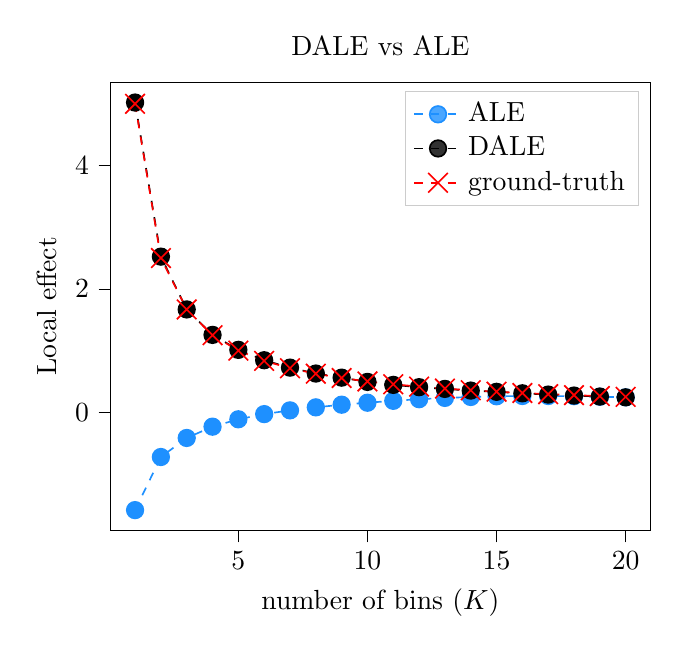
\begin{tikzpicture}

\definecolor{darkgray176}{RGB}{176,176,176}
\definecolor{dodgerblue}{RGB}{30,144,255}
\definecolor{lightgray204}{RGB}{204,204,204}

\begin{axis}[
legend cell align={left},
legend style={fill opacity=0.8, draw opacity=1, text opacity=1, draw=lightgray204},
tick align=outside,
tick pos=left,
title={DALE vs ALE},
x grid style={darkgray176},
xlabel={number of bins \(\displaystyle (K)\)},
xmin=0.0499999999999999, xmax=20.95,
xtick style={color=black},
y grid style={darkgray176},
ylabel={Local effect},
ymin=-1.9158582242841, ymax=5.35027643439794,
ytick style={color=black}
]
\addplot [semithick, dodgerblue, dashed, mark=*, mark size=3, mark options={solid}]
table {%
1 -1.58557937616219
2 -0.724469128659219
3 -0.415970121031068
4 -0.232936150463663
5 -0.11325432870959
6 -0.02954530629491
7 0.0314157941118509
8 0.0799920748845464
9 0.122926085482714
10 0.155053447821085
11 0.186088568383995
12 0.211864987771331
13 0.233108878251814
14 0.247869171569635
15 0.259566596177554
16 0.264108921400541
17 0.263569771086526
18 0.260892620884744
19 0.252751953555994
20 0.242460730712491
};
\addlegendentry{ALE}
\addplot [semithick, black, dashed, mark=*, mark size=3, mark options={solid}]
table {%
1 5.01999758627603
2 2.52286238913594
3 1.66707743267251
4 1.25440995432319
5 1.01184271234757
6 0.843722016967248
7 0.72371907999776
8 0.627936897660279
9 0.561288325580339
10 0.492398374084428
11 0.444051023514039
12 0.4070407257714
13 0.379038857924861
14 0.351678147881759
15 0.331857705495926
16 0.307844113455479
17 0.286910008925387
18 0.270908782811331
19 0.254748495290572
20 0.24246073071272
};
\addlegendentry{DALE}
\addplot [semithick, red, dashed, mark=x, mark size=5, mark options={solid}]
table {%
1 5
2 2.5
3 1.66666666666667
4 1.25
5 1
6 0.833333333333333
7 0.714285714285714
8 0.625
9 0.555555555555556
10 0.5
11 0.454545454545455
12 0.416666666666667
13 0.384615384615385
14 0.357142857142857
15 0.333333333333333
16 0.3125
17 0.294117647058824
18 0.277777777777778
19 0.263157894736842
20 0.25
};
\addlegendentry{ground-truth}
\end{axis}

\end{tikzpicture}
}
  \caption[Example comparison]{(Left) The black-box function \(f\) of
    Section~\ref{sec:4-3-robustness}. (Right) Estimation of the local
    effect of the first bin for DALE and ALE, for varying number of
    bins \(K\).}
  \label{fig:example-different-bins}
\end{figure}
